\pagestyle{IHA-fancy-style}
\lhead{\textsf{Chapter VI}}
\rhead{\textsf{Synthetic \& Natural PVC Operon Regulation}}


\chapter{Synthetic \& natural PVC operon regulation}\label{regulation}

\epigraph{\emph{``...cells are very tiny, but they are very active; they manufacture various substances; they walk around; they wiggle; and they do all kinds of marvellous things...''}}{\textit{Richard P. Feynman}}

\section{Introduction}
PVCs were originally identified due to their toxic effects in a ``Rapid Virulence Annotation" screen \citep{Waterfield2008, Yang2006}. The ``RVA" screen examined a cosmid library comprised of \emph{Photorhabdus} sequences which were heterologously expressed in ordinary lab \emph{E. coli},  and tested against insects, nematodes, amoebae and macrophages for activity. Should the cosmid clone contain a genomic region which encoded a toxin or virulence factor, assorted lethalities or morbidities could be detected in the screened cell or organism types.

PVC bearing cosmids were obtained in various states of completeness, often with the 5' regions deleted, though enough functional cosmids were recovered to produce the first work on the PVCs \citep{Yang2006}. The frequency of deletion of regions of the PVC bearing cosmids suggested that intact cosmids were not easily recovered in \emph{E. coli} and had a toxic effect. This was borne out by steadily decreasing viability of certain cosmid clones when routinely cultured for experiments.

The precise basis of this toxicity is still unknown. One hypothesis was that the PVCs (being somewhat phage-like), were potentially lysing the cells that produced them (some of the operons are also found in close register to holin-lysin pairs). Since the PVCs were obtained in the cosmids with their own promoters and regulatory signals, their expression was likely uncontrolled or `haywire', n a non-\emph{Photorhabdus} host, even though \emph{Photorhabdus} and \emph{E. coli} are both Enterobacterial.

However, there were a number of PVC operons, that despite being cloned in their entirety, did not cause such pronounced toxicity. Inferring from RNAseq data for the PVCs in \emph{Photorhabdus}, many PVC operons are silent under normal culture conditions, or expressed at lower levels. These silent operons, while propagable, were of limited use for further study since they are not producing active PVCs. Thus, one of the earliest aims in this project was to explore methods for more reliable and controllable heterologous expression of PVCs on demand. This is also desirable as the cosmid clones often contain flanking sequence to the PVCs, which could contain genes/proteins which confound assays.

In addition to genetically engineering control of PVC sequences, a better understanding of the natural expression patterns and regulation of the PVCs is also desirable. Why, for example, are some PVCs expressed to the point of toxicity in standard culture conditions, whilst others are entirely silent?

The wide variety of PVC loci suggests they are responding to a plethora of environmental cues to trigger their deployment, and thus their expression patterns could be very prescriptive. Furthermore, due in large part to its esoteric lifestyle, \emph{Photorhabdus} is known to exhibit a significant degree of population heterogeneity in many other phenotypes \citep{Langer2017, Heinrich2016}. This suggests that not only might the PVCs expression/deployment depend on environmental cues, but that it may also depend on culture conditions (such as density), growth phase, and phenotypic state (\emph{Photorhabdus} exists as `primary' and `secondary' cells \citep{Boemare1988}). Its primary/secondary variability has been shown to manifest in various phenotypes. For instance, the bulk of the bioluminescence produced by \emph{Photorhabdus} cultures is attributable to the primary (1$^{\circ}$) cells \citep{Boemare1988, AKHURST1980}, the majority of anthraquinone-based pigmentation occurs in 1$^{\circ}$ cells  with a particular metabolic suppression in 2$^{\circ}$ whereby the same transcription factor \emph{AntJ} has diametrically opposite effects in primaries versus secondaries \citep{Heinrich2016, Langer2017}. Among other examples include the differential deployment of a variety of proteolytic enzymes \citep{Marokhazi2004}, a global shift in fundamental biochemical processes such as respiration \citep{Smigielski1994} and production of secondary metabolites \citep{Turlin2006}, and, perhaps most prominently and significantly of all, 2$^{\circ}$ cells are incapable of association with the nematode vector. Thus, a second aim of this chapter is to asses the PVC operons for any heterogeneity in expression among a bacterial population.

Little is precisely known about the choreography of PVC (and, more broadly, many caudate structure's) expression and assembly. The T4 phage is the best understood, as evidenced in \vref{t4assemblyflowchart}, however, T4 genetics are quite far removed from that of simple caudate structures, with a much larger genome and both ``early" and ``late" expression profiles \citep{OFarrell1973}. The best indication for the regulatory system in the PVCs comes, once again, from the work of \cite{Hurst2007a, Hurst2004}. In the original studies that attempted to elucidate the structure, expression of the Afp cluster was only achievable when an additional protein from the pADAP plasmid was also heterologously expressed. Namely \emph{anfA1}, the protein was identified upstream of the Afp cluster as part of a pair of genes (the other is termed \emph{anfA2}), which contained a NusG-like domain with some sequence similarity to the RfaH transcript elongation factor, and over-expression resulted in a concomitant over-expression of the Afp itself. To slightly confound these findings however, \cite{Hurst2018} have identified another Afp locus in \emph{Serratia proteamaculans} strain AGR96X, termed AfpX, which has a disparate 5' region, and responds to mitomycin C induction (unlike the Afp), suggesting it has somewhat different regulatory mechanisms. It does, however, retain the 2 \emph{anfA} loci upstream, and associated \emph{ops} binding site (discussed in the next paragraph).

RfaH, a specialised version of NusG (a generalist transcription factor) has been shown to be important in the expression of long operons \citep{Bailey1996}, by prolonging the transcripts and preventing the polymerase from prematurely dropping off the strand (increasing processivity), ordinarily brought about by Rho-dependent termination. RfaH is recruited to the RNA polymerase transcript elongation complex (TES) at a specific DNA motif called the he \emph{ops} (operon polarity suppression) site (which in \emph{E. coli} has the sequence \texttt{5'-GGCGGTAGnnTG-3'}). Operon polarity refers to the mechanism by which under `ordinary' expression circumstances, Rho proteins bind to exposed mRNA regions brought about by ribosome halting, but RNA polymerase processing continuing. In prokaryotes, translation occurs directly on the nascent 5'-end of the transcript as it is produced from the RNA polymerase, meaning the 2 complexes are in close register the majority of the time. However, when a stop codon in the nascent RNA is met by the ribosom - it halts - meanwhile, the RNA polymerase continues to process, and therefore a small gap of exposed RNA can form. The Rho proteins bind to this region of exposed RNA, track along it, and disrupt the RNA polymerase, preventing/reducing the `unintended' transcription of downstream genes. This reduction in expression of downstream regions is what is known as operon polarity \citep{Santangelo2008, Adhya1974, Banerjee2006, Nudler2002}. The \emph{ops} site therefore earns its name by mediating a counteracting (``suppressing") effect to this `premature' transcription termination for long operons, by ensuring that the RNA polymerase stays attached to the template and continues to process the mRNA for a full length operon. Transcription is enhanced for roughly 20 kb downstream \citep{Artsimovitch2002, Leeds1996, Leeds1997}, which is the approximate minimal length of the structural components of a PVC operon. Effectors for PVCs often appear with their own promoters and can be transcribed independently of the rest of the operon, as seen in previous transcriptomic studies of \emph{Photorhabdus}.


\begin{figure}[h]
    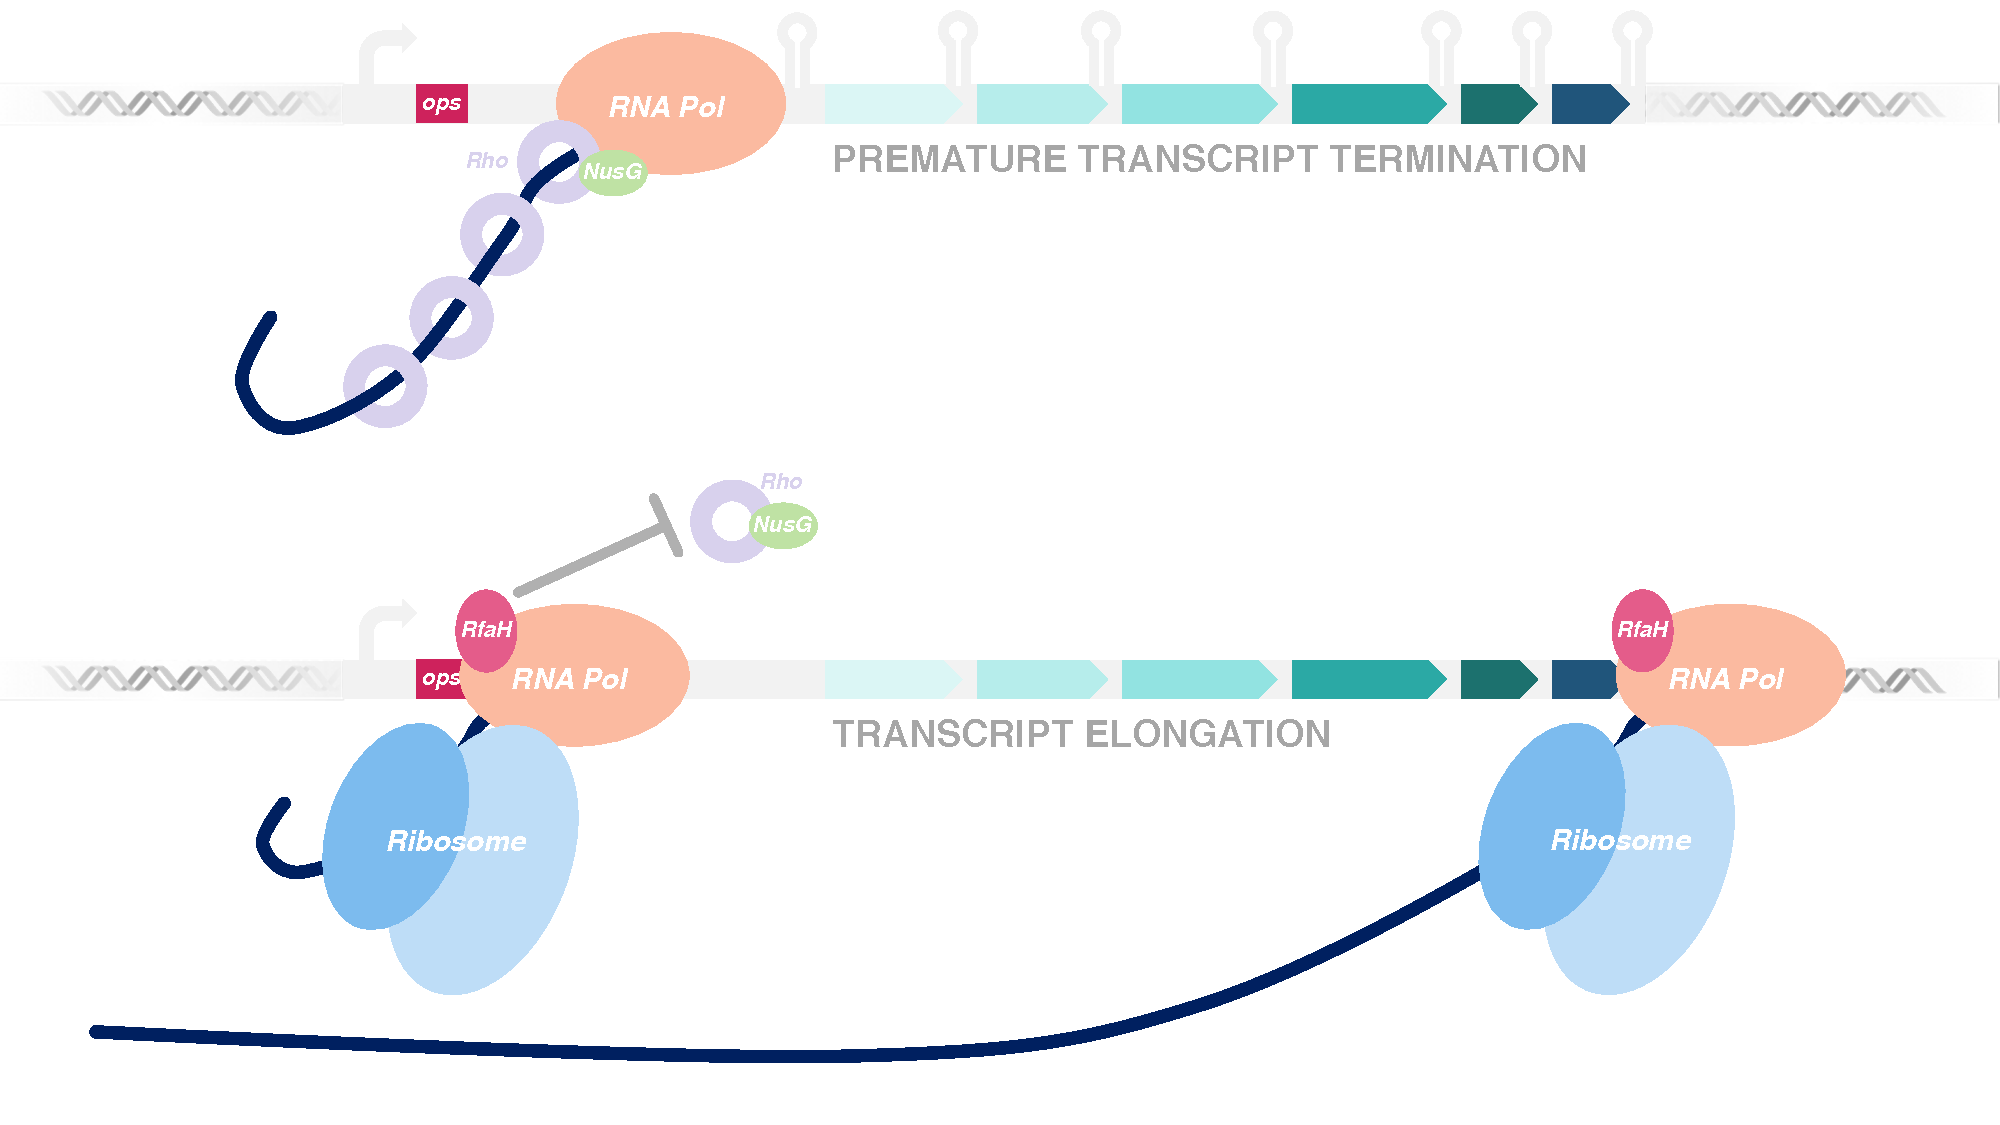
\includegraphics[width=\textwidth, clip, trim={0 -10 0 0 }]{/Users/joehealey/Documents/Warwick/PhD/Thesis/chapters/chapter6/img/RfaH_mechanism.pdf}
    \captionsetup{singlelinecheck=off, justification=justified, font=footnotesize, aboveskip=0pt}
    \caption[Schematic diagram of the mechanism of RfaH-mediated transcript elongation]{\textsc{\normalsize A schematic diagram depicting elongation mechanism of RfaH.} \vspace{0.1cm} \newline A schematic diagram to demonstrate the transcript elongation effect of RfaH. In the upper panel, in the absence of RfaH, the transcript terminates early (thus a high degree of polarity) when encountering terminators in the RNA structure. NusG and Rho proteins complex with the polymerase and the nascent strand, blocking any translation. In the lower panel, with RfaH present and recruited to the polymerase at the \emph{ops} site, and the protein blocks the activity of Rho and NusG proteins, and in complex with the RNA polymerase and ribosome, increases the processivity of the polymerase, traversing through terminators. RfaH is believed to have some activity in direct loading of the ribosome on to the RNA strand. Diagram based on Figure 1 from \cite{Hu2017}. }
\label{rfahmechanism}
\end{figure}


Gene clusters which have been demonstrated to be dependent on RfaH, include the LPS core, exopolysaccharides \citep{Wilkinson1972}, haemolysin toxins \citep{Landraud2003, Leeds1996, Leeds1997} and the F-type conjugation pilus. The \emph{ops} site which RfaH obligately depends upon has also been found in \emph{Shigella flexneri}, \emph{Yersinia enterocolitica}, \emph{Vibrio cholerae} and \emph{Klebsiella pneumoniae} polysaccharide synthesis clusters, as well as the RP4 fertility operon of \emph{Pseudomonas aeruginosa} \citep{Bailey1997} - and of course the \emph{S. entomophila} Afp \citep{Hurst2007a}. The \emph{ops} site is therefore widespread in the \emph{Proteobacteria}, and possibly further. Deletion of either the \emph{ops} site, or RfaH itself results in equivalent reduction in transcription \citep{Bailey1997}. Interestingly, the \emph{ops} site has also been identified as part of a larger 39 bp sequence known as the ``JUMPStart" sequence, which consists of a conserved but somewhat degenerate GC-rich hairpin structure immediately prior to the \emph{ops} sequence. The JUMPStart sequence has been detected in most of the examples listed previously \citep{Wang1998}. It is not, however, found in the \emph{tra} operon that gives rise to the F pilus, nor in the typical \emph{hyl} haemolysin operon \citep{Nieto1996} - however, \cite{Leeds1997} showed the \emph{hyl} operon of the \emph{E. coli} J96 strain \emph{does} use a full JUMPStart motif). Why the JUMPStart sequence, which can be thought of as an extended \emph{ops} sequence, is necessary, is not clear, since the \emph{ops} site is evidently sufficient for RfaH recruitment and long operon expression in some cases.

Interestingly, literature such as the papers by \cite{Bailey1996} and \cite{Santangelo2002} note that RfaH regulation seems to also be a hallmark of long operons whose products are destined for the extracellular environment/membrane (e.g. LPS, pili, secreted enzymes), though if there is a strict dependence/relationship on this is not clear, and there is certainly no understood mechanism; it is tempting to speculate that this might be the case for the PVCs and Afps which are also destined for the extracellular environment, however. 

Finally, therefore, another aim for this chapter was to investigate any potential roles RfaH might have in PVC mechanistics. 

\subsection*{Chapter Aims:}
\begin{itemize}
	\item Engineer controllable PVC expression constructs.
	\item Examine the natural regulation and expression patterns of PVCs in \emph{Photorhabdus} populations.
	\item Investigate the putative role of RfaH-like proteins in PVC regulation.
\end{itemize}
\clearpage


\section{Experimental procedures}

\vref{workflows} depicts a high level overview of the experimental threads running through this chapter as it contains areas of different focus. The chapter is broadly divided in to efforts to reconstitute the PVCs heterologously in \emph{E. coli} through a number of methods (2 blue threads), and similarly, efforts to understand the activity of the natural expression system in several ways (2 orange threads).

\vspace{0.2cm}
\begin{figure}[h!]
\centering
    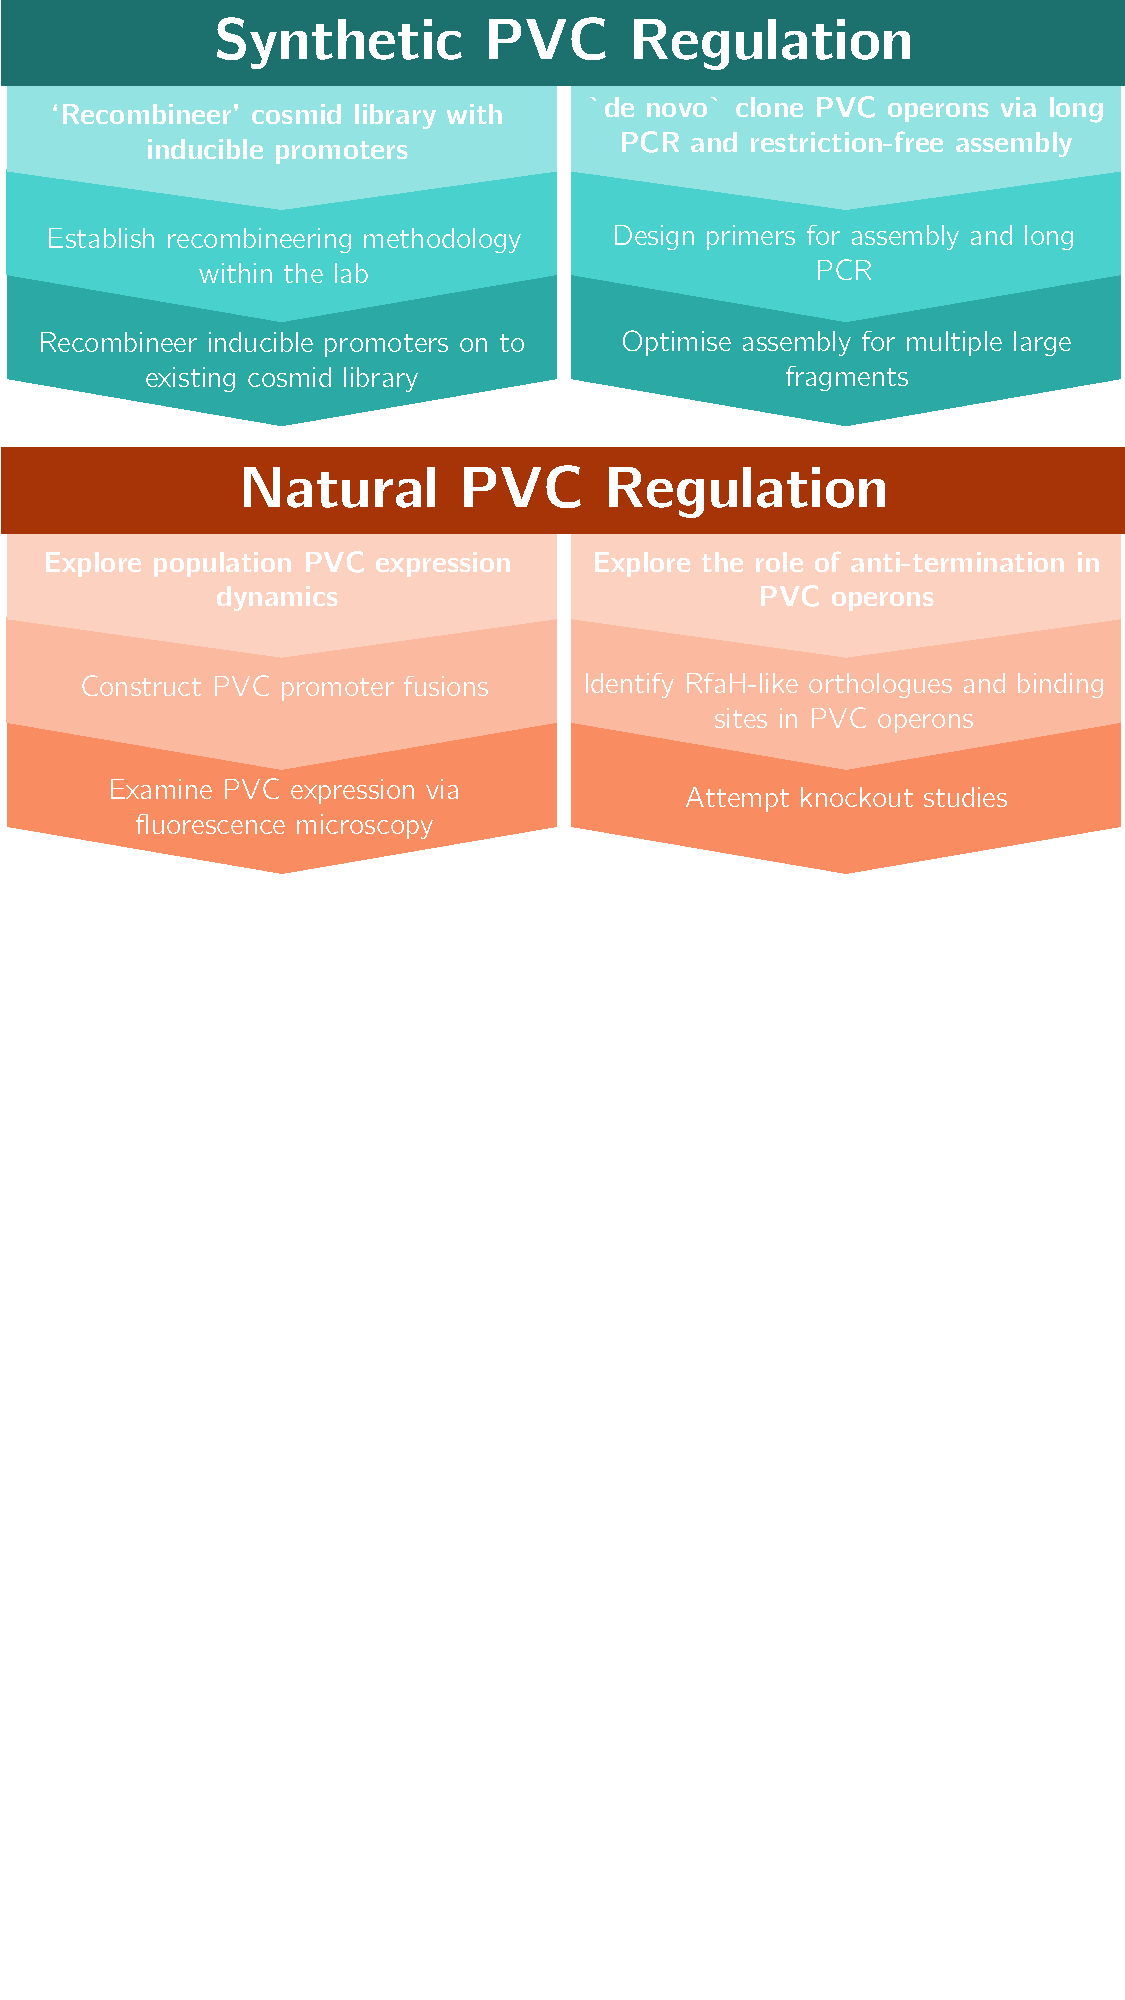
\includegraphics[width=0.9\textwidth, clip, trim={0 520 0 0 }]{/Users/joehealey/Documents/Warwick/PhD/Thesis/chapters/chapter6/img/Workflows.pdf}
\captionsetup{singlelinecheck=off, justification=justified, font=footnotesize, aboveskip=15pt}
\caption[Flowchart of work threads for PVC regulation studies]{\textsc{\normalsize A high level flowchart of the threads for studying PVC regulation.} \vspace{0.1cm} \newline A high level flowchart showing the experimental threads for this chapter. The upper blue chart shows the efforts towards making controllable synthetic PVC constructs through recombineering and synthetic fragment assembly approaches. The lower orange chart depicts the 2 primary packages of work undertaken to probe the natural regulatory system of the PVCs, and the `sub-threads' within this. Namely, construction of promoter fusions allowing for studies of the population heterogeneity (or lack thereof) in PVC expression, and an examination of AnfA1 orthologue control of PVCs within \emph{Photorhabdus}. }
\label{workflows}
\end{figure}




\subsection{Cloning and engineering PVC operons}\label{cloningPVCs}
As discussed in the introduction to this chapter, the only existing heterologous expression system that was available was the `raw' cosmid clones from the initial identification of the PVCs. The most bioactive of these, PVCpnf from the \emph{P. asymbiotica} ATCC43949 strain, was also the most genetically unstable, and over time freezer stocks had dwindled since it could not be easily propagated. This section will explore the experimental efforts undertaken to try and reconstruct these long operons in \emph{E. coli}.

All of the techniques that follow have specifically avoided attempts at classically cloning PVCs, instead opting for techniques that rely on homologous recombination. Classical restriction based cloning was ruled out early on, as the operons are very long and rich in restriction sites that rendered a lot of the reliable `standard' lab enzymes no longer an option, especially as the operons would probably need to be cloned in several chunks. Ideally, a robust technique was desired that would allow any of the PVC operons to be cloned. A dependence on particular restriction sites might preclude certain operons from being cloned. Additionally, it was unknown whether there was internal structure to the operons such as internal promoters. Certain proteins are certainly transcriptionally coupled for example, so the incorporation of restriction sites and any intervening spaces could impact the expression and assembly of the PVCs. However, a previous post-doc of the group did achieve the cloning of a single operon in this manner separately, contemporary with the efforts here. While this demonstrates in principle that classical cloning is a viable approach for constructing these operons, a previous attempt by the same lab at an alternative operon had lead to various assembly errors internal to the sequence, and rendered the construct unusable.

Moreover, much of the existing literature for cloning of long operons pointed to homologous recombination based techniques as a promising approach for subcloning recalcitrant or difficult targets (for example, \cite{Wang2016, Garcia2004}, both of whom present novel DNA capture techniques). Despite the interest in bioprospecting or `genome mining' (combing genomes for biosynthetic gene clusters of interest) of late \citep{Ziemert2016, VanLanen2006, Netta2009, Lautru2005, Bergmann2007, Wenzel2009, Charlop-Powers2014}, due in no small part to the explosion of interest and improved capabilities in (meta)genomics, it is still non-trivial to manipulate sequences of this size.

\subsubsection{Recombineering}\label{recombineering}
Since the original cosmids containing segments of the captured genome were available, it was decided that a promising approach might be to try and engineer control in to the replicons that were already obtained, attributing the reductions in cell viability to simple uncontrolled expression via natural promoters.

Recombineering is a long standing technique for `recombination-mediated genetic engineering' (hence the name). It relies on the use of 3 phage $\lambda$ proteins, named Gam, Beta, and exo, to facilitate the incorporation of segments of linear DNA with 5' and 3' homologous stretches to an insert site of choice. Perhaps its most `famous' use is the technique of choice for the generation of the Keio collection of \emph{E. coli} knockouts, which first defined a minimal essential genome \citep{Baba2006}. Two major alternative techniques exist, using 2 different enzyme sets: RecET from the Rac prophage and ``Lambda-Red", which is the mechanism discussed here. Exo is an exonuclease responsible for creating 3' overhangs (it has 5' $\rightarrow$ 3' exonuclease activity, hence its name); Beta is a single strand binding protein which stabilises these overhangs so that they aren't degraded by host enzymes and recombination can occur more efficiently. To further improve the recombination efficiency, the Gam protein inhibits the RecBCD nuclease complex \citep{Yu2000}. \vref{recombineeringmechanism} shows a schematic of how the process works.


\begin{figure}[p]
    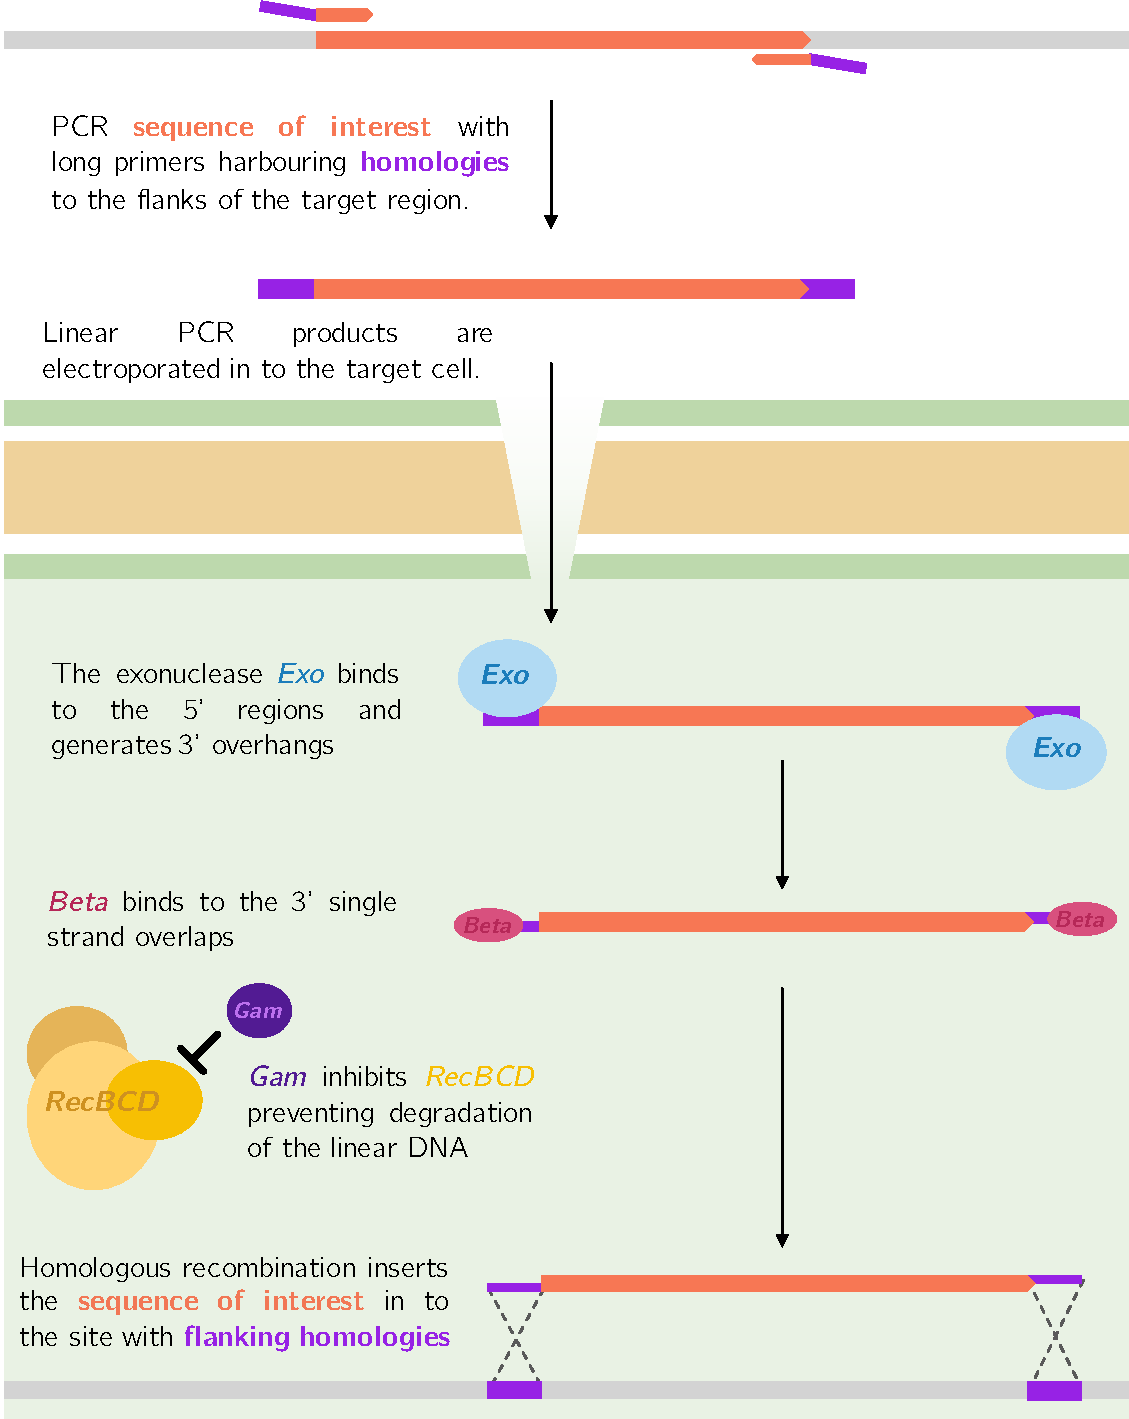
\includegraphics[width=\textwidth, clip, trim={0 0 0 0 }]{/Users/joehealey/Documents/Warwick/PhD/Thesis/chapters/chapter6/img/Recombineering.pdf}
    \captionsetup{singlelinecheck=off, justification=justified, font=footnotesize, aboveskip=10pt}
    \caption[Recombineering mechanism of action]{\textsc{\normalsize The mechanism of action for ``$\lambda$ Red"-based recombineering.} \vspace{0.1cm} \newline ``$\lambda$ Red"-mediated engineering is performed by amplifying an insert sequence of interest using primers with overhanging sequences (up to $\approx$ 50 bp), which are homologous to the flanking regions of the intended insert site. The linear DNA is electoporated in to the desired cells. Phage $\lambda$ proteins are induced in the cells prior to making them electrocompetent, and thus the exonuclease Exo is readily available to begin digesting the linear DNA. As it does so, single stranded binding proteins, Beta, bind the overhangs to stabilise the fragment and prevent degradation. The Gam protein which is also expressed with Beta and Exo, inhibits the Rec nuclease complex to preserve the linear DNA and improve efficiency. Finally, the sequence of interest recombines with the target site as determined by the flanking regions.}
\label{recombineeringmechanism}
\end{figure}


\myparagraph{Chromosomal engineering}
Since recombineering was a new technique in the lab, a working protocol was first devised by attempting to knock out chromosomal targets. Three chromosomal \emph{E. coli} targets were chosen as trials. Initially the \emph{att} site used for phage insertion was chosen as it was proposed that this should be non-essential. All attempts to engineer this site failed however, and thus it was hypothesised that perhaps this region was too `genetically active', possibly with prophages moving, to be engineerable. Instead, the 3 sites chosen to replace it were the \emph{hyfC} locus, which encodes part of the hydrogenase complex, since in the Keio collection data this was scored as the least essential gene (and thus should be easy to knock out) \citep{Yu2000}. Moreover, the hydrogenase is only transcriptionally active under anaerobic conditions \citep{Skibinski2002}, which suggested that the region would be experiencing less `cellular traffic', such as RNA polymerases, thus making recombination as simple as possible. Next, using the same approach \emph{speB} was identified as the next-least essential protein. \emph{speB} encodes an `agmatinase' enzyme, which is responsible for producing putrescine and urea from the precursor agmatine \citep{Szumanski1990}. Lastly, the endonuclease encoded by the gene \emph{endA} was targeted for knockout. The primers in \vref{specprimers}, show the sequences used to amplify antibiotic resistance cassettes encoded on the helper plasmids pJET-FRT-Kan and pJET-FRT-Cat. These plasmids carry an antibiotic cassette flanked by conserved primers that can be used to amplify either, and Flp-flippase recombination sites which can be used to optionally `pop out' the introduced marker to create (semi)clean deletions. Note, \emph{endA} is denoted as a `pseudo' \emph{endA} in the table with a $\psi$, since the protein is actually mutated in laboratory \emph{E. coli} already. to reduce its proteolytic activity, however the locus is still mostly present.

Recombineering was performed as outlined in \vref{recombineering}. Successful colonies were screen with the primers used to amplify the cassette, and a number of successful colonies were observed for all 3 inserts. To be certain that the insert was correct, flanking primers to the \emph{hyfC} locus were designed $\approx$ 200 bp up and downstream of the insertion site, and used to confirm the correct insertion via Sanger sequencing.

With the technique successfully applied in the test case, the protocol was adapted and applied to recombineering the cosmids.


\begin{figure}[h]
  \centering
    \frame{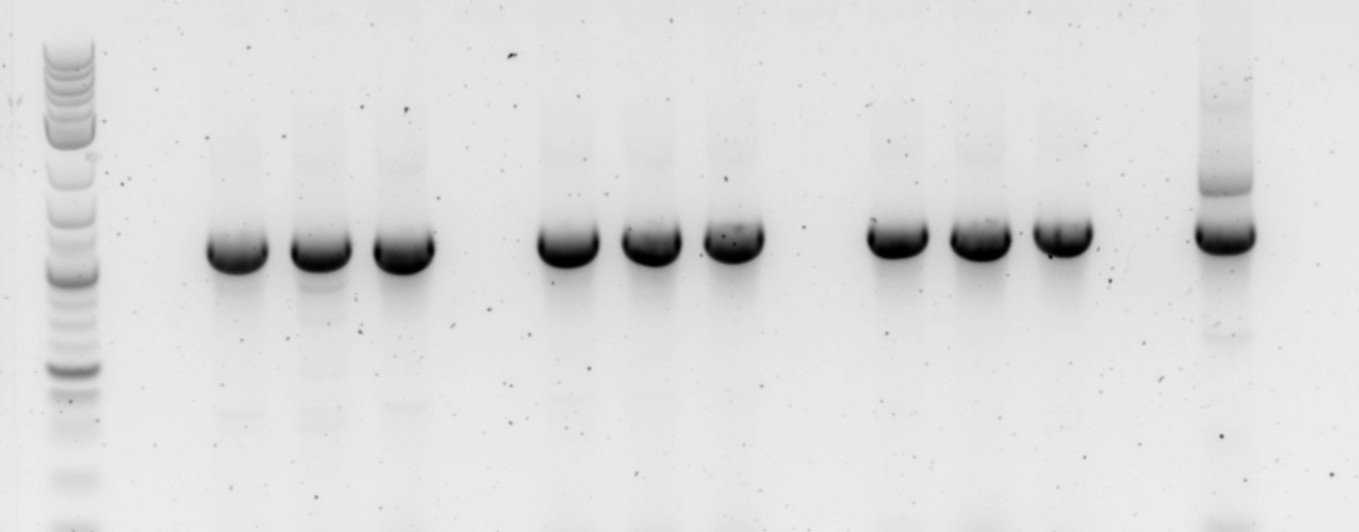
\includegraphics[width=0.8\textwidth, clip, trim={10 110 1 150 }]{/Users/joehealey/Documents/Warwick/PhD/Thesis/chapters/chapter6/img/Recombineeringproof.png}}
    \put(-335,51){\rotatebox{45}{\textbf{Marker}}}
    \put(-370,50){\textbf{kbp}}
    \put(-364,32){\textbf{1.2}\customarrow{1pt}{180} }
    \put(-364,20){\textbf{1.0}\customarrow{2pt}{200} }
    \put(-364,0){\textbf{0.5}\customarrow{1pt}{180} }
    %
    \put(-40,51){\rotatebox{45}{\textbf{+ Control}}}
    \put(-15,51){\rotatebox{45}{\textbf{- Control}}}
    %
    \put(-277, 65){\textbf{\textit{hyfC}}}
    \put(-293, 62){\obscure[black]{2cm}{0.03cm}}
    \put(-287, 51){\textbf{1}}
    \put(-266, 51){\textbf{2}}
    \put(-245, 51){\textbf{3}}
     %
    \put(-191, 65){\textbf{\textit{speB}}}
    \put(-208, 62){\obscure[black]{2cm}{0.03cm}}
    \put(-202, 51){\textbf{1}}
    \put(-181, 51){\textbf{2}}
    \put(-160, 51){\textbf{3}}
    %
    \put(-109, 65){\textbf{\textit{endA}}}
    \put(-125, 62){\obscure[black]{2cm}{0.03cm}}
    \put(-119, 51){\textbf{1}}
    \put(-98, 51){\textbf{2}}
    \put(-77, 51){\textbf{3}}
    
    \captionsetup{singlelinecheck=off, justification=justified, font=footnotesize, aboveskip=10pt}
    \caption[Successful engineering of \emph{E. coli} chromosomal genes]{\textsc{\normalsize Validation of recombineering techniques for chromosomal targets.} \vspace{0.1cm} \newline This gel shows the first indication that the recombineering protocol had finally been sufficiently optimised and was working satisfactorily to test against PVC elements in subsequent study. The gel shows the result of colony PCR against DH10$\beta$, demonstrating insertion of a kanamycin cassette in place of the genes \emph{hyfC}, \emph{speB} and \emph{endA}. The helper plasmid which bears the kanamycin cassette is used as a positive control. Expected band size was 1168 bp.}
\label{recombineeringmechanism}
\end{figure}

\myparagraph{Cosmid engineering}
\addfloat{Diagram of the devised method for engineering cosmids}

pkD56?
Dy380?
% If not including, make sure to remove from section 2.2.8.2 Electroporation-Recombination using λ-Red Bearing Plasmids and 
% 2.2.8.3 Electroporation-Recombination with λ-Red Chromosomal Strains

\subsubsection{Gibson assembly}
To attempt to clone the PVCs in a manner that would not depend on restriction sites, a process of construct creation using the fairly new ``Gibson" assembly technique was tested and optimised. Gibson assembly has been popularised ever since the advent of the first synthetic genome produced by \cite{Gibson2010c, Gibson2009a} (hence the name). The method promises \emph{in vitro} assembly in a largely sequence-agnostic manner, crucially without the requirement for restriction sites, for fragments up to the hundreds of kilobase range. The technique works by mixing overlapping linear DNA, which have complementary ends (in a manner similar to recombineering), and using 3 isothermal enzymes to create `sticky ends' which anneal, are `gap-filled' and ligated, all in a single reaction pot. Firstly, T5 exonuclease creates the 3' overhangs, exposing the complementary overlaps as stretches of single stranded DNA. These complementary regions base pair, and the T5 nuclease is displaced by the Phusion polymerase (or \emph{Taq}), which `back fills' the gaps created by the exonuclease beyond the overlap sites. This leaves a double stranded fusion product of the adjoining fragments, but with disconnected backbones. As the last step of the isothermal assembly reaction, the \emph{Taq} ligase enzyme seals the backbones, yielding 2 fully connected fragments with a high degree of sequence fidelity at the joins.

Several attempts were made, initially following the manufacturers guidelines, but later, additional optimisations were included which improved assembly size and efficiency. The most optimal of these is the protocol given in \vref{gibson}. Briefly, substantially longer primers than the suggested overlaps were used - this was for 2 reasons. Firstly, the longer (70 bp) primers (35 bp of each neighbouring fragment), were considerably easier to PCR with the NEB Q5 enzyme, especially at longer lengths, where the shortest PCR fragment was $\approx$ 4.5 kb. Secondly, the increased overlaps provided the first indications of any assembly whatsoever, suggesting better efficiency, especially for such long fragments. The suggested overlaps of $\approx$ 12-18 bp were attempted initially, using standard \emph{in silico} construction tools, but yielded no assembled colonies at all.

\begin{figure}[p]
\centering
  \begin{subfigure}{\textwidth}
    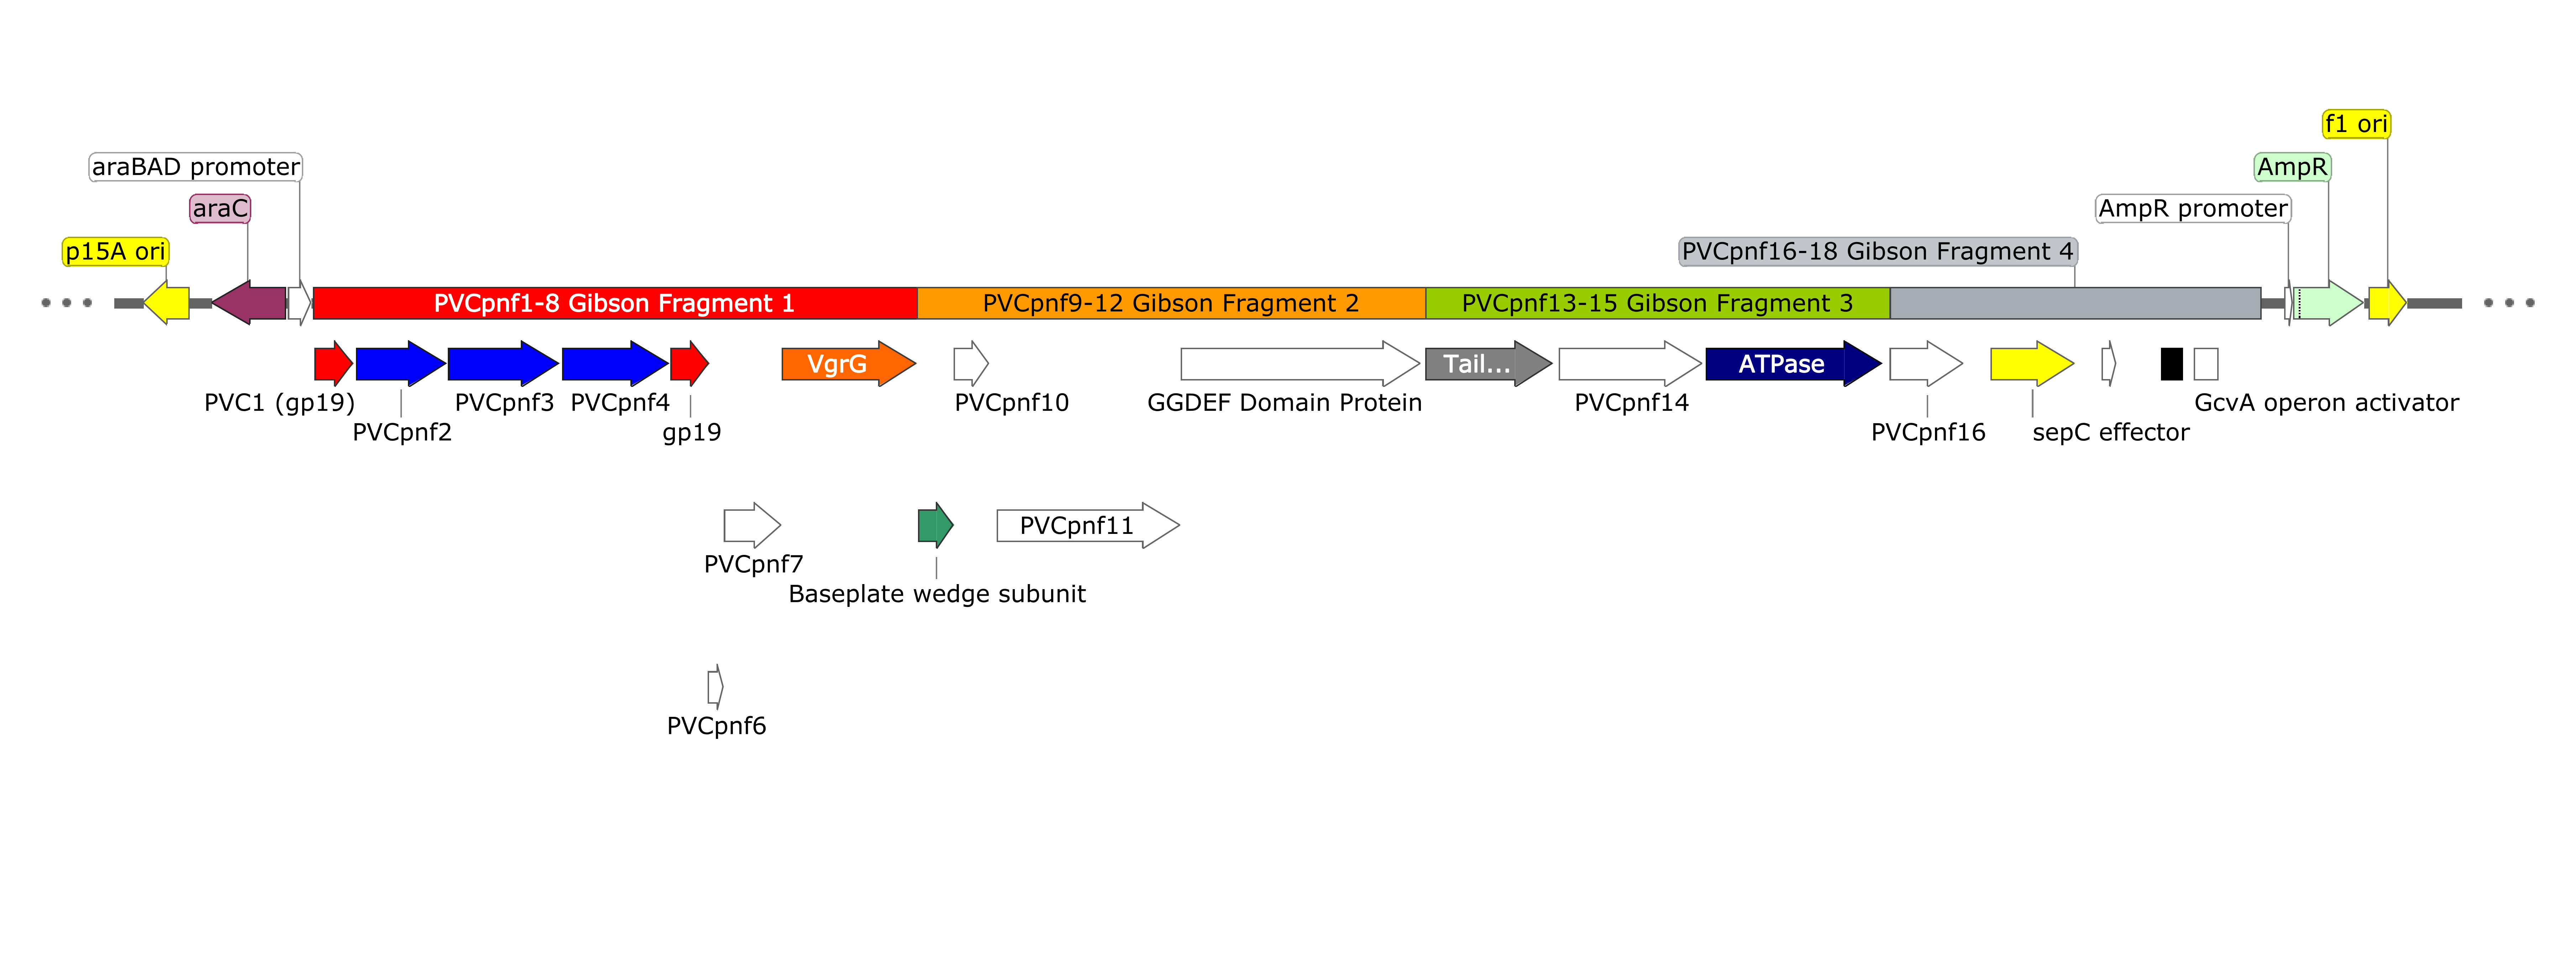
\includegraphics[width=\textwidth, clip, trim={20 140 20 65}]{/Users/joehealey/Documents/Warwick/PhD/Thesis/chapters/chapter6/img/GibsonIdealMap.png}
    \captionsetup{singlelinecheck=off, justification=centering, font=footnotesize, aboveskip=10pt}
    \caption{}
    \label{gibsonidealmap}
  \end{subfigure}

  \begin{subfigure}{\textwidth}
    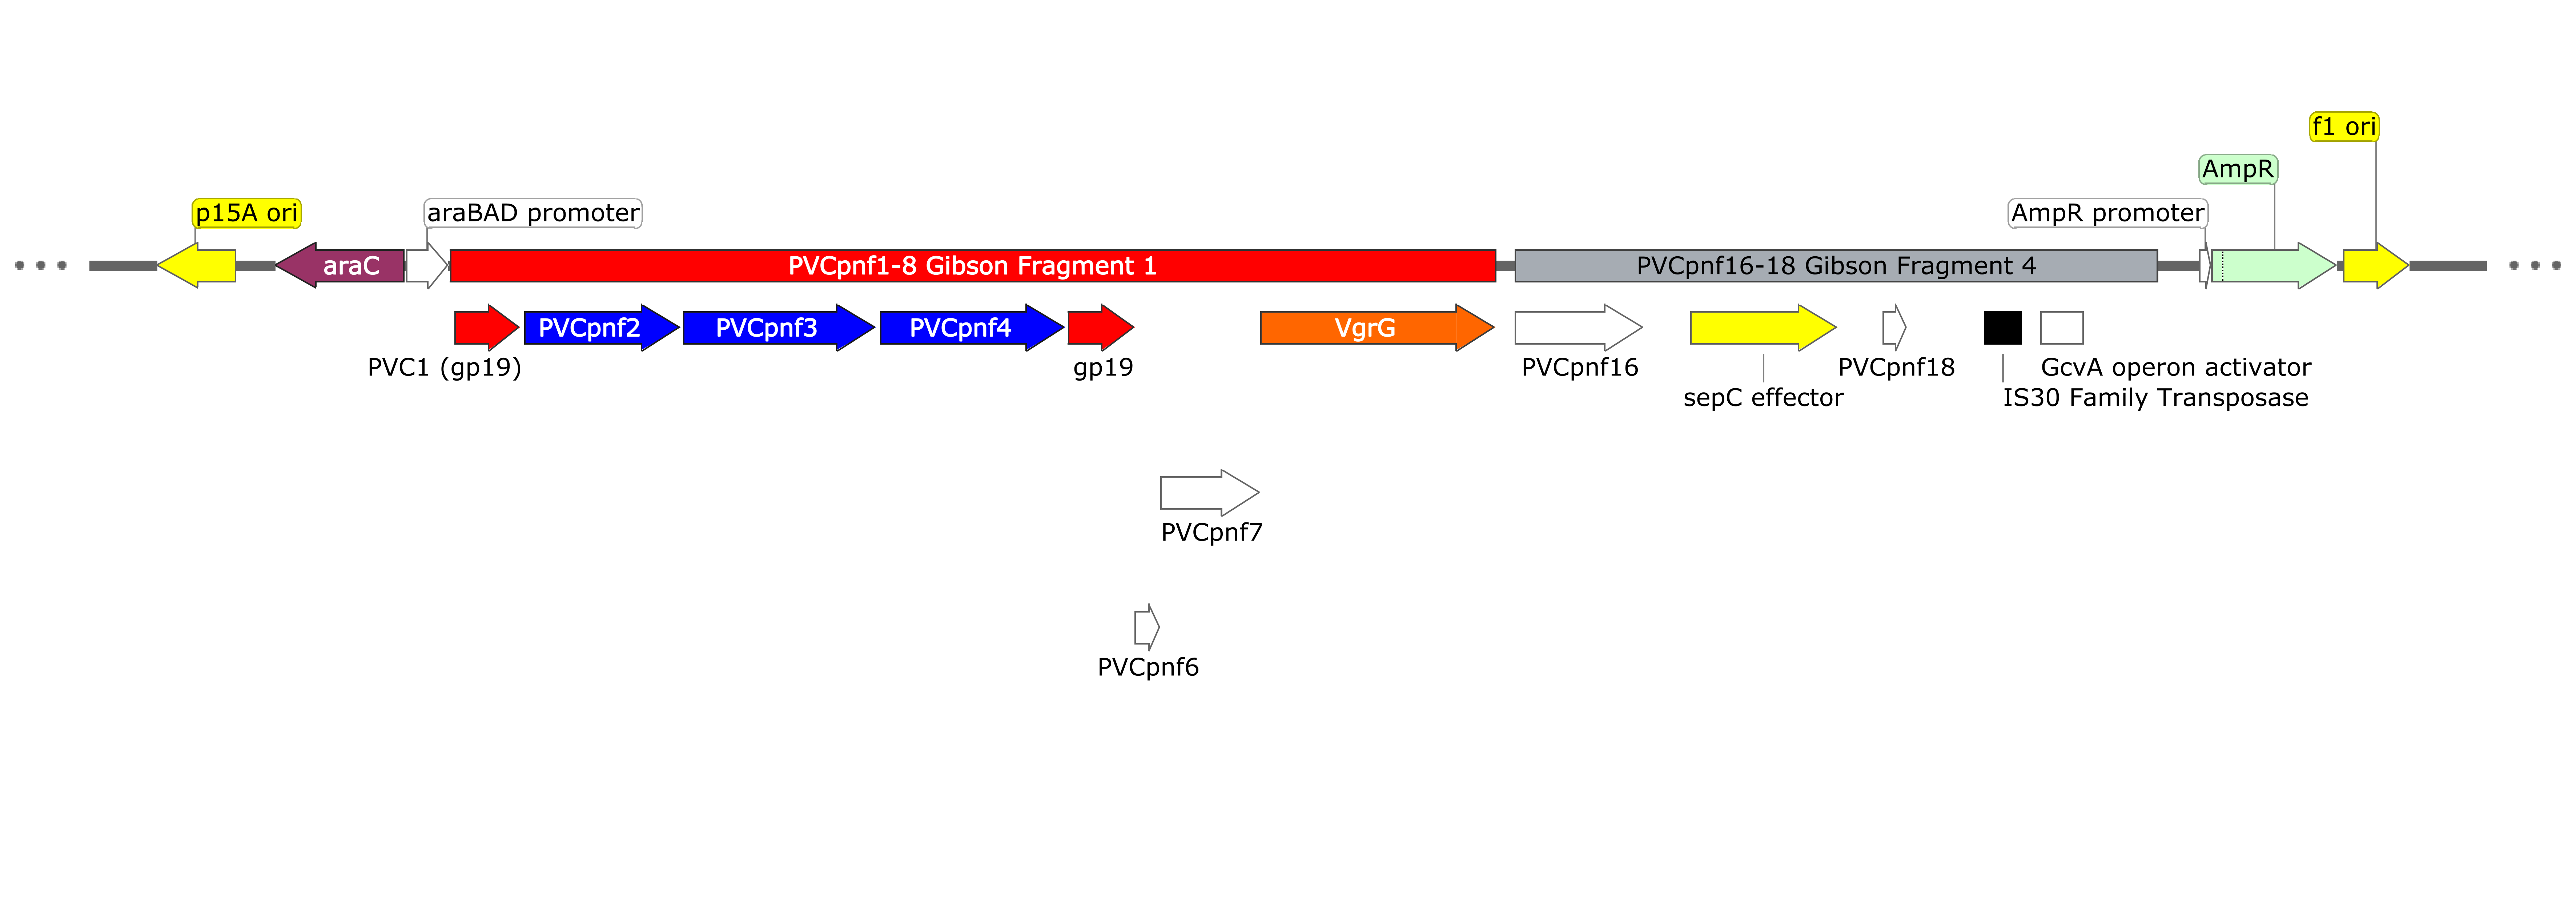
\includegraphics[width=\textwidth, clip, trim={0 140 0 65}]{/Users/joehealey/Documents/Warwick/PhD/Thesis/chapters/chapter6/img/GibsonB_bestcontigMap.png}
    \captionsetup{singlelinecheck=off, justification=centering, font=footnotesize, aboveskip=10pt}
    \caption{}
  \end{subfigure}

  \begin{subfigure}{\textwidth}
    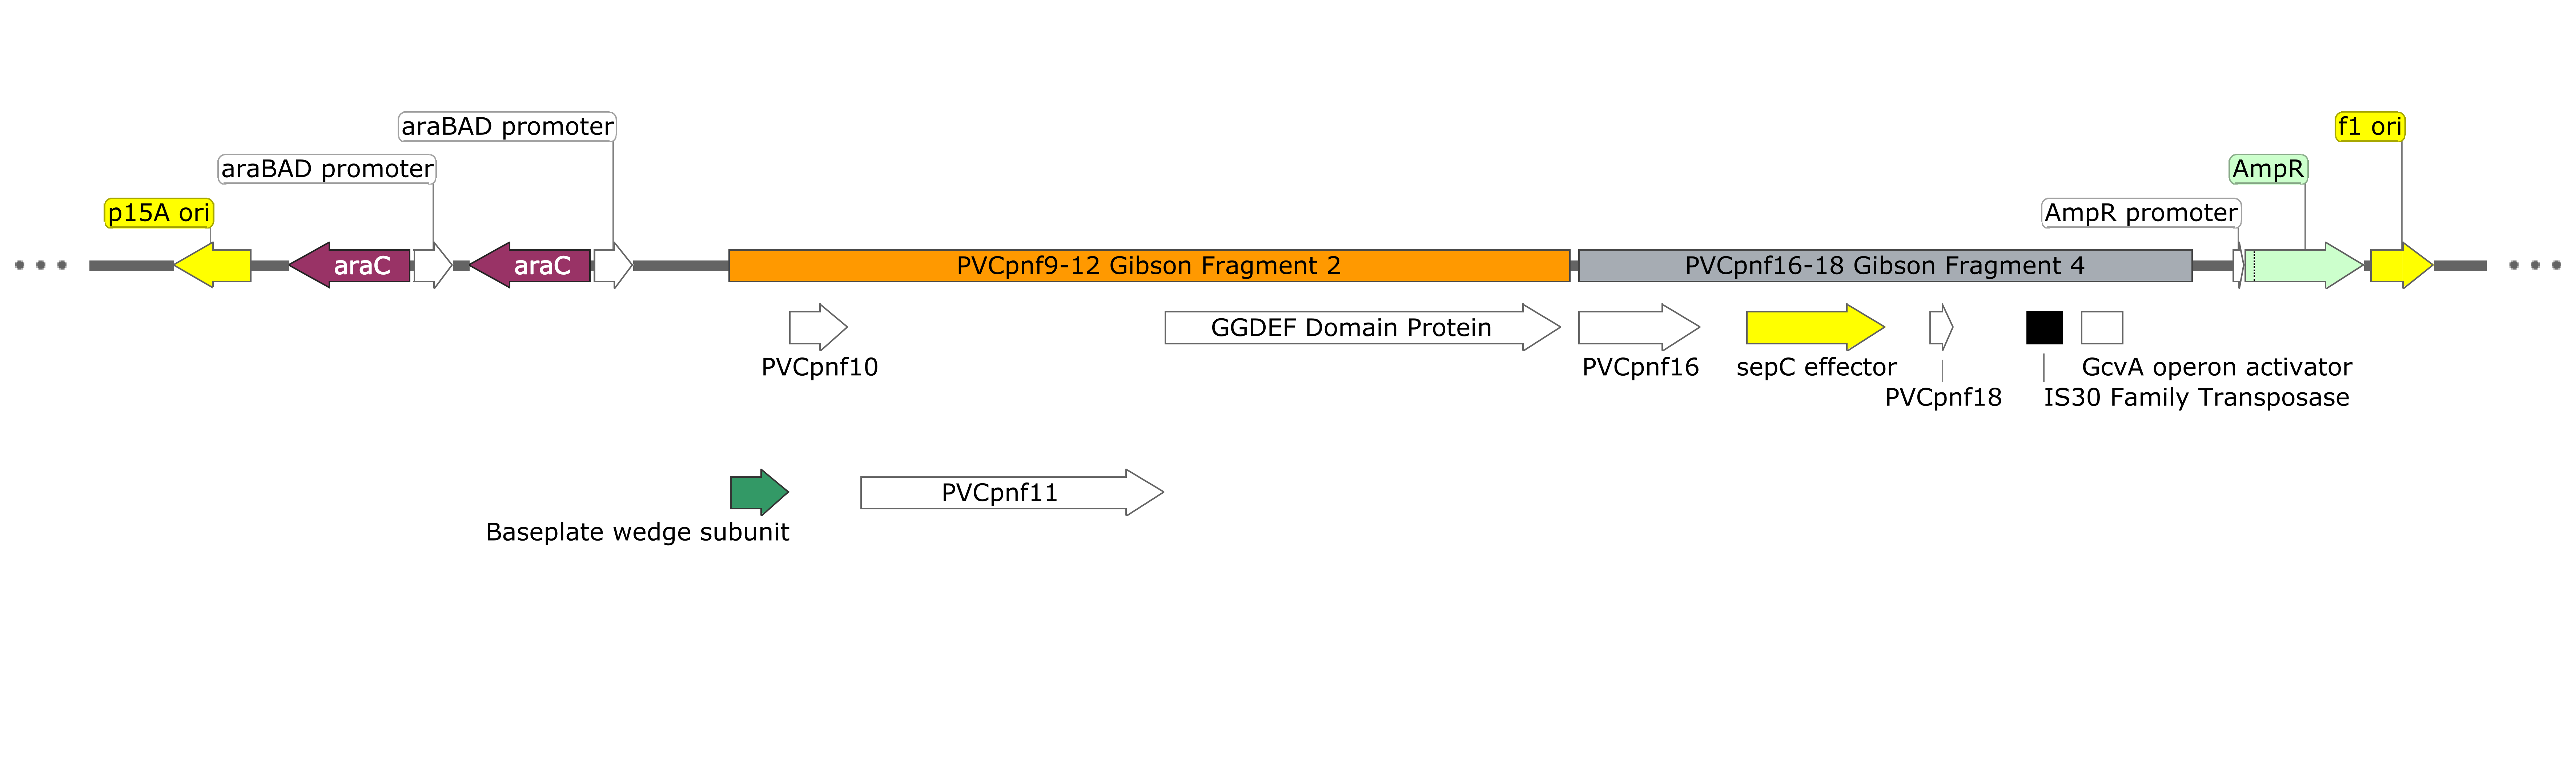
\includegraphics[width=\textwidth, clip, trim={0 140 0 65}]{/Users/joehealey/Documents/Warwick/PhD/Thesis/chapters/chapter6/img/GibsonD_bestcontigMap.png}
    \captionsetup{singlelinecheck=off, justification=centering, font=footnotesize, aboveskip=10pt}
    \caption{}
  \end{subfigure}
  
  \begin{subfigure}{\textwidth}
    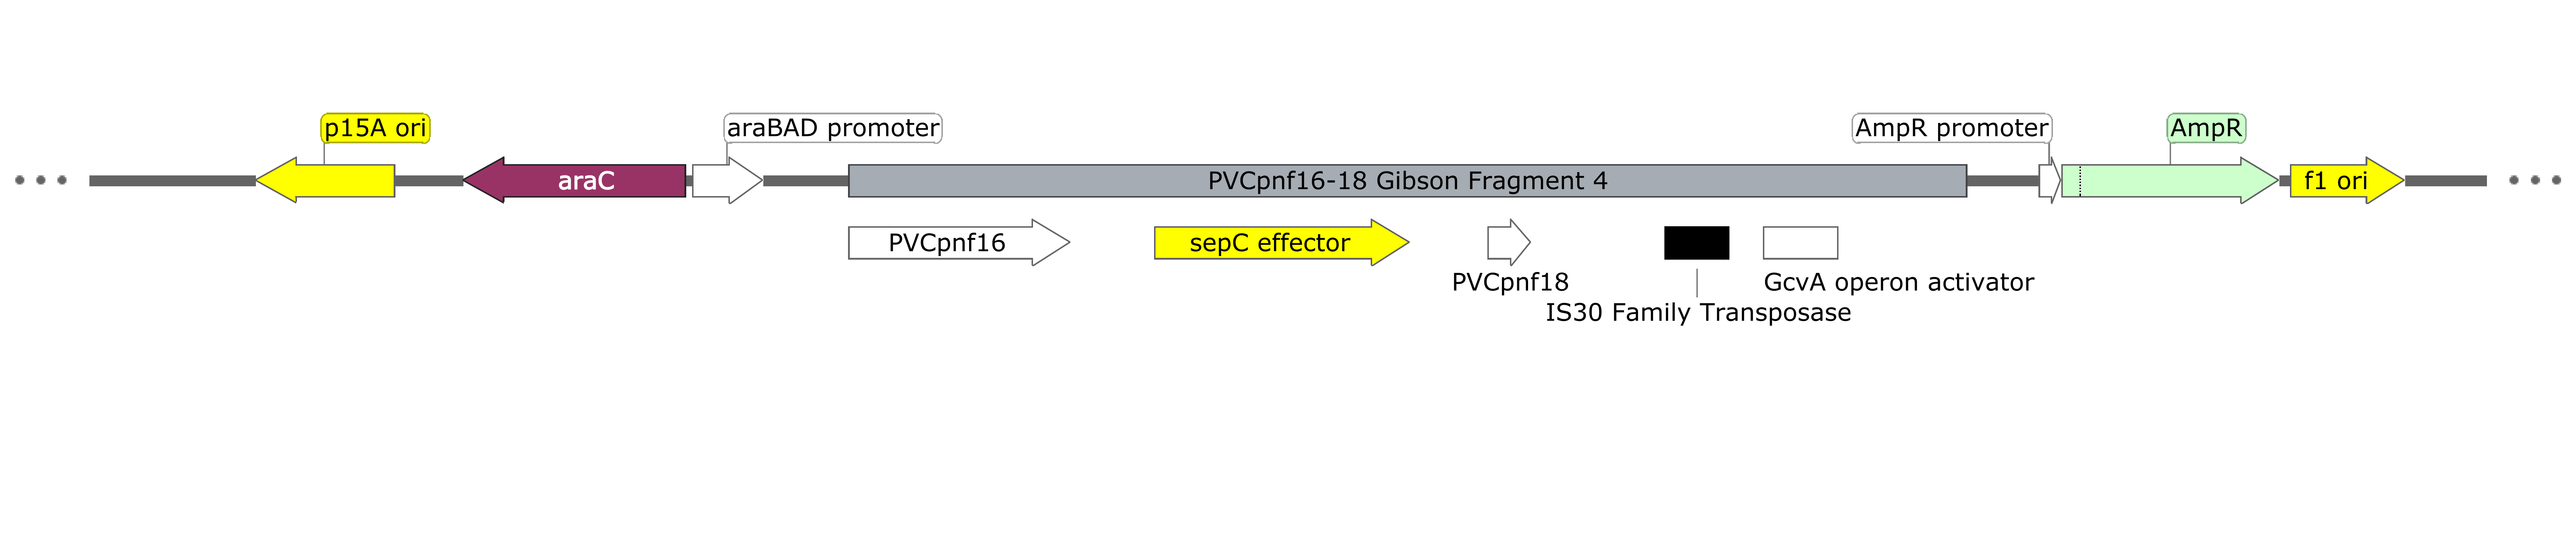
\includegraphics[width=\textwidth, clip, trim={0 50 0 65}]{/Users/joehealey/Documents/Warwick/PhD/Thesis/chapters/chapter6/img/GibsonC_bestcontigMap.png}
    \captionsetup{singlelinecheck=off, justification=centering, font=footnotesize, aboveskip=10pt}
    \caption{}
  \end{subfigure}
    
    \captionsetup{singlelinecheck=off, justification=justified, font=footnotesize, aboveskip=10pt}
    \caption[Gibson constructs obtained]{\textsc{\normalsize Vector maps of obtained Gibson constructs} \vspace{0.1cm} \newline Vector maps for a selection of obtained Gibson constructs, assembled from short reads. Assemblies in various states of completeness were obtained, demonstrating that the overlaps, fragment lengths, and protocol used for Gibson assembly appears viable. \textbf{(A)} The construct scheme devised for the PVCpnf operon from ATCC43949. The operon was broken in to 4 fragments, ranging from $\approx$4-8 kb, so as to avoid interrupting CDSs, and these are colour coded, with the genes below. \textbf{(B)} A Gibson construct which successfully incorporated {\color{red}fragment 1} and {\color{gray}fragment 4}, but no middle fragments. It successfully incorporated the largest fragment. Fragment 4 appears easy to clone as it is recovered in all the constructs (and more not shown). \textbf{(C)} A Gibson construct which successfully incorporated {\color{orange}fragment 2} which has several unknown genes, and {\color{gray}fragment 4} again. No constructs have been found with Fragments 1 and 2 surprisingly. \textbf{(D)} A smaller Gibson construct which has captured only {\color{gray}fragment 4}. This was the most commonly recovered construct, which is a little surprising as it carries a toxin and a number of putative regulators/transposaes etc. Conspicuously absent from any recovered constructs is {\color{Green}fragment 3}.}
\label{gibsonvectors}
\end{figure}


Two key optimisations which increased colony recovery and fragment incorporation were a step-wise assembly process (rather than the `one-pot' process recommended - see \vref{gibson}), as well as DpnI treatment of vector backbone templates for PCR, which drastically reduced the empty background.


Despite these optimisations however, it was not possible to obtain entirely complete assemblies, though several partial assemblies came close. \vref{gibsonvectors} shows a selection of the `most successful' constructs that were obtained. Interestingly though, these assemblies offer some clues as to why the PVCs appear recalcitrant to cloning.

Specifically, the cloning approach was able to recover an example of all of the PVC fragments that were cloned (see \vref{gibsonidealmap}), with the exception of fragment 3 (green), and possible reasons are explored in the discussion.


\subsection{Population heterogeneity in PVC activity}\label{heterogeneity}
A pre-existing hypothesis for the manner in which PVCs are deployed was that the populations may demonstrate extreme variability/heterogeneity, as is often the case with other aspects of \emph{Photorhabdus} physiology. In order to investigate this further, a selection of PVC operons from both \Plum{} and \Pasy{} were chosen to have their promoters cloned in to fusions with GFP. Briefly, the promoterless GFP bearing plasmid pGAG had been previously derivatised by the lab to remove the ribosome binding site and start codon of the GFP so that full promoter region fusions could be made. Primers were then designed to incorporate $\approx$500 bp upstream of 4 PVC operons, and the first 5 amino acids of each PVC1 locus from both \Plum{} and \Pasy, thus reconstituting the now fused GFP coding sequence and ensuring a reliable fusion. Since all the constructs follow the same basic format, \vref{reportermaps} shows the map of the multiple cloning site for a single example. Vector descriptions and primers can be found in \vref{methods}.


\begin{figure}[h]
    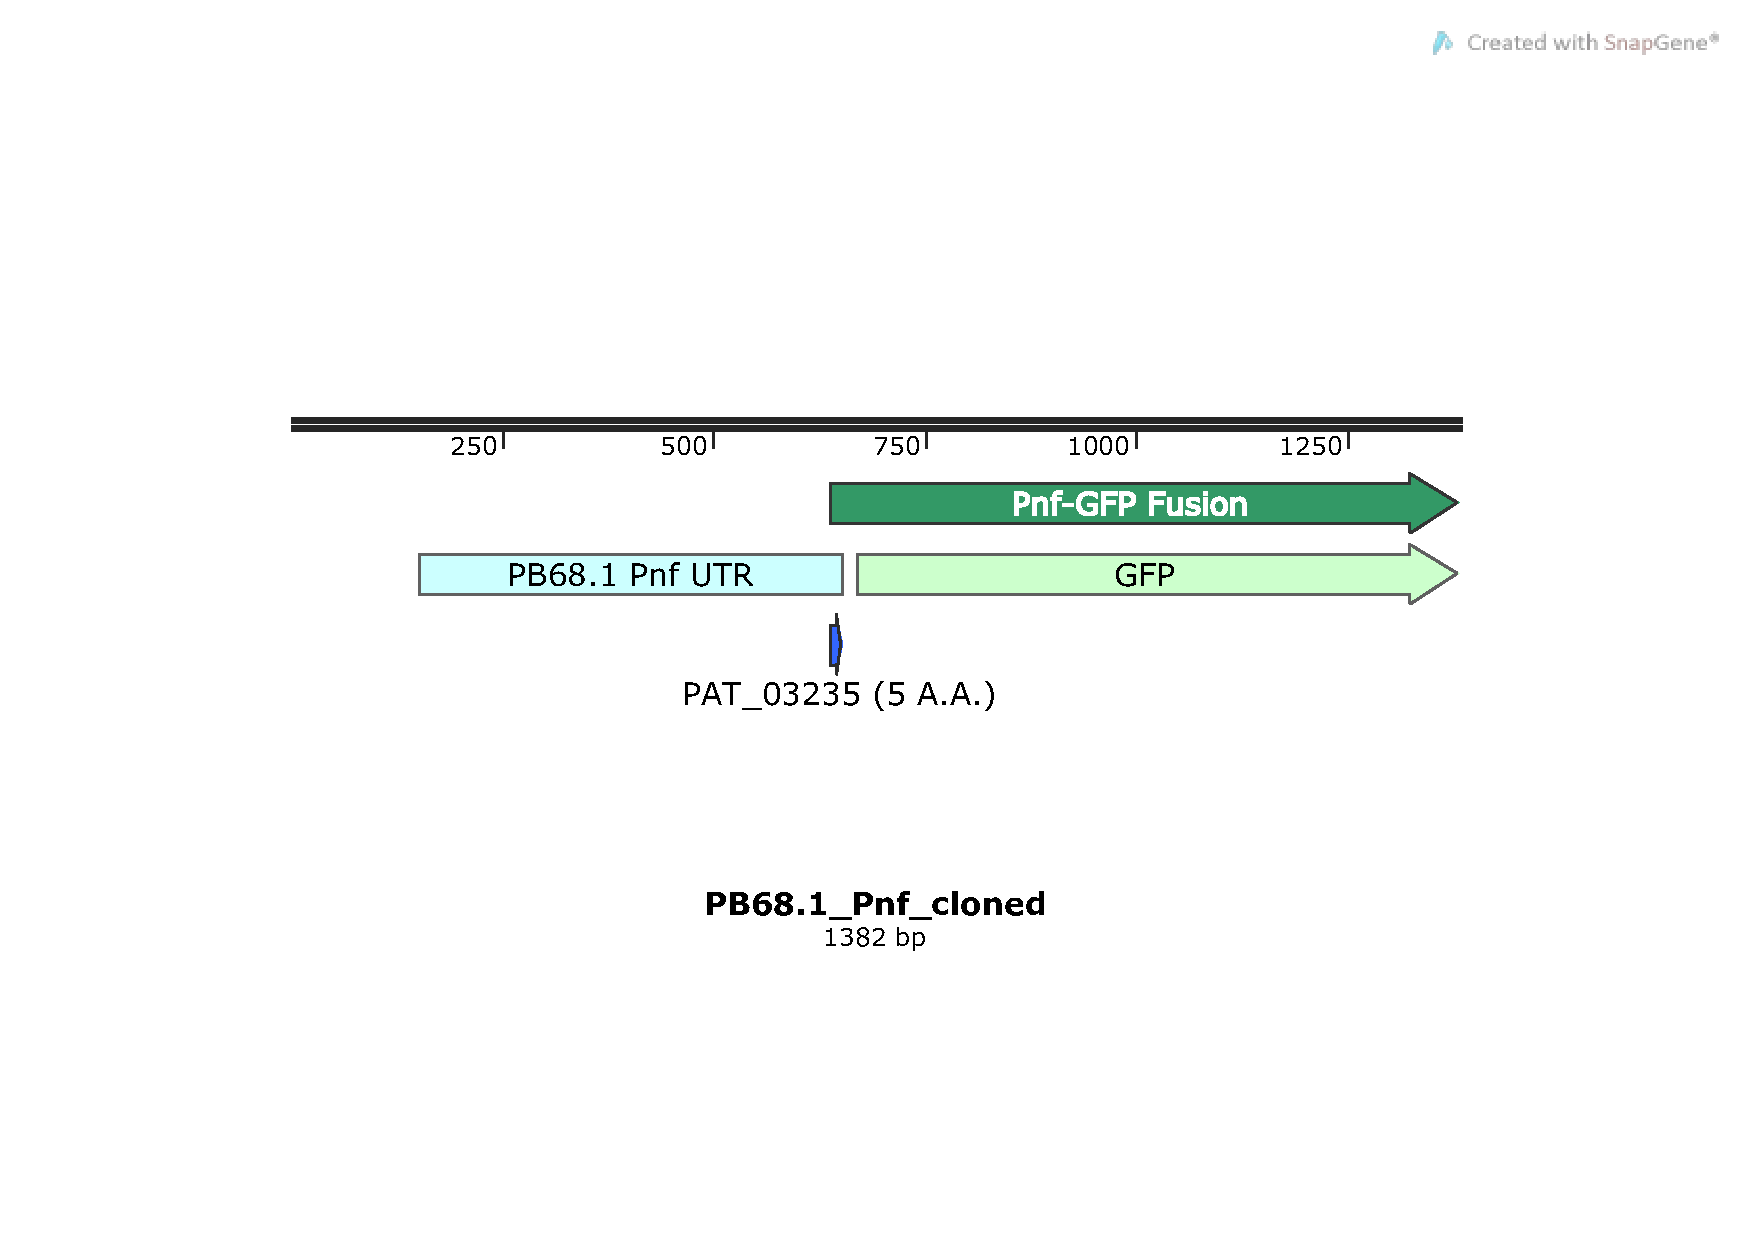
\includegraphics[width=\textwidth, clip, trim={82 240 82 200 }]{/Users/joehealey/Documents/Warwick/PhD/Thesis/chapters/chapter6/img/Pnf_cloned_Map.pdf}
    \captionsetup{singlelinecheck=off, justification=justified, font=footnotesize, aboveskip=10pt}
    \caption[Example of promoter fusions for PVC operons]{\textsc{\normalsize The promoter region fused to GFP for \Pasy{} PB68.1 Pnf in pAGAG} \vspace{0.1cm} \newline The construct scheme for promoter fusions of PVC operons. pAGAG has the RBS and start codon for GFP removed, allowing it to be replaced with the full promoter region of various PVCs. In this example, $\approx$500 bases upstream of the ``pnf" PVC from the \Pasy{} strain PB68.1 is inserted in to the BamHI and KpnI sites of the vector, creating a fusion that also has a small linker of 5 amino acids, following on from the first 5 amino acids of the PVC first locus.}
\label{reportermaps}
\end{figure}




Images were captured on a Leica DMi-8 inverted epifluorescent microscope with a Hamamatsu Flash4 4K camera, under phase contrast and GFP fluorescent channels. Due to heterogeneity in the sample prep on agar pad-based slides, some images were darker than others. Consequently, images have been postprocessed to normalise their intensities to a control reference image which had an acceptable grey intensity for reproduction clarity. Images have also had their colour depth reduced, as well as being downsampled to 35 pixels per inch, from 72 (to reduce image file size).

4 images per slide/time point are shown to give a representative sampling of the slide as best as possible. There is a key to the semi-quantitative fluorescence levels below each column. In a departure from the sequence discussed in the chapters so far, the \emph{P. asymbiotica} strain used here is not the `model' strain ATCC43949, but instead a Thai isolate denoted PB68.1. This was used as it is considerably easier to transform than the ATCC43949 strain, allowing for an \emph{P. asymbiotica} and a \Plum{} strain comparison.

The degree of fluorescence is scored based on the intensity seen in the stills captured, but also indirectly incorporates a dimension of time, as the semi-quantitative values that are given are also taking in to consideration the time taken to scan the slide and look for regions of interest. To be more explicit, if a slide was found with one or two extremely bright cells, but it took considerably longer to find those 2 cells amongst the population, that sample will be given a lower brightness score, reflecting the heterogeneity and scarcity of the fluorescent cells. A selection of `empty vector' controls, without promoters or GFP start codons are also shown, to demonstrate that it is not simply background activity.

% Separate input file for all the microscopy images due to size.
\begingroup
\renewcommand{\arraystretch}{0.8}%
\setlength{\tabcolsep}{0.3pt}
\begin{figure}[p]
\setkeys{Gin}{width=\linewidth}
\Huge
\begin{tabularx}{\textwidth}{CCCC}
\multicolumn{4}{p{\linewidth}}{\large \centering \textbf{\emph{P. luminescens} TT01 PVC ``Unit 1"}} \\
\hiderowcolors
& & & \\[-1.5ex]
\Large 2 Hours &\Large 5 Hours &\Large 24 Hours &\Large 72 Hours \\[1ex]

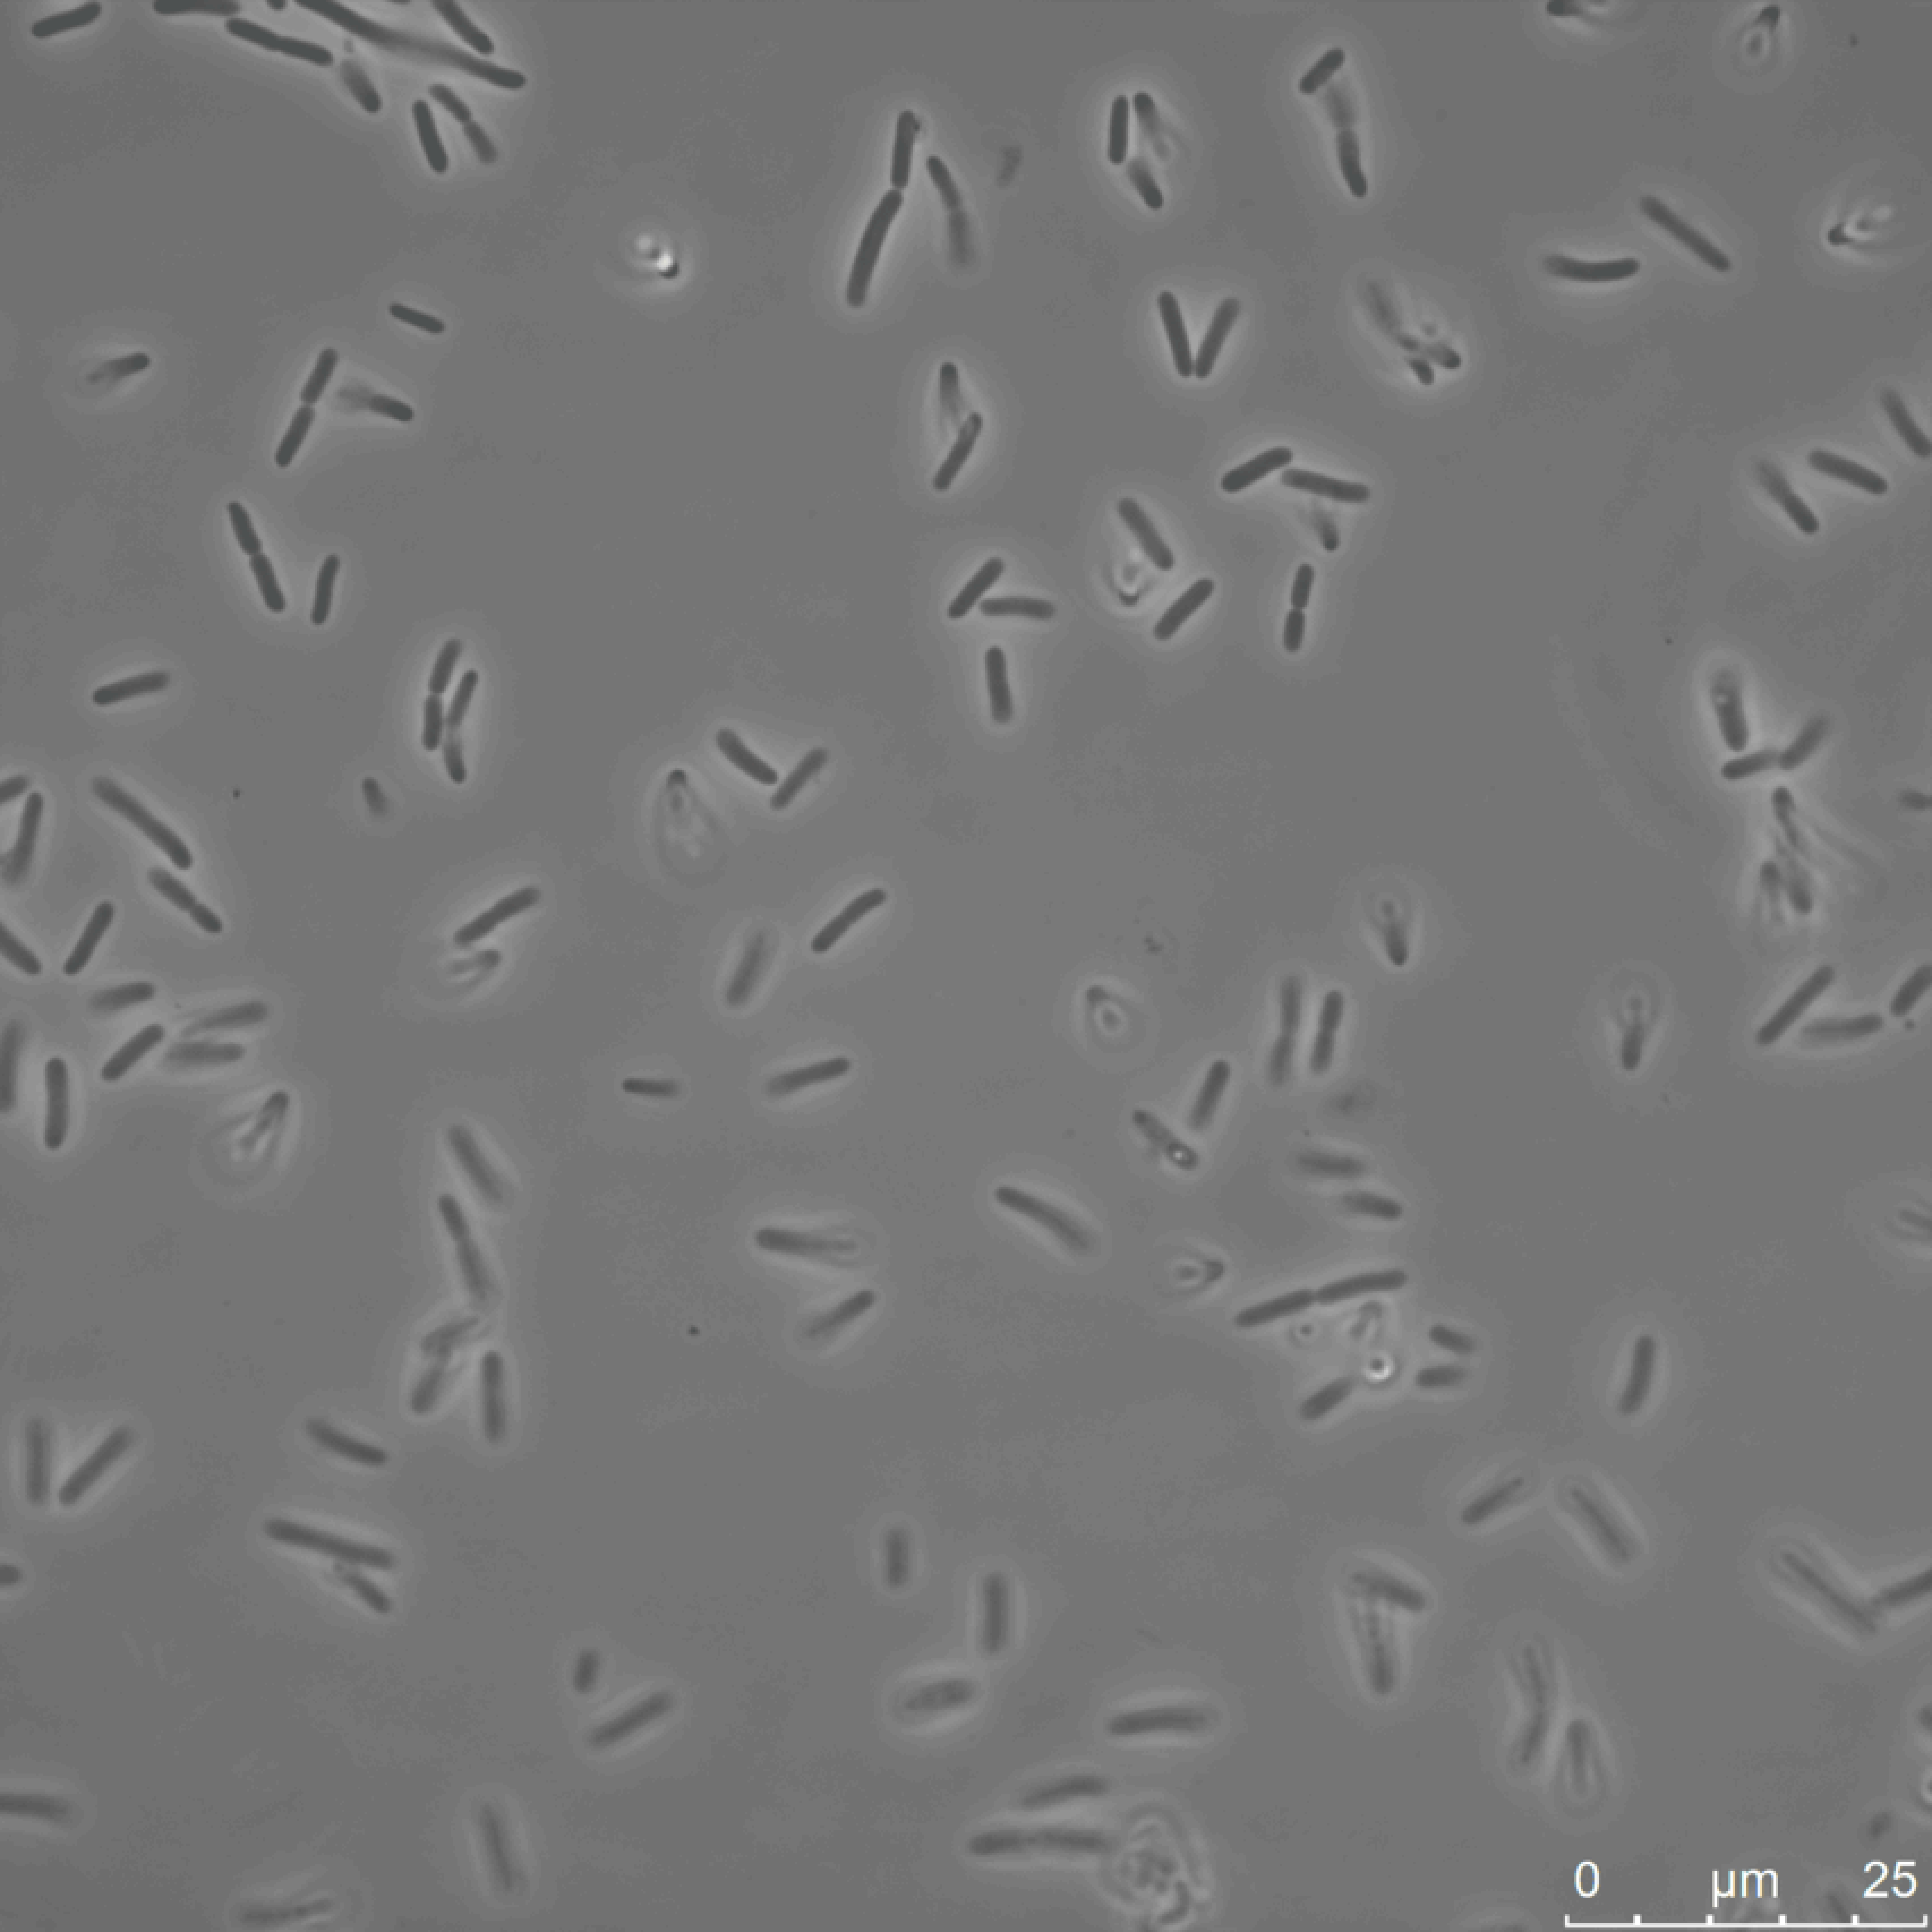
\includegraphics{TT01U1_1_NOGREEN-crunch-lighter-resample.pdf} &%
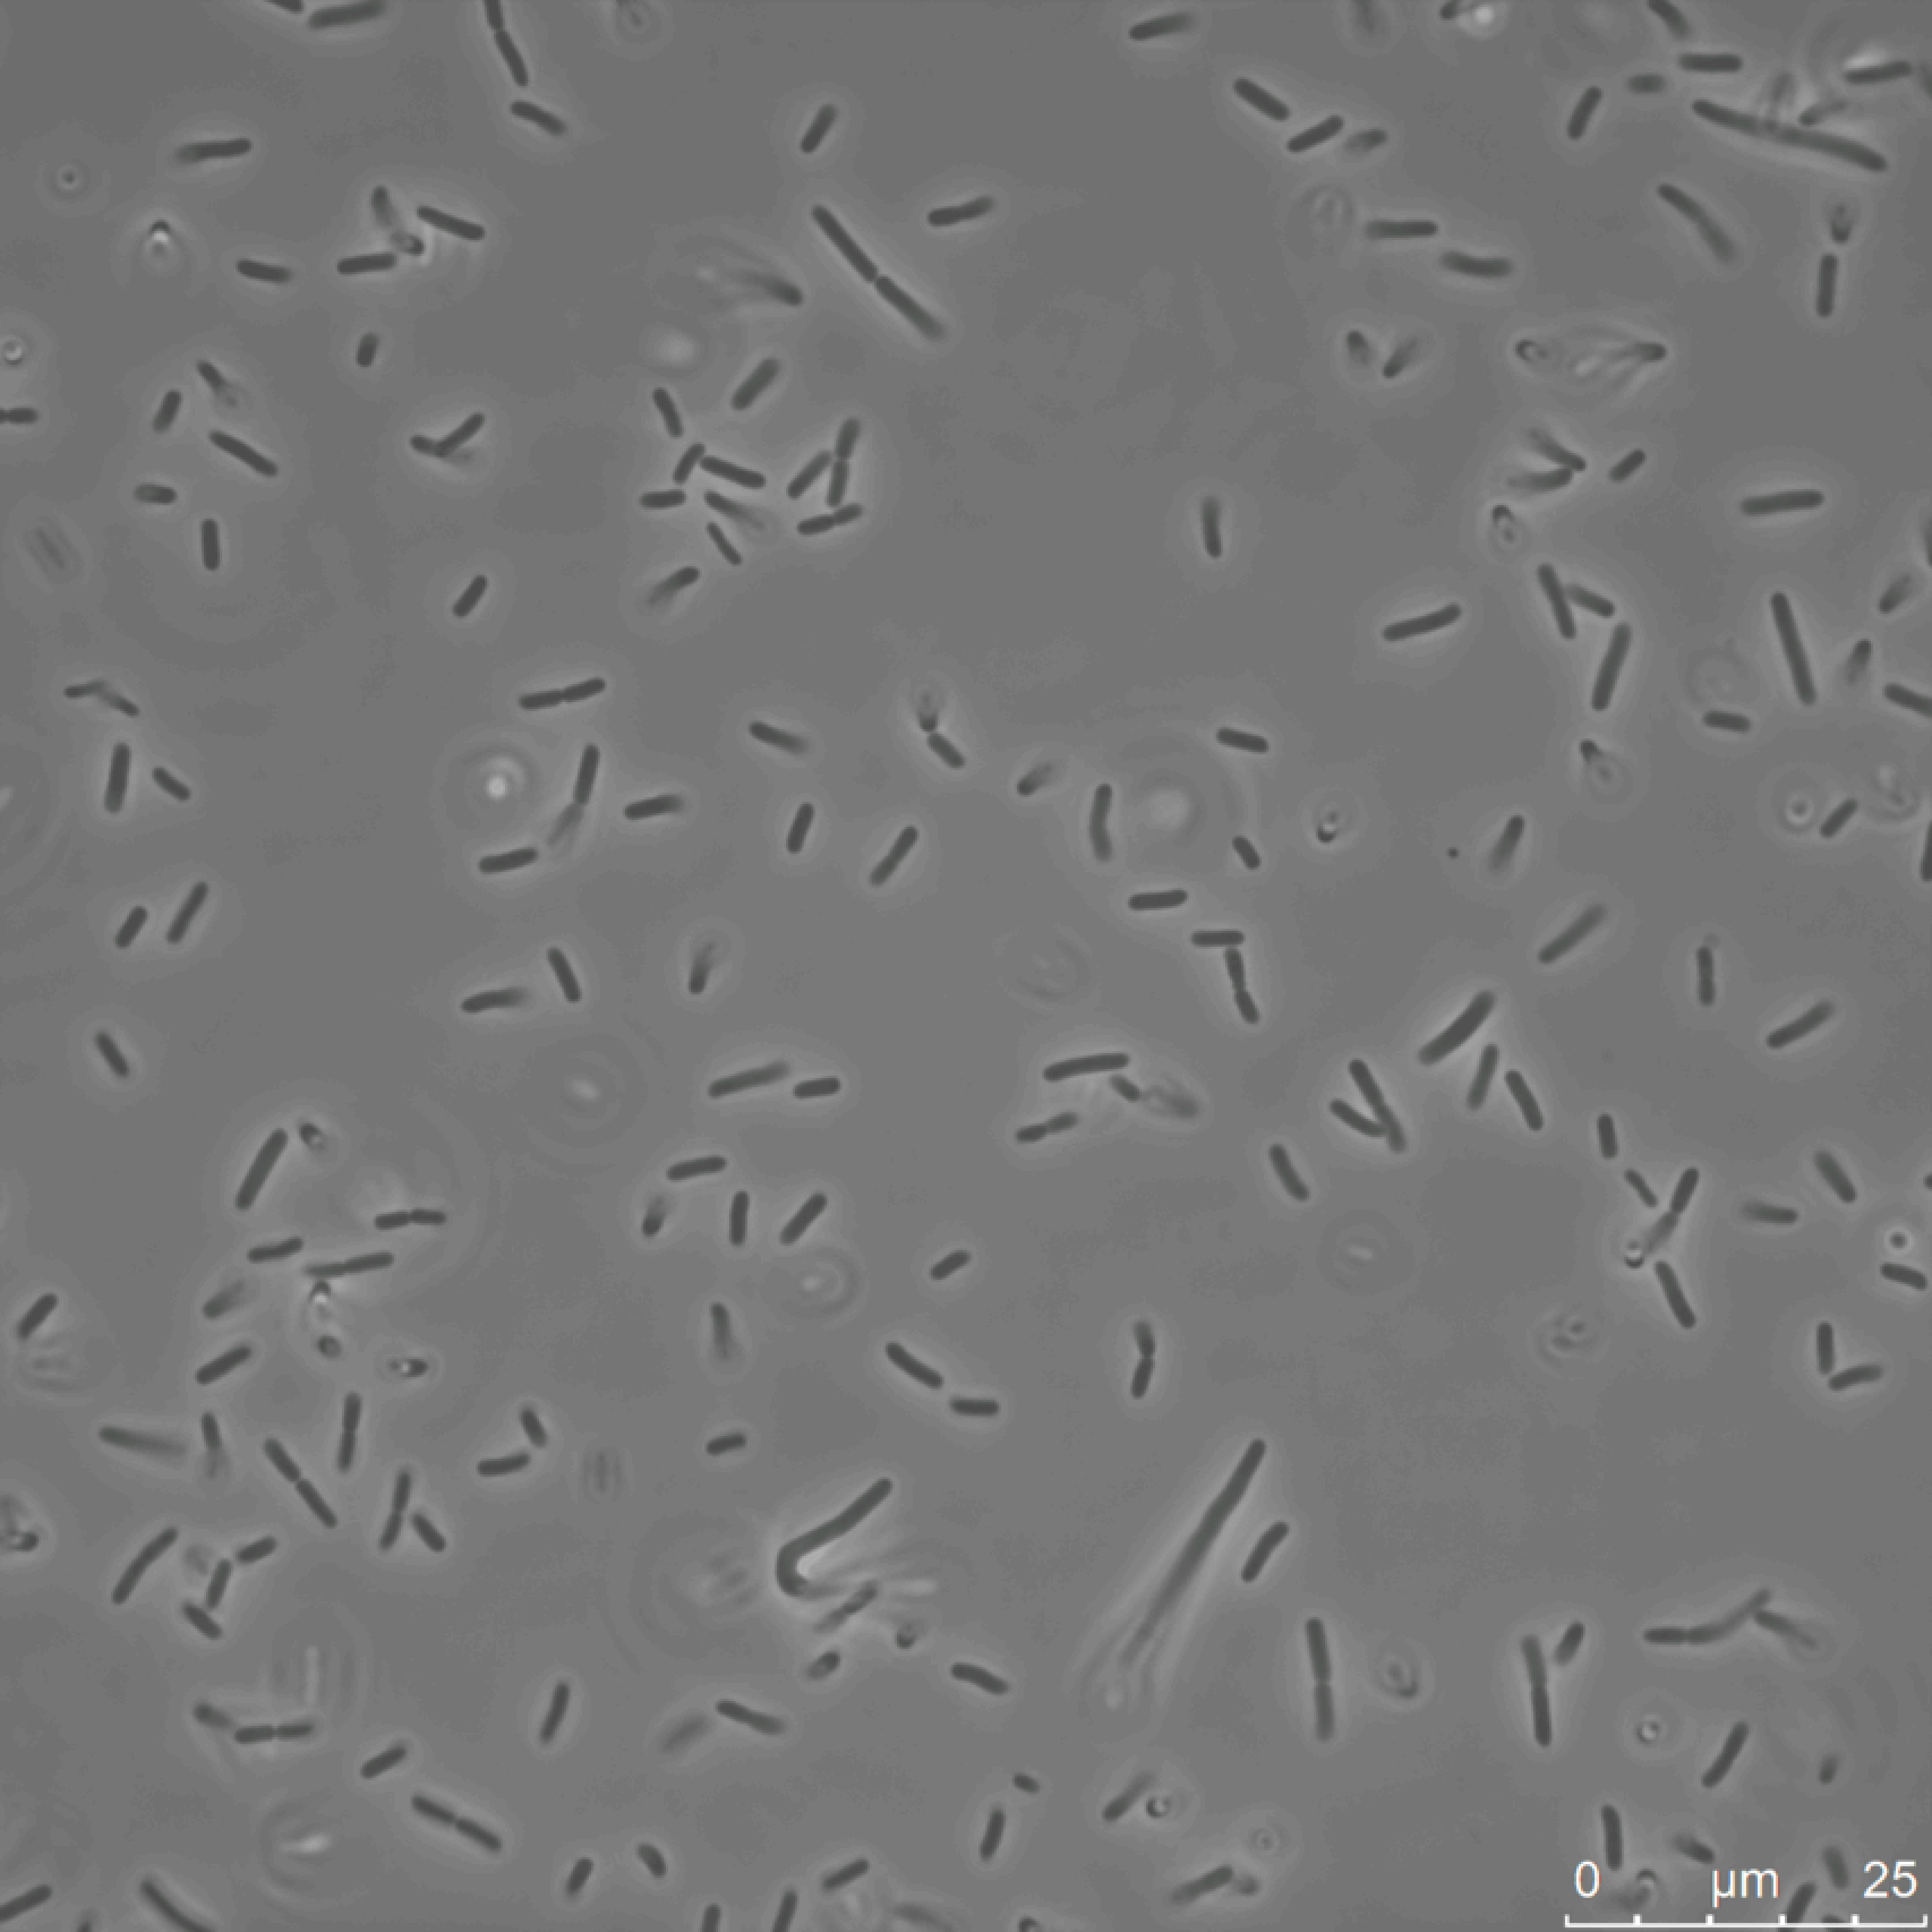
\includegraphics{TT01U1_5HR_5_LOWGREEN-crunch-lighter-resample.pdf} &%
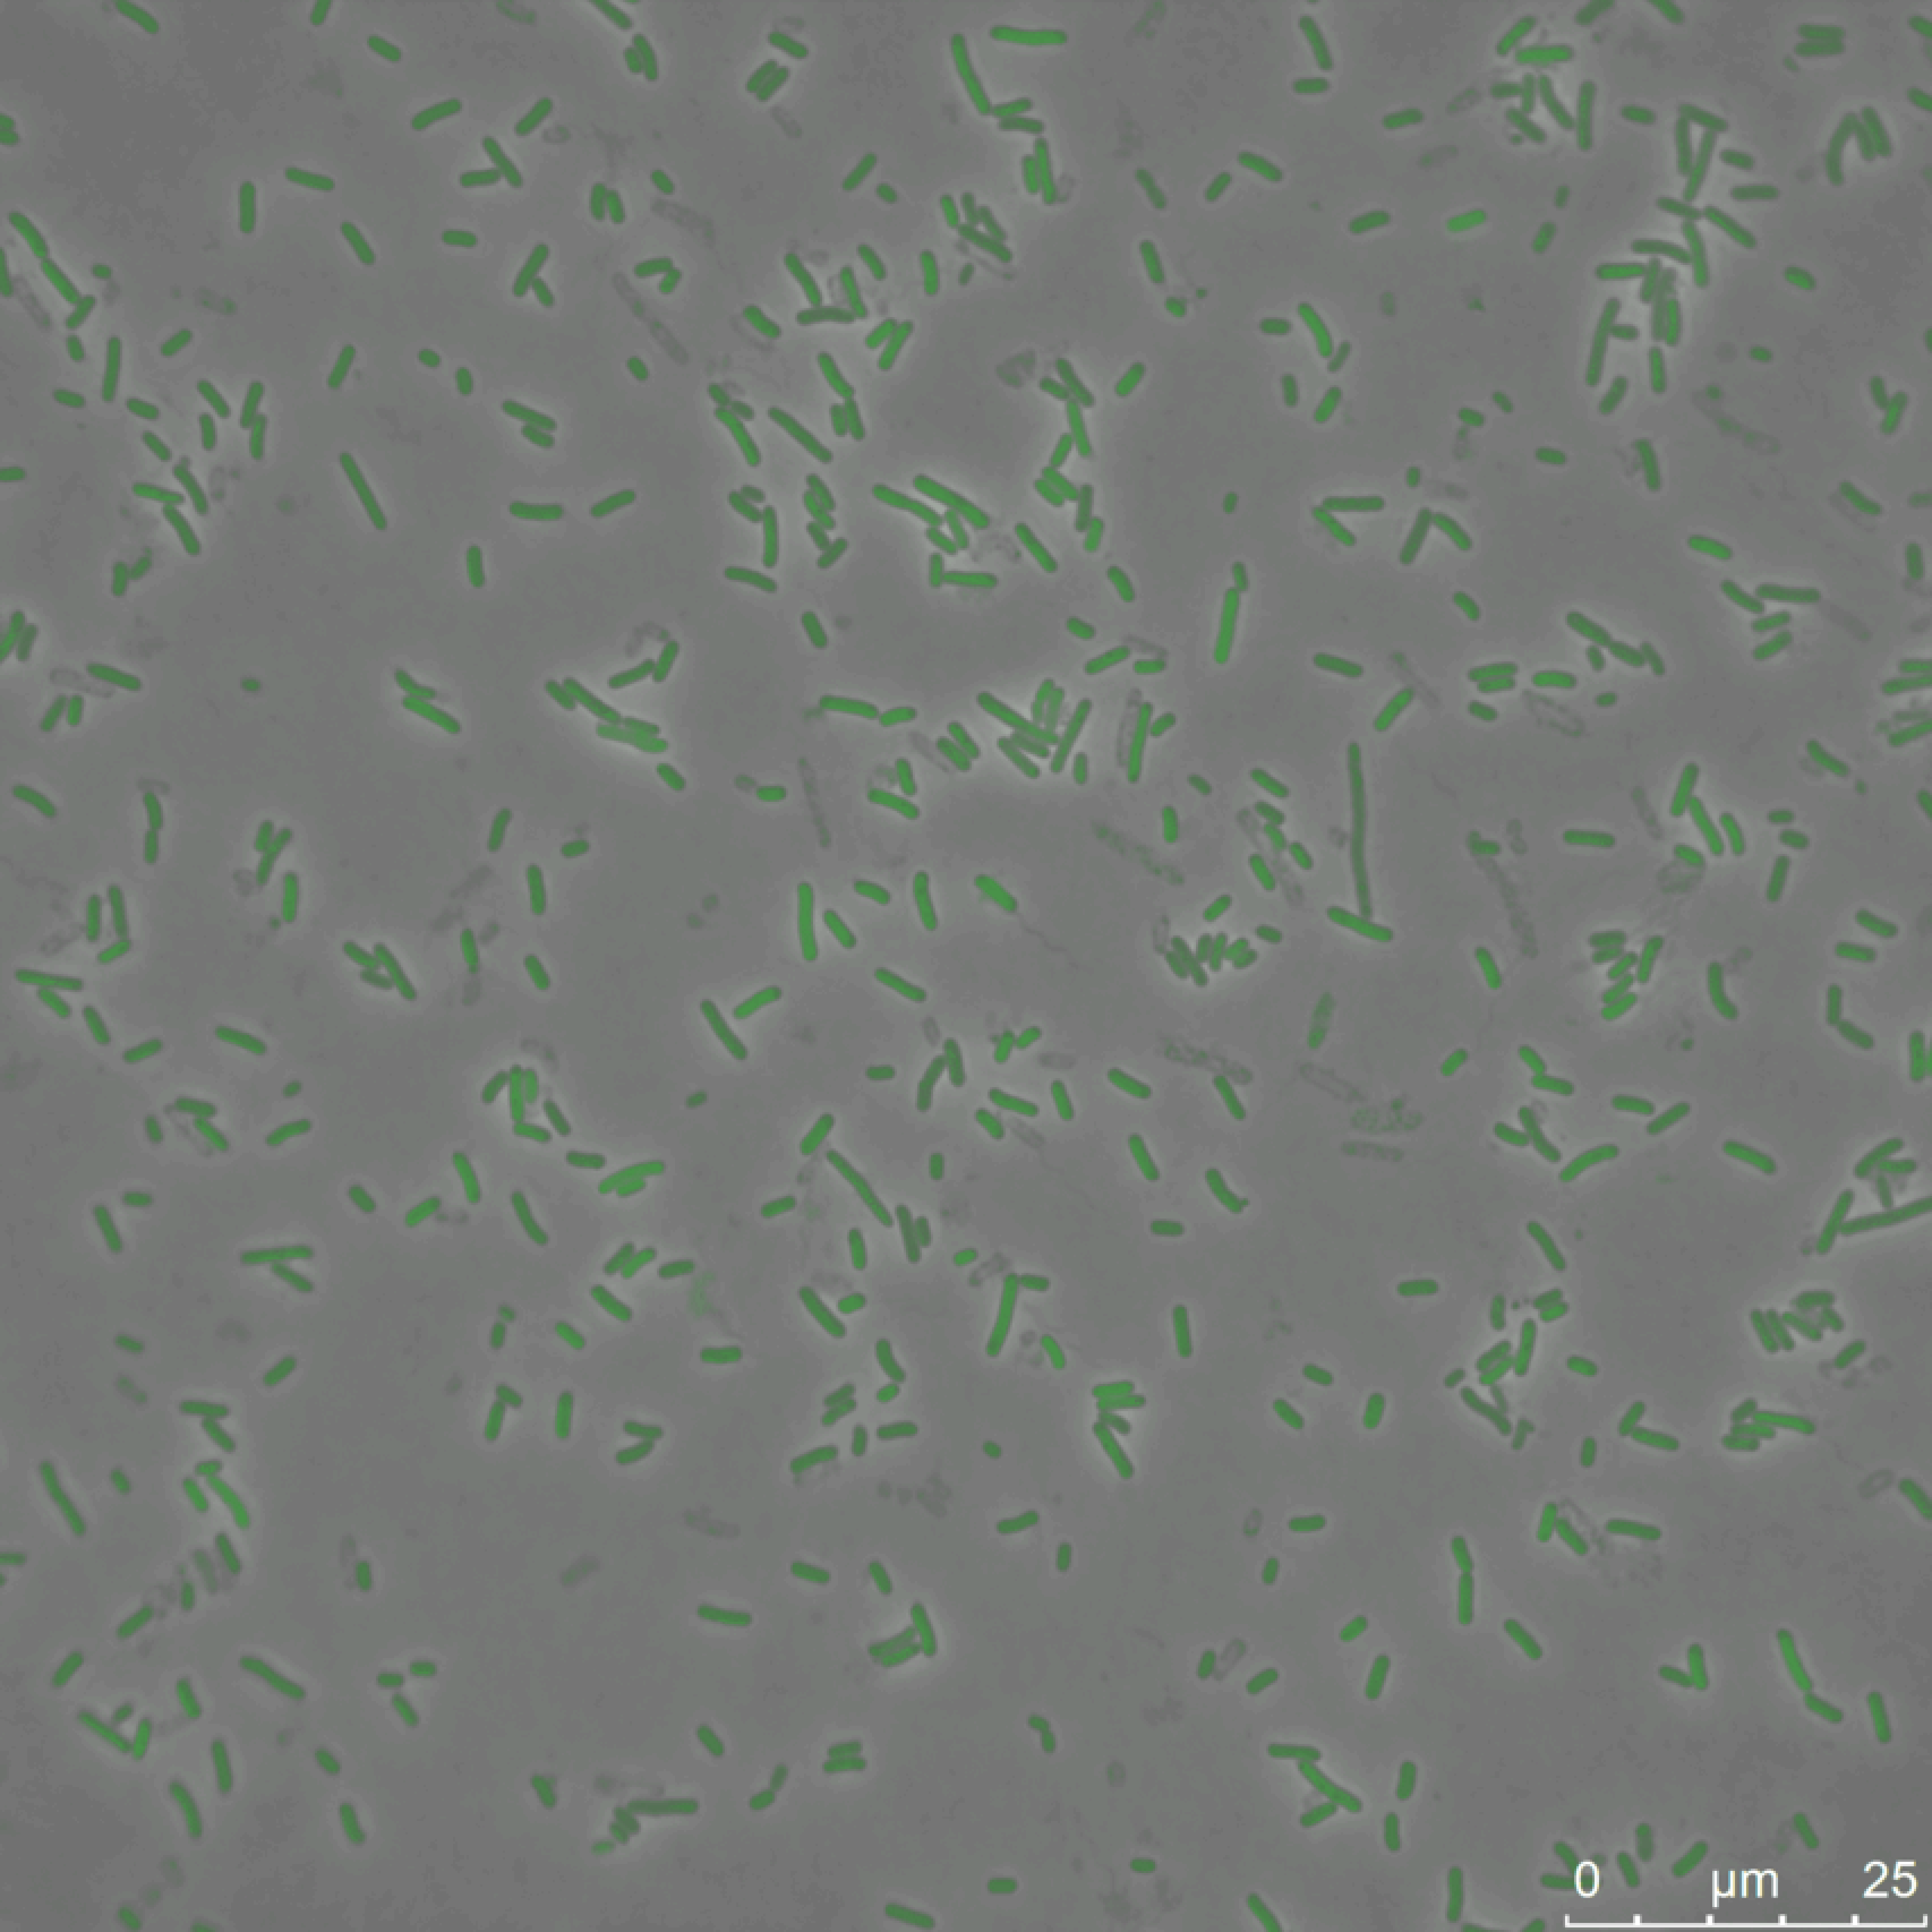
\includegraphics{TT01U1_24HR_1_GREEN-crunch-lighter-resample.pdf} &%
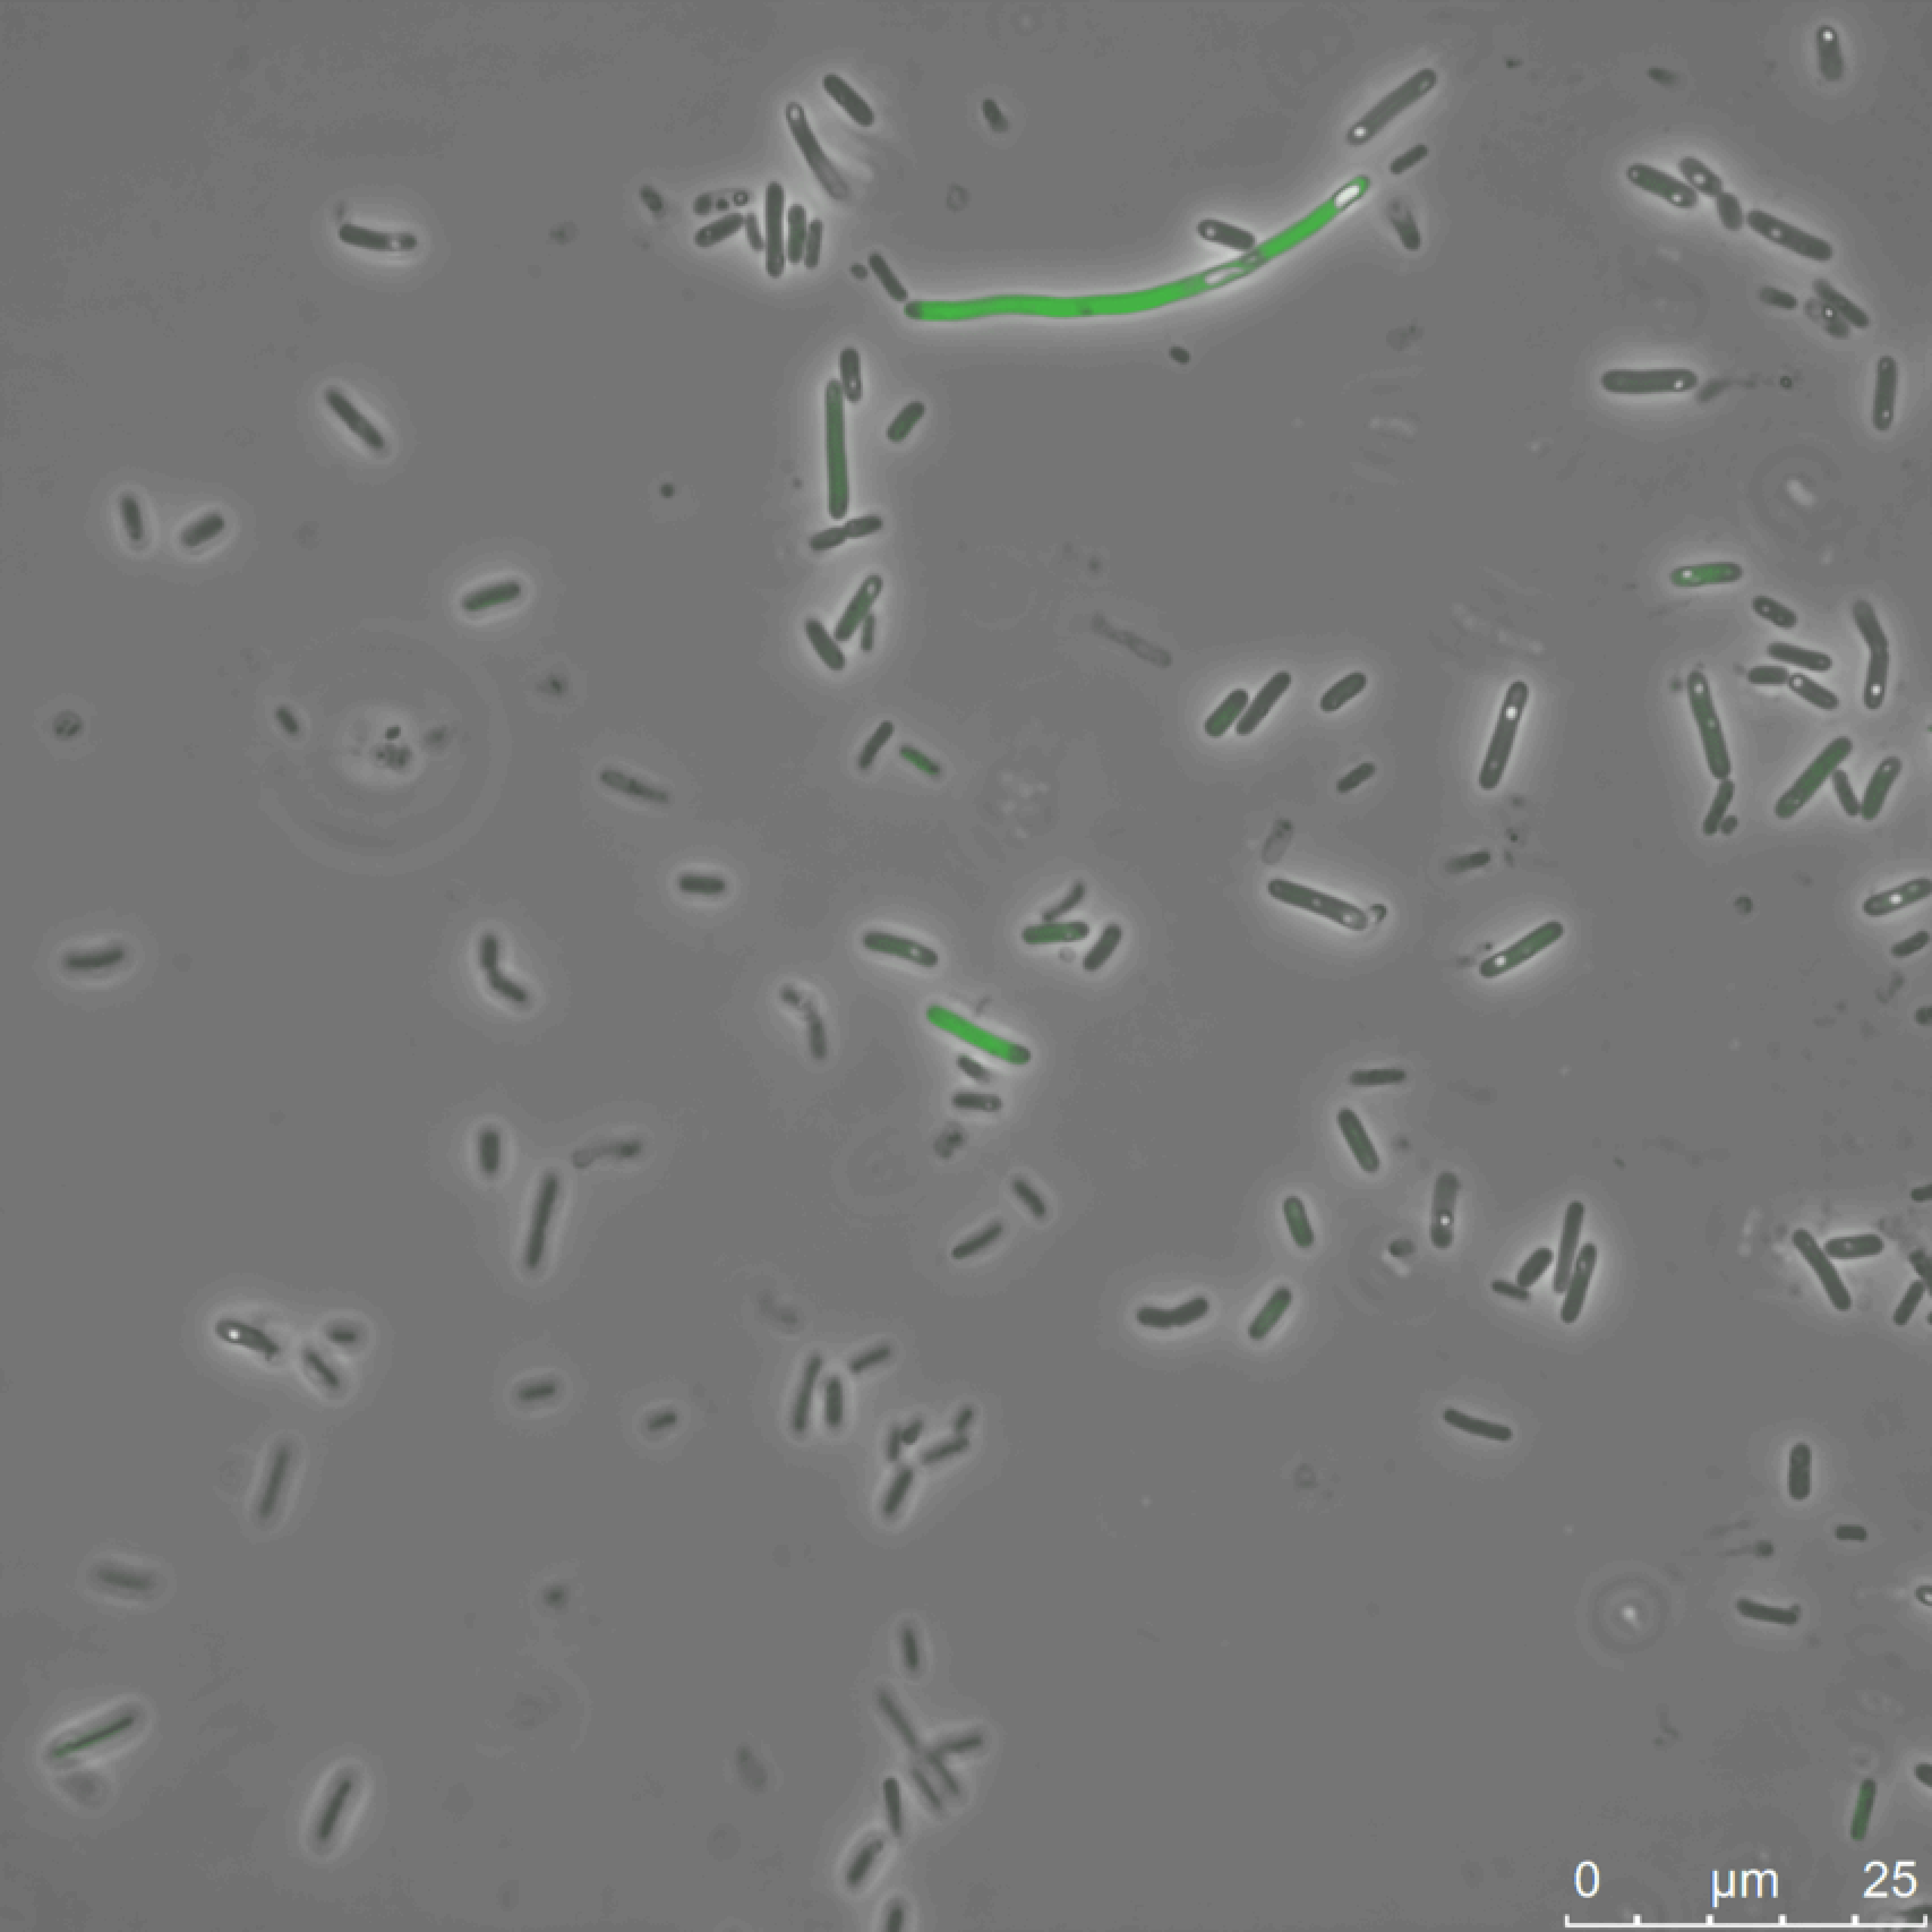
\includegraphics{TT01U1_72HR_1_GREEN-crunch-lighter-resample.pdf} \\[-0.5ex]

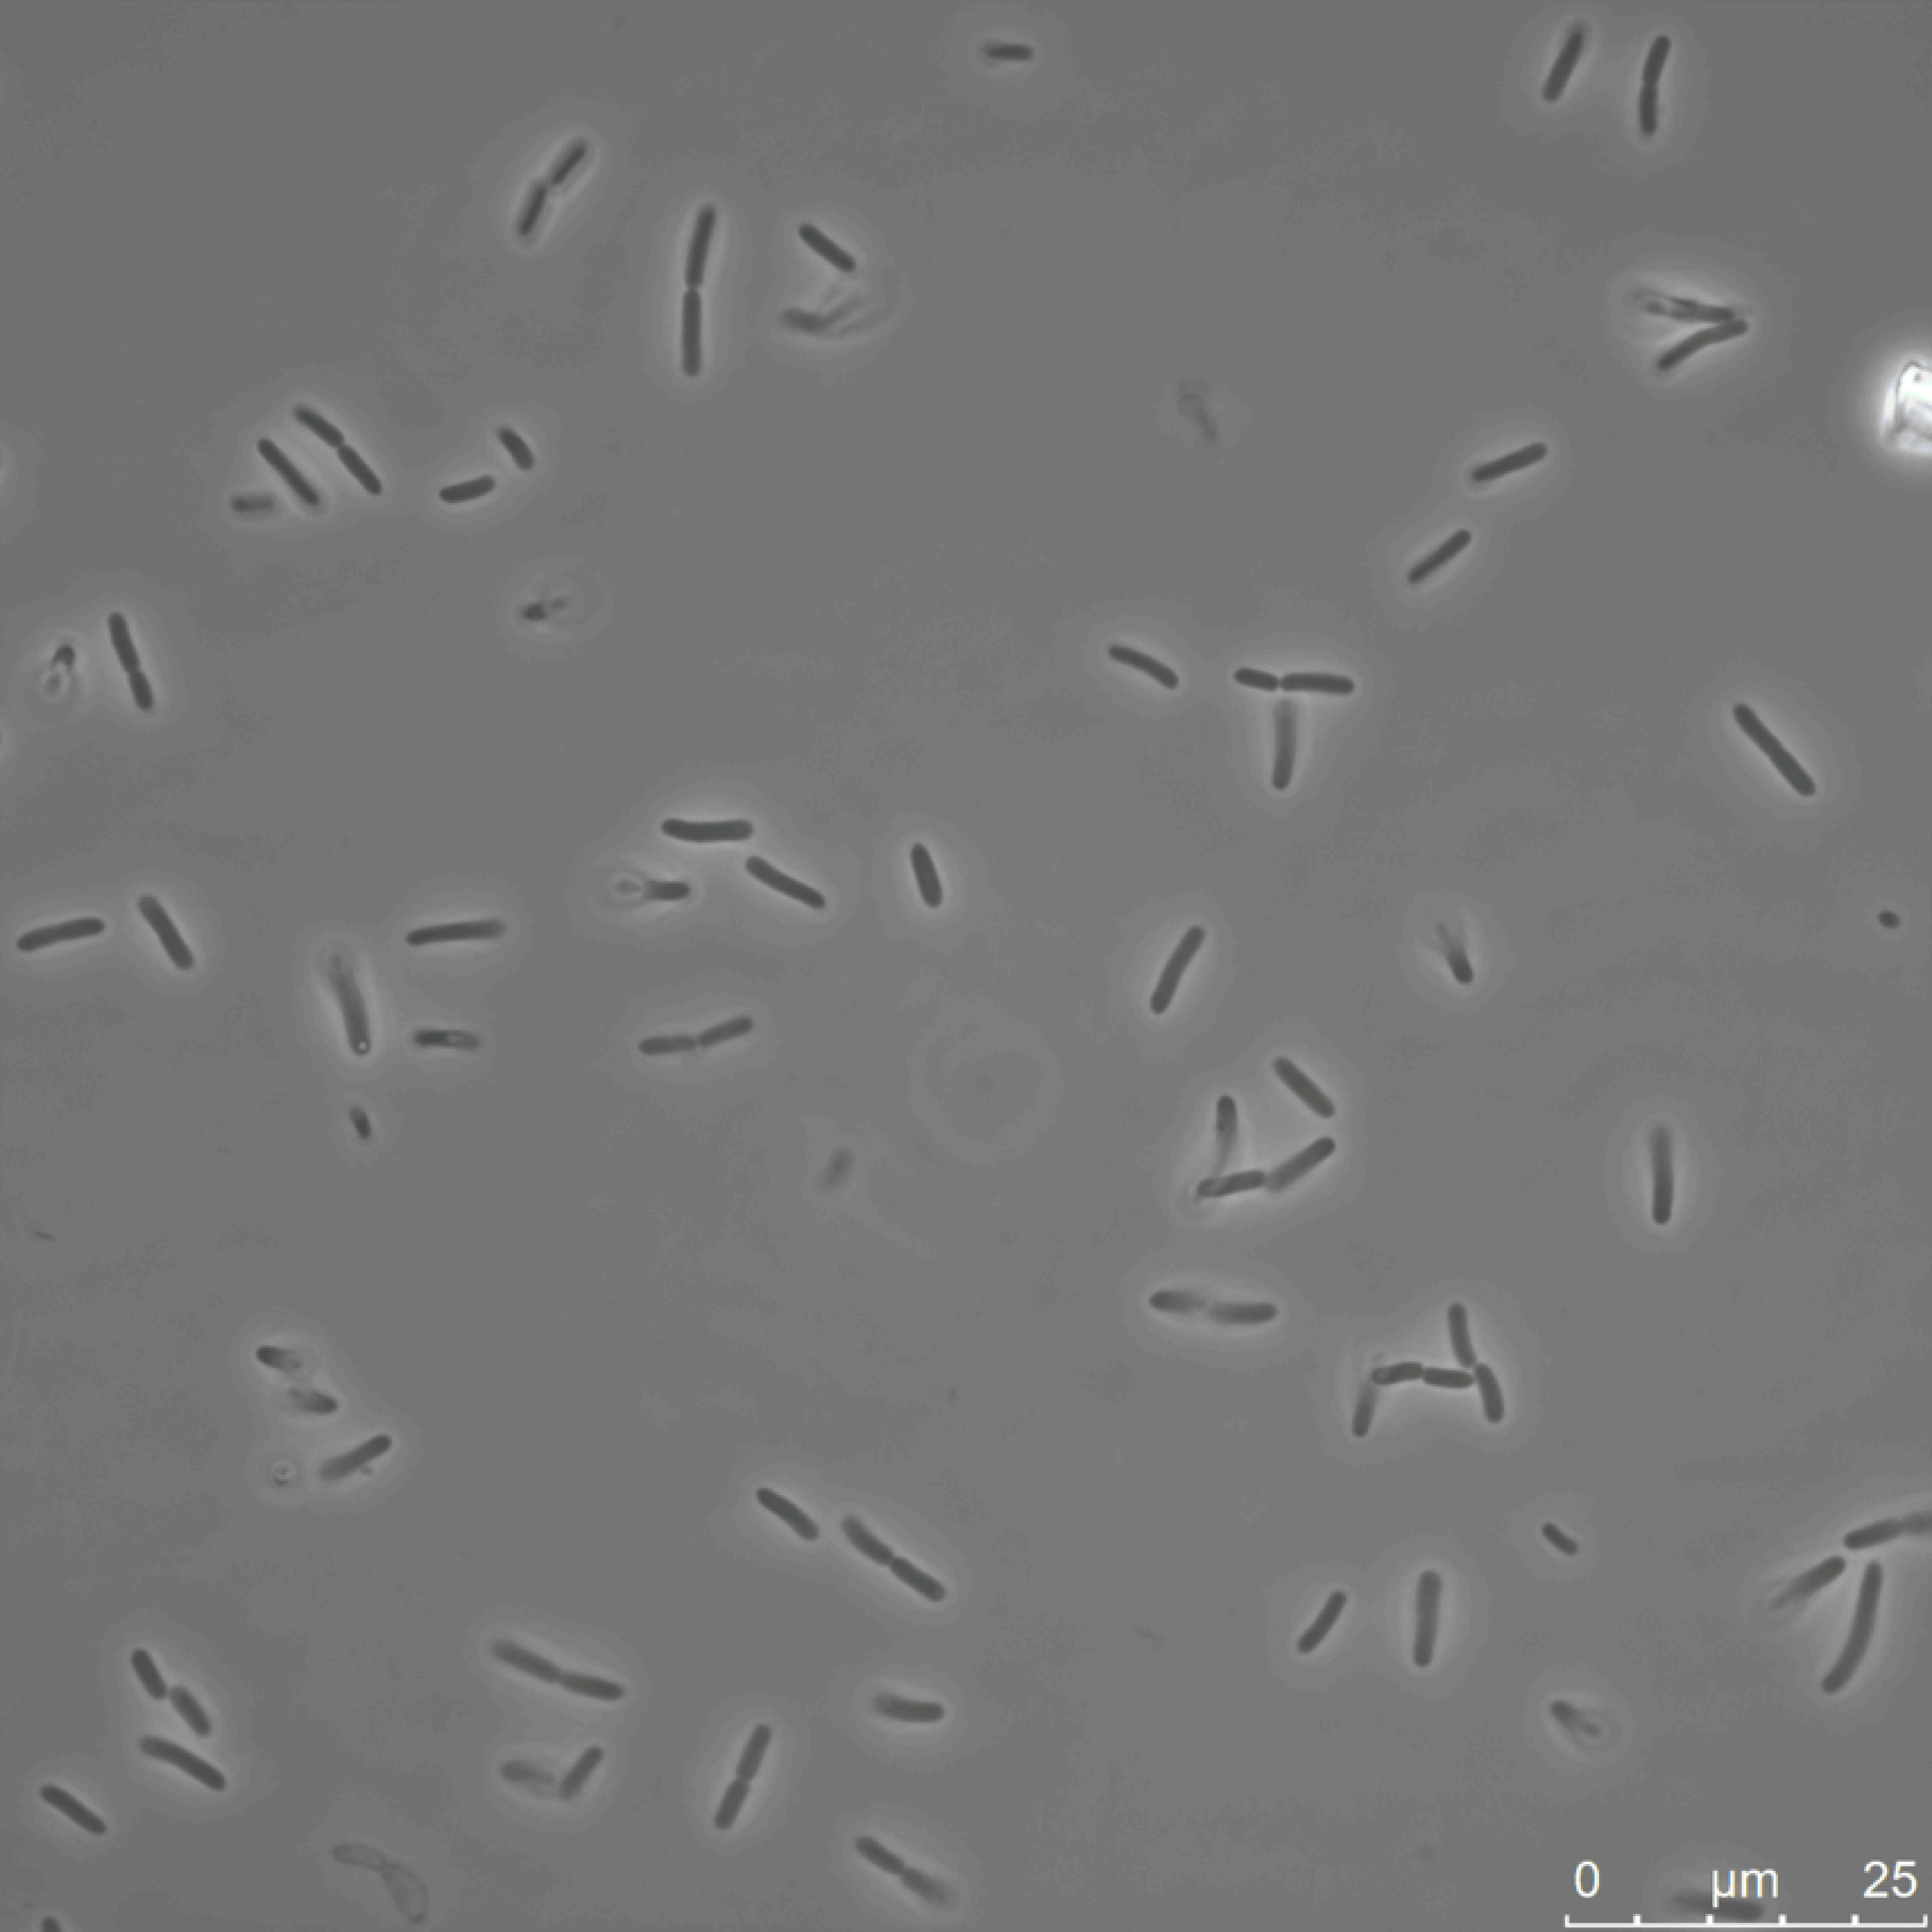
\includegraphics{TT01U1_2_NOGREEN-crunch-lighter-resample.pdf} &%
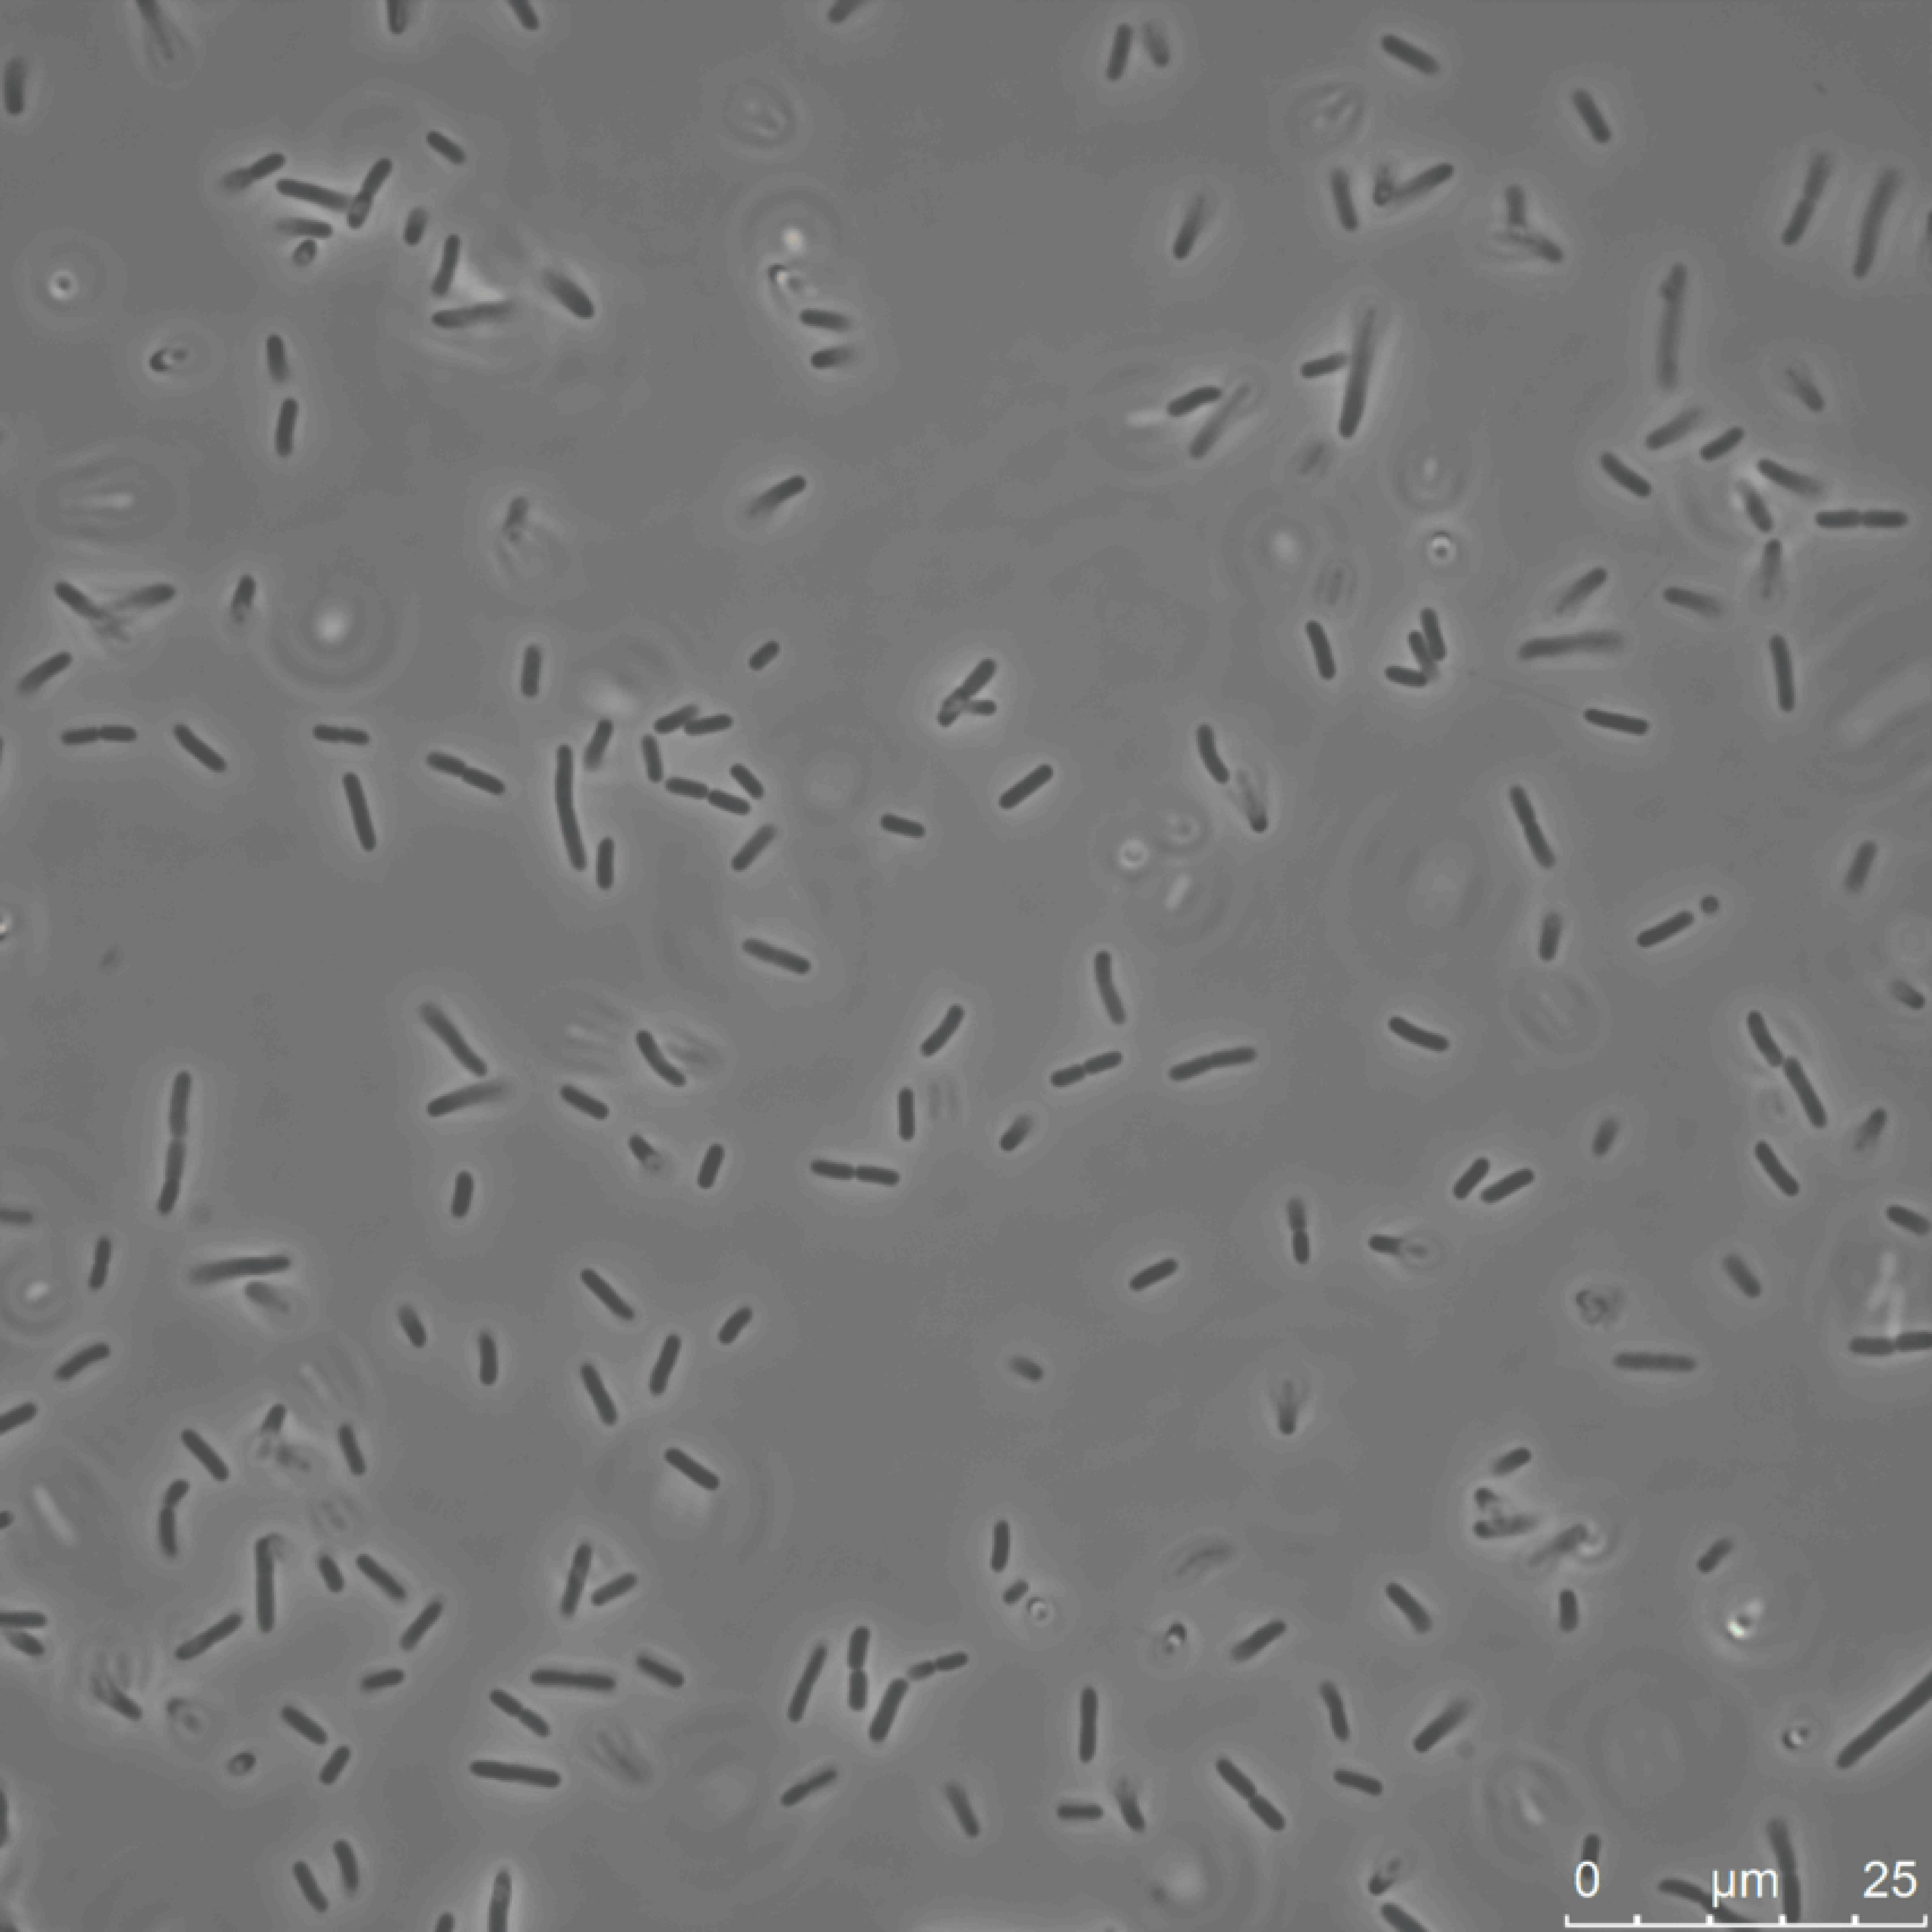
\includegraphics{TT01U1_5HR_2_NOGREEN-crunch-lighter-resample.pdf} &%
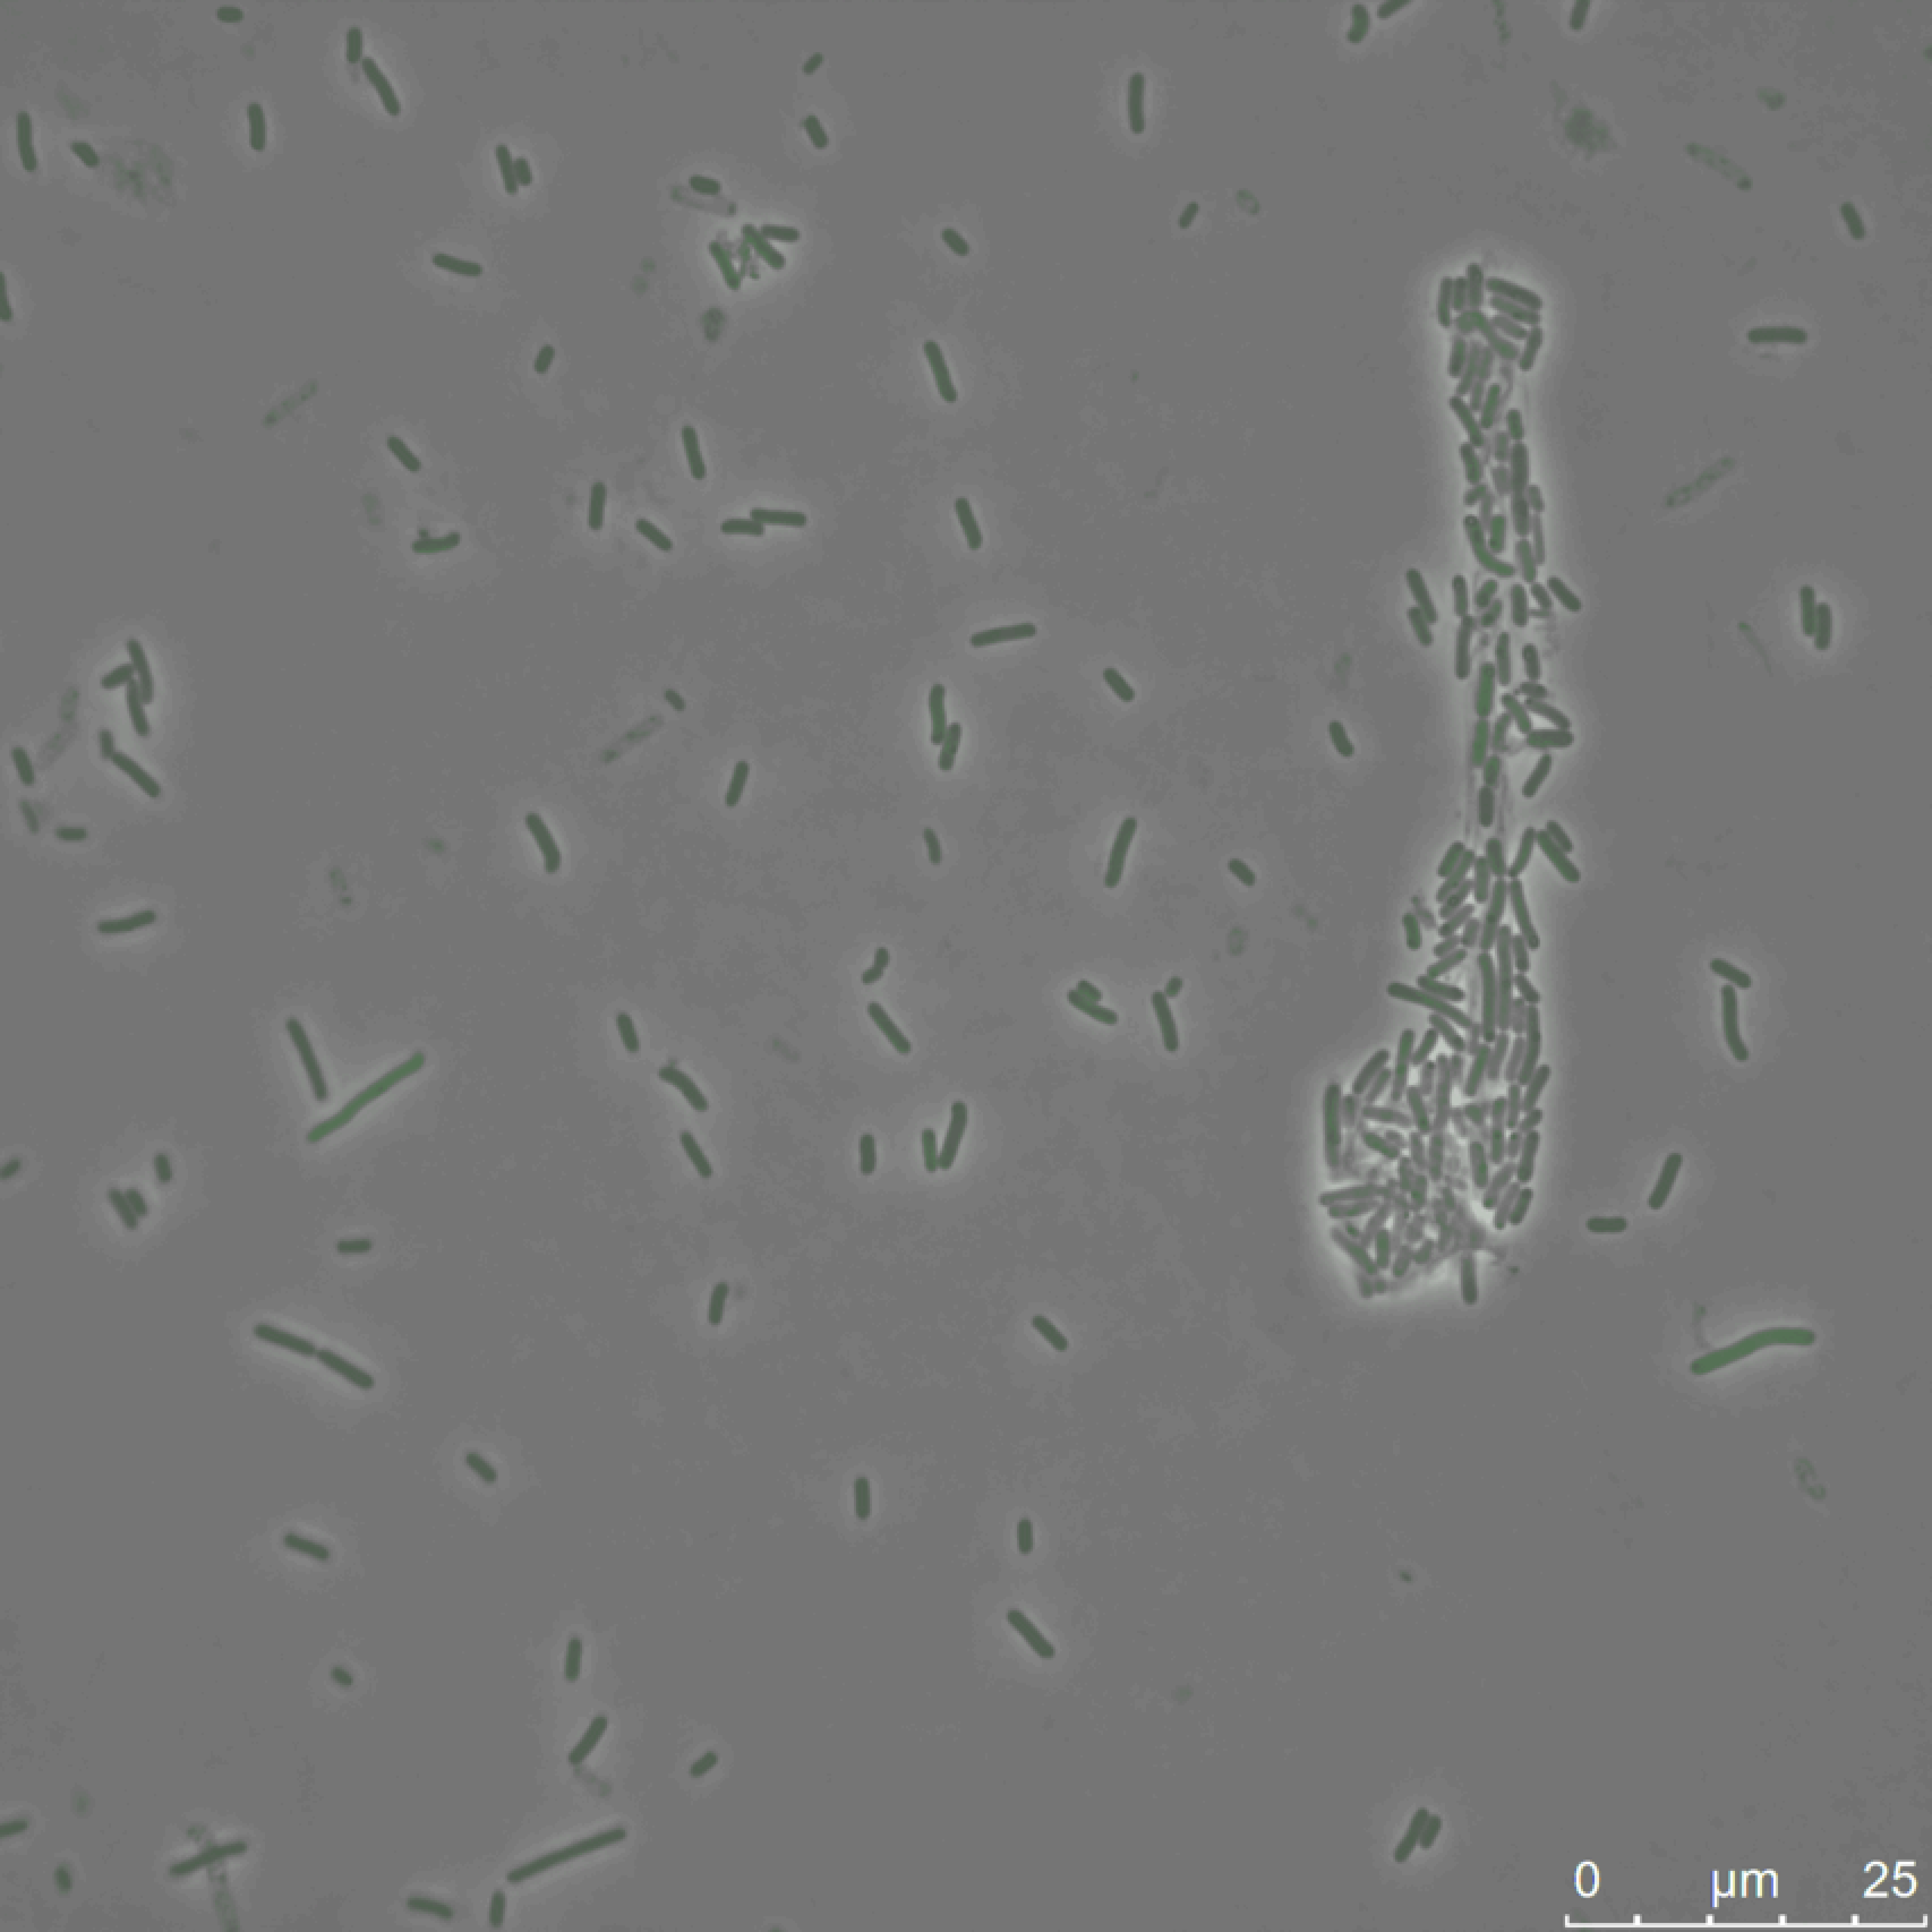
\includegraphics{TT01U1_24HR_2_LOWGREEN-crunch-lighter-resample.pdf} &%
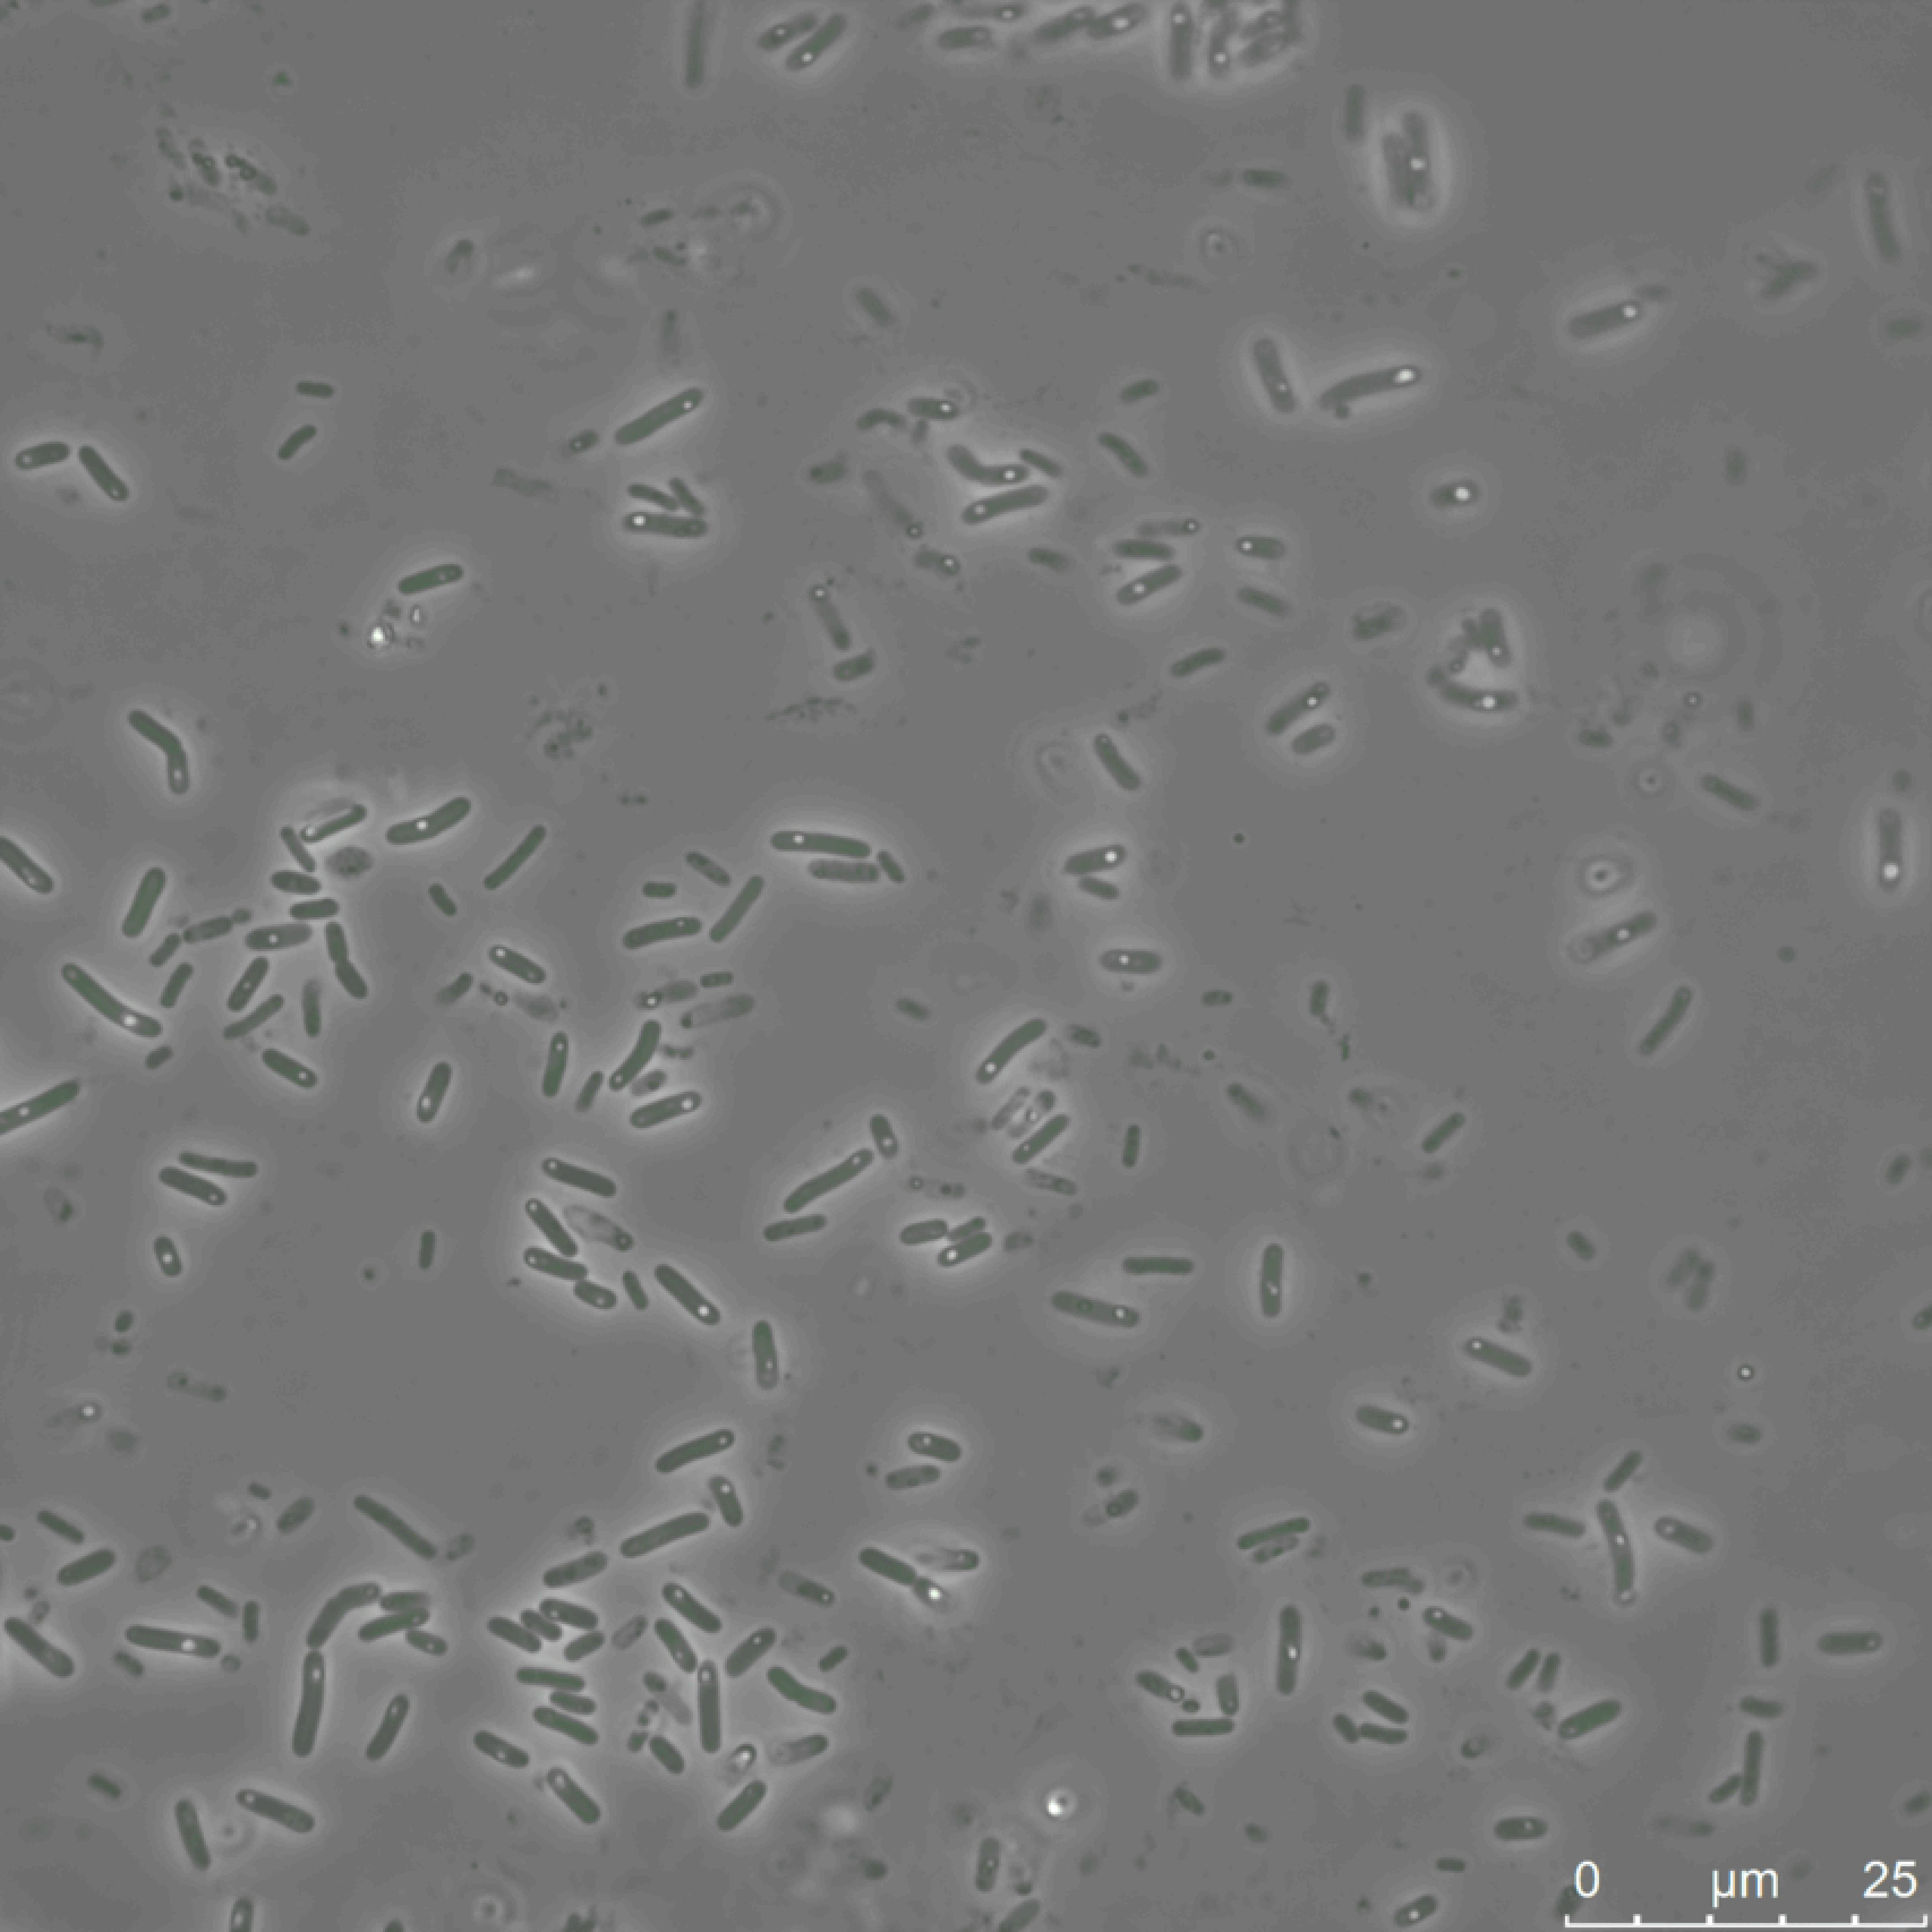
\includegraphics{TT01U1_72HR_2_LOWGREEN-crunch-lighter-resample.pdf} \\[-0.5ex]

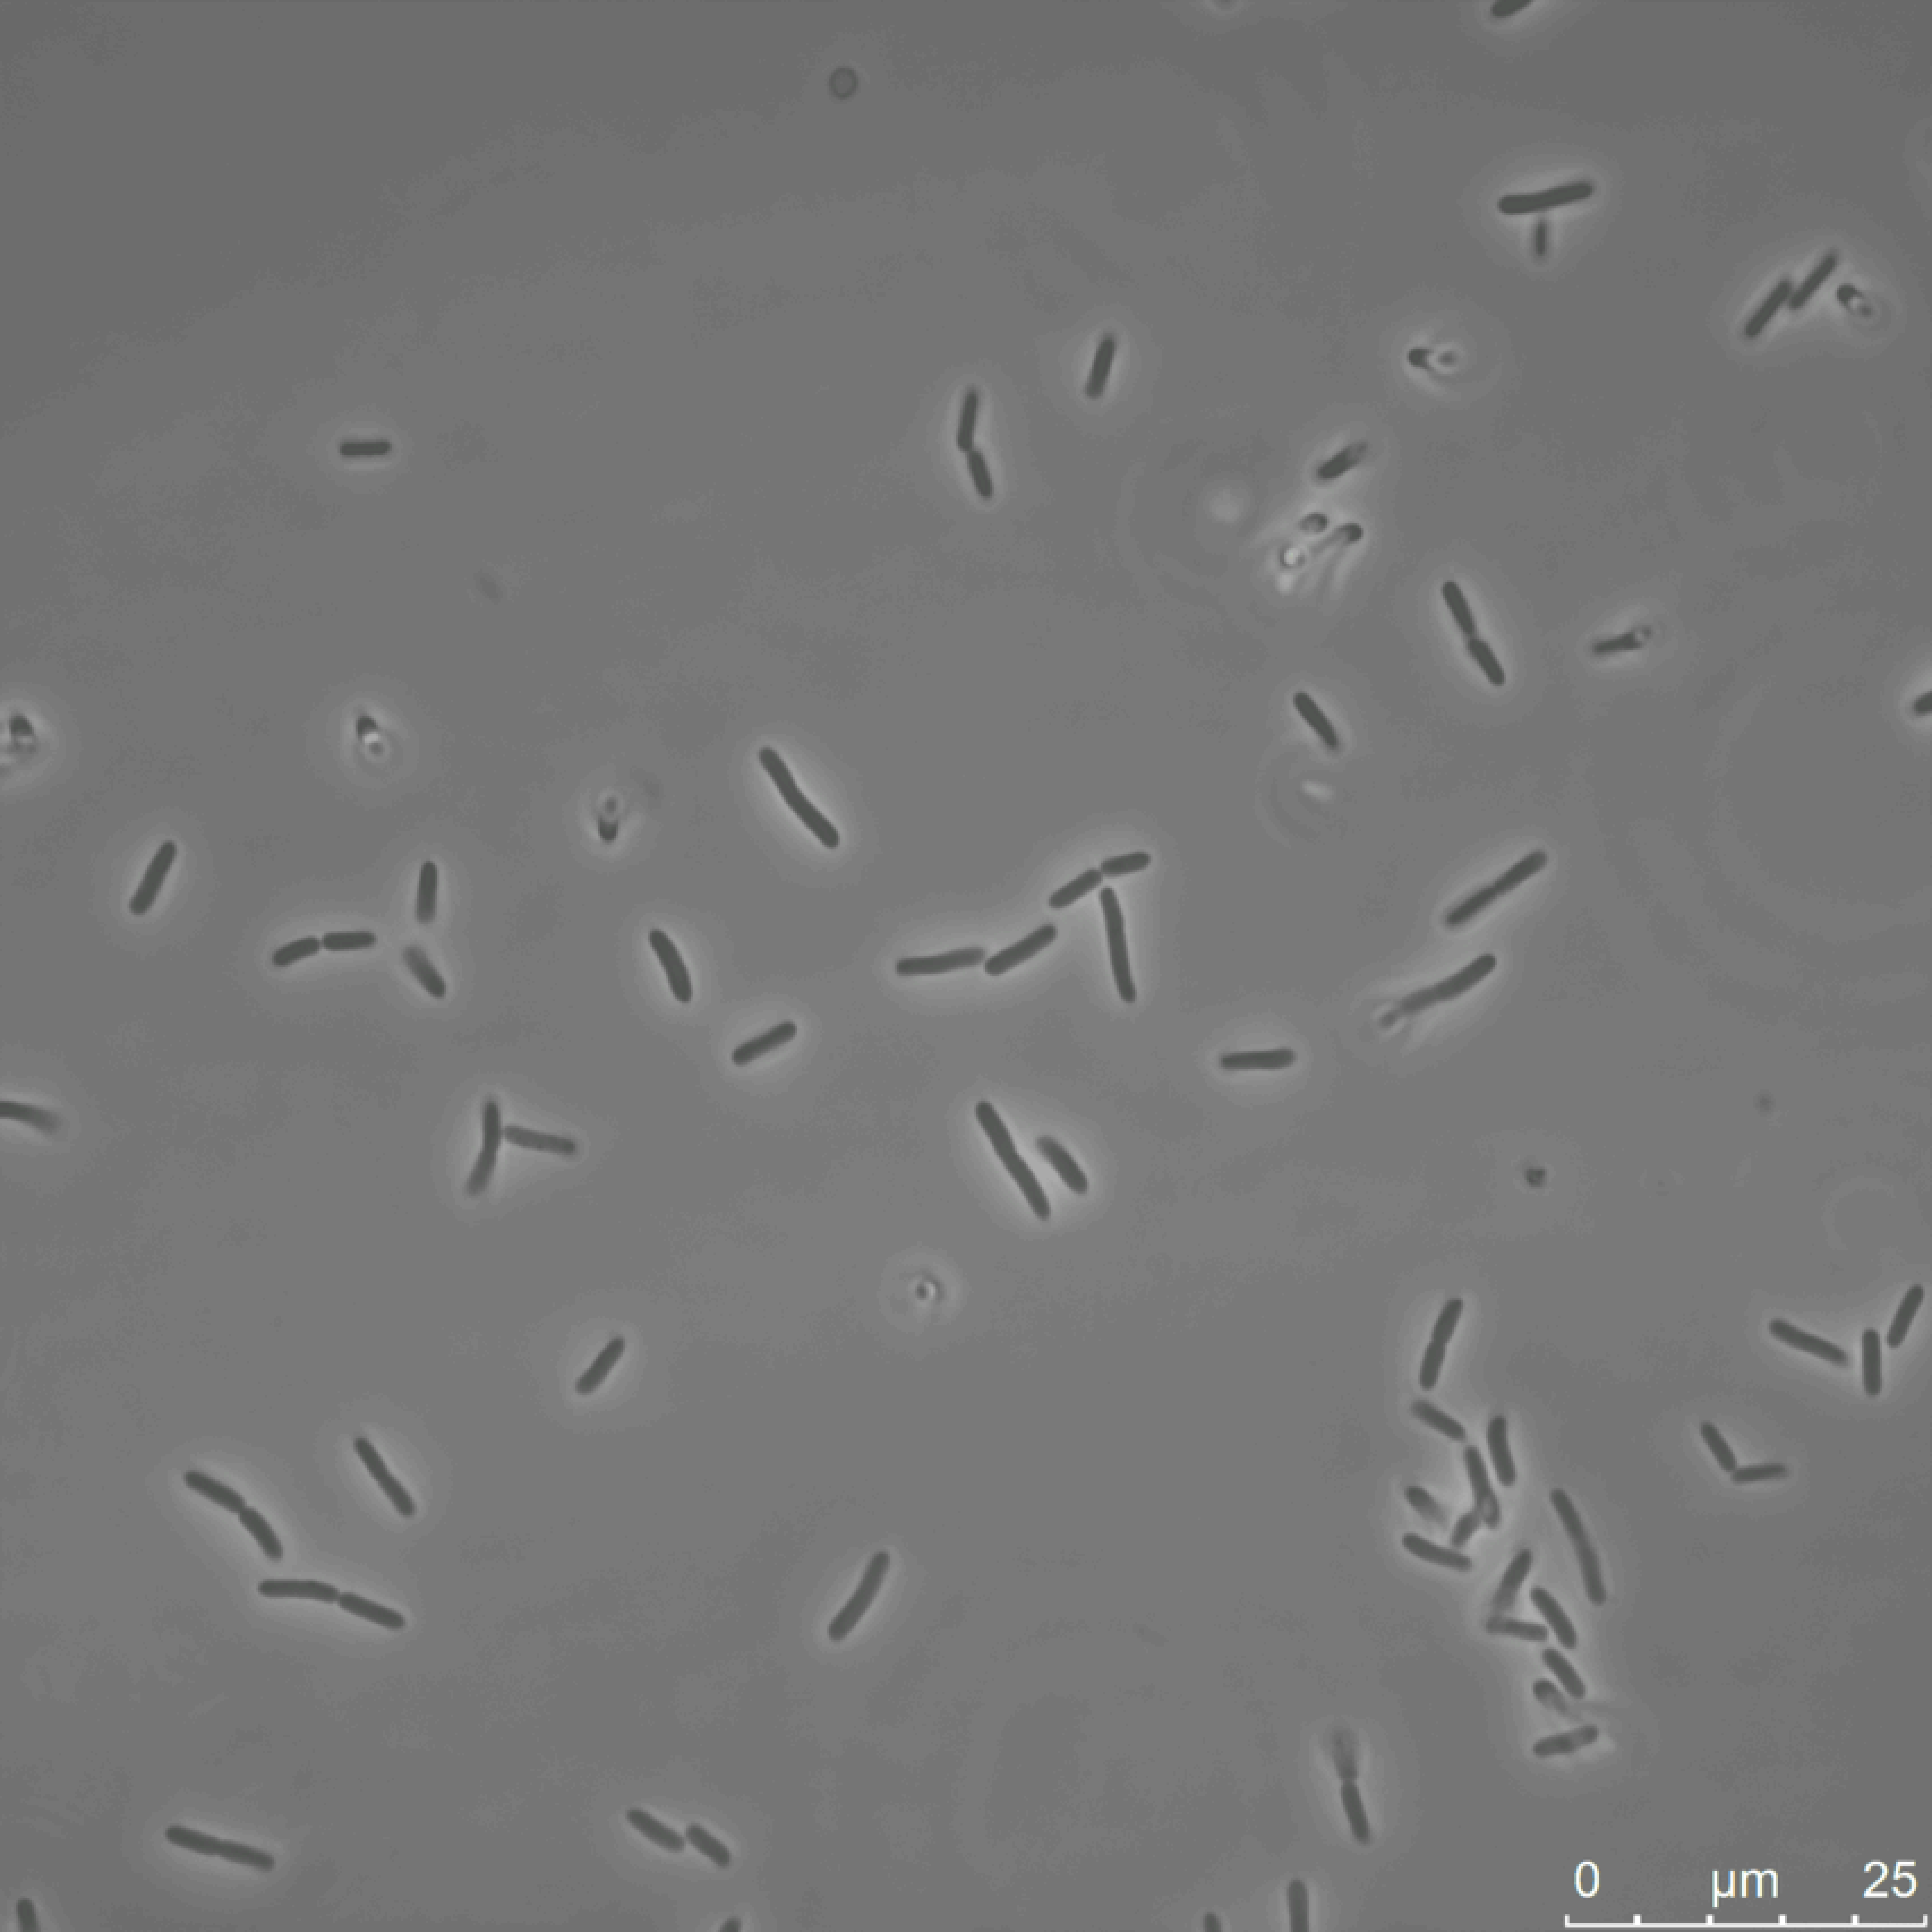
\includegraphics{TT01U1_3_NOGREEN-crunch-lighter-resample.pdf} &%
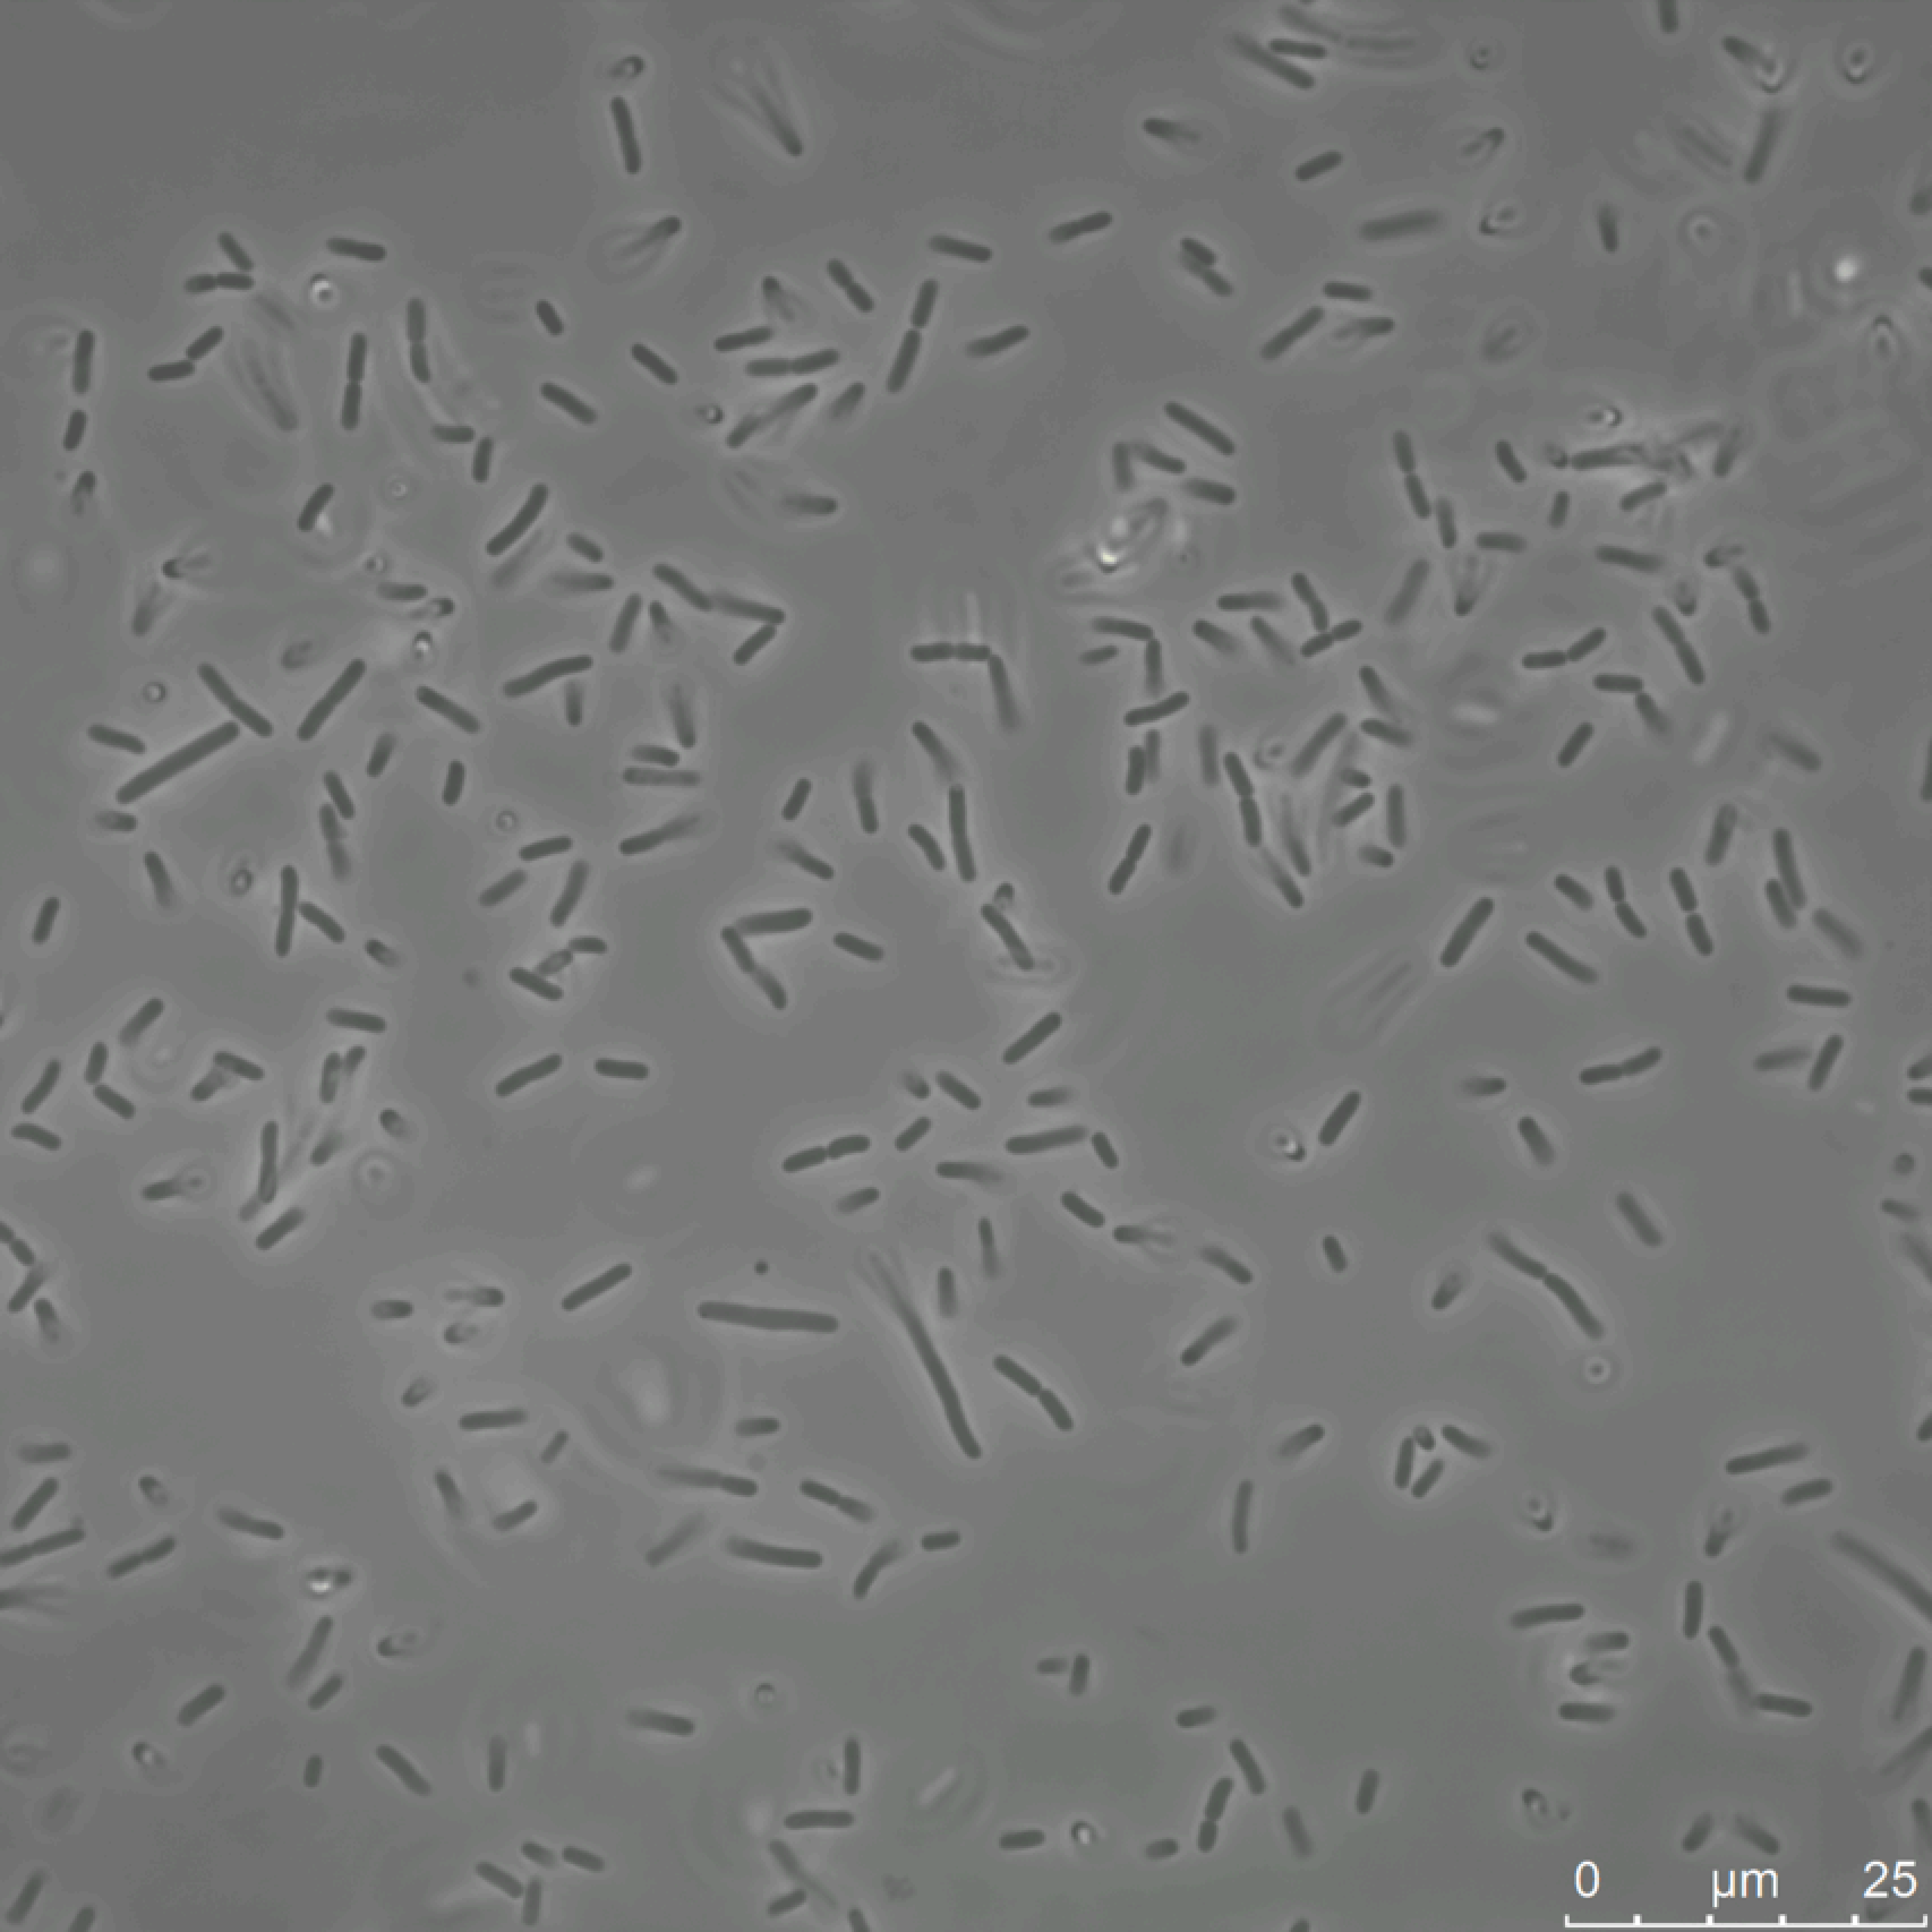
\includegraphics{TT01U1_5HR_3_LOWGREEN-crunch-lighter-resample.pdf} &%
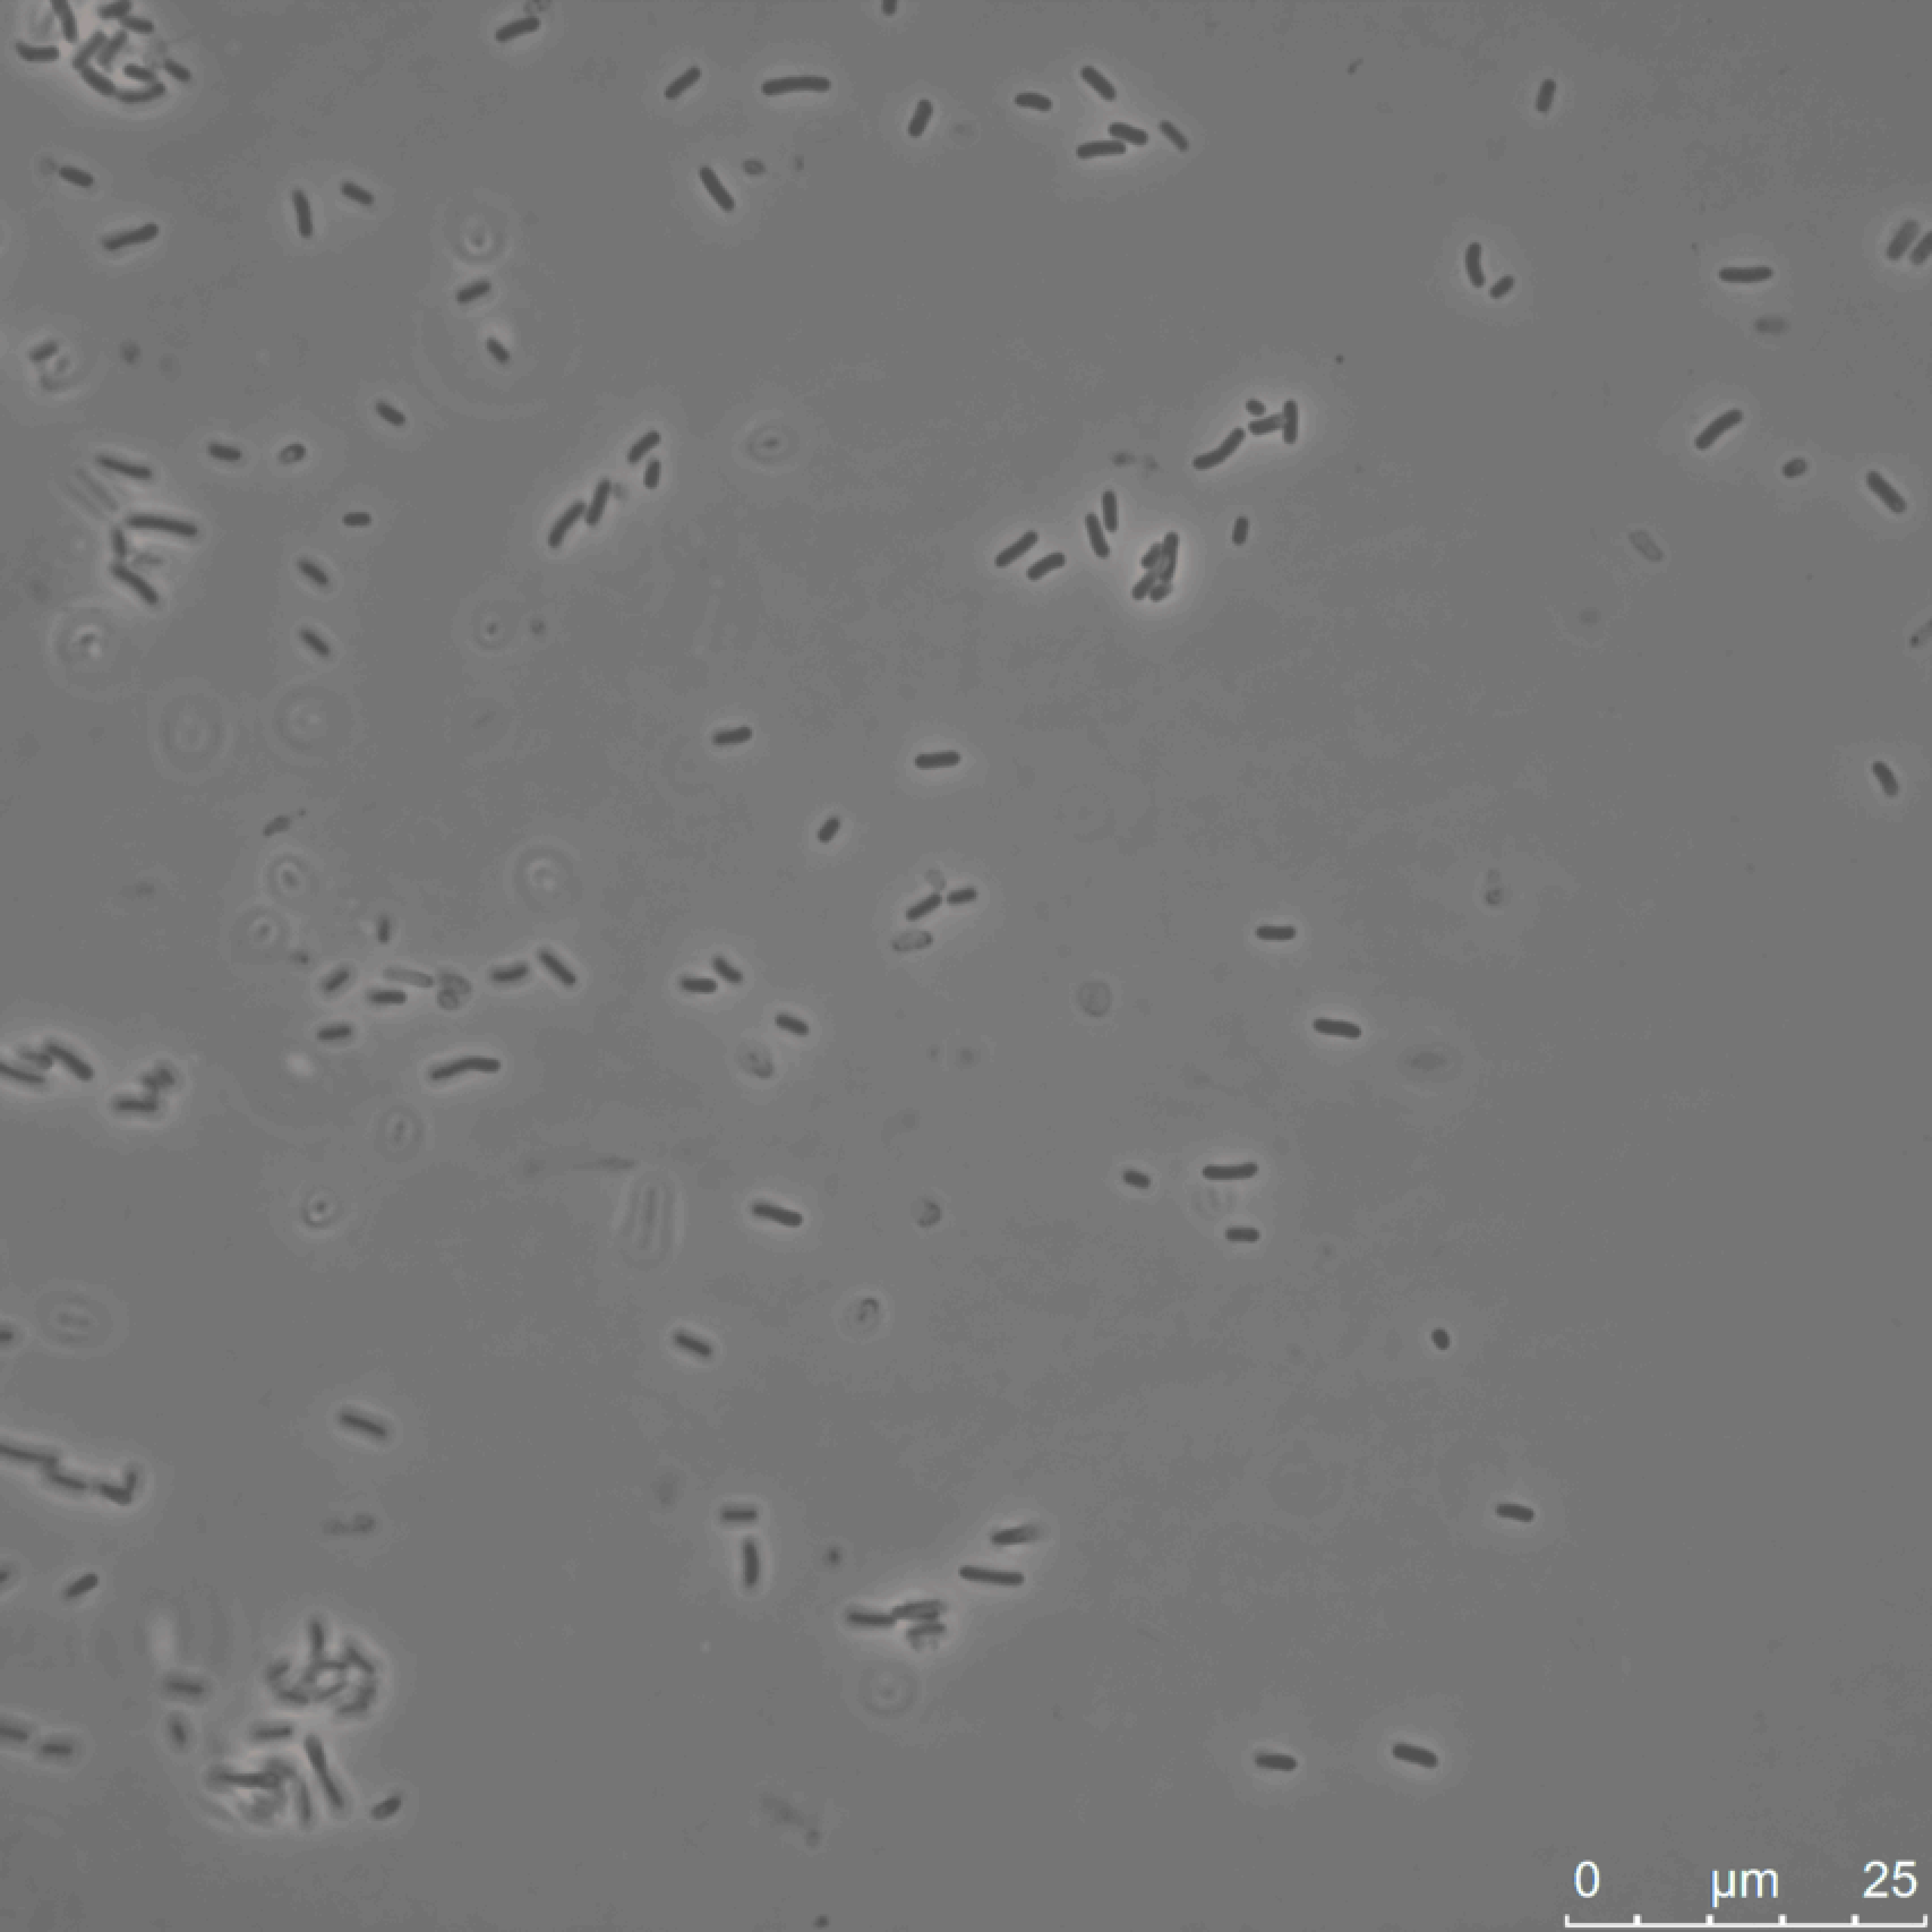
\includegraphics{TT01U1_24HR_3_GREEN-crunch-lighter-resample.pdf} &%
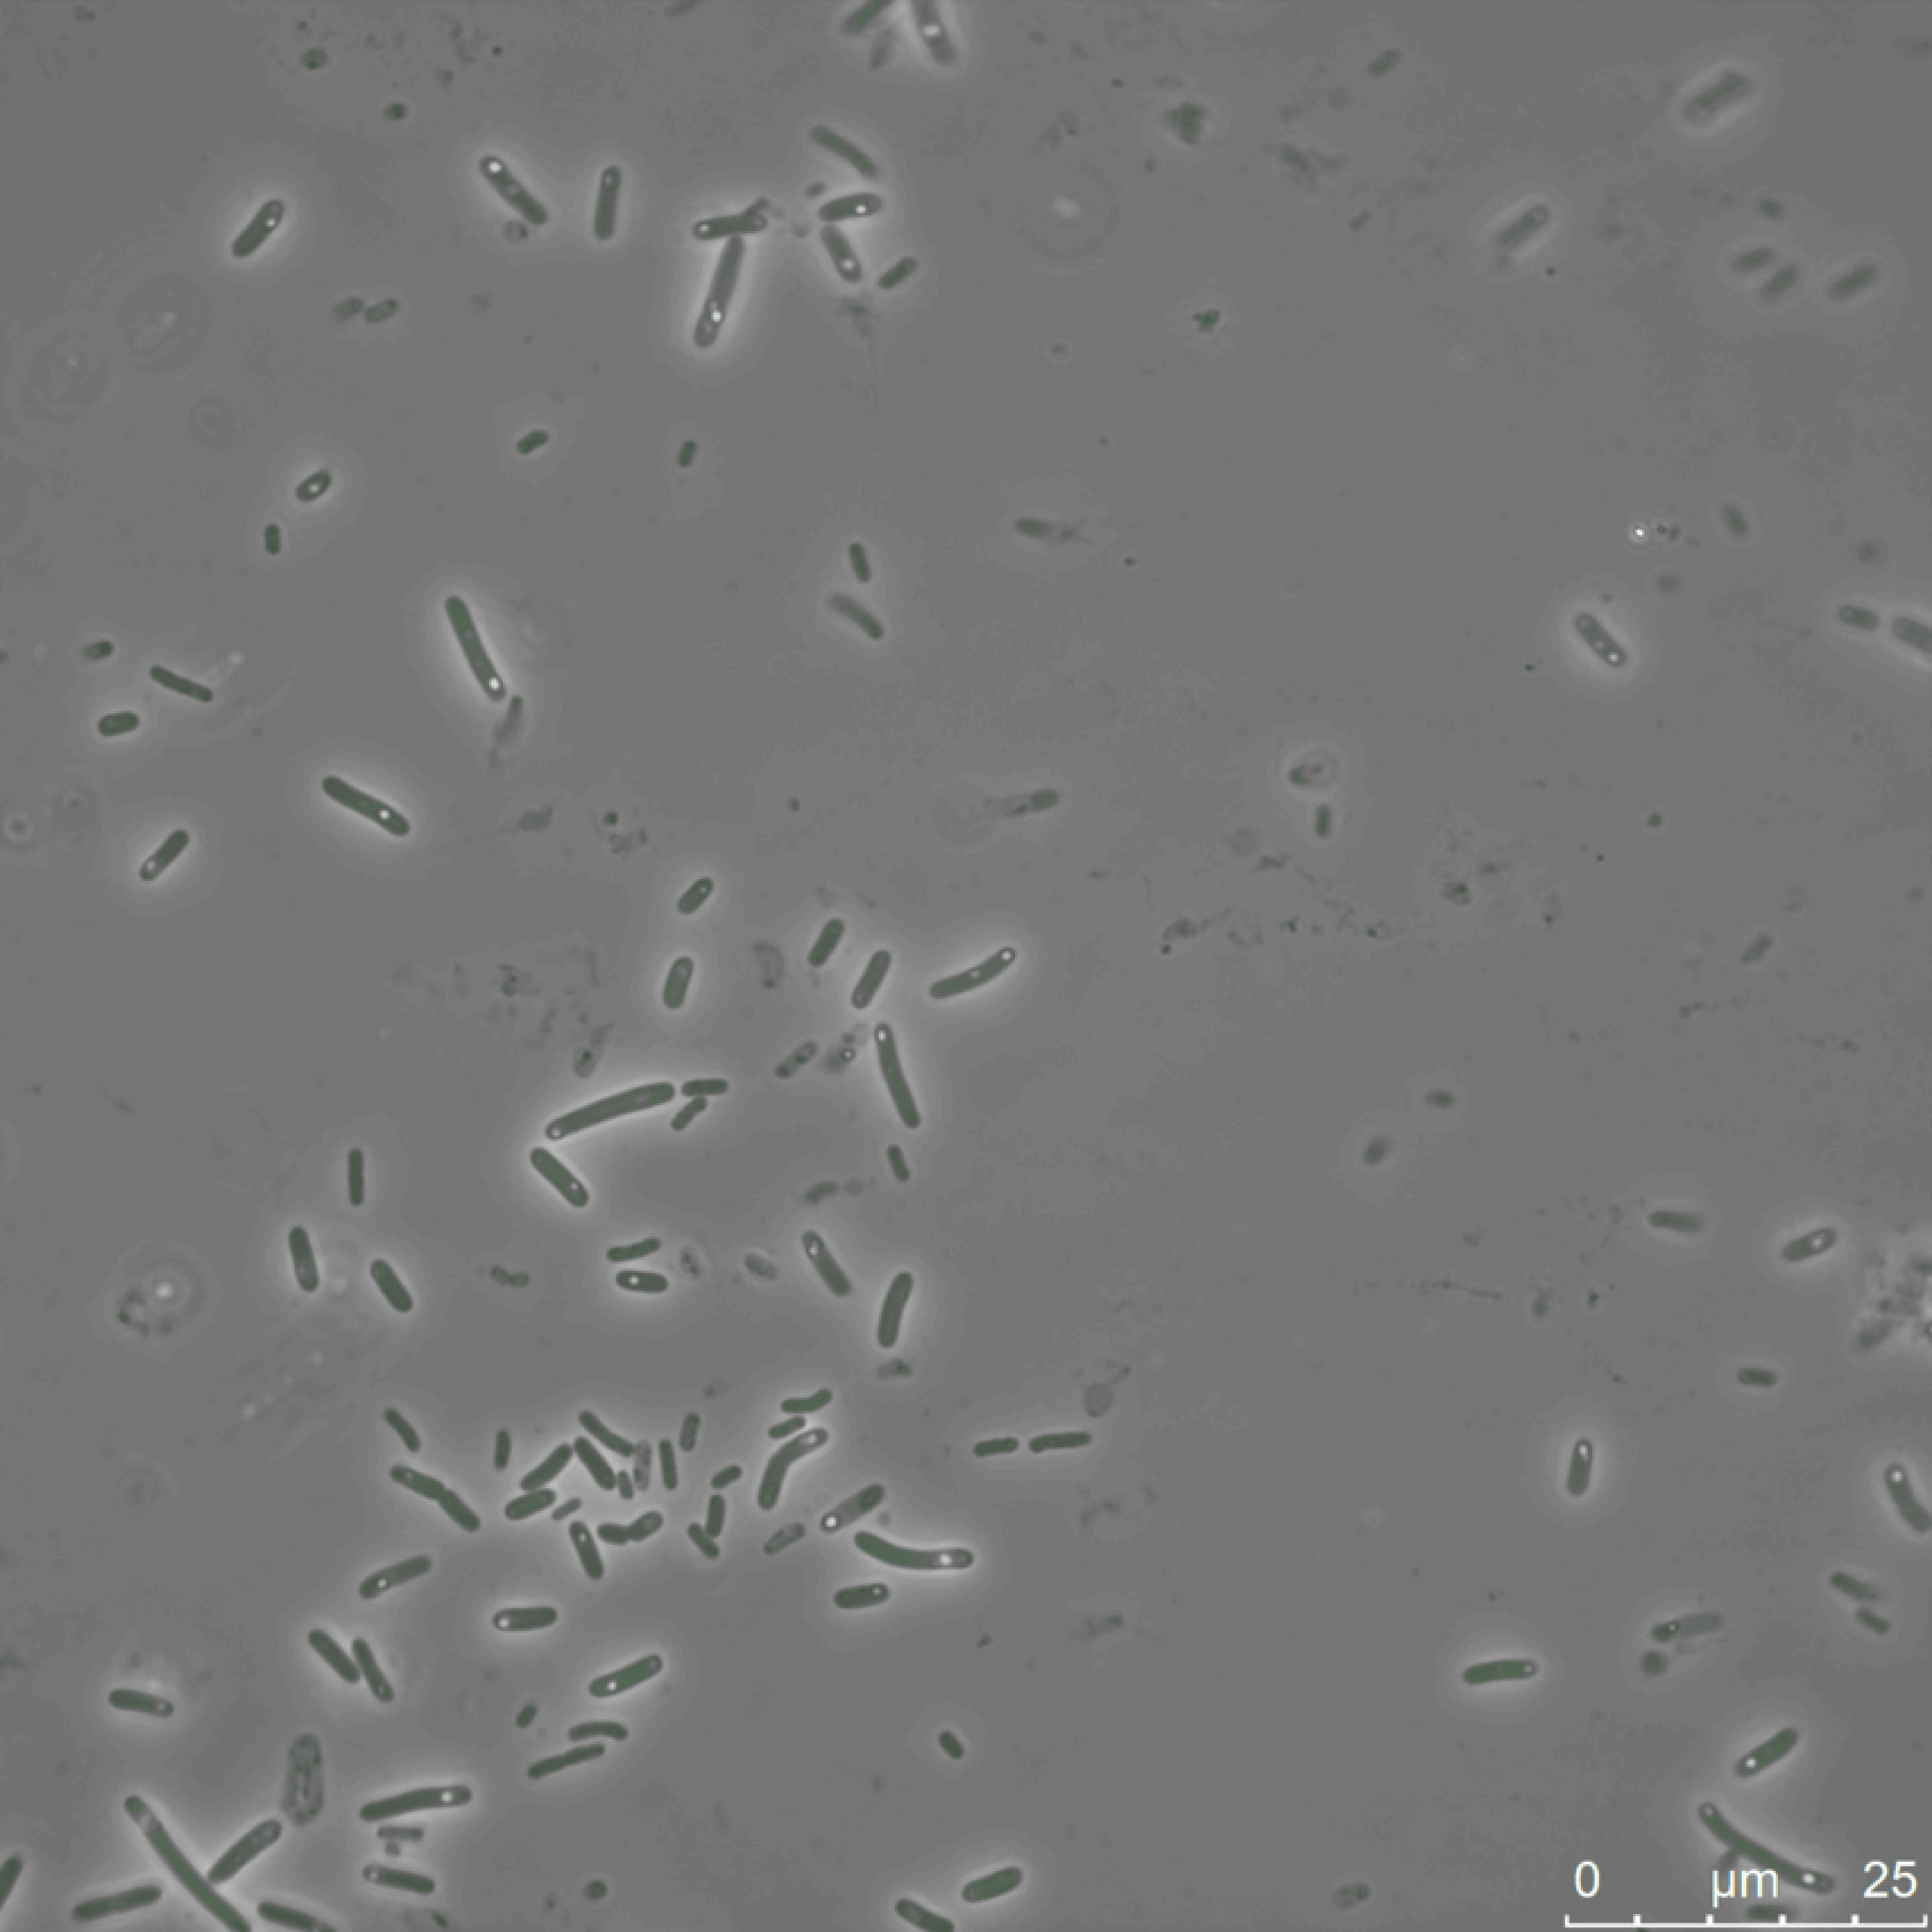
\includegraphics{TT01U1_72HR_3_LOWGREEN-crunch-lighter-resample.pdf} \\[-0.5ex]

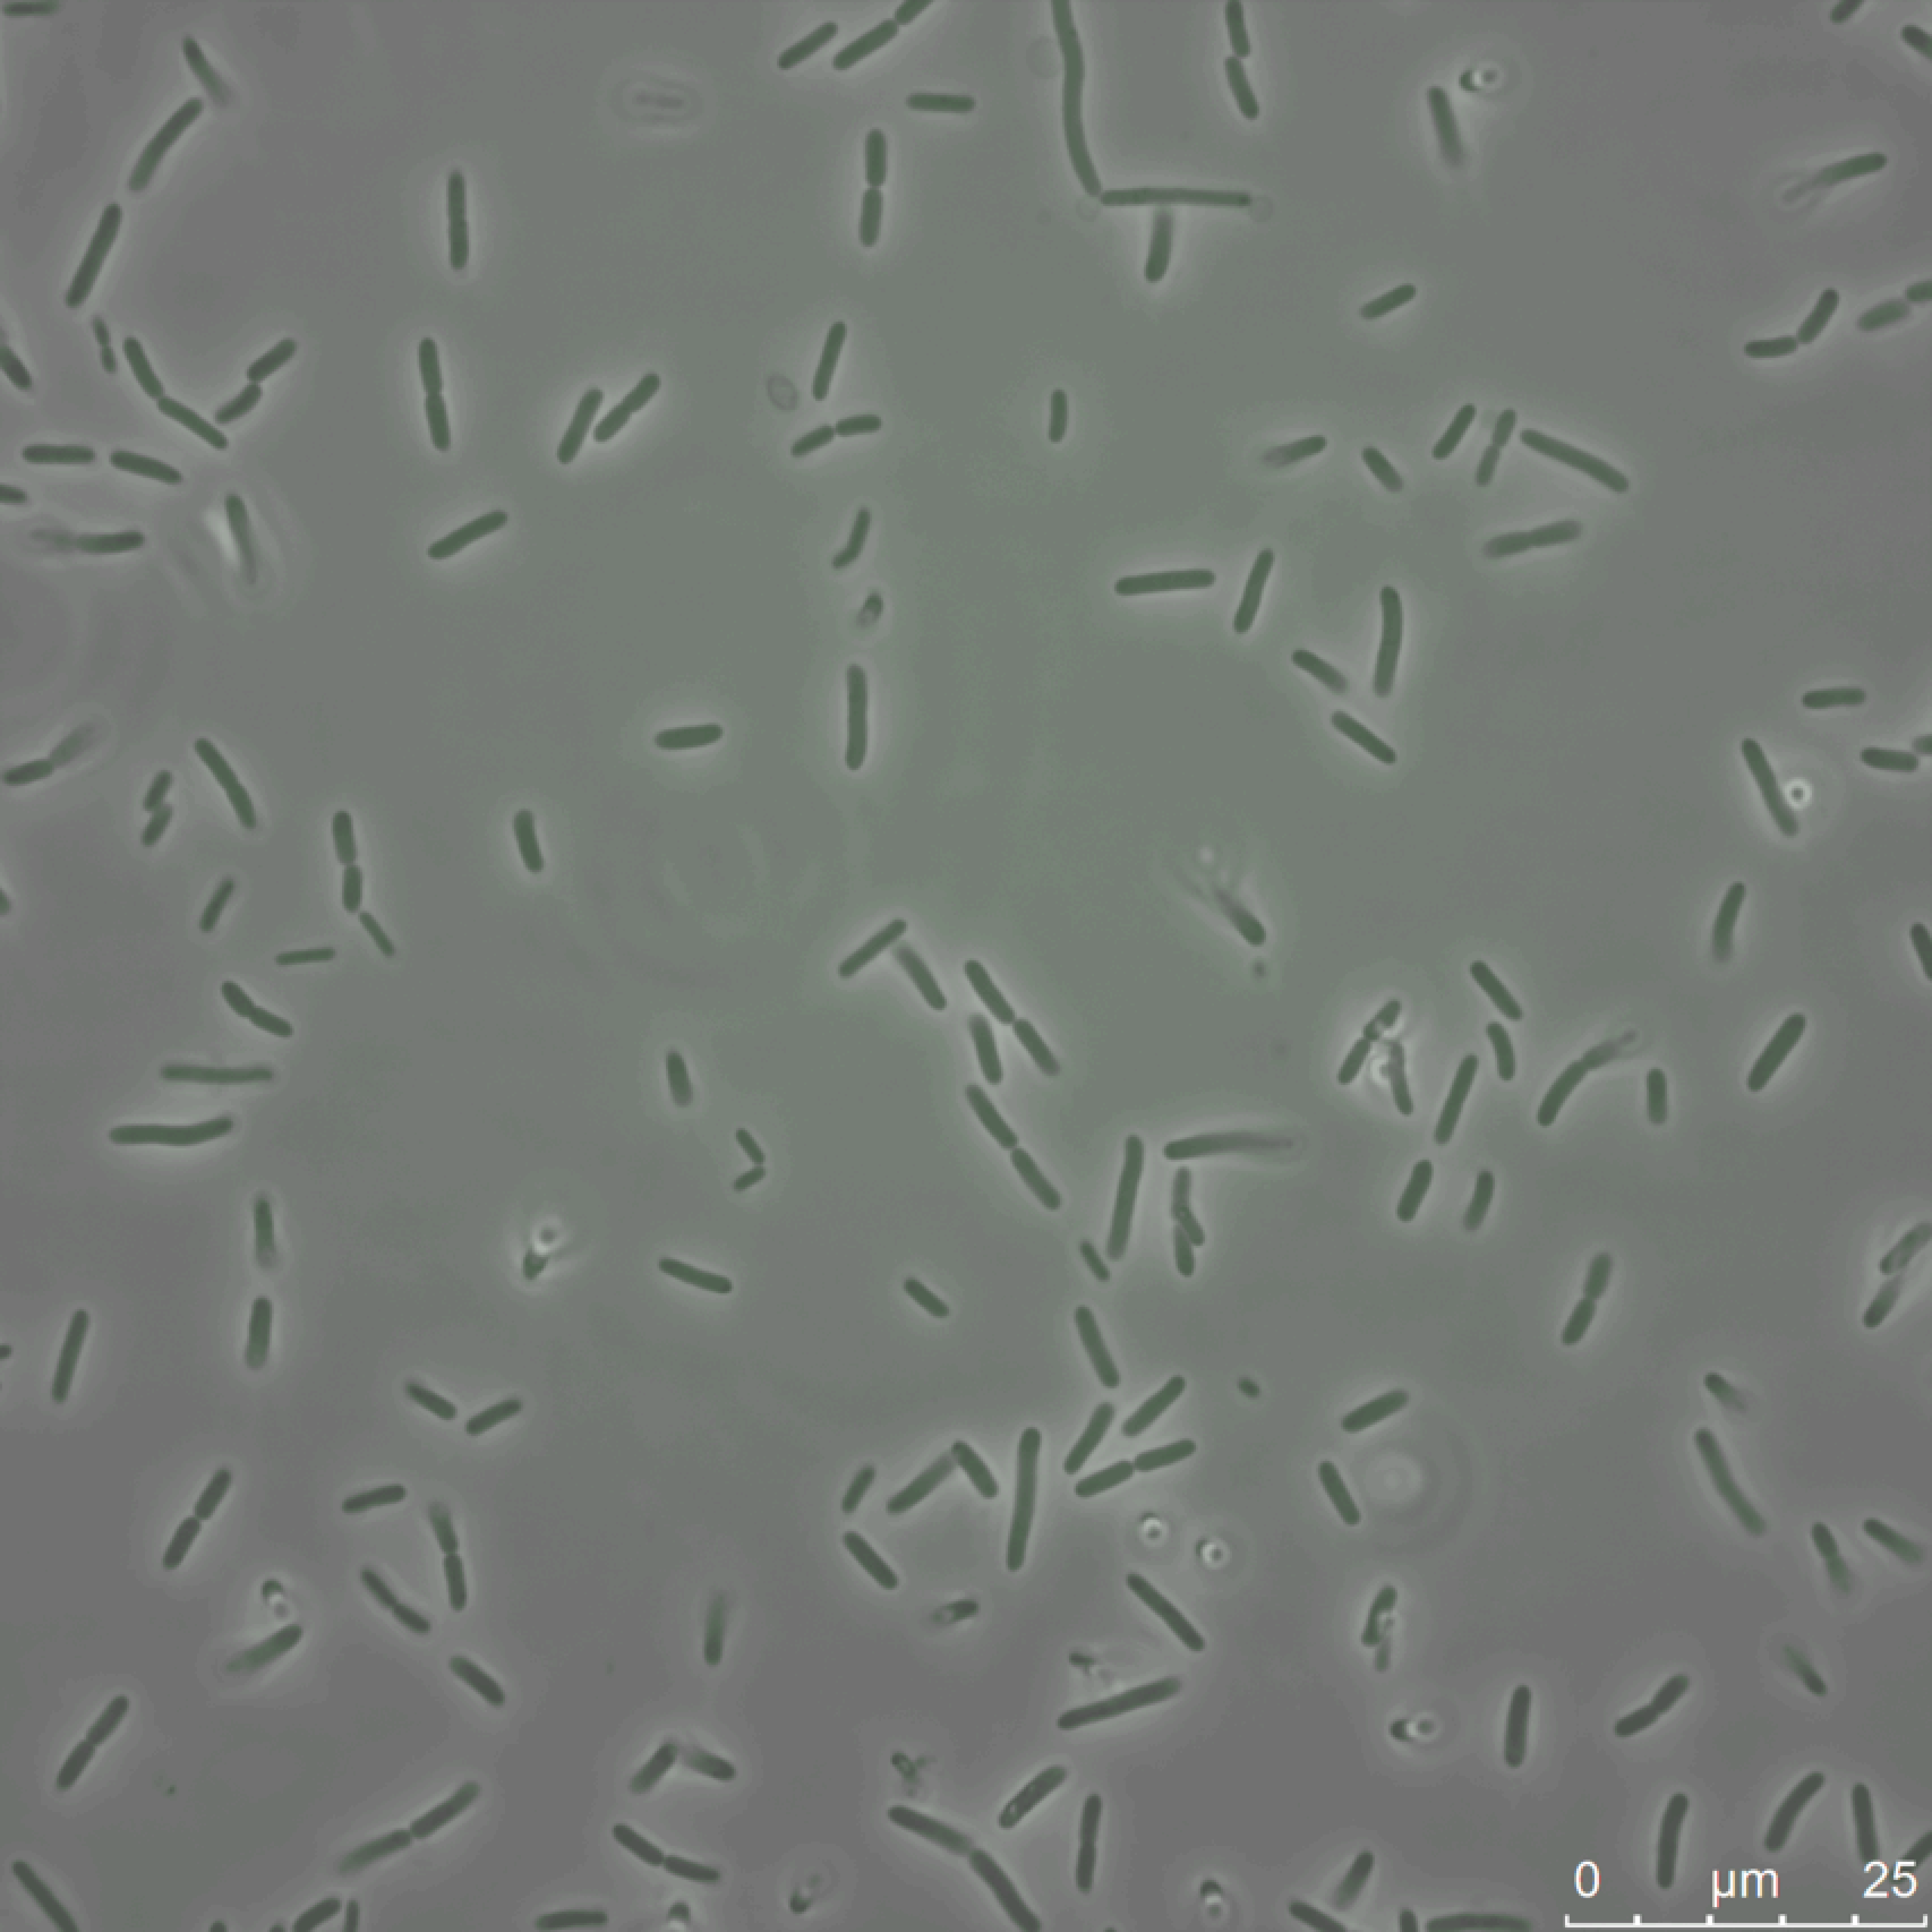
\includegraphics{TT01U1_4_NOGREEN-crunch-lighter-resample.pdf} &%
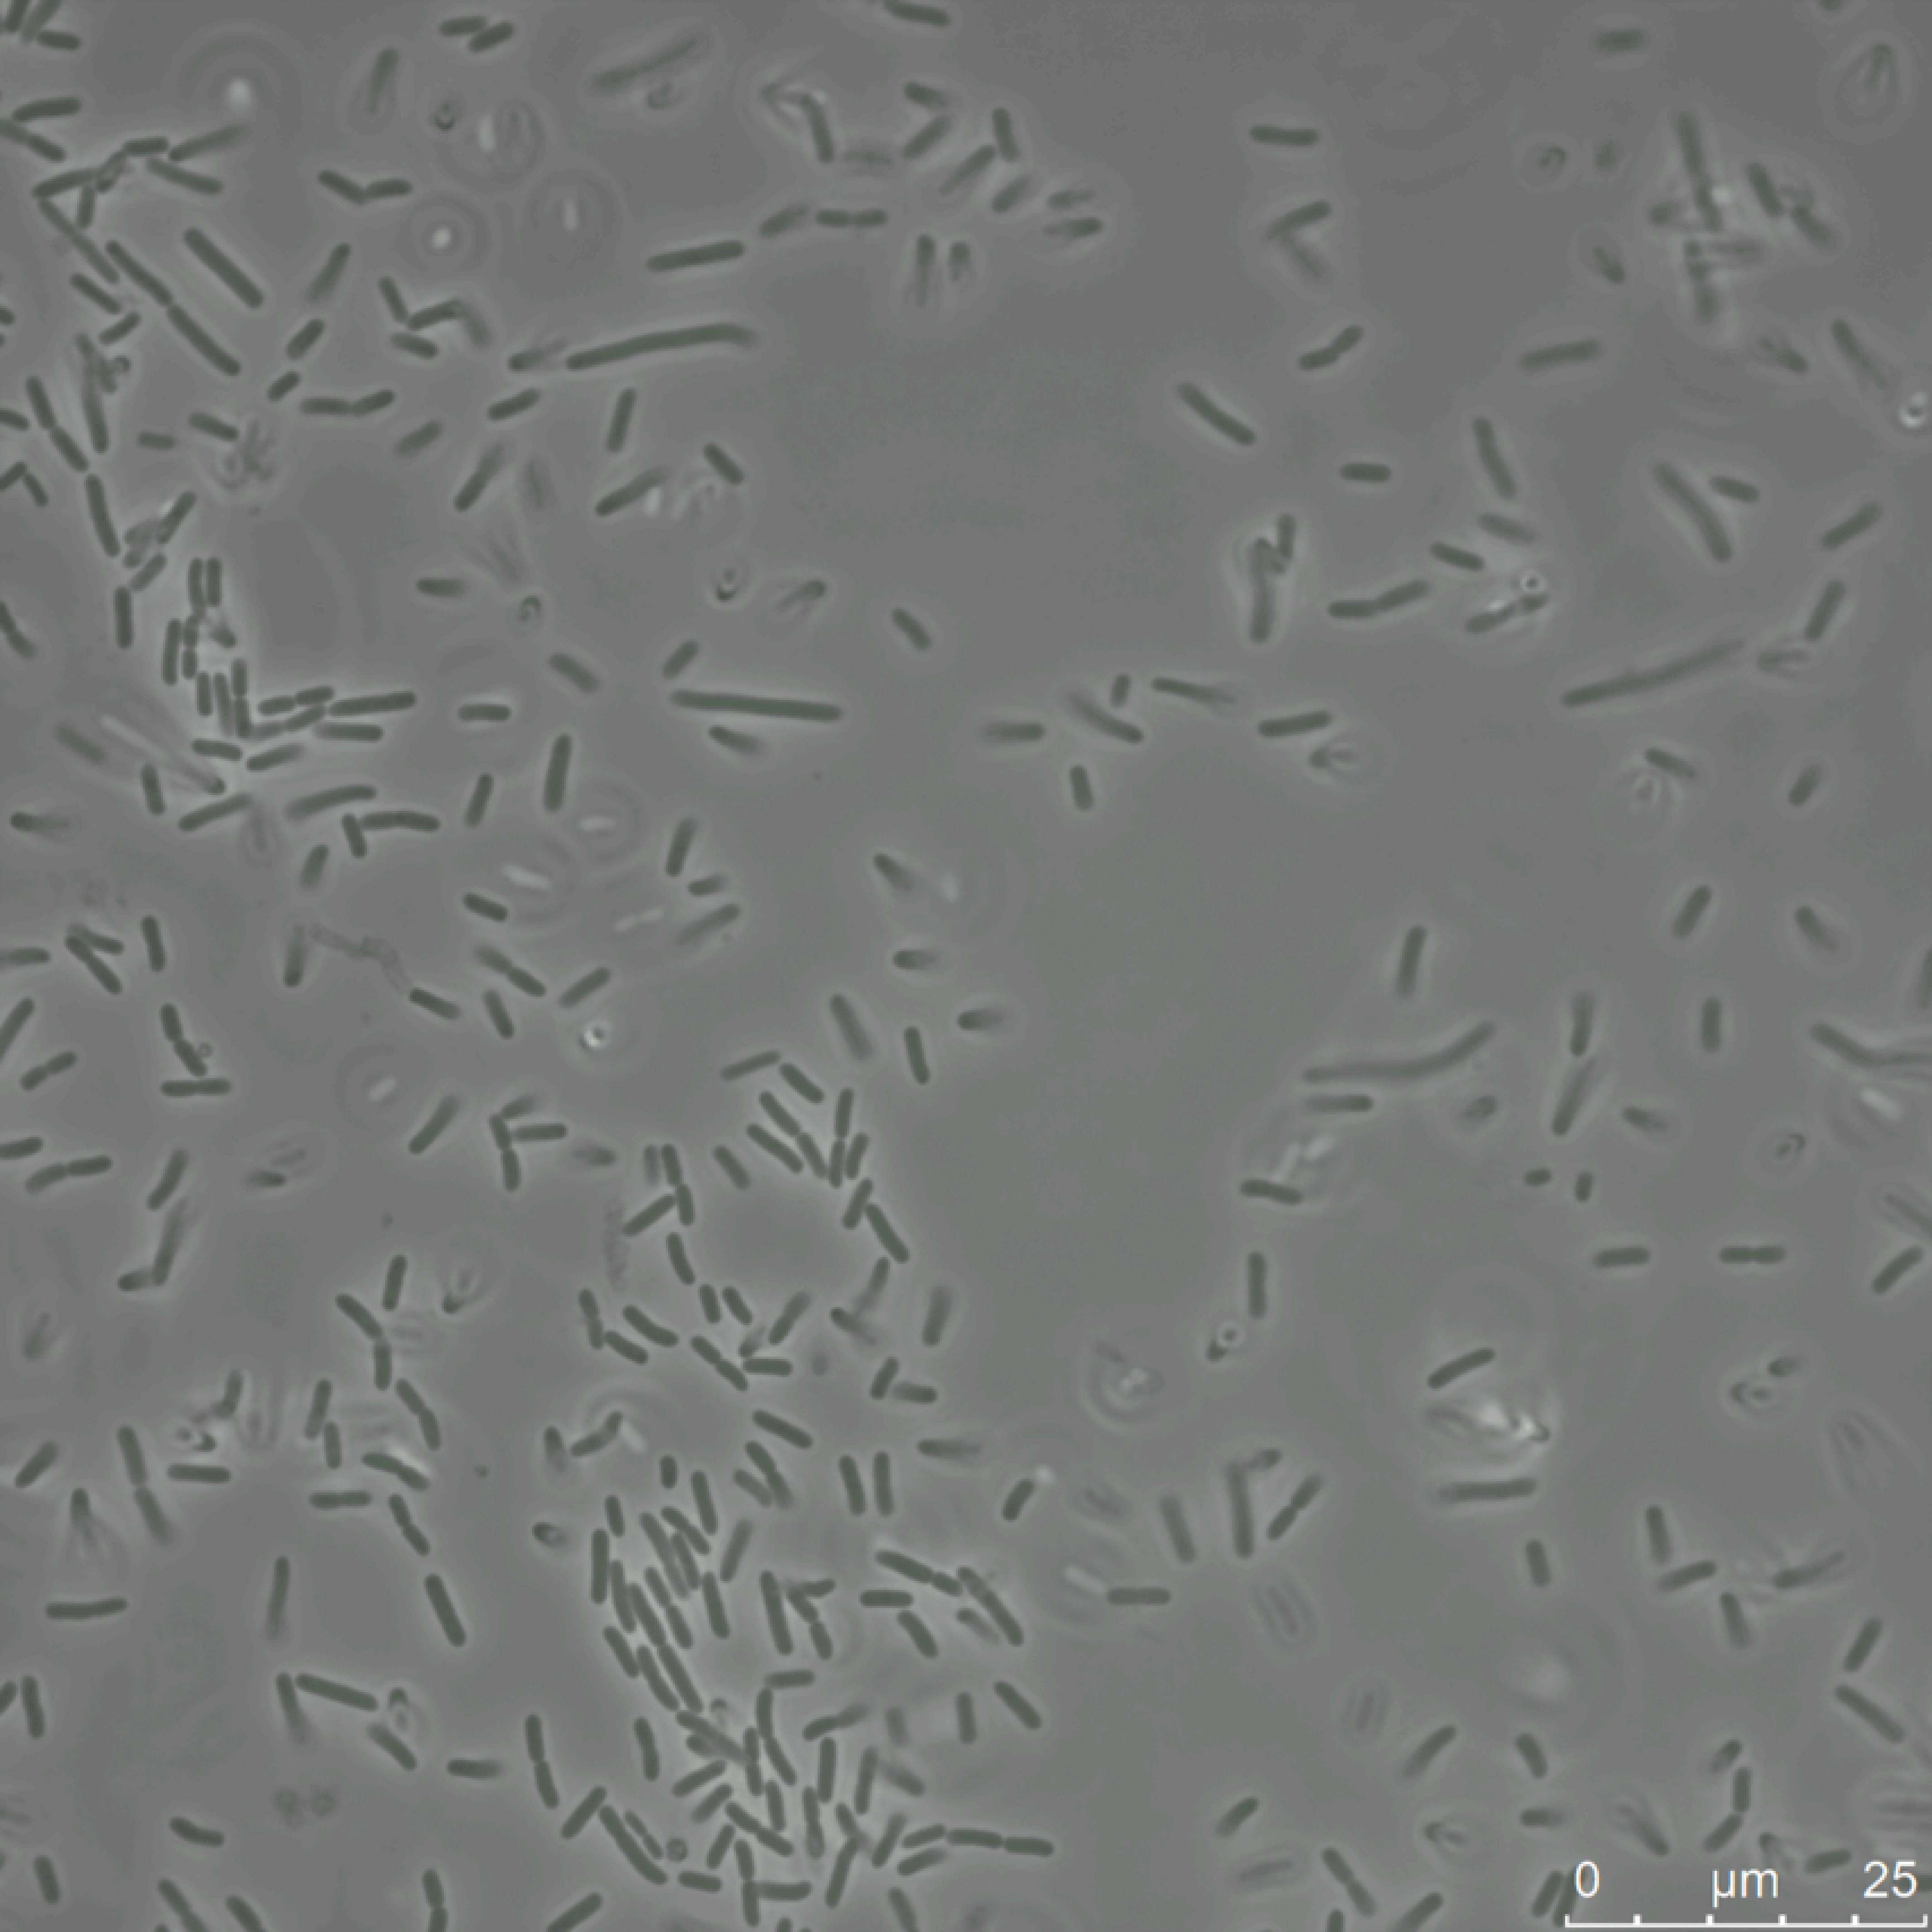
\includegraphics{TT01U1_5HR_4_LOWGREEN-crunch-lighter-resample.pdf} &%
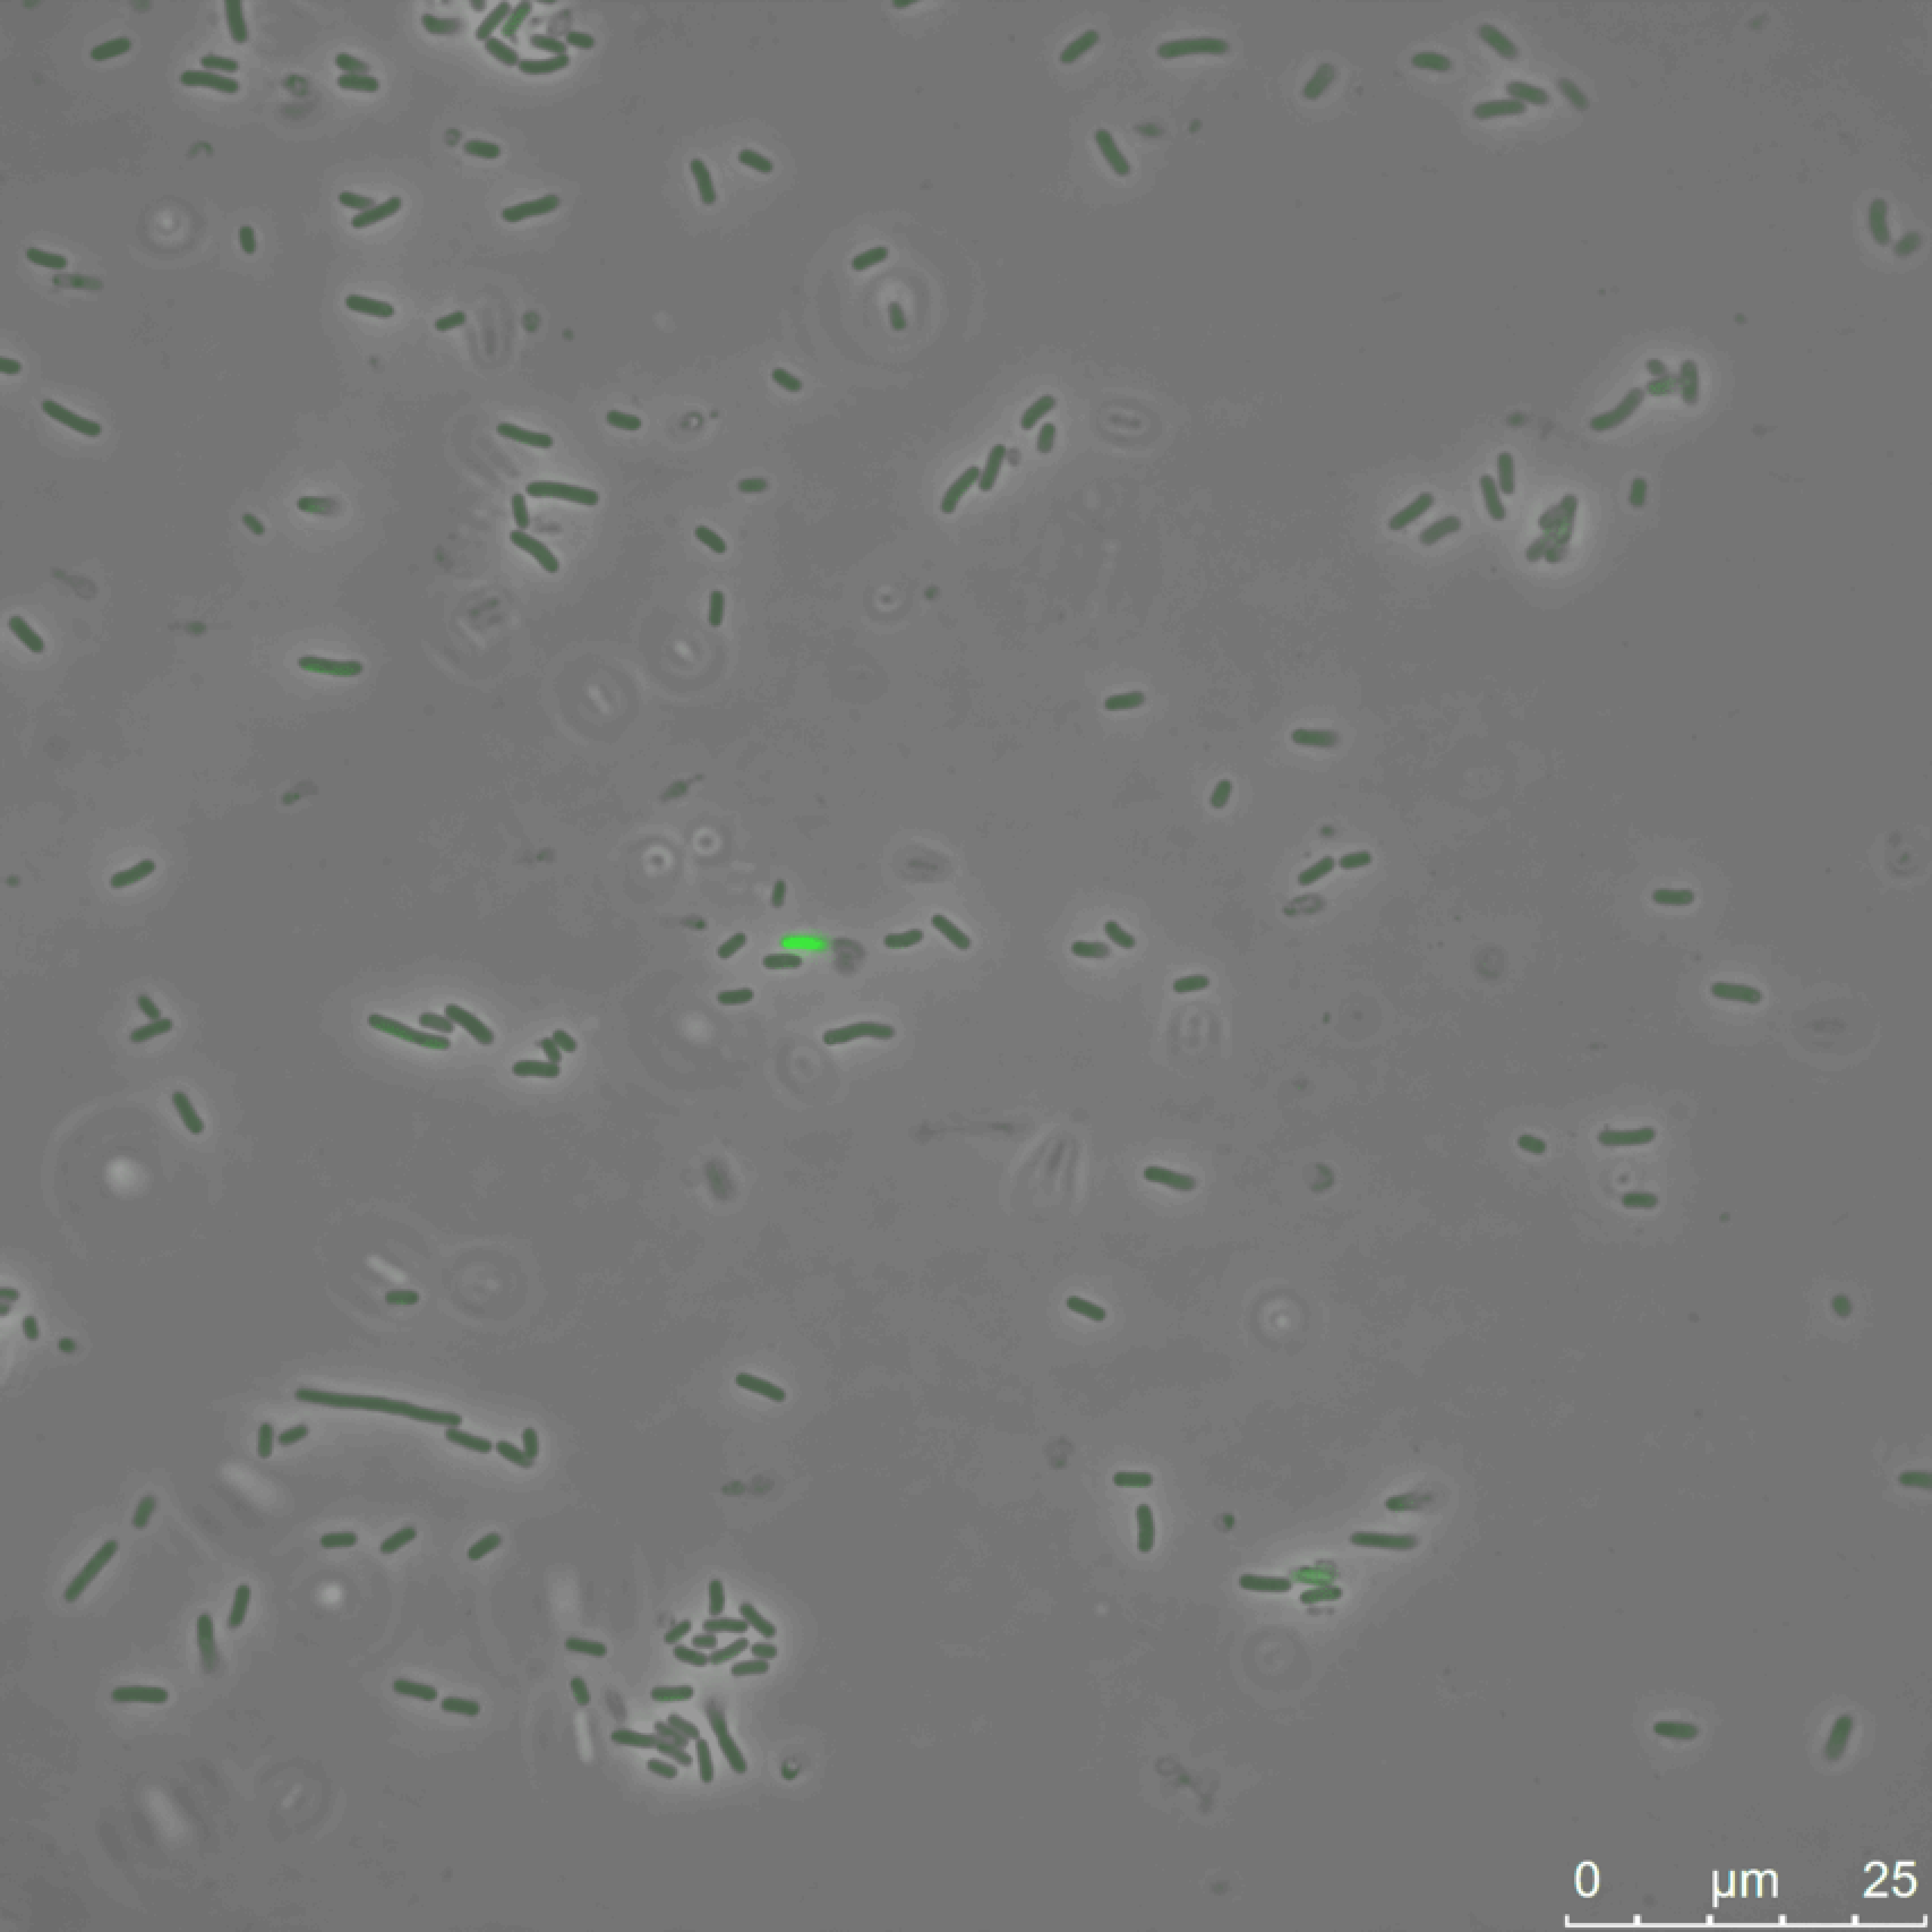
\includegraphics{TT01U1_24HR_4_GREEN-crunch-lighter-resample.pdf} &%
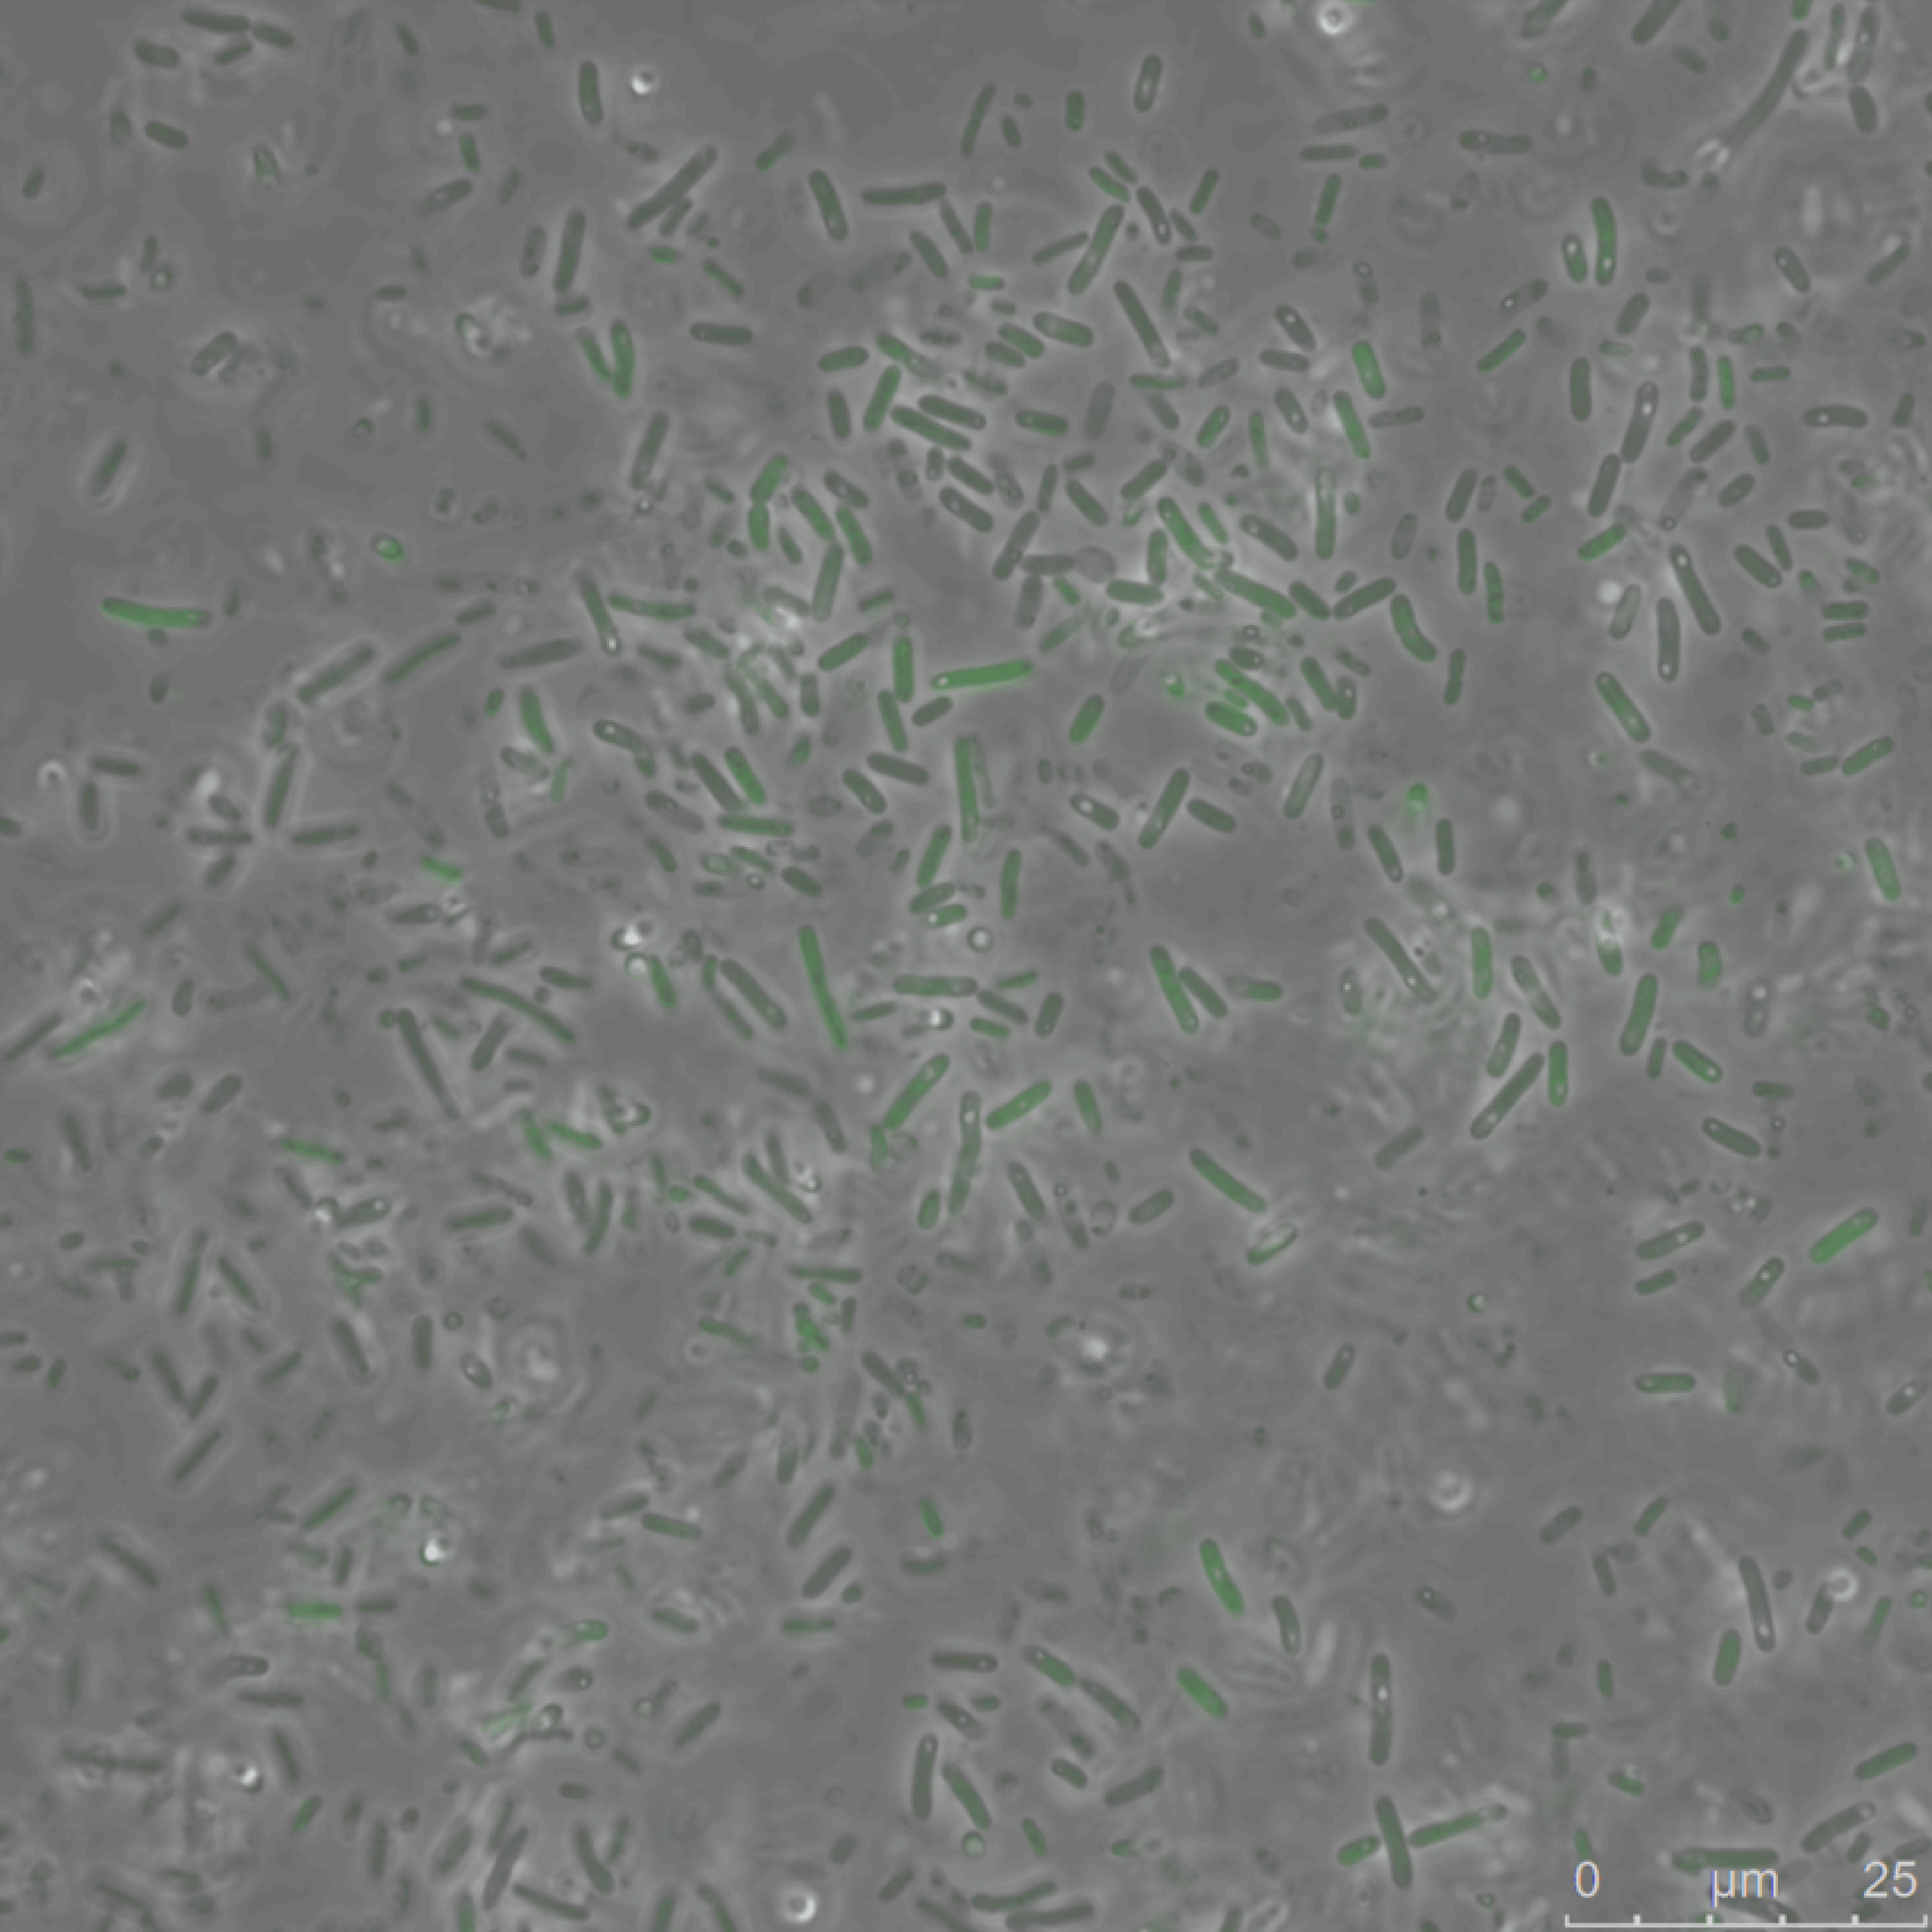
\includegraphics{TT01U1_72HR_5_GREEN-crunch-lighter-resample.pdf} \\
 - & - &  ++ & ++ \\[1ex]

\end{tabularx}

\captionsetup{singlelinecheck=off, justification=justified, font=footnotesize, aboveskip=20pt}
\caption[Reporter microscopy - TT01 Unit 1]{\textsc{\normalsize Reporter microscopy for the \emph{P. luminescens} TT01 ``Unit 1" promoter.}\vspace{0.1cm} \newline A representative selection of images for 4 time points, for the PVC ``Unit 1" promoter fusion. Quadruplicate images are displayed vertically as representative of the whole slide sample. Key to qualitative fluorescence indication: ``-" - no fluorescence, ``+" - low level fluorescence in isolated cells. ``++" - low level fluorescence in many cells or few brighter cells, ``+++" - intermediate to high fluorescence in almost all cells, or very bright isolated cells.}
\end{figure}\label{RMTT01U1}
\endgroup

%%%%%%%%%%%%%%%%%%%%%%%%%%%%%%%%%%%%%%%%%%%%%%%%%%%%%%%%%%%%%%%%%%%%

\begingroup
\renewcommand{\arraystretch}{0.8}%
\setlength{\tabcolsep}{0.3pt}
\begin{figure}[p]
\setkeys{Gin}{width=\linewidth}
\Huge
\begin{tabularx}{\textwidth}{CCCC}
\multicolumn{4}{p{\linewidth}}{\large \centering \textbf{\emph{P. asymbiotica} PB68.1 (``THAI") PVC ``Unit 1"}} \\
\hiderowcolors
& & & \\[-1.5ex]
\Large 2 Hours &\Large 5 Hours &\Large 24 Hours &\Large 72 Hours \\[1ex]

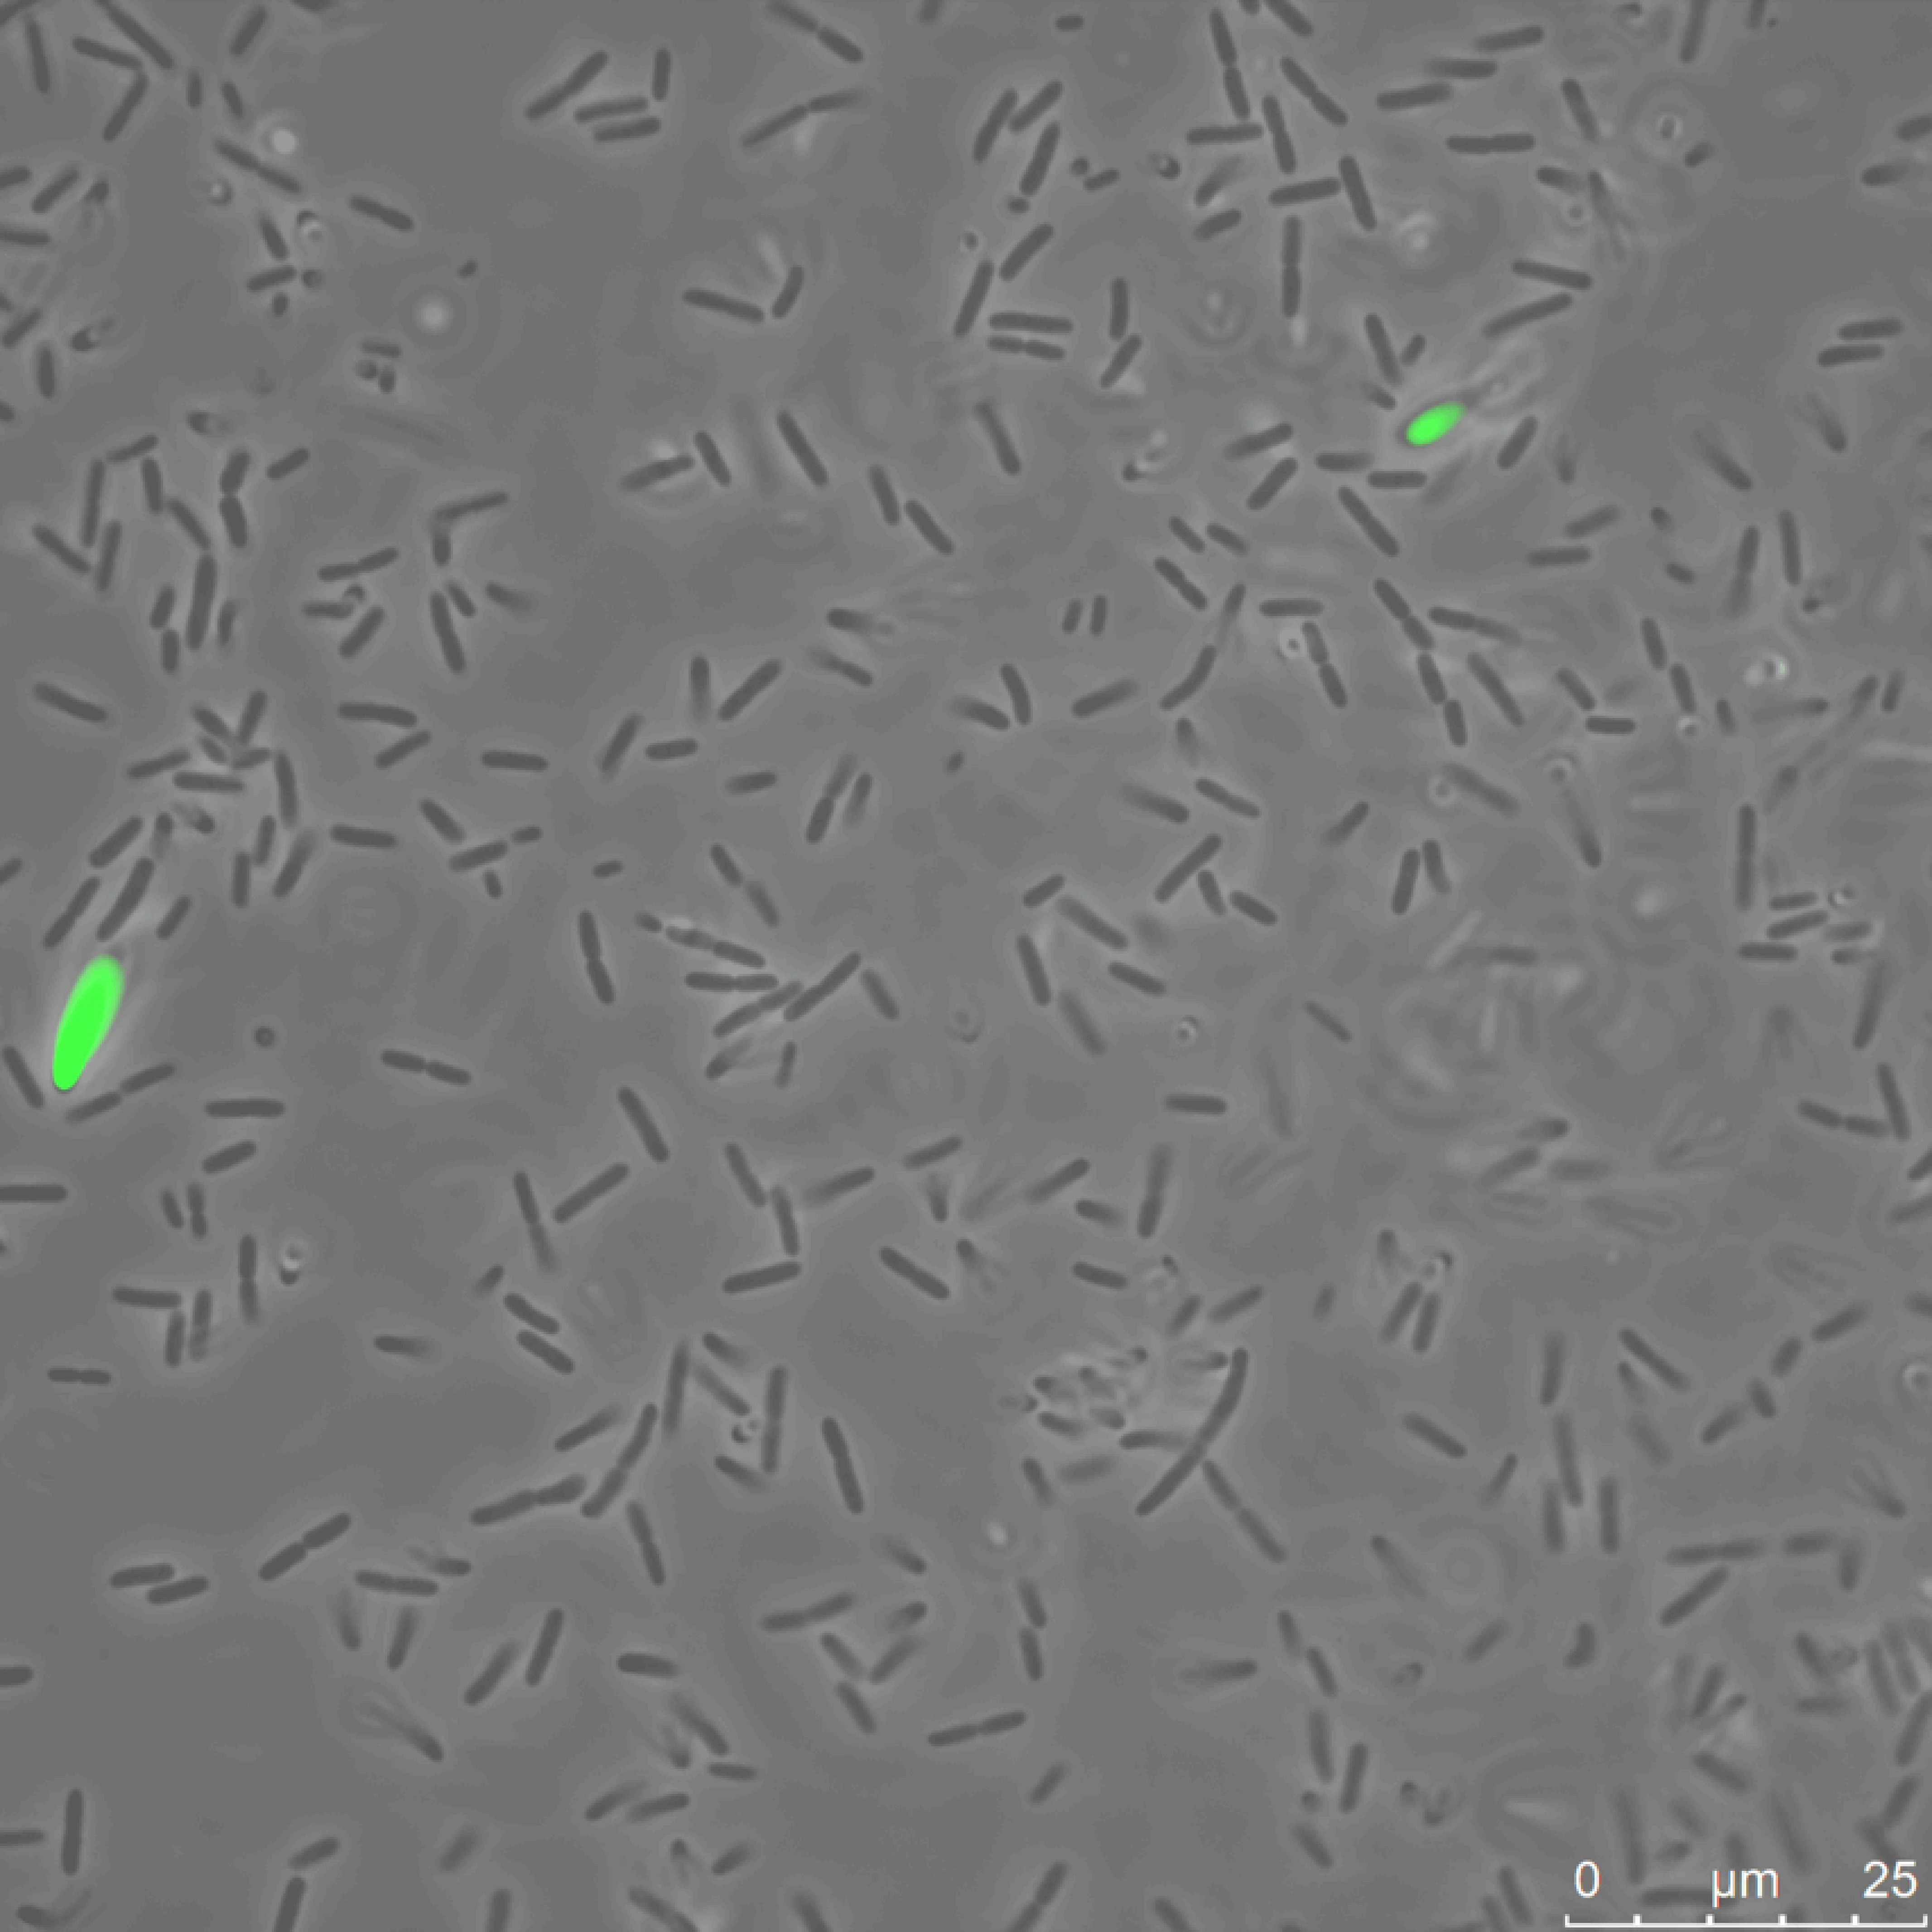
\includegraphics{THAIU1_1_GREEN-crunch-lighter-resample.pdf} &%
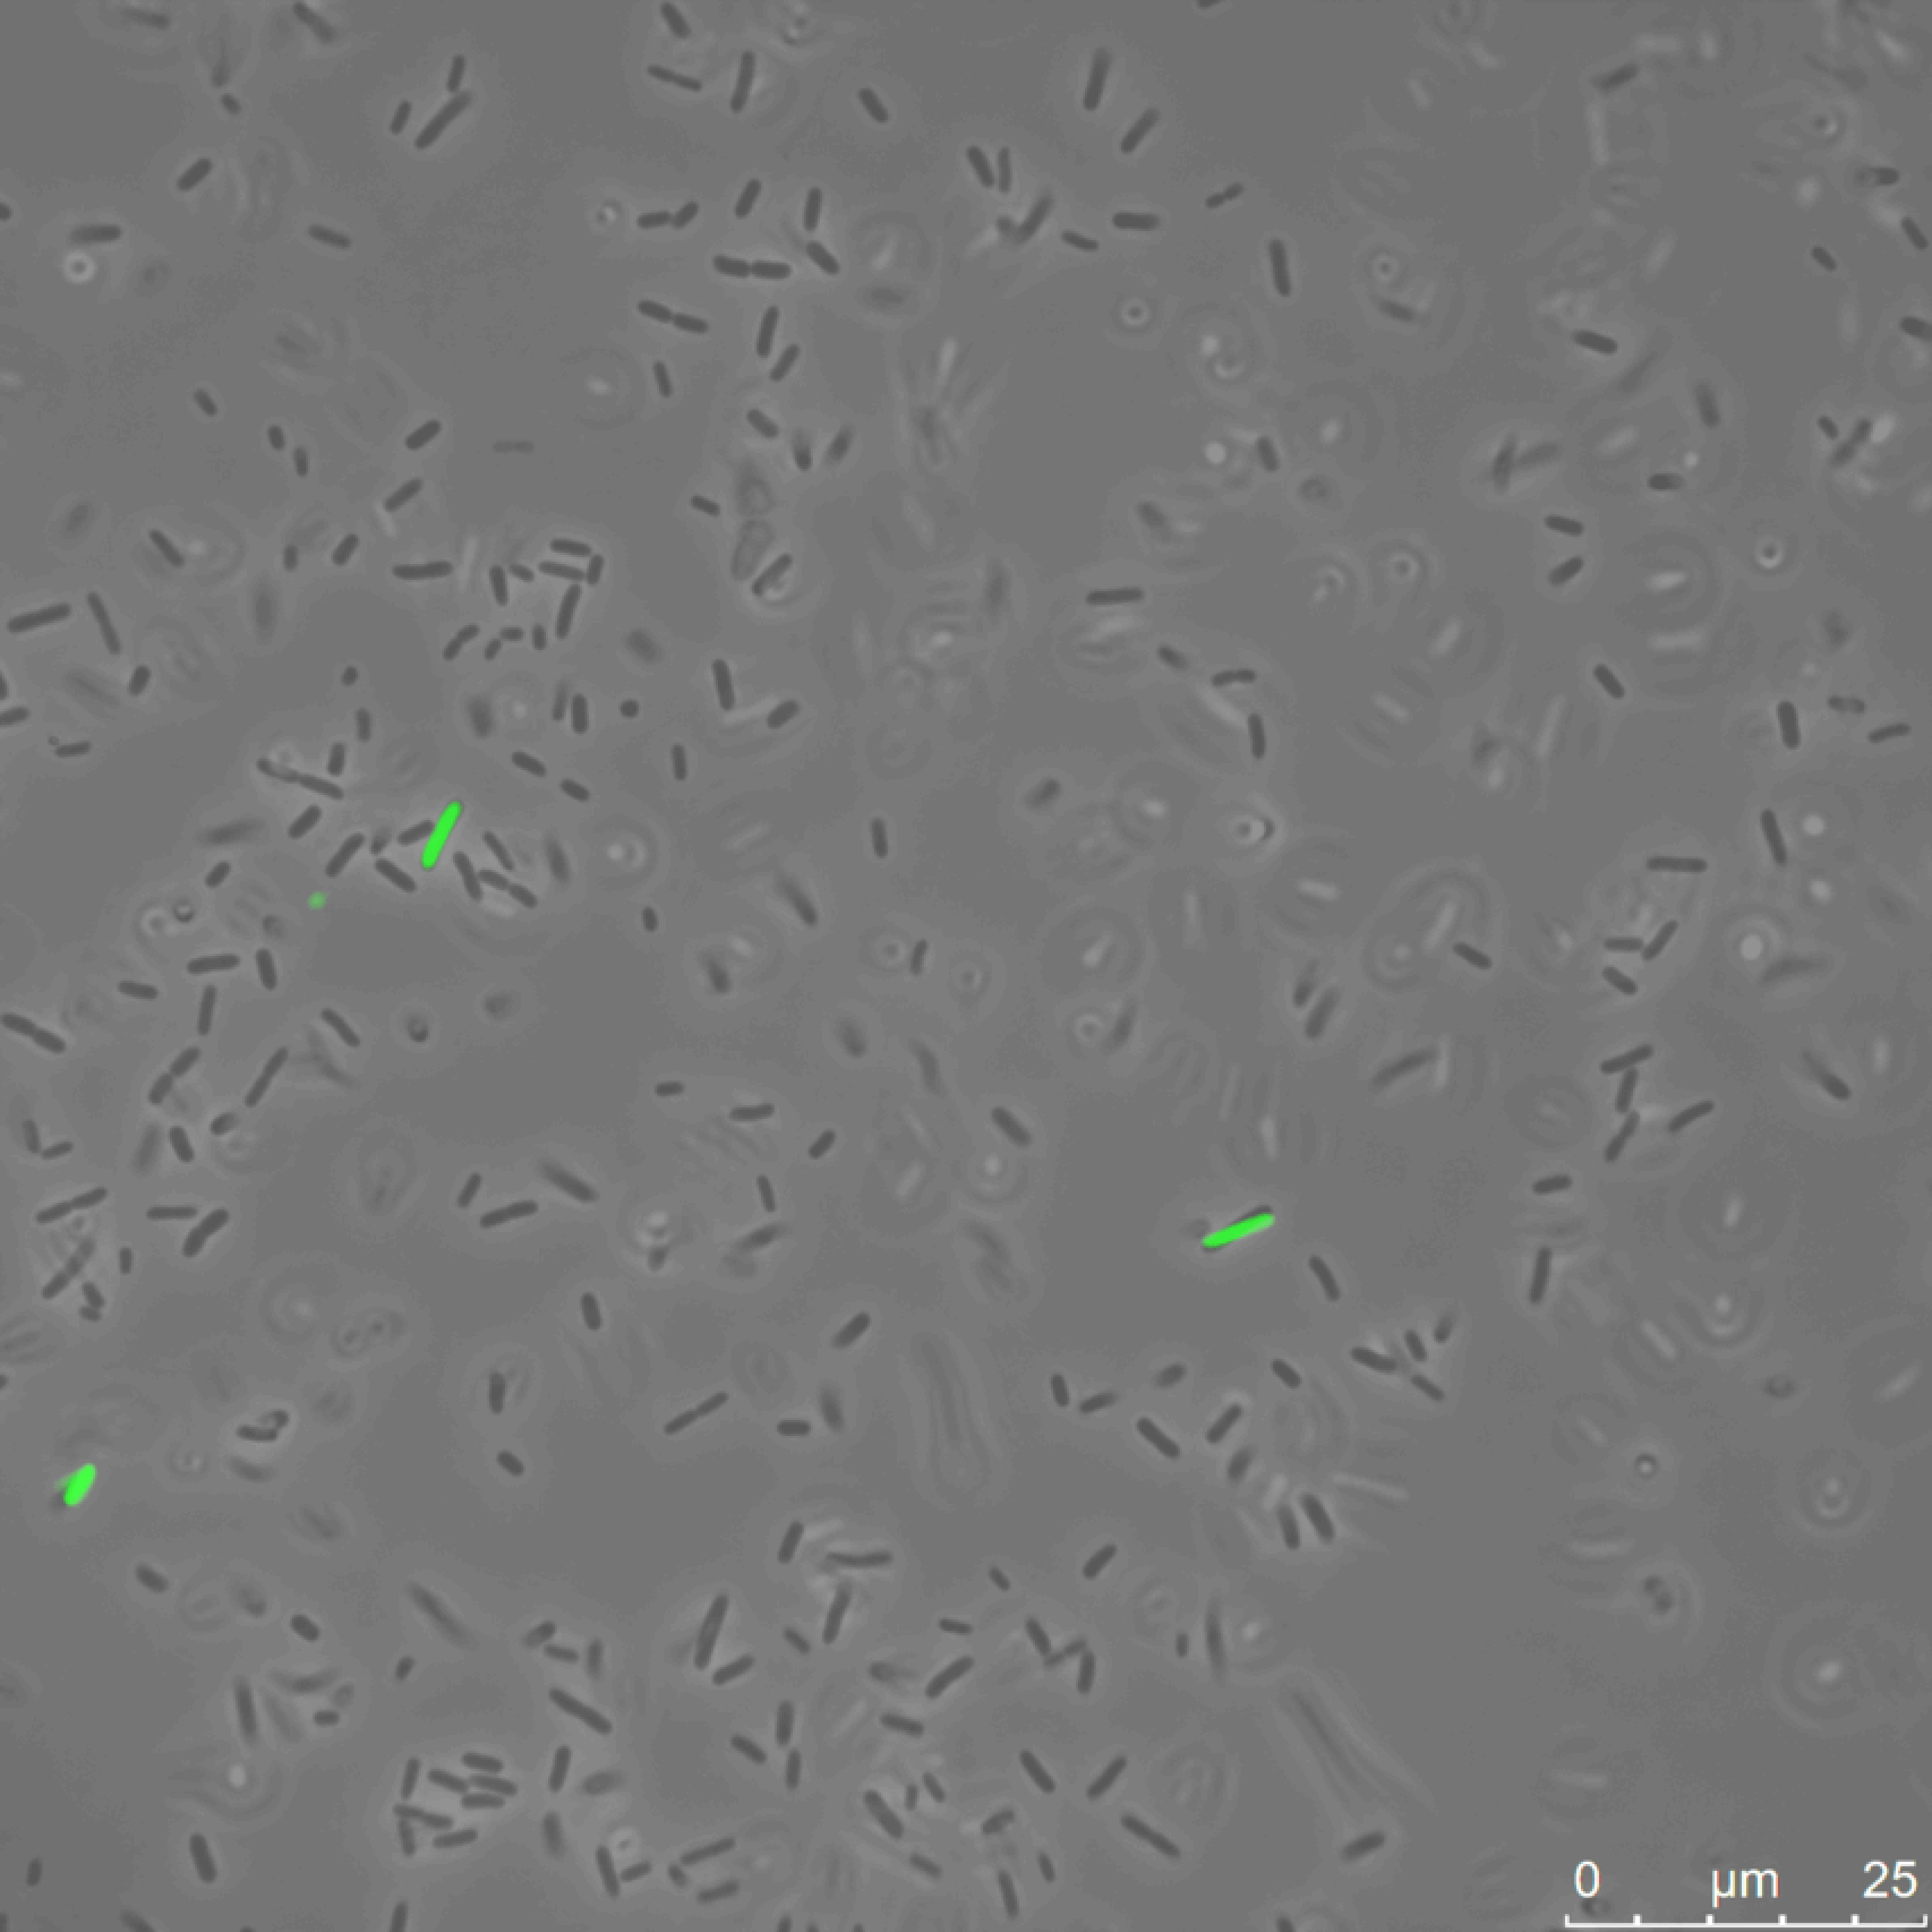
\includegraphics{THAIU1_5HR_5_GREEN-crunch-lighter-resample.pdf} &%
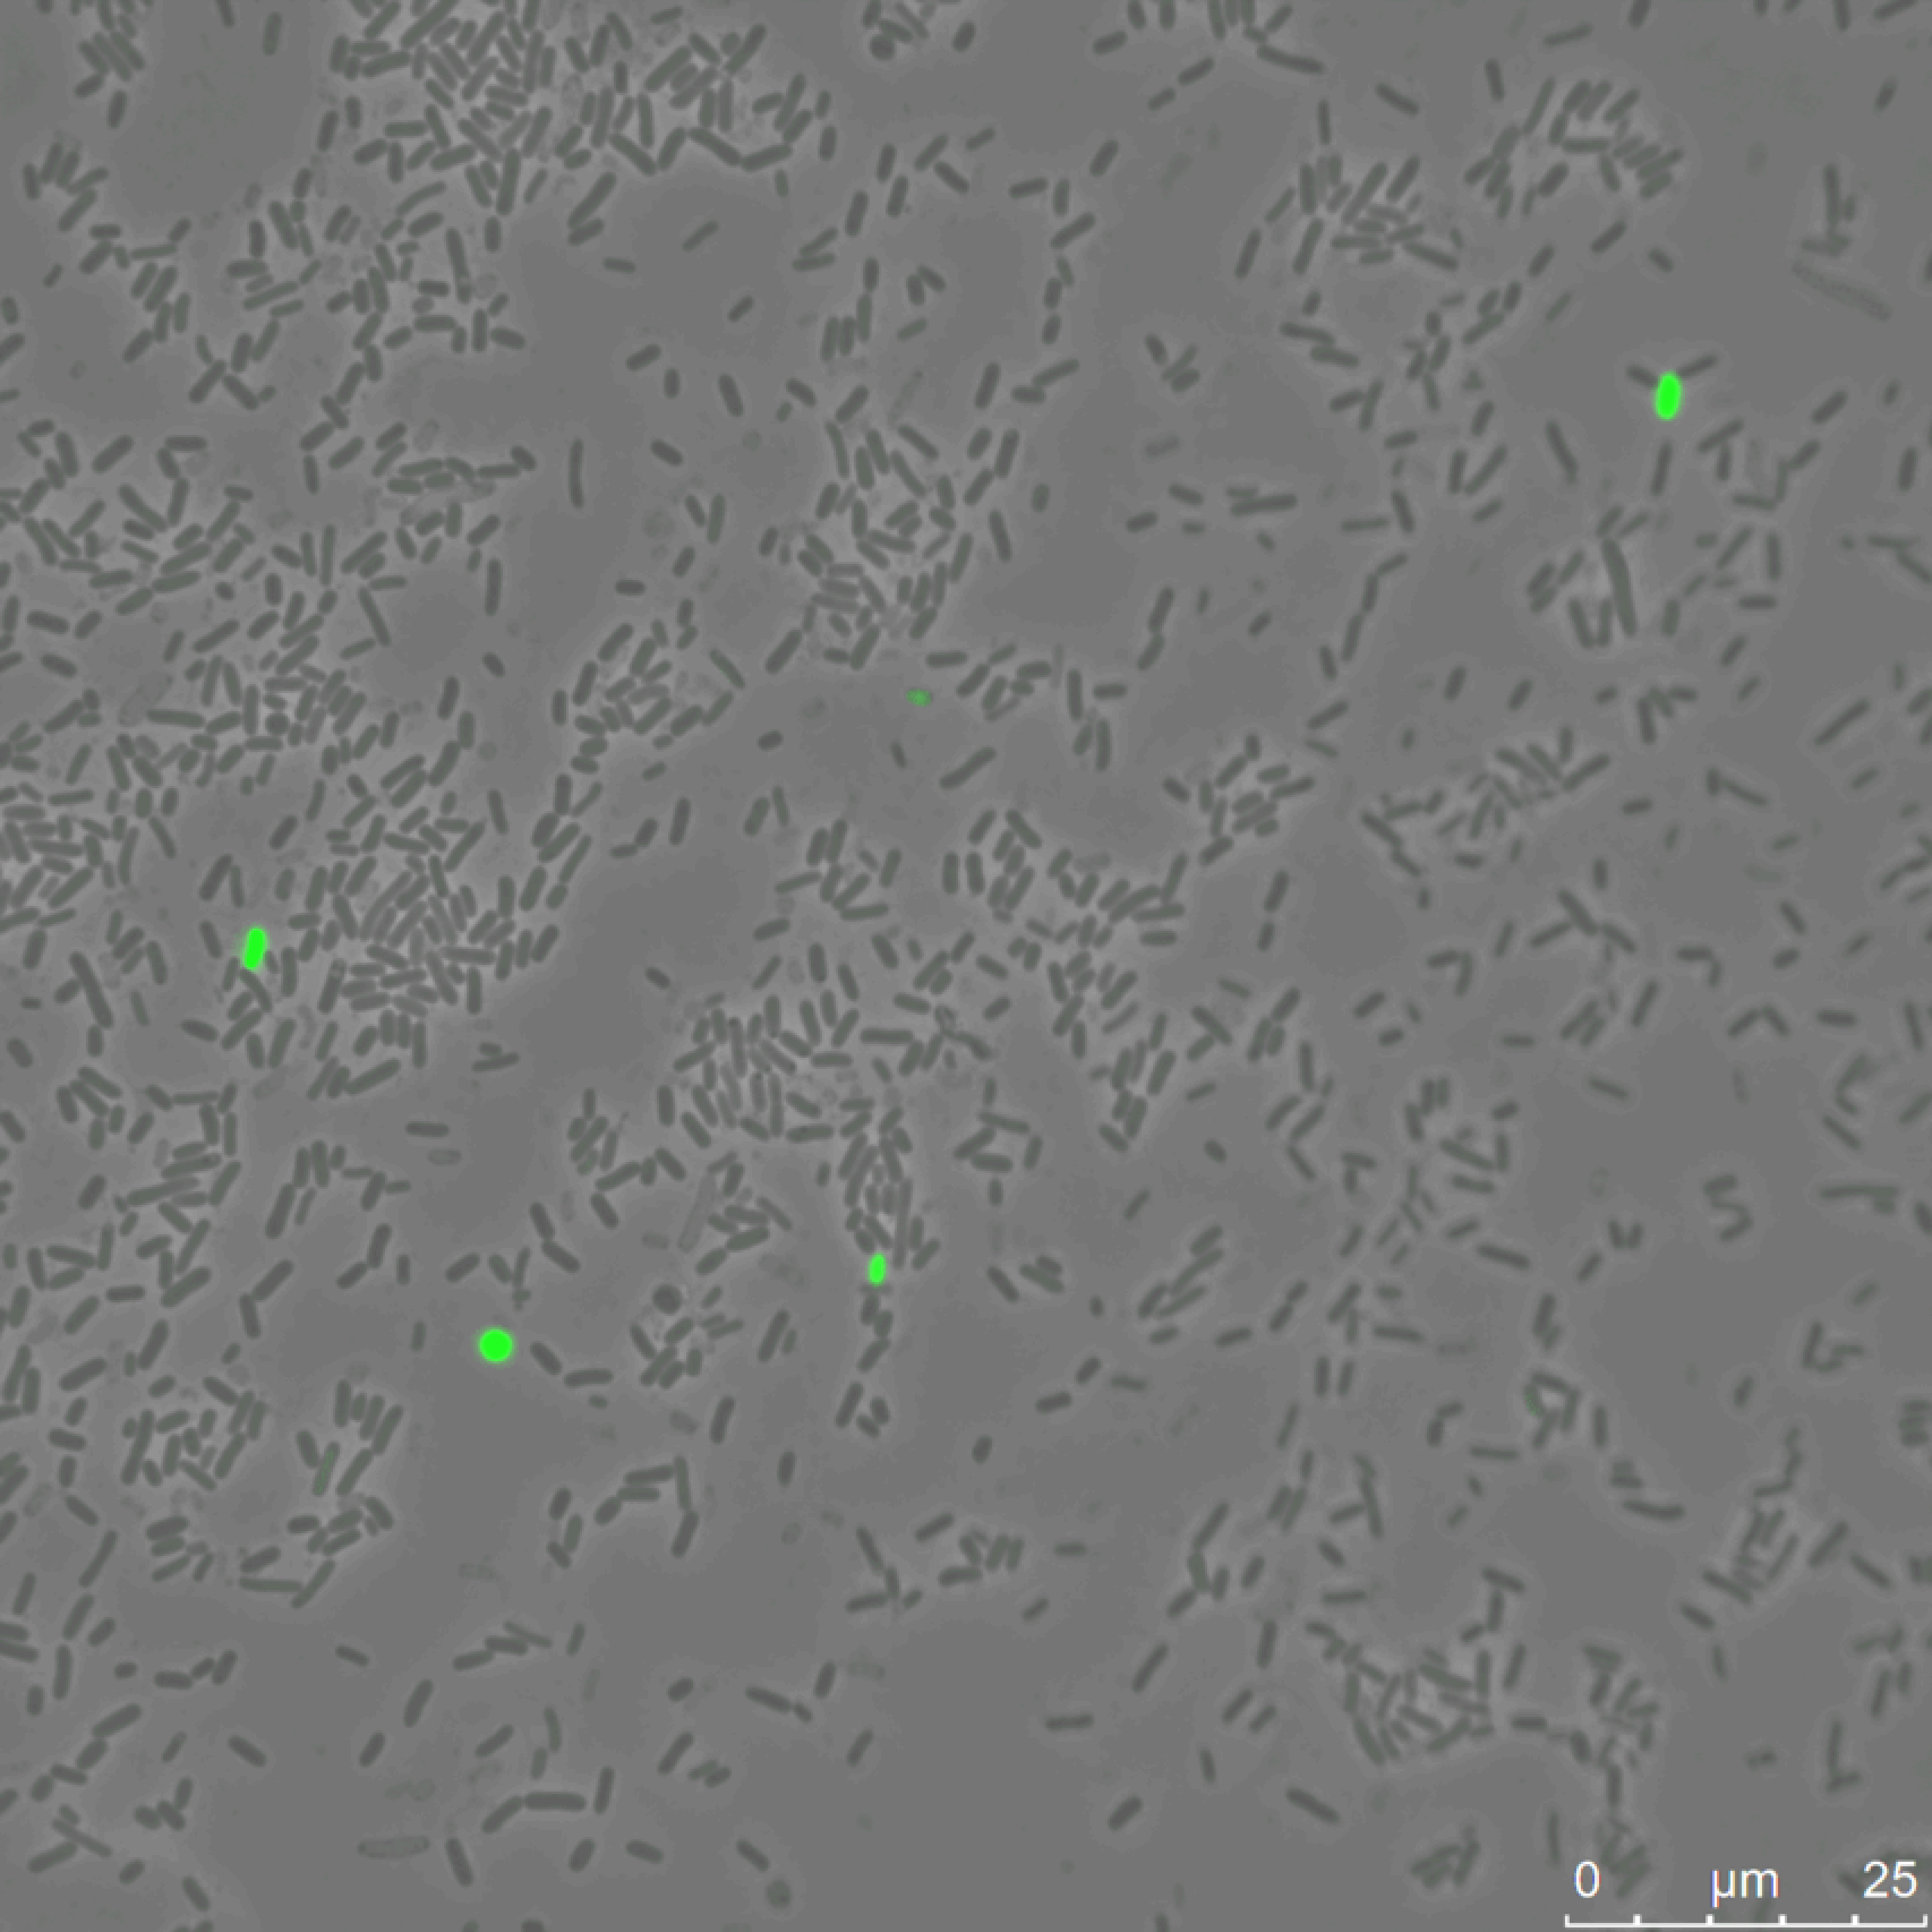
\includegraphics{THAIU1_24HR_1_GREEN-crunch-lighter-resample.pdf} &%
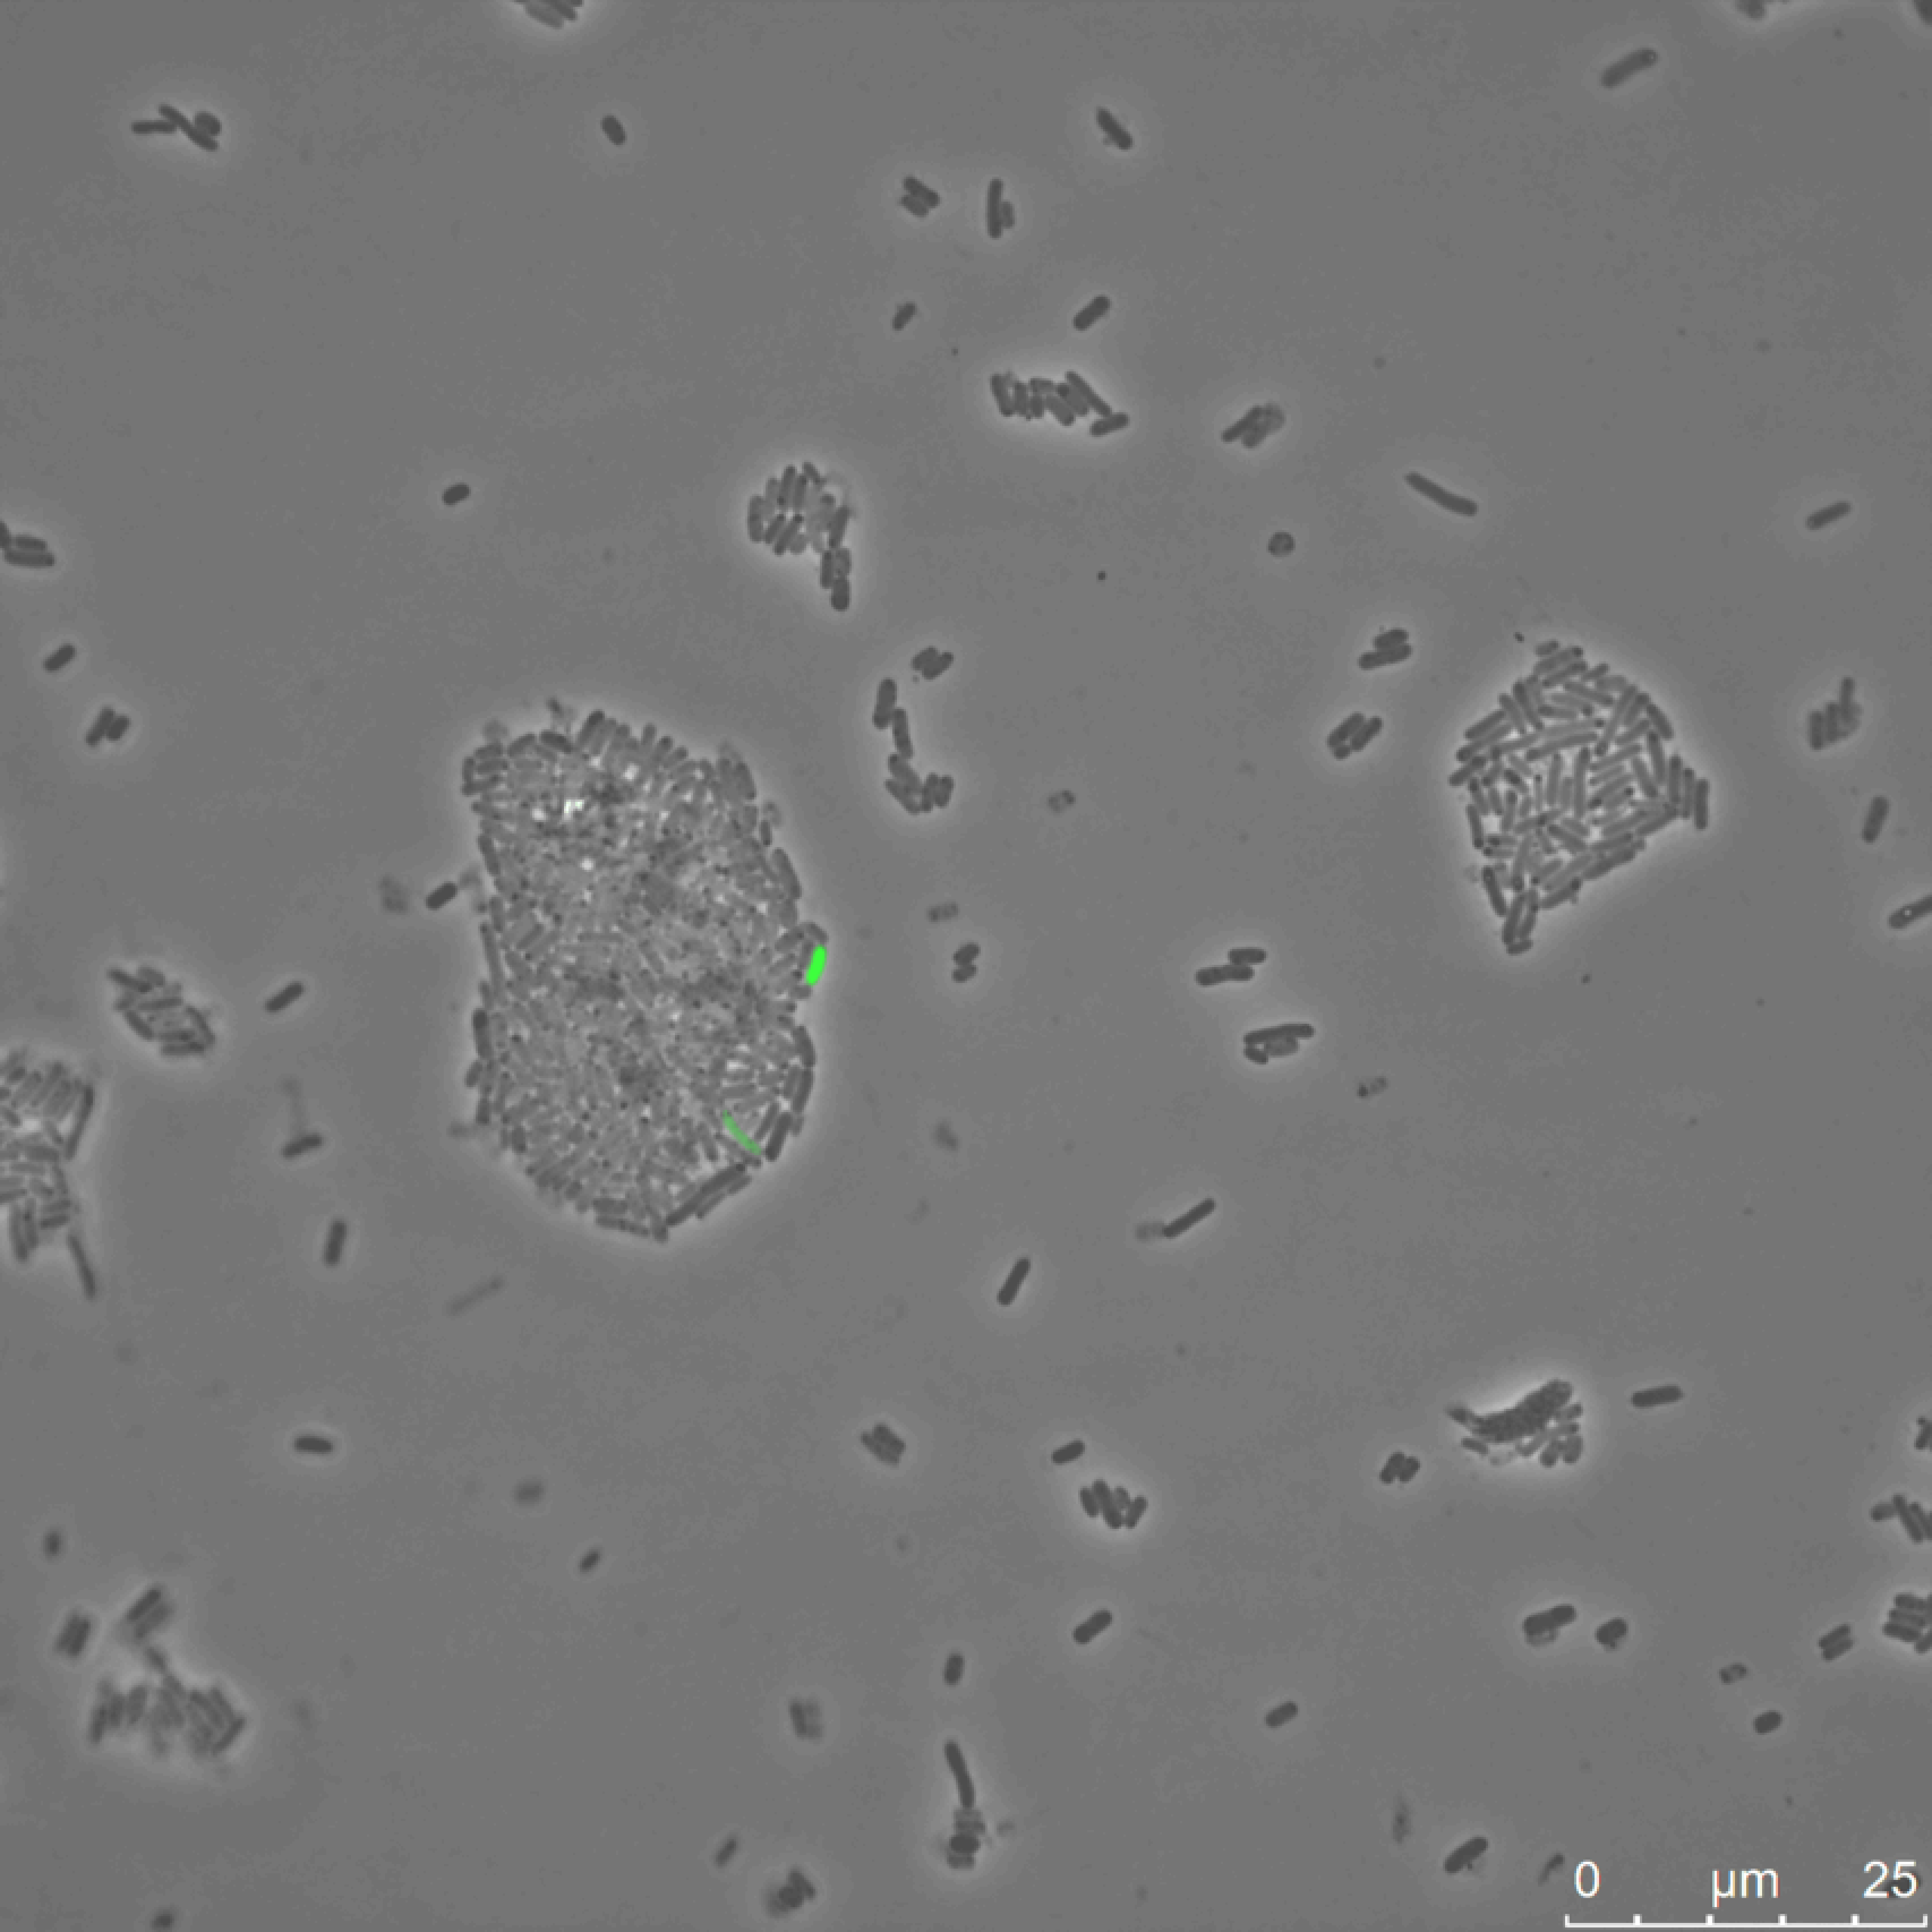
\includegraphics{THAIU1_72HR_1_GREEN-crunch-lighter-resample.pdf} \\[-0.5ex]

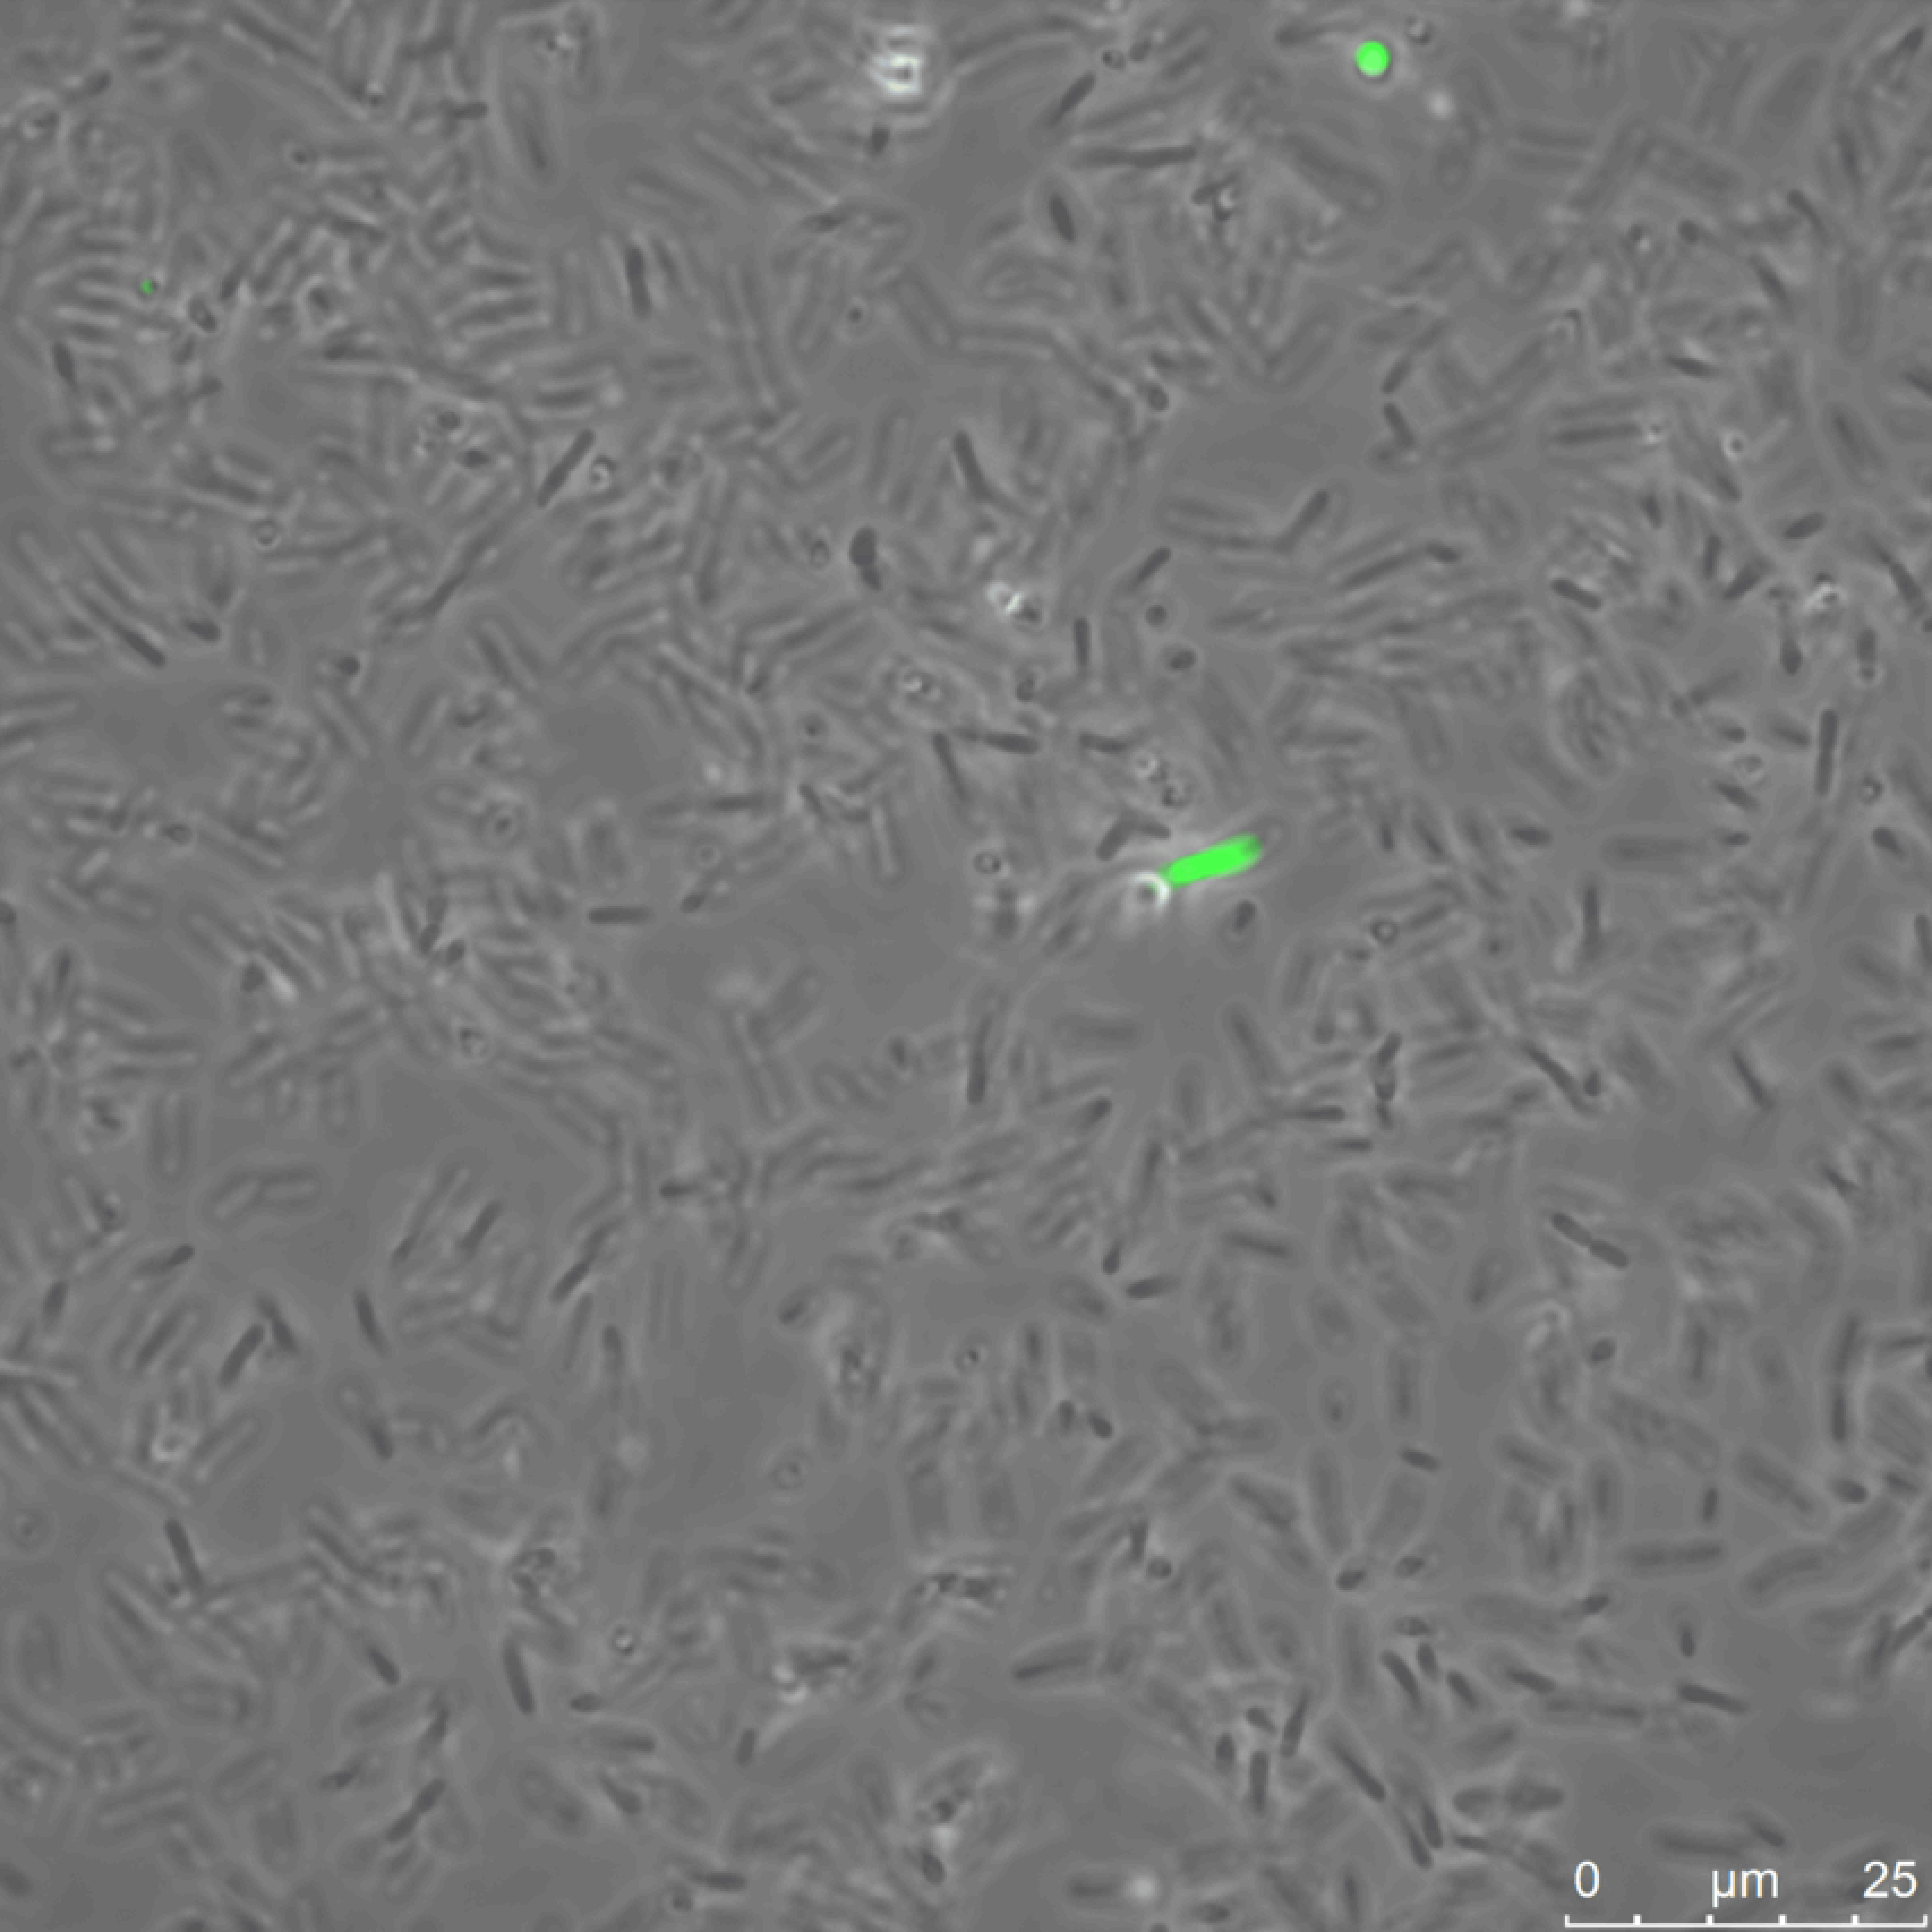
\includegraphics{THAIU1_2_GREEN-crunch-lighter-resample.pdf} &%
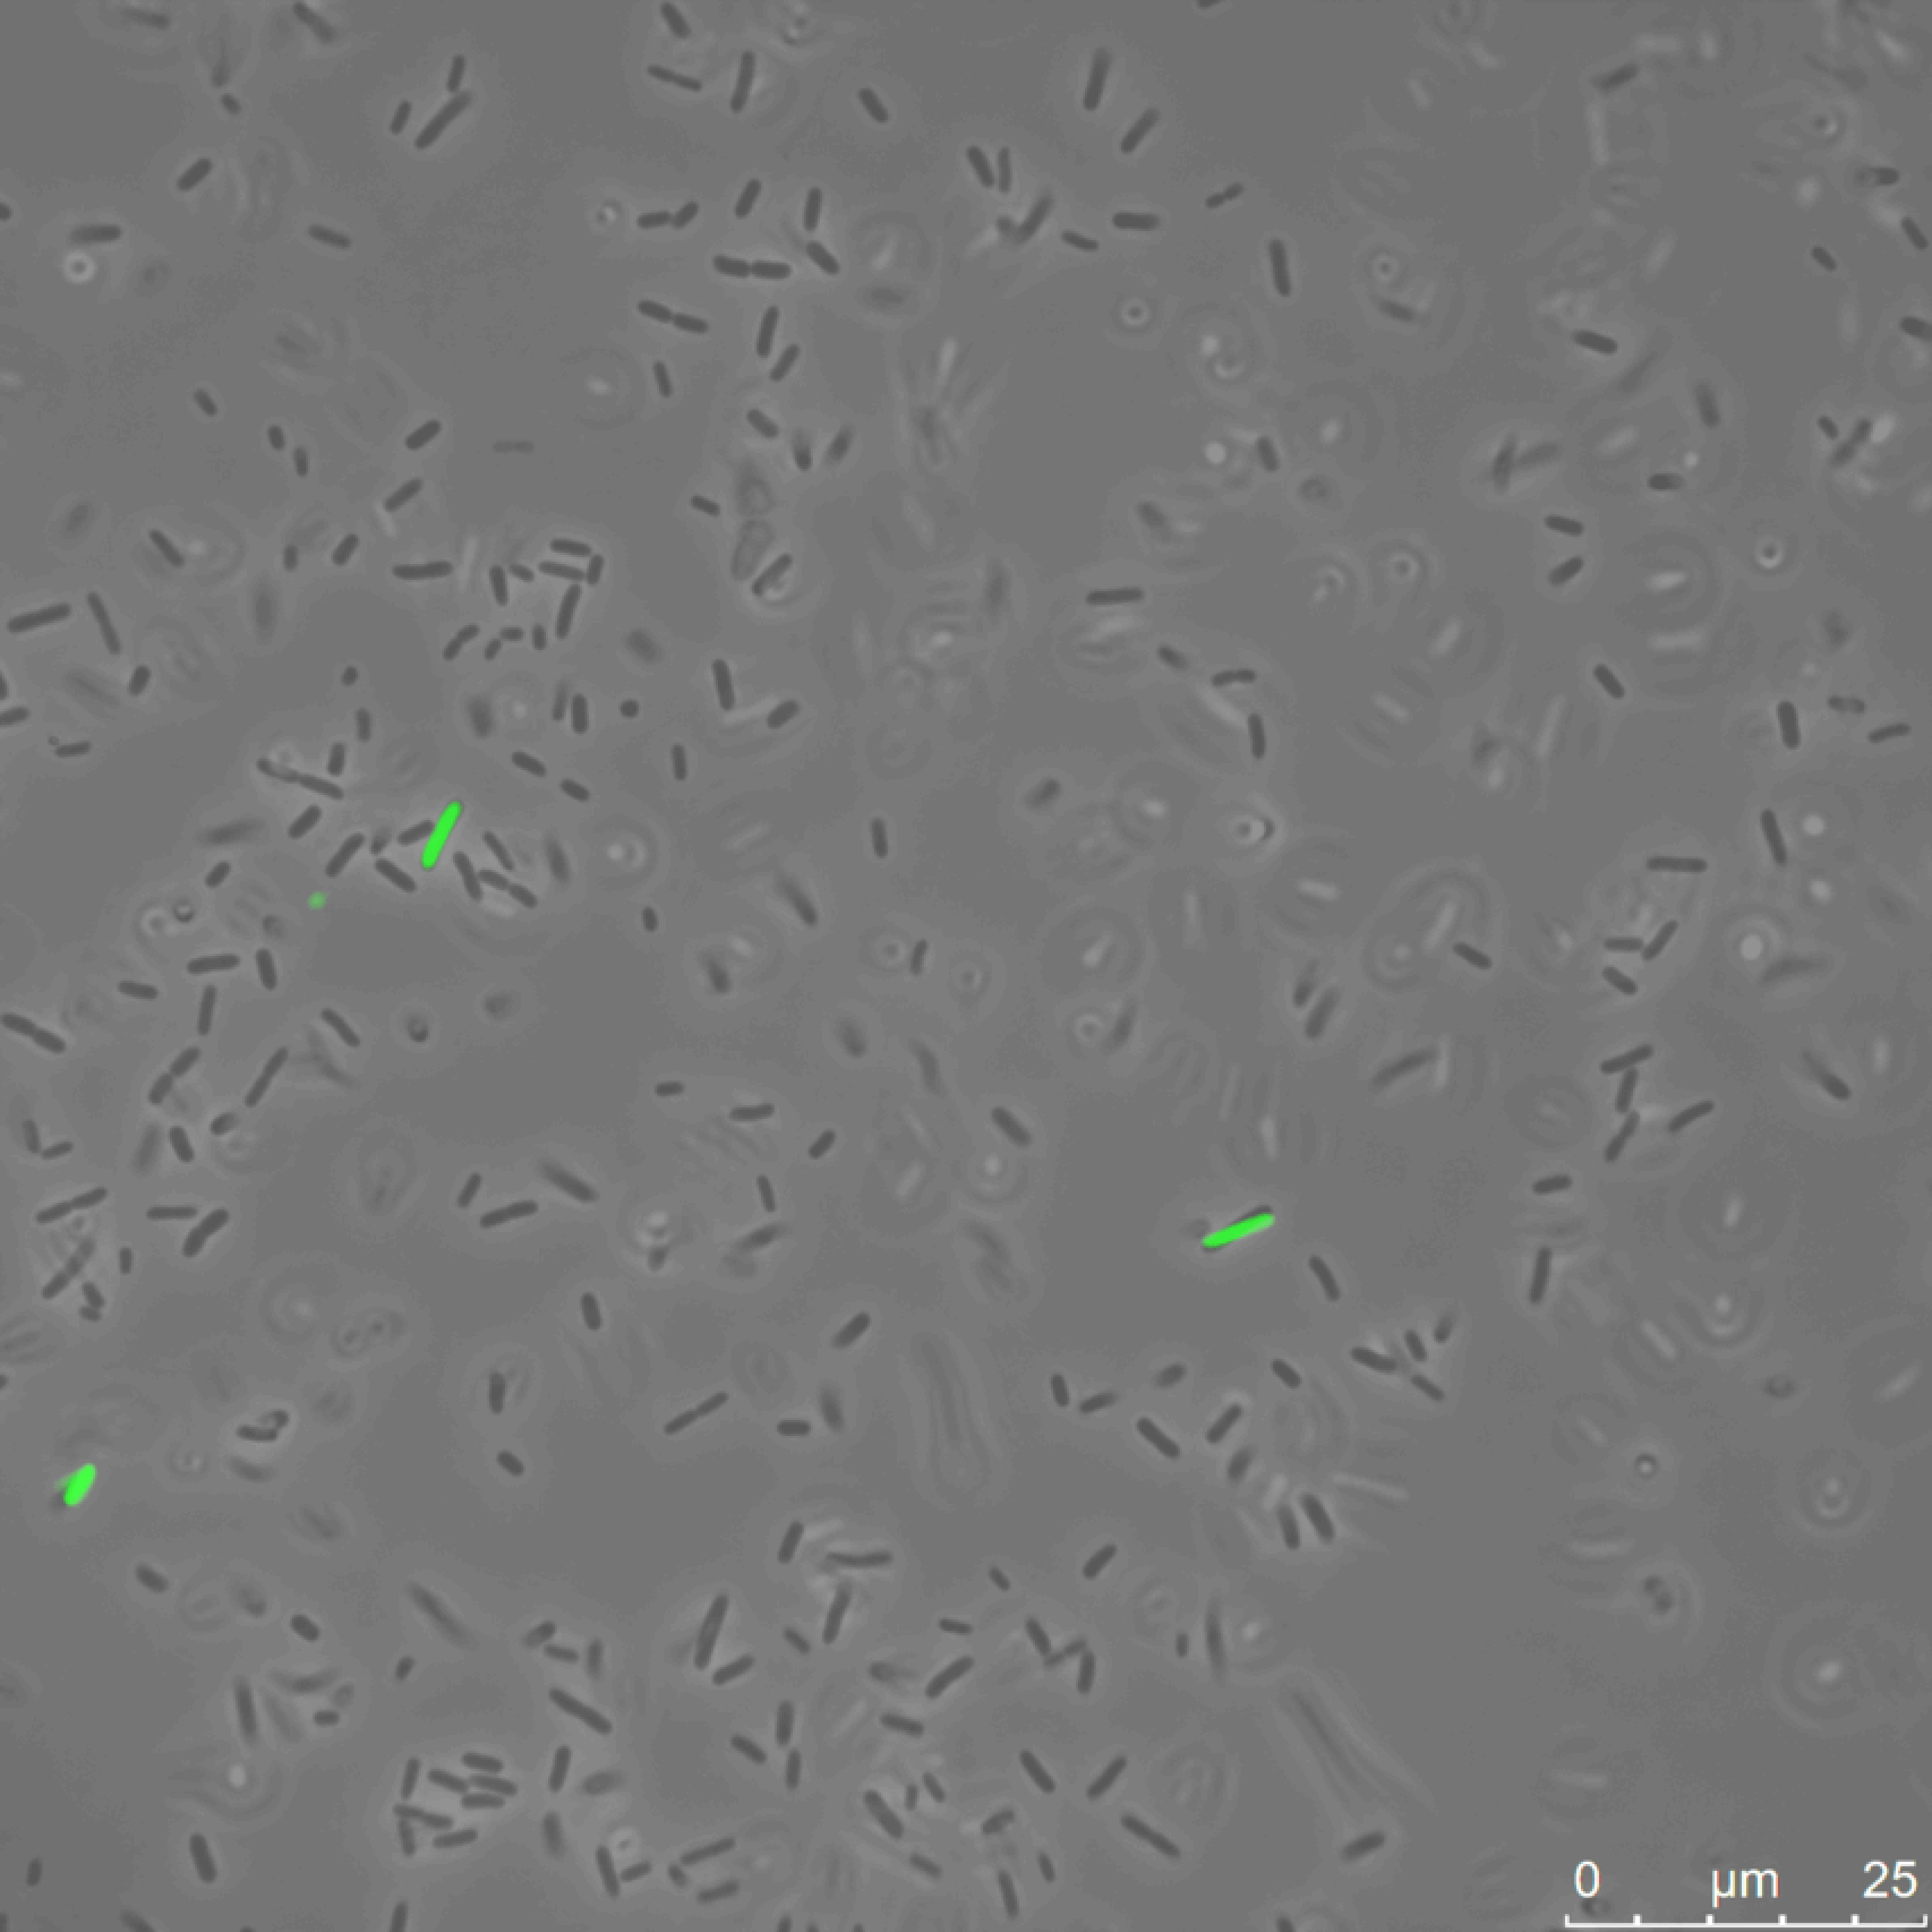
\includegraphics{THAIU1_5HR_5_GREEN-crunch-lighter-resample.pdf} &%
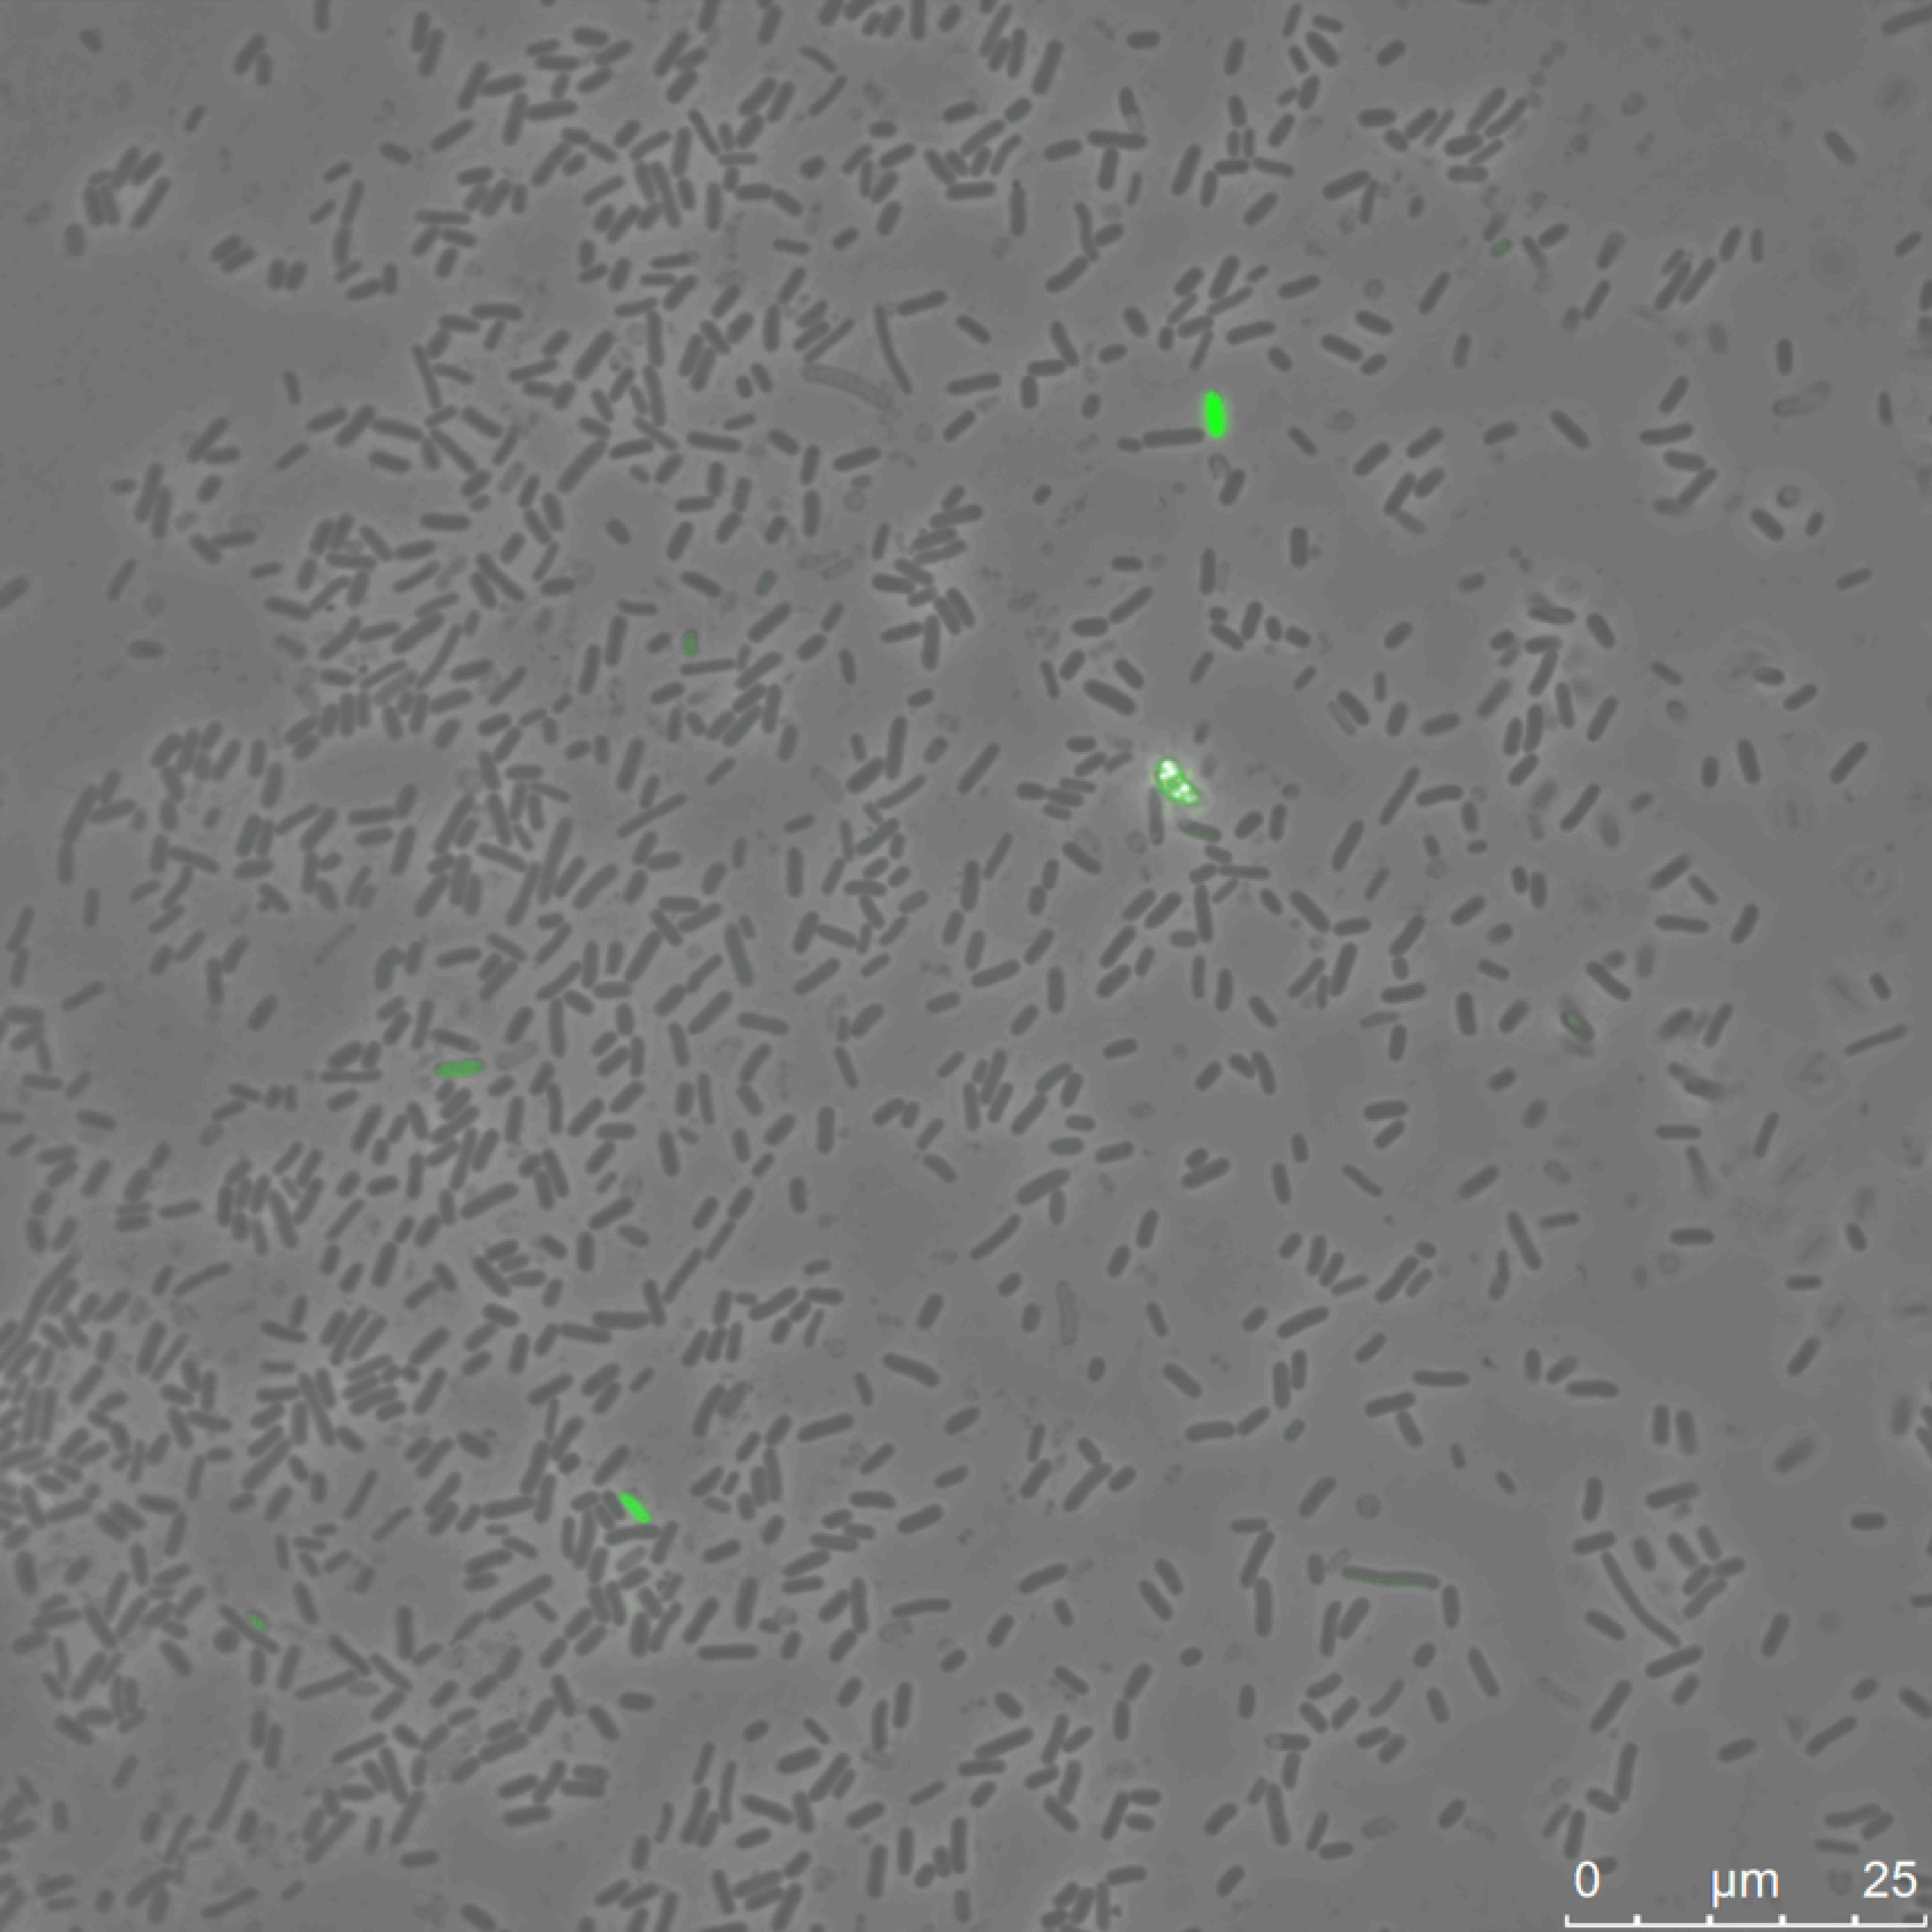
\includegraphics{THAIU1_24HR_2_GREEN-crunch-lighter-resample.pdf} &%
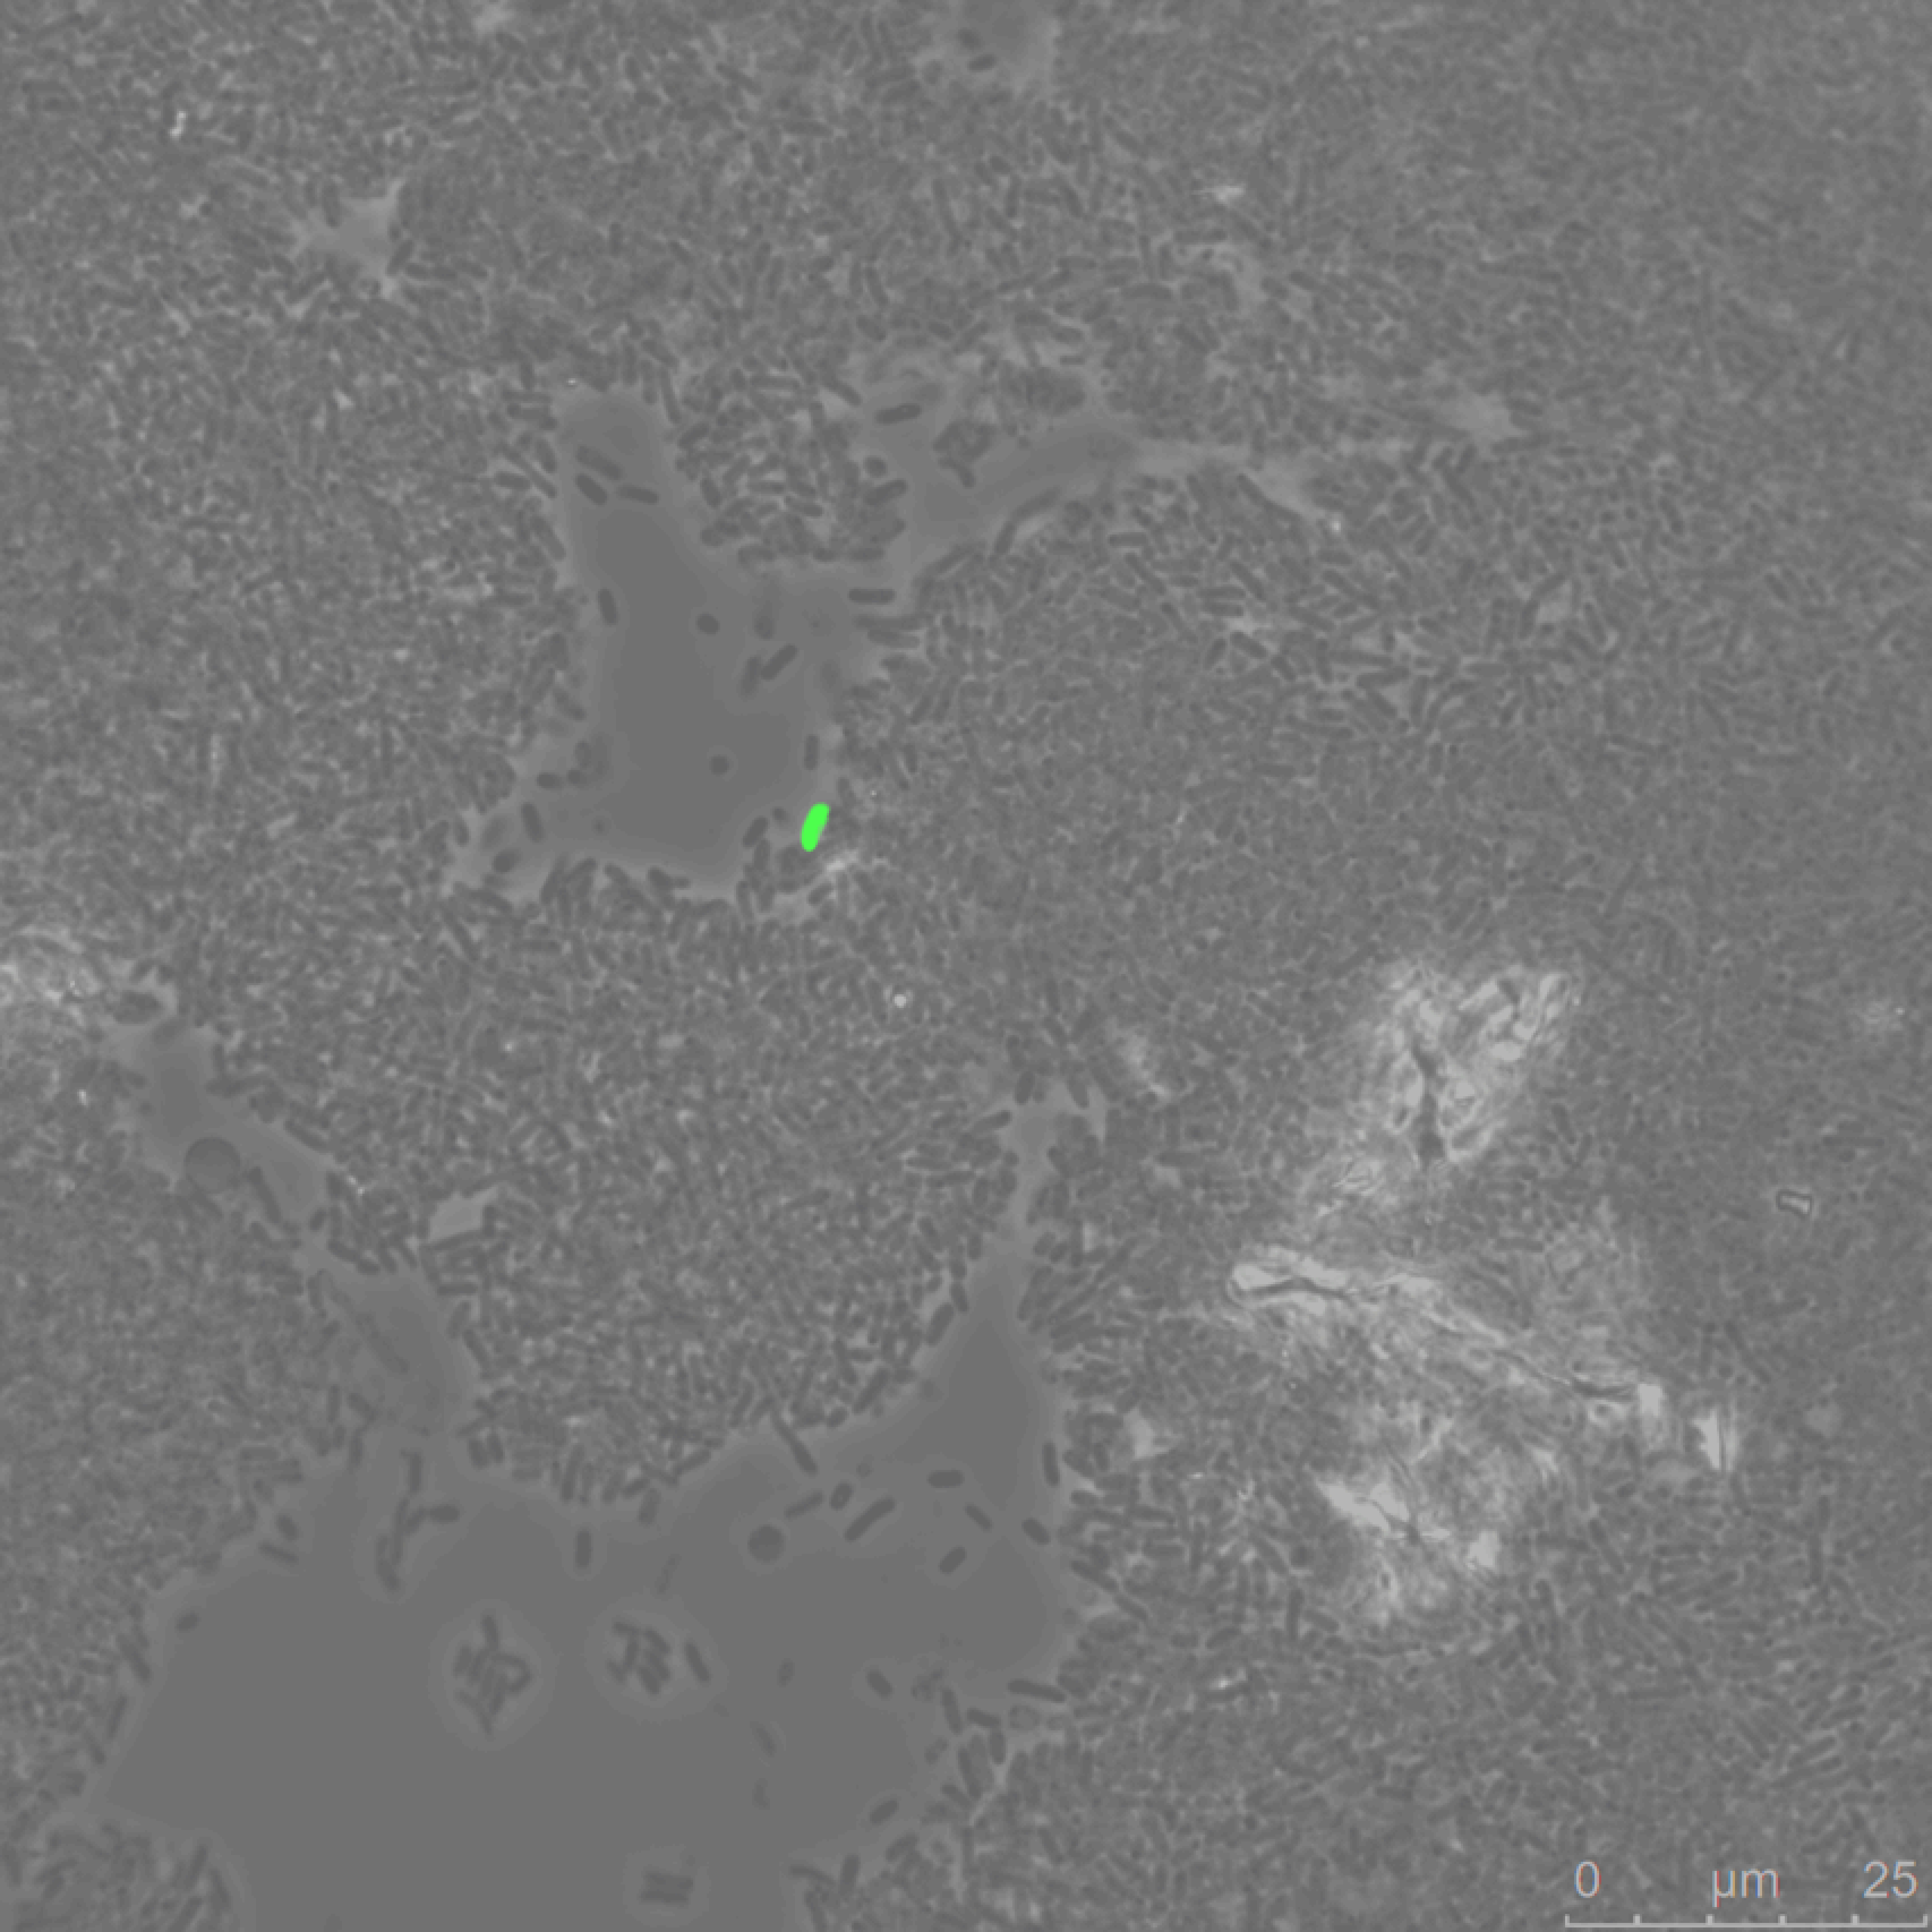
\includegraphics{THAIU1_72HR_2_GREEN-crunch-lighter-resample.pdf} \\[-0.5ex]

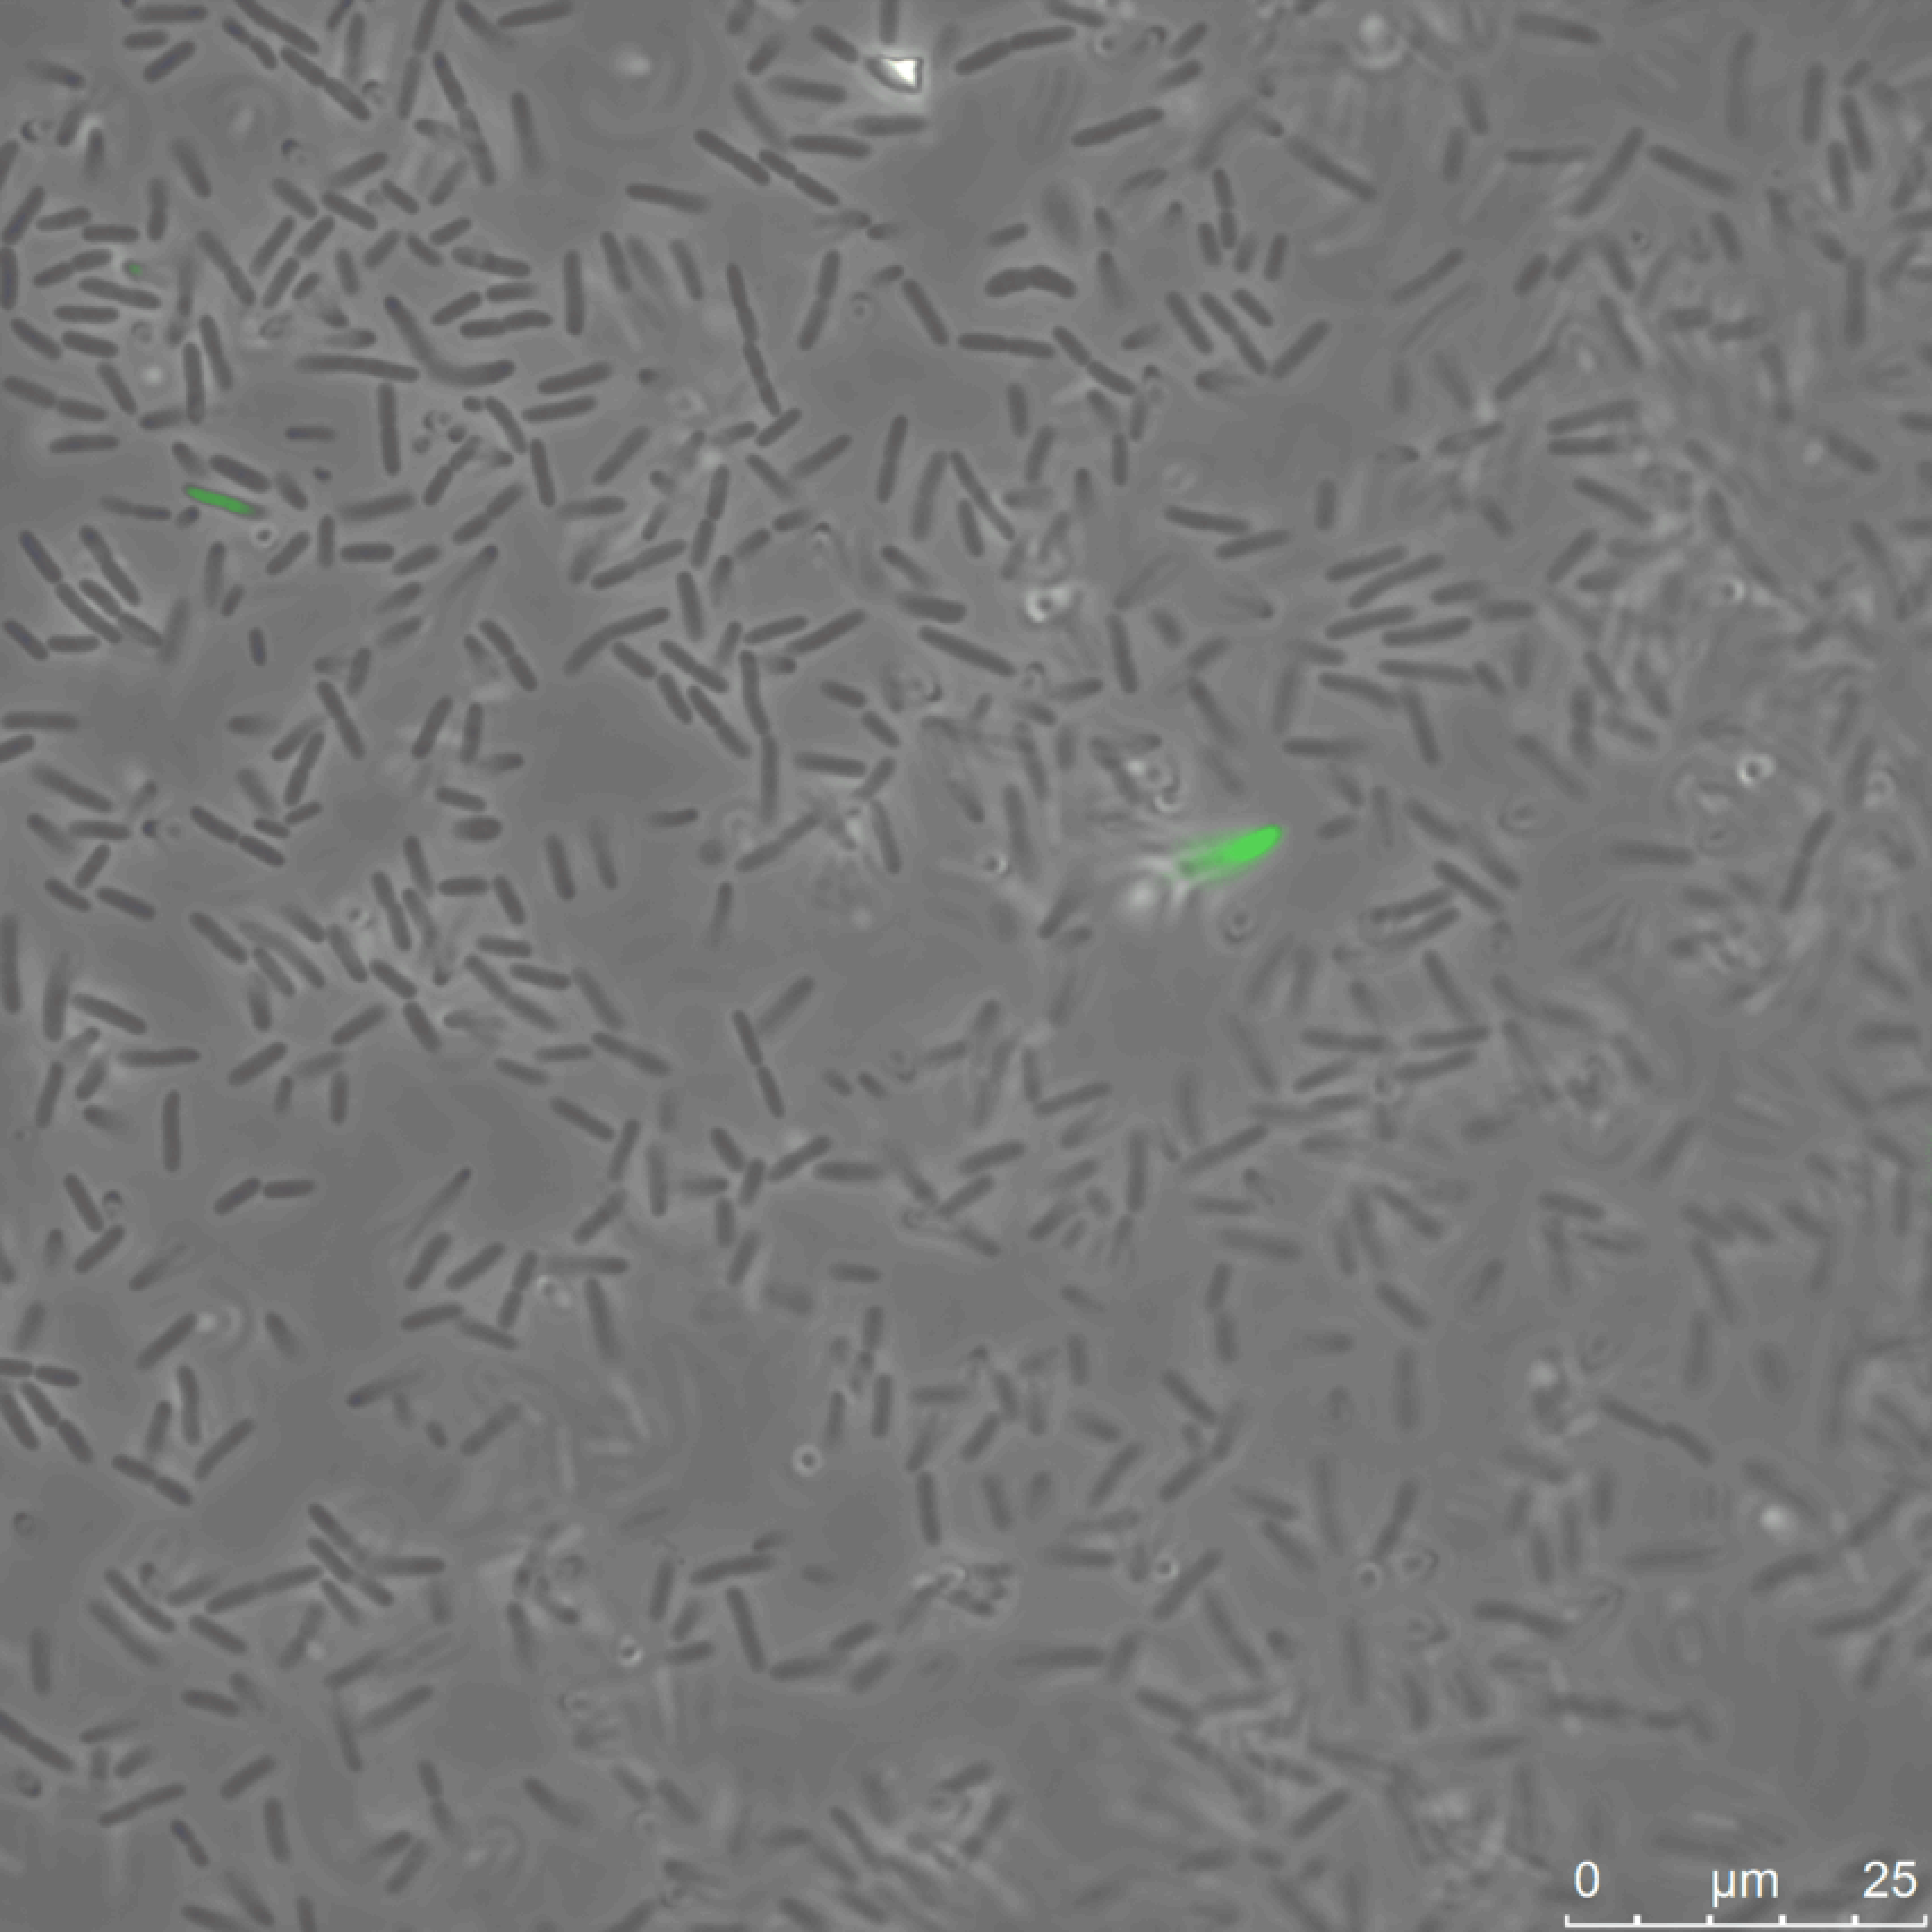
\includegraphics{THAIU1_3_GREEN-crunch-lighter-resample.pdf} &%
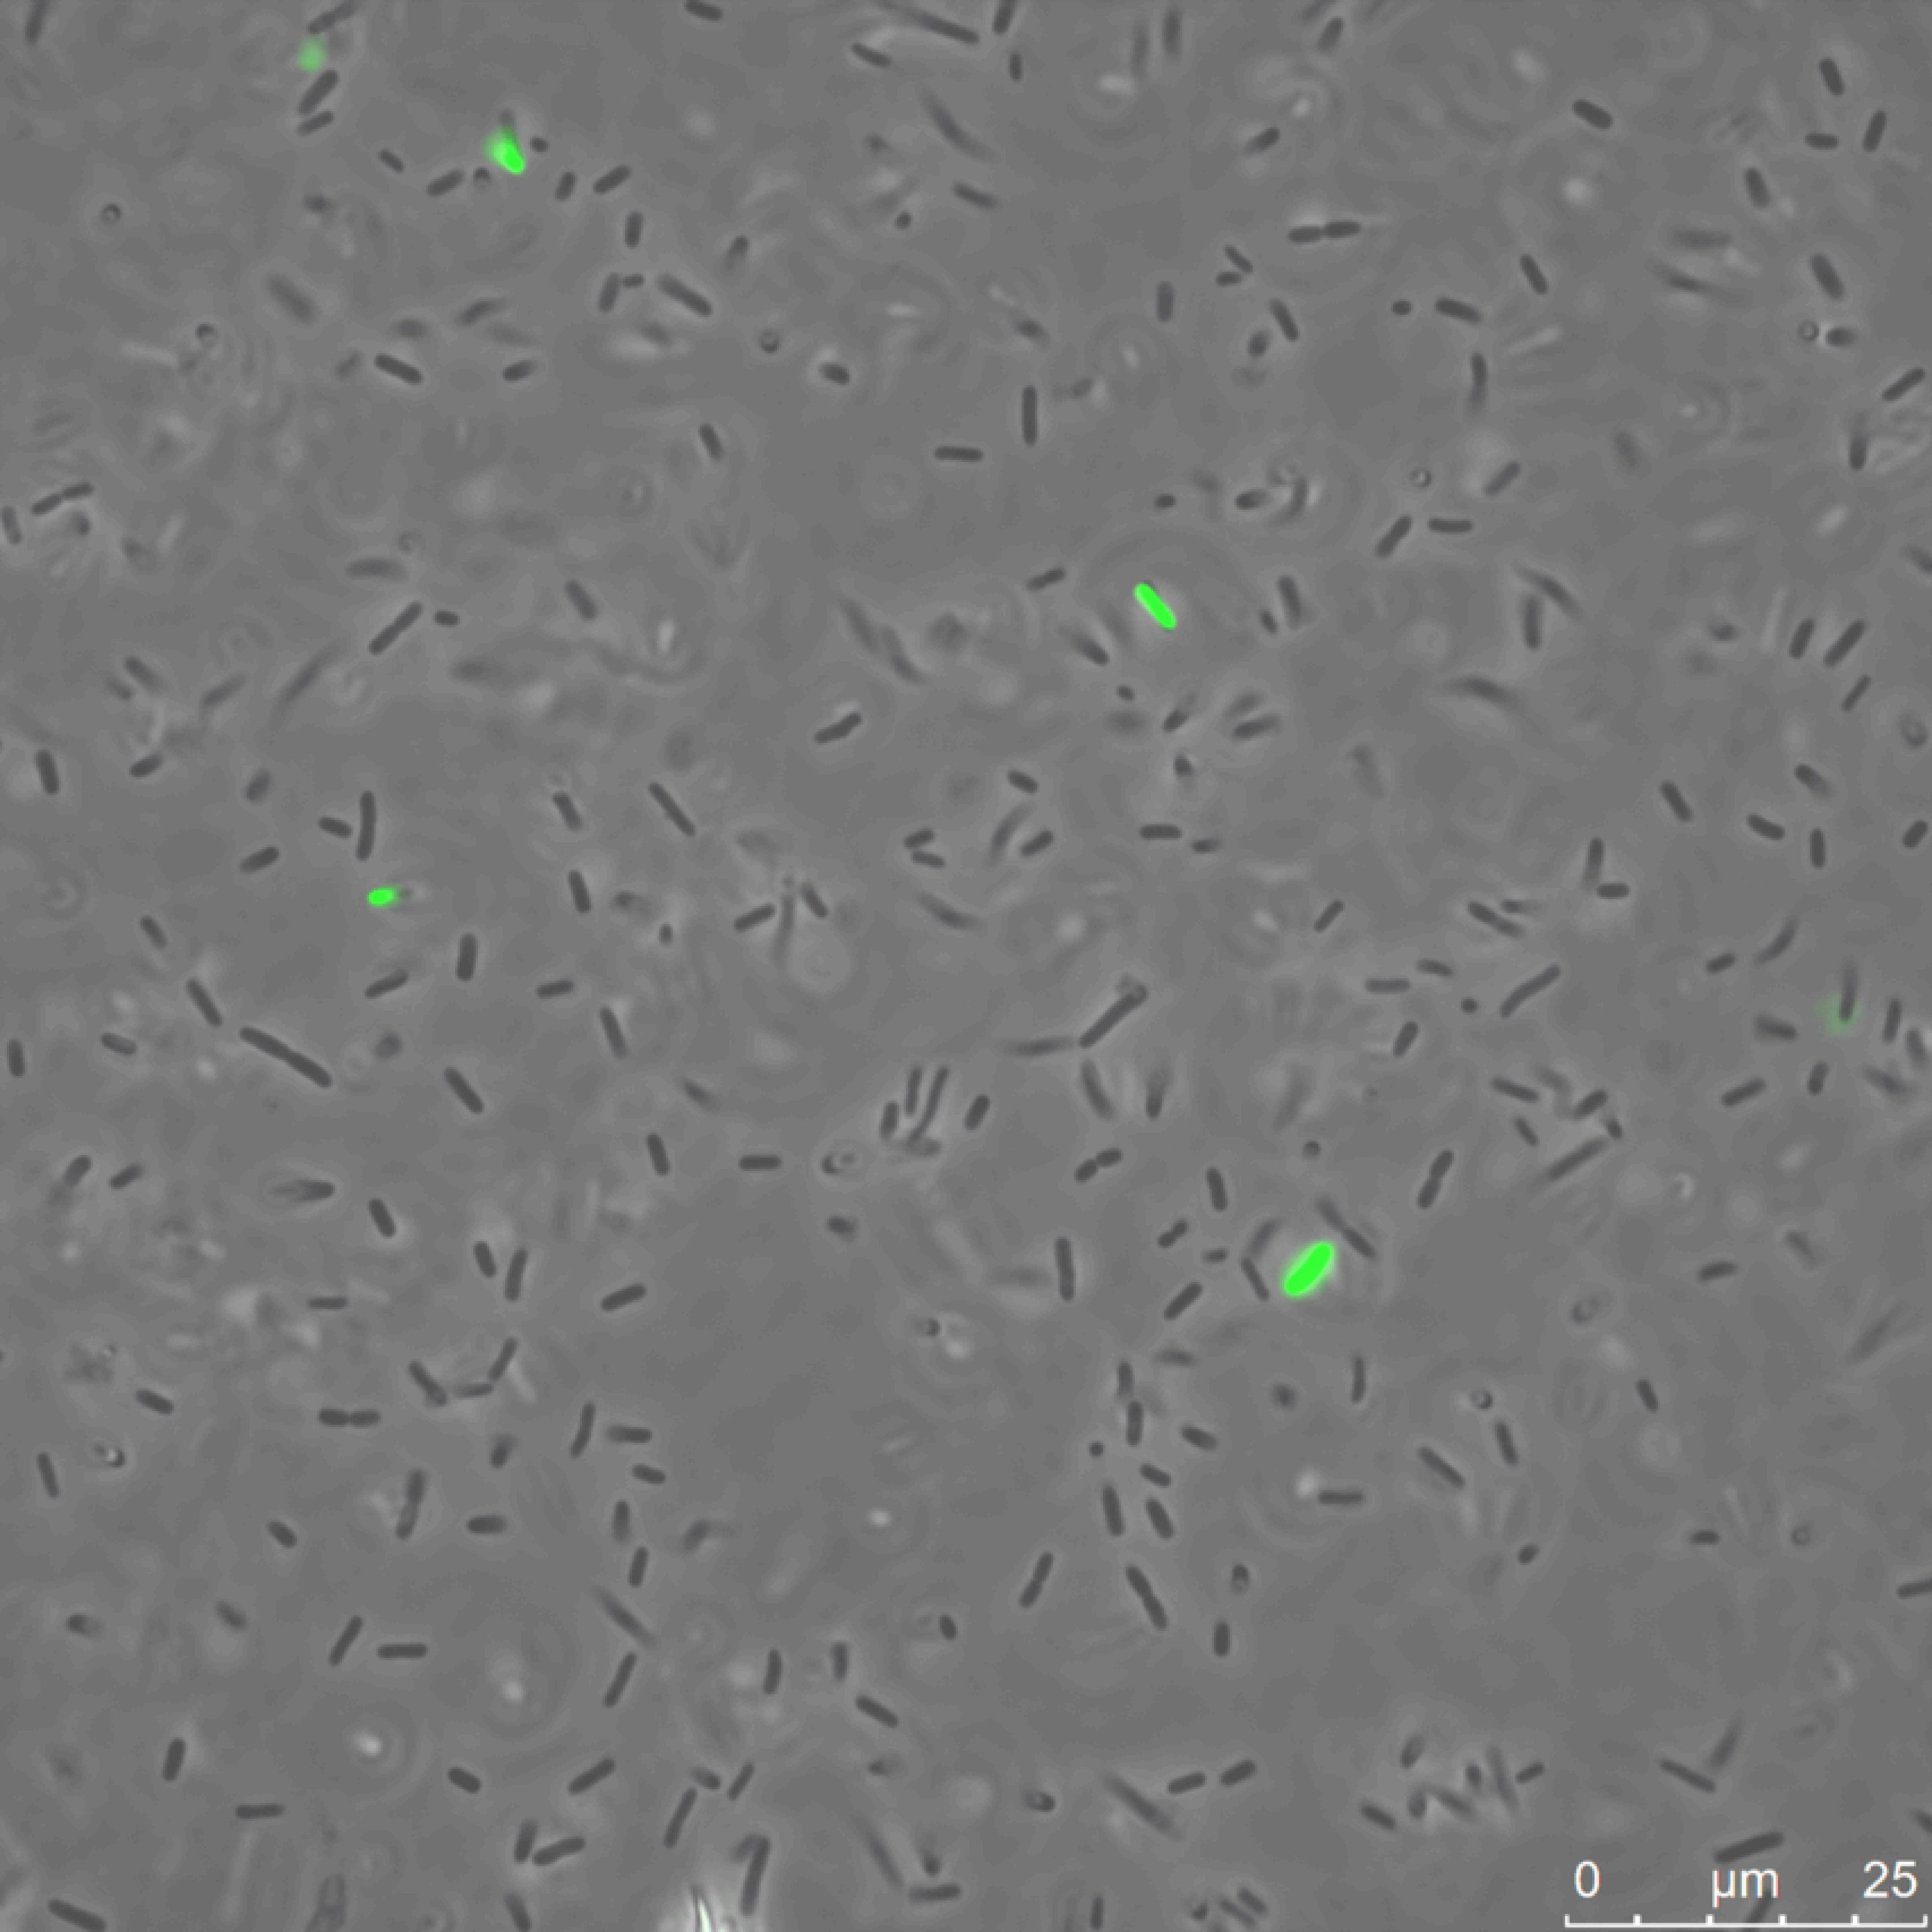
\includegraphics{THAIU1_5HR_3_GREEN-crunch-lighter-resample.pdf} &%
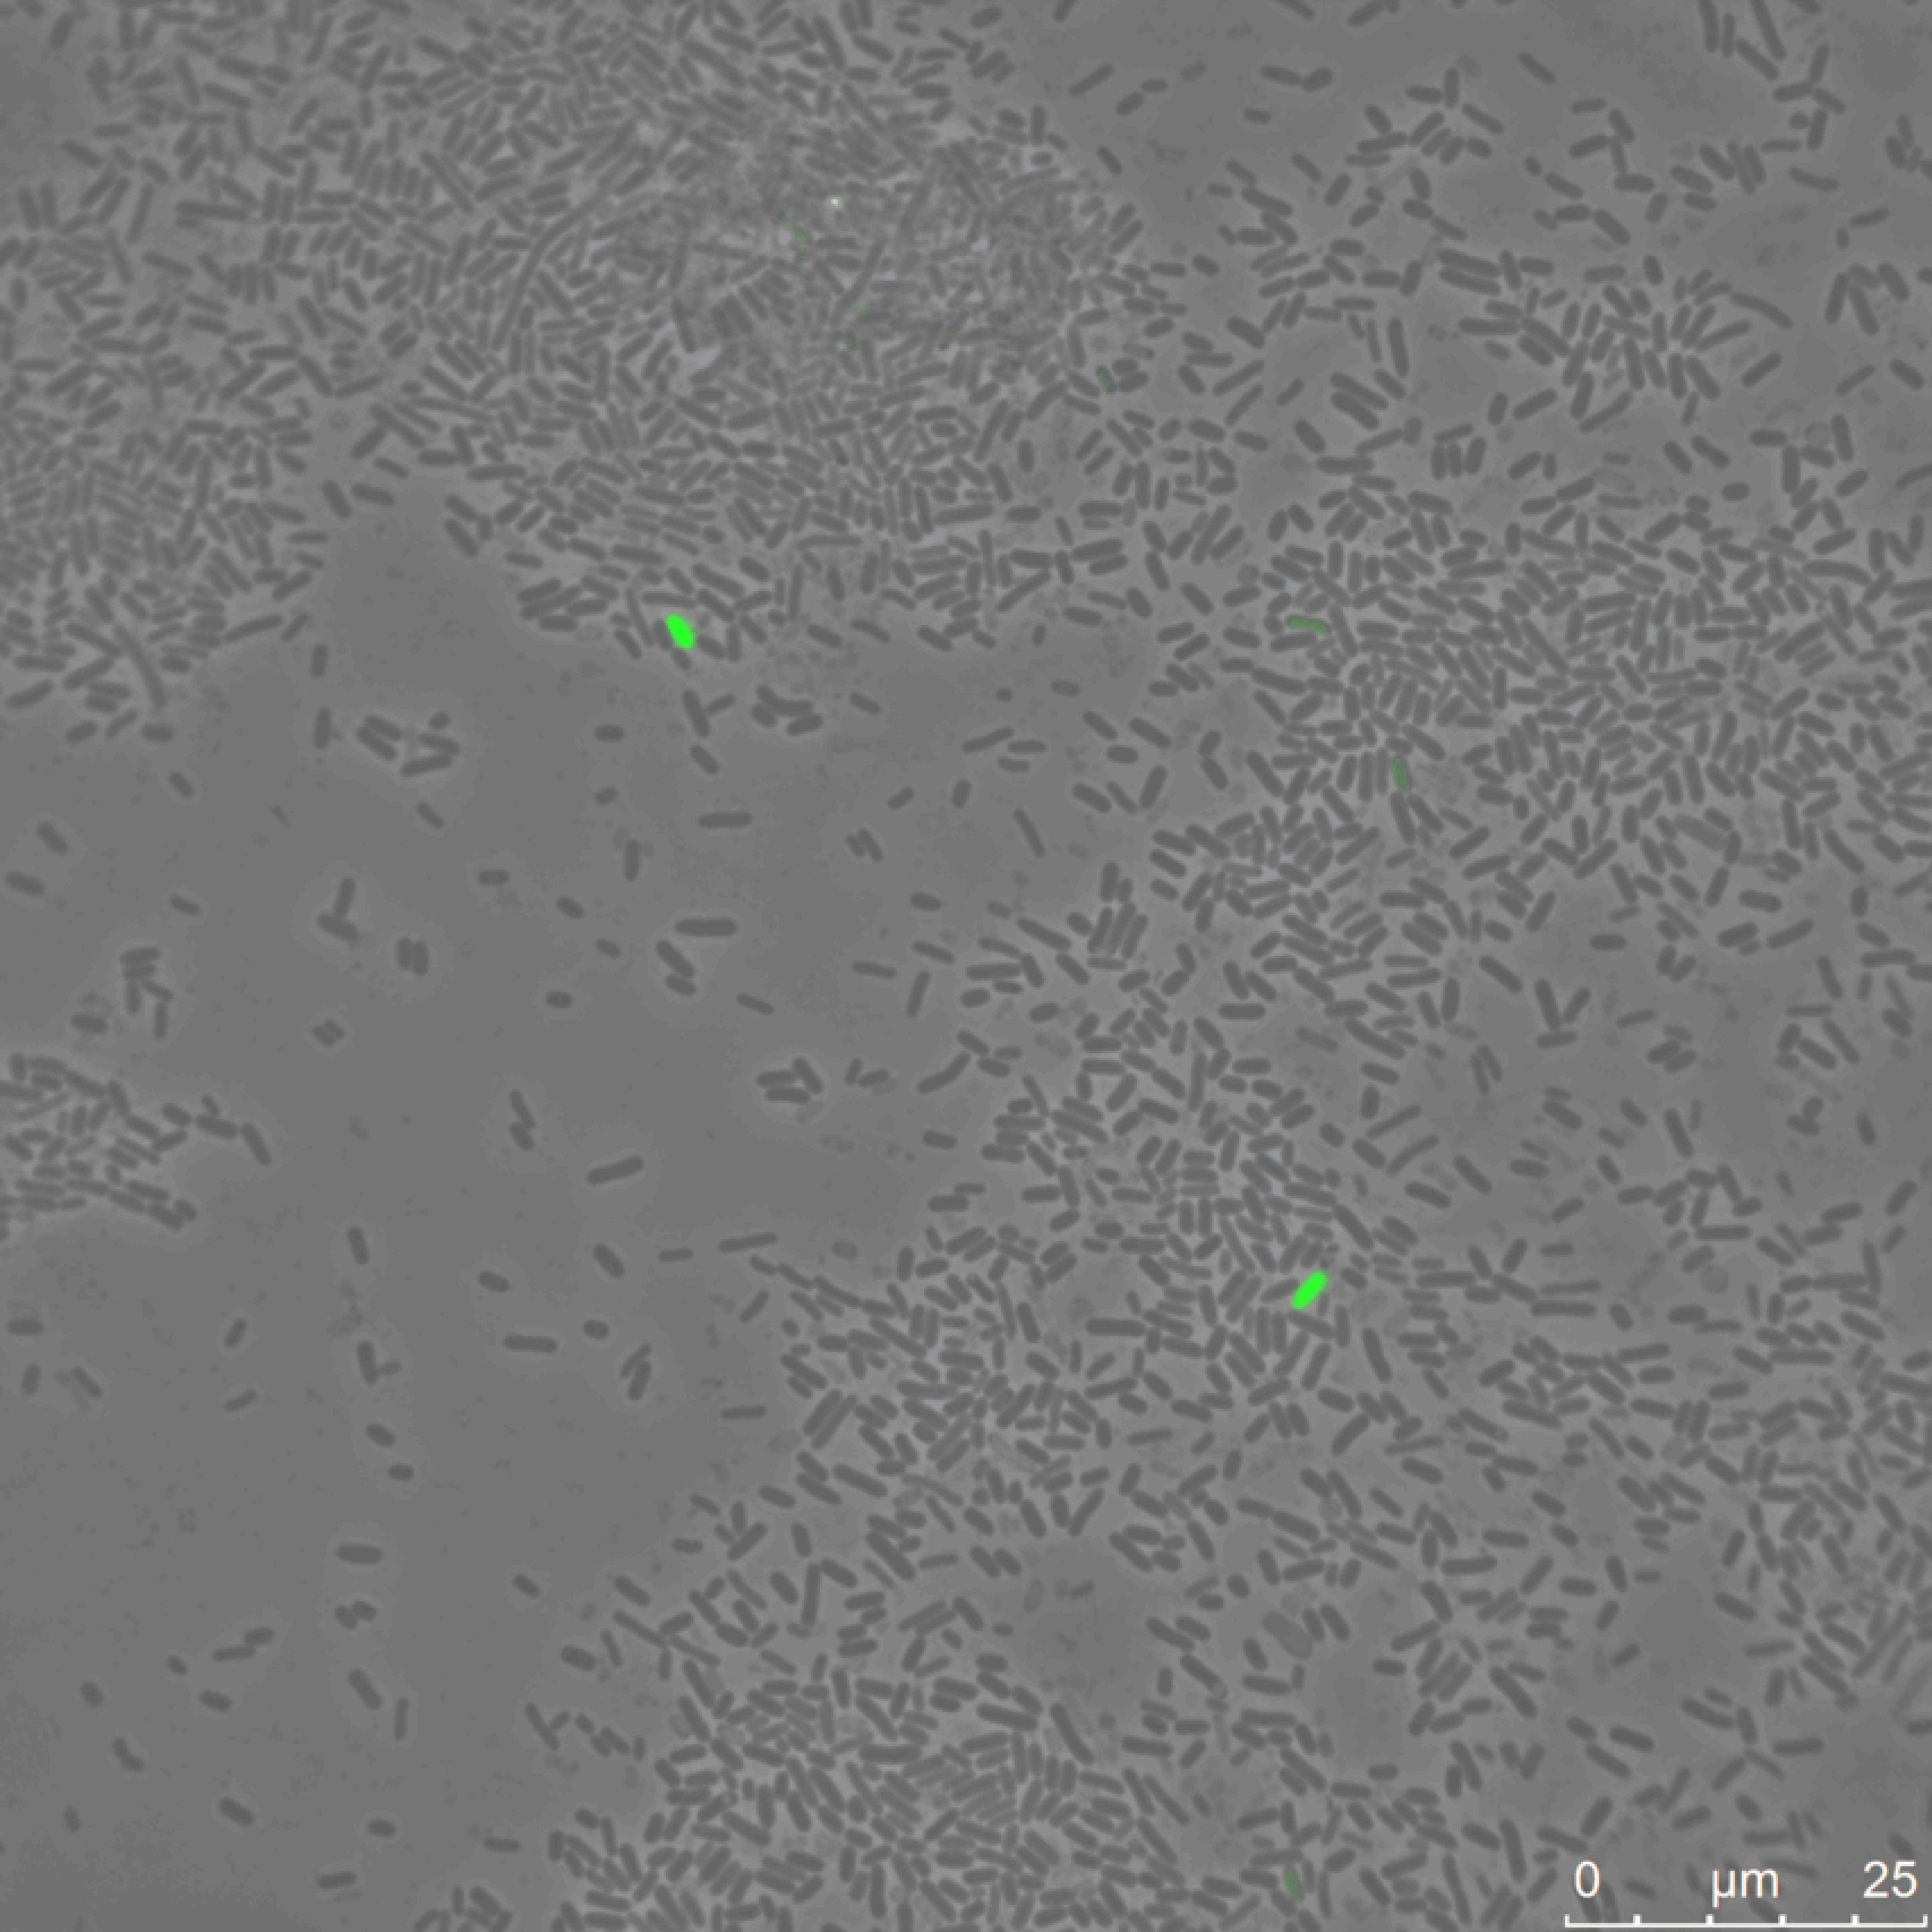
\includegraphics{THAIU1_24HR_6_GREEN-crunch-lighter-resample.pdf} &%
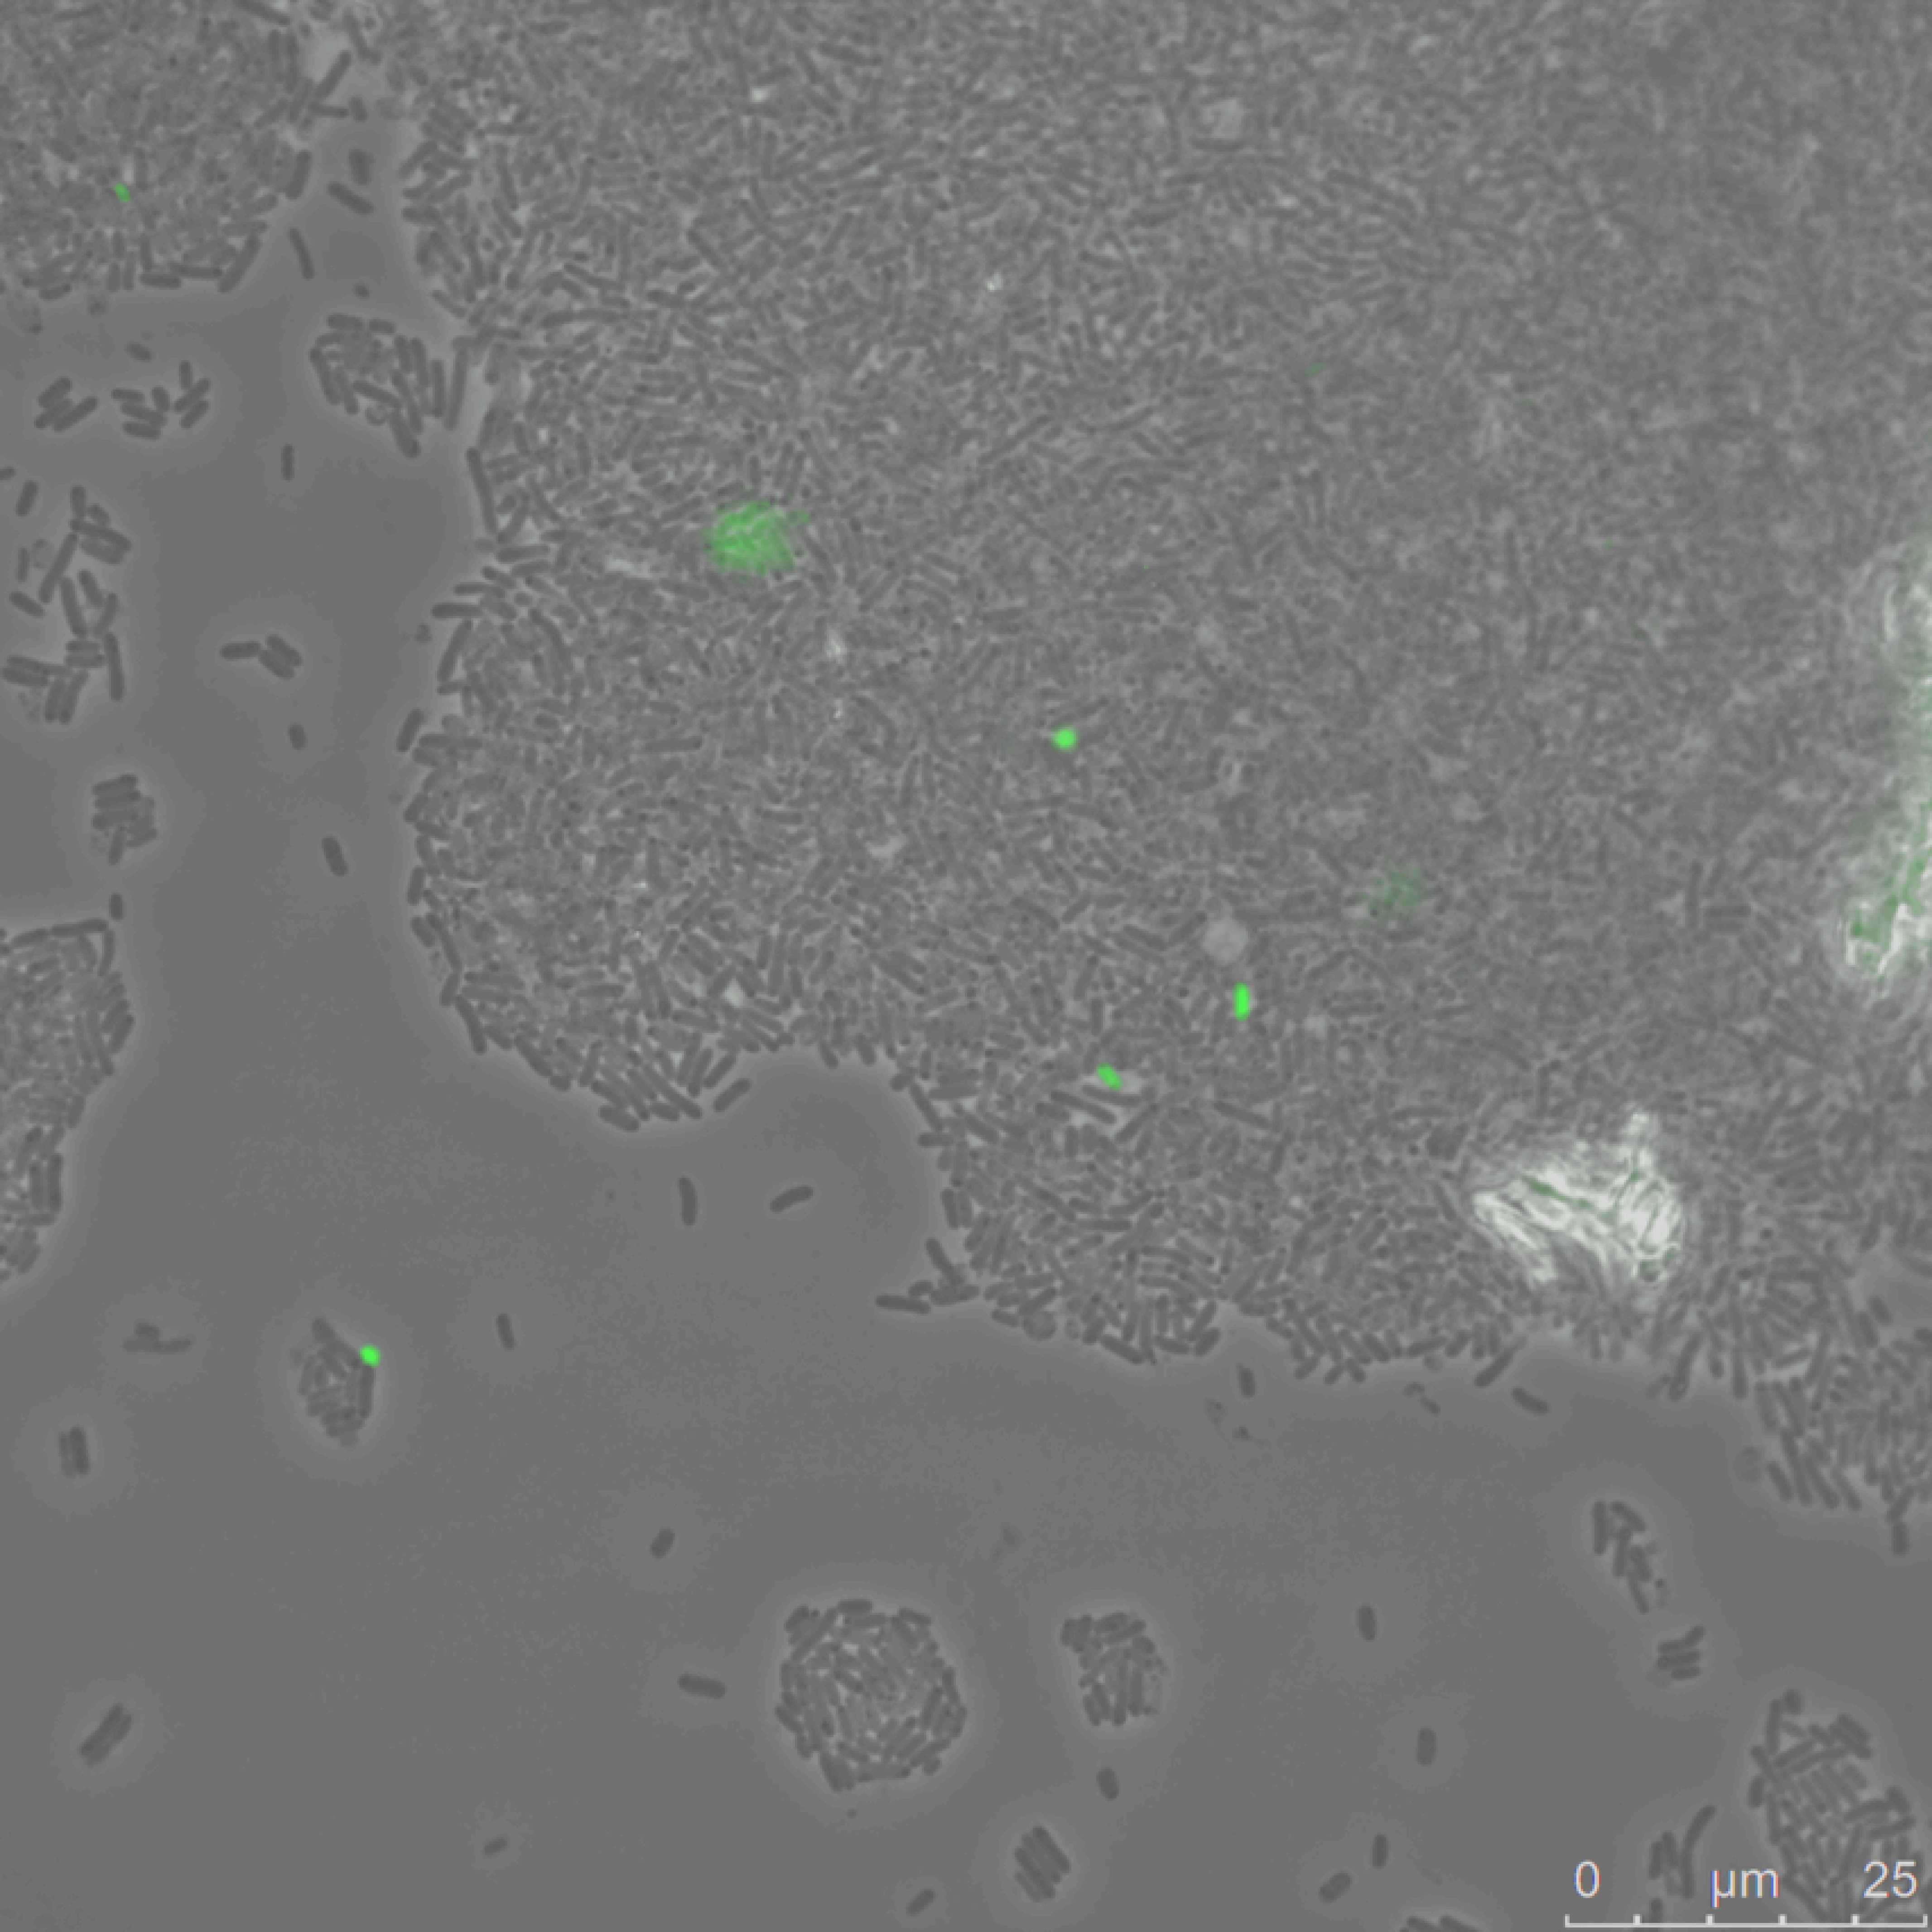
\includegraphics{THAIU1_72HR_3_GREEN-crunch-lighter-resample.pdf} \\[-0.5ex]

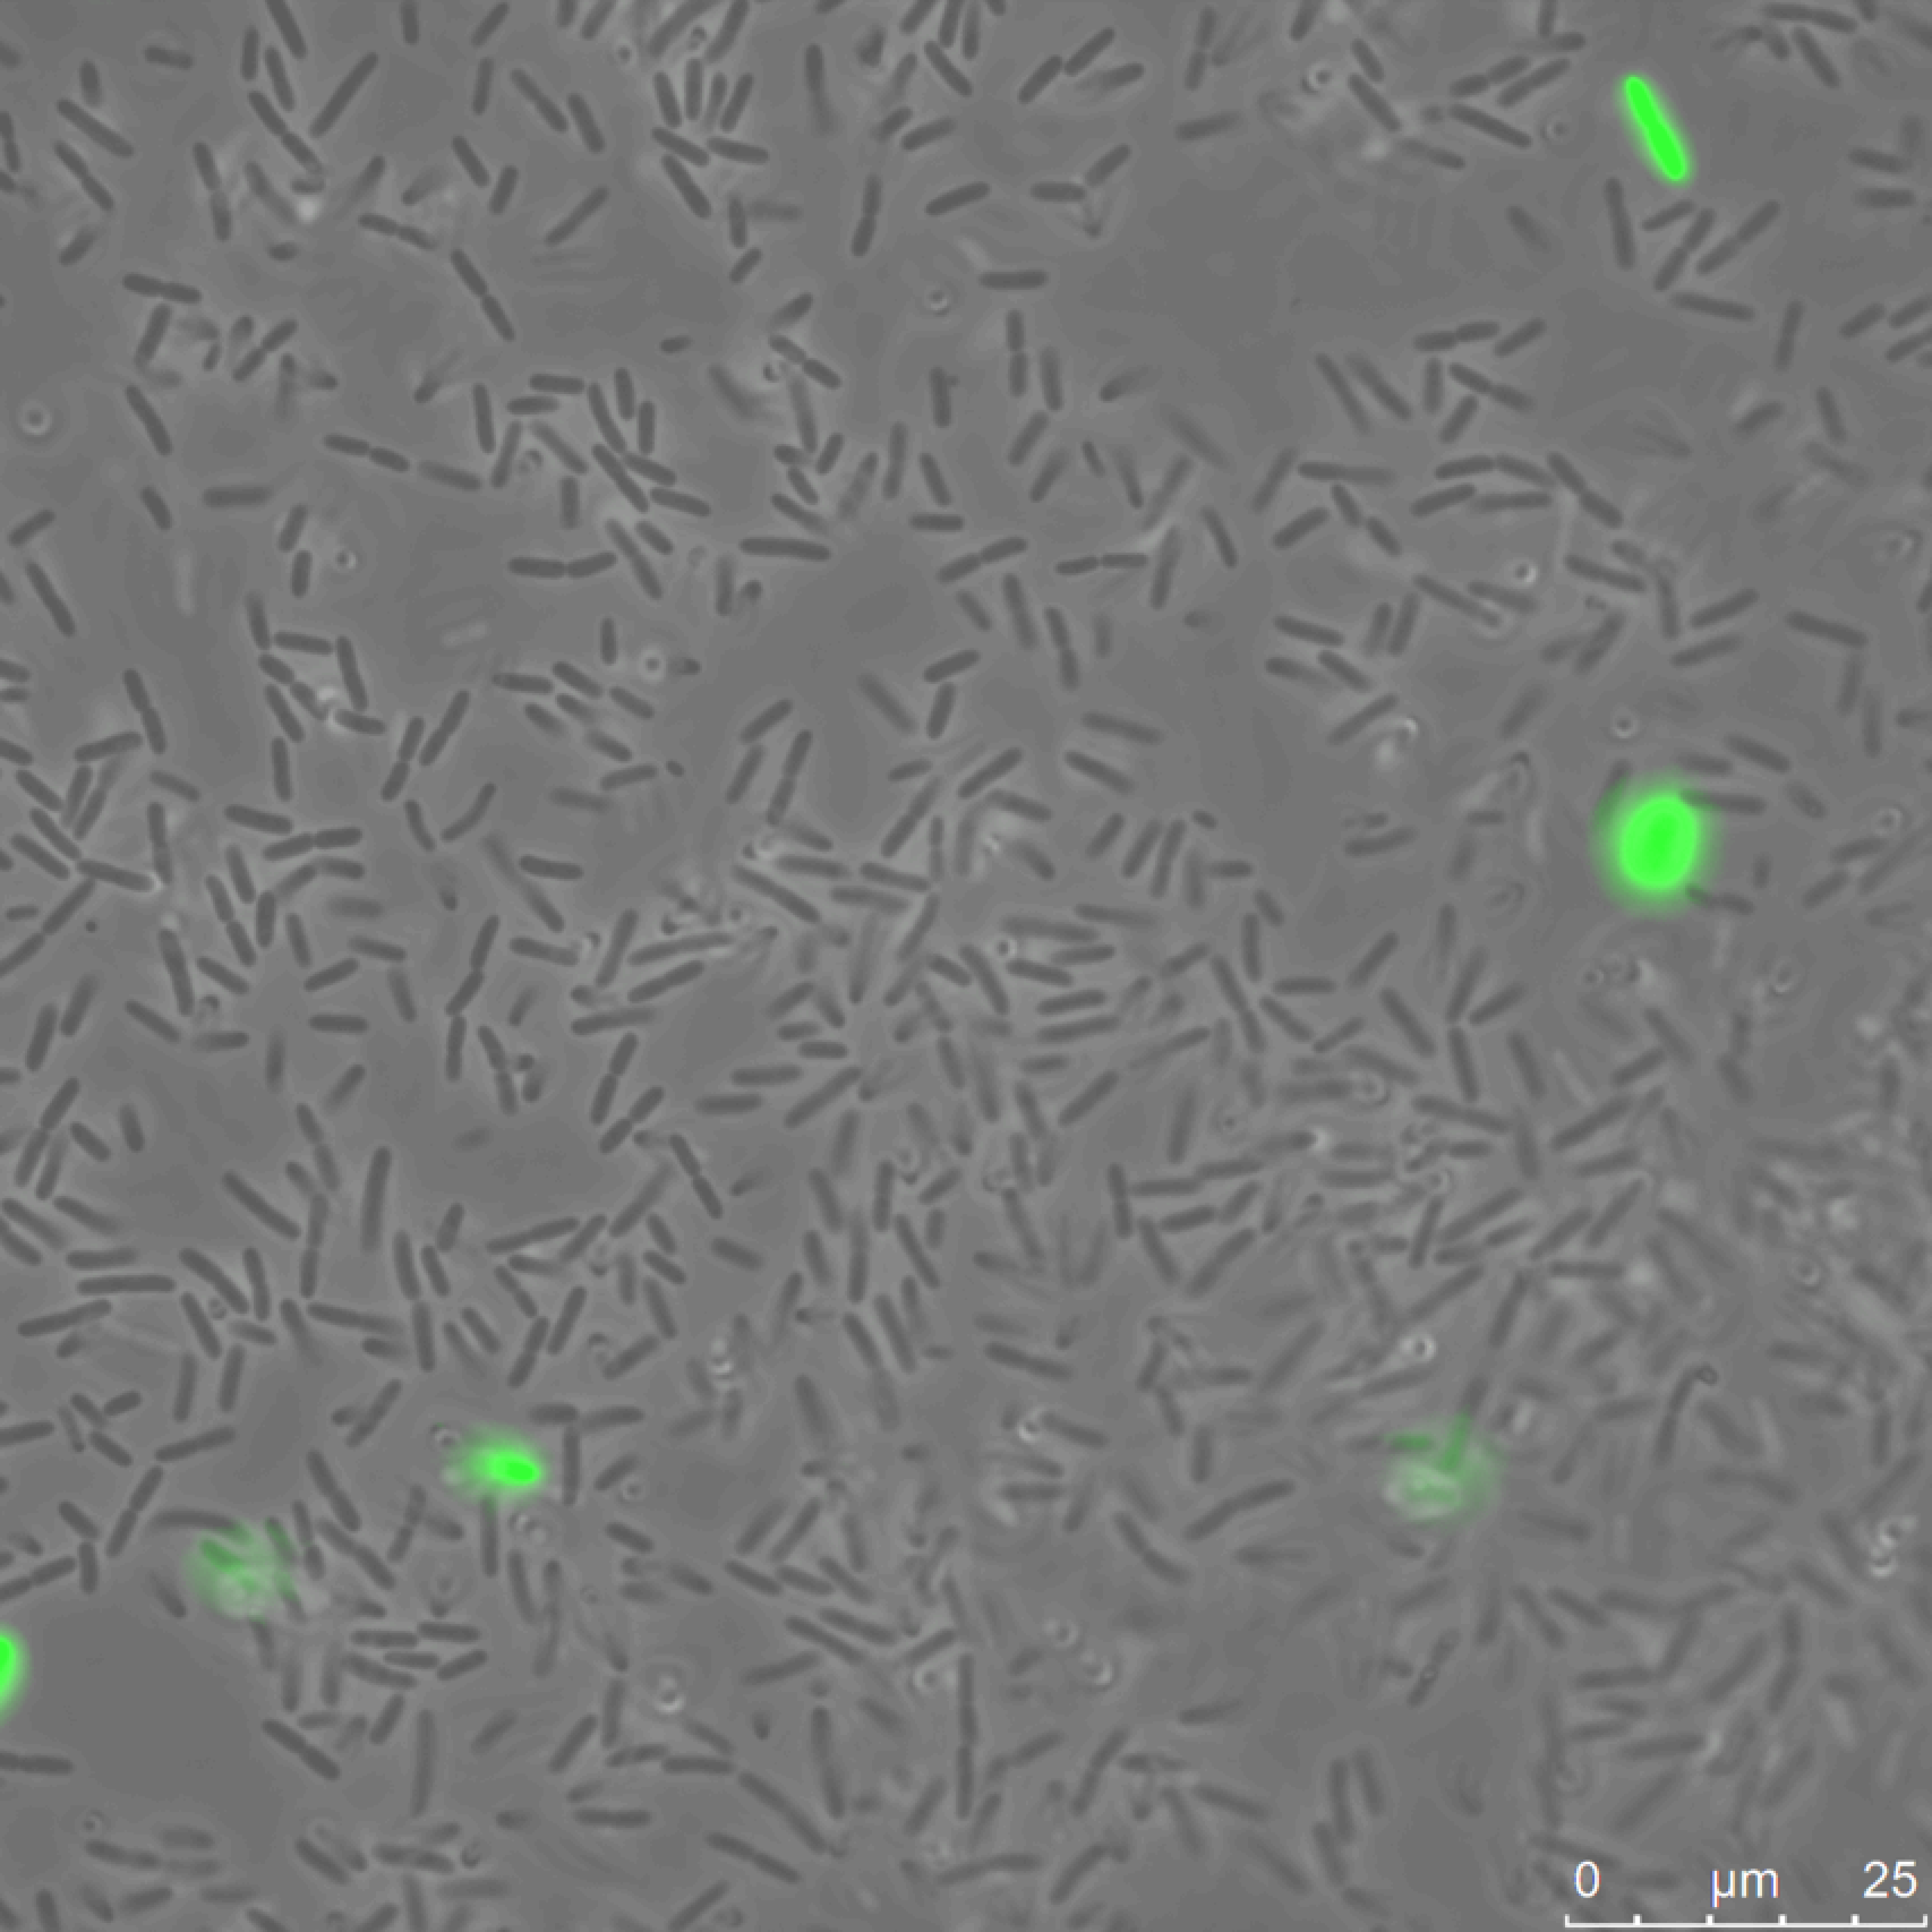
\includegraphics{THAIU1_4_GREEN-crunch-lighter-resample.pdf} &%
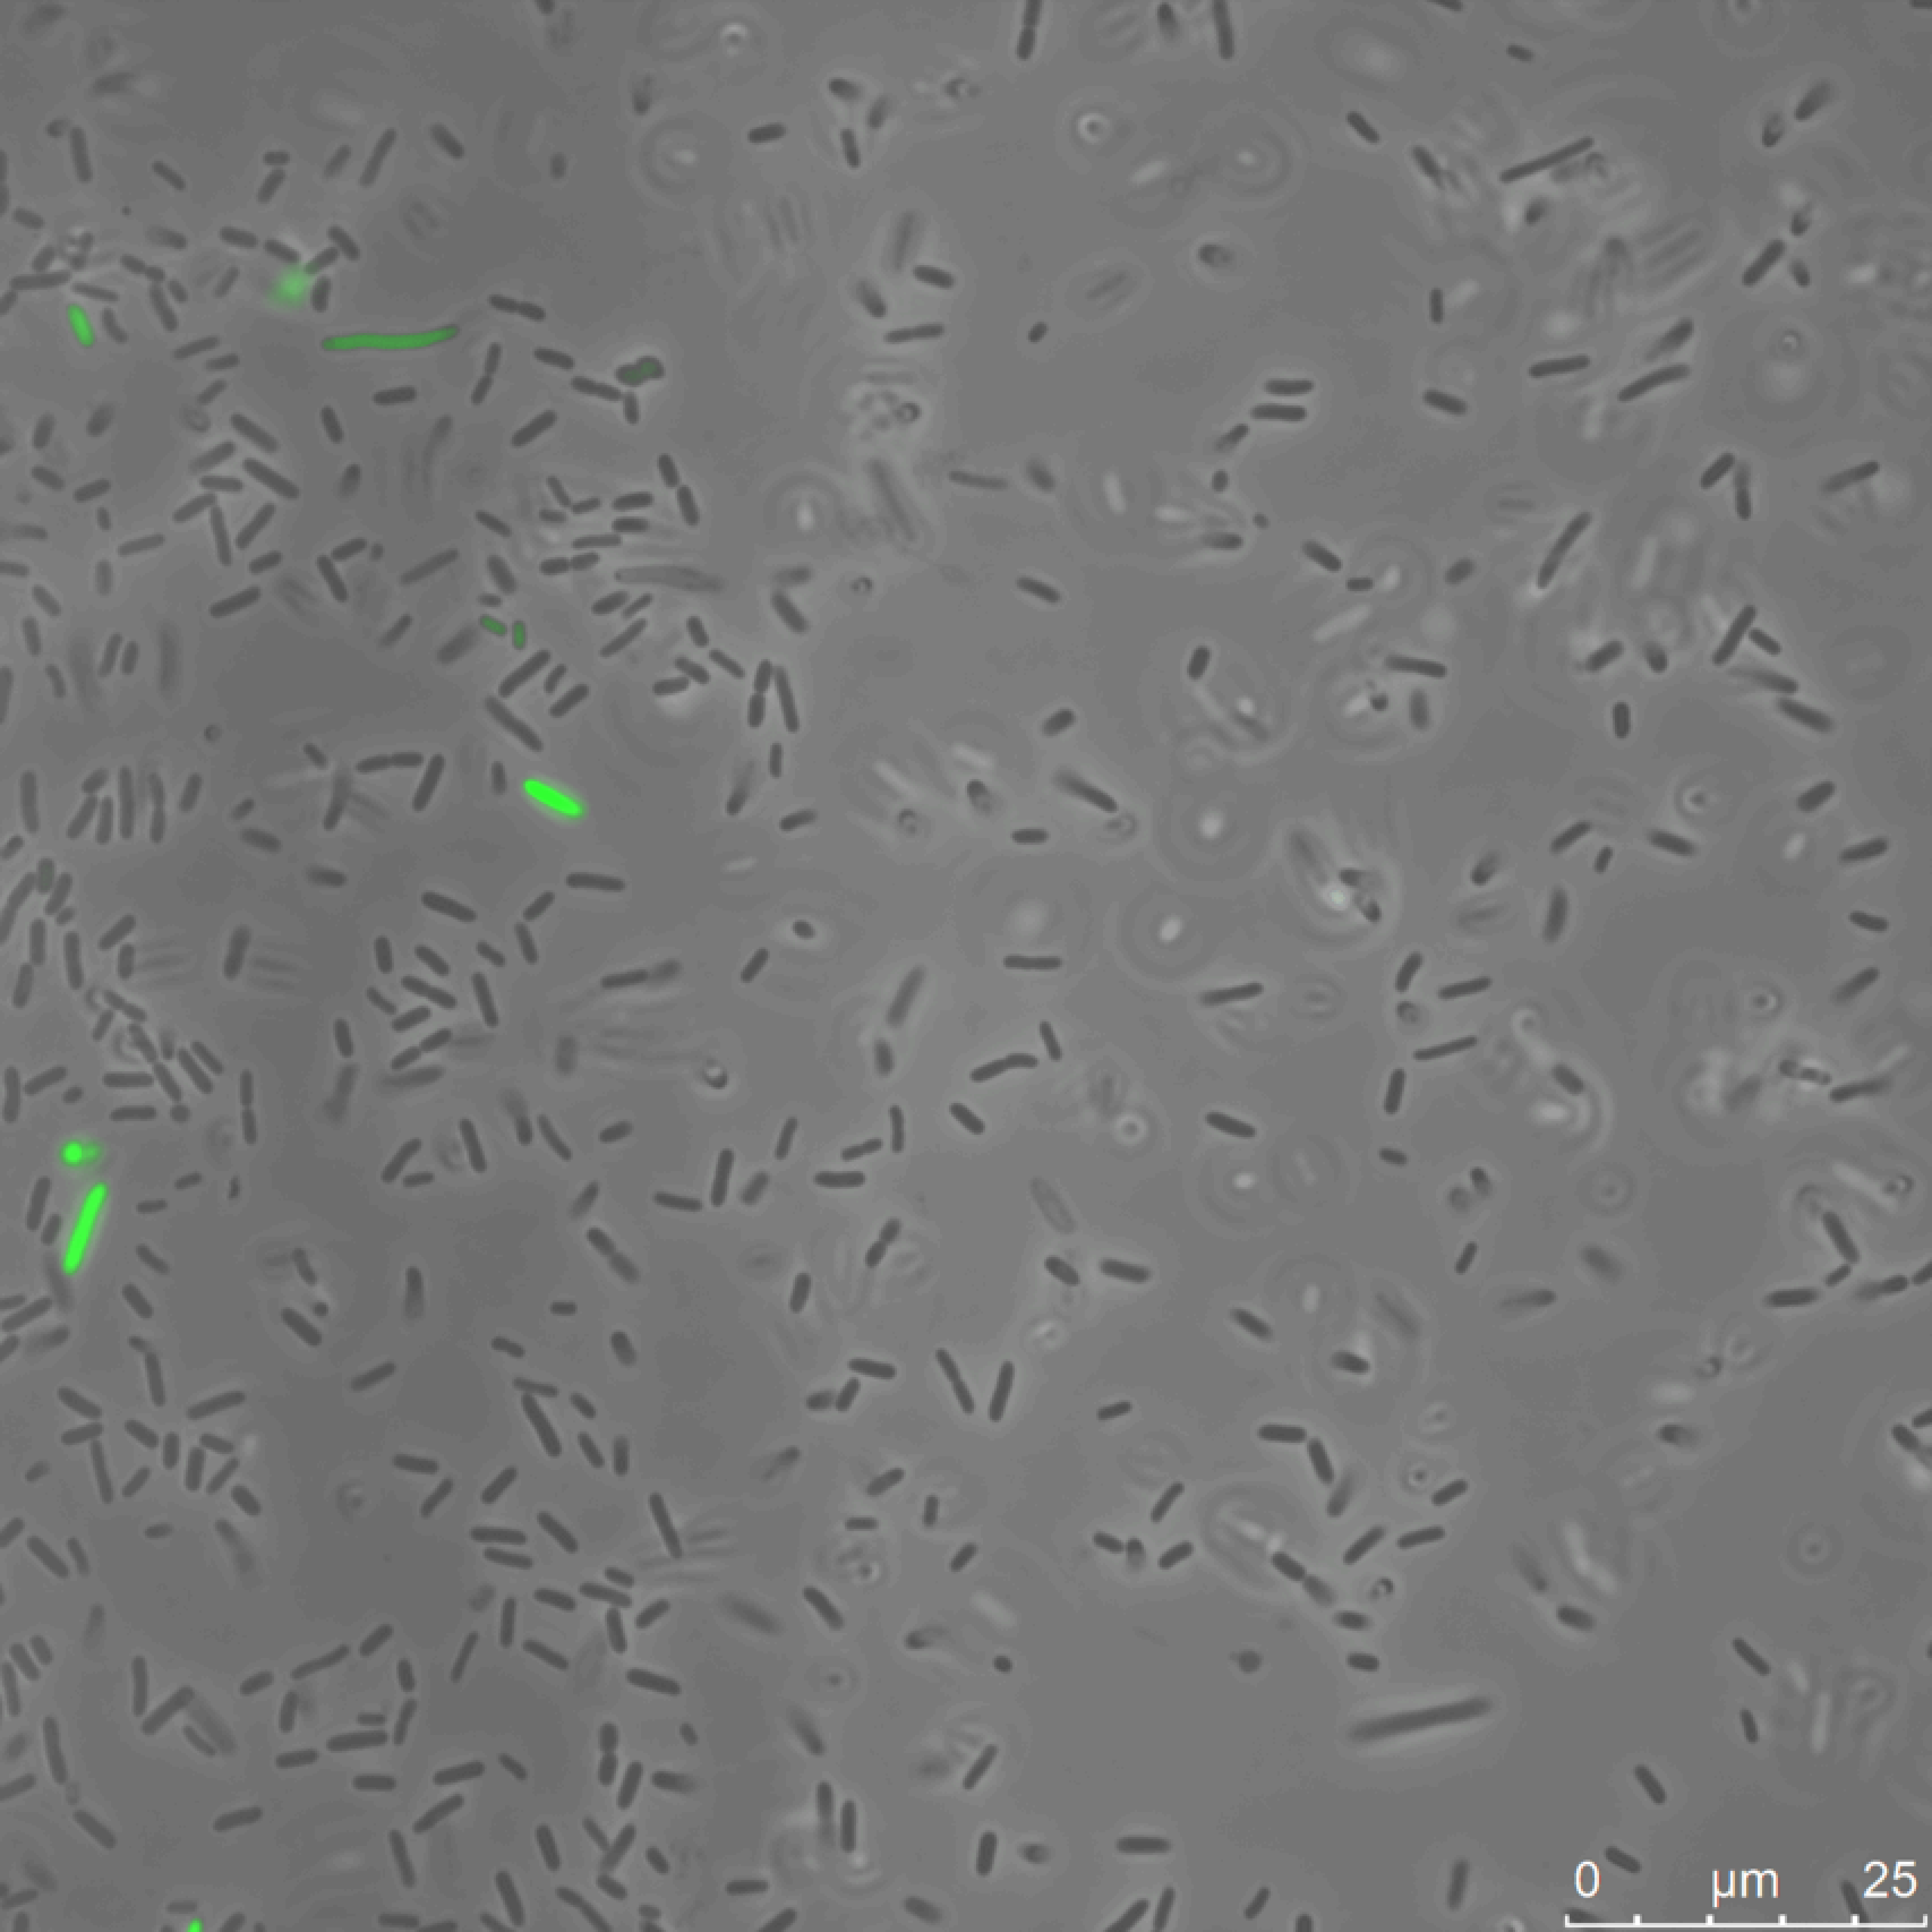
\includegraphics{THAIU1_5HR_6_GREEN-crunch-lighter-resample.pdf} &%
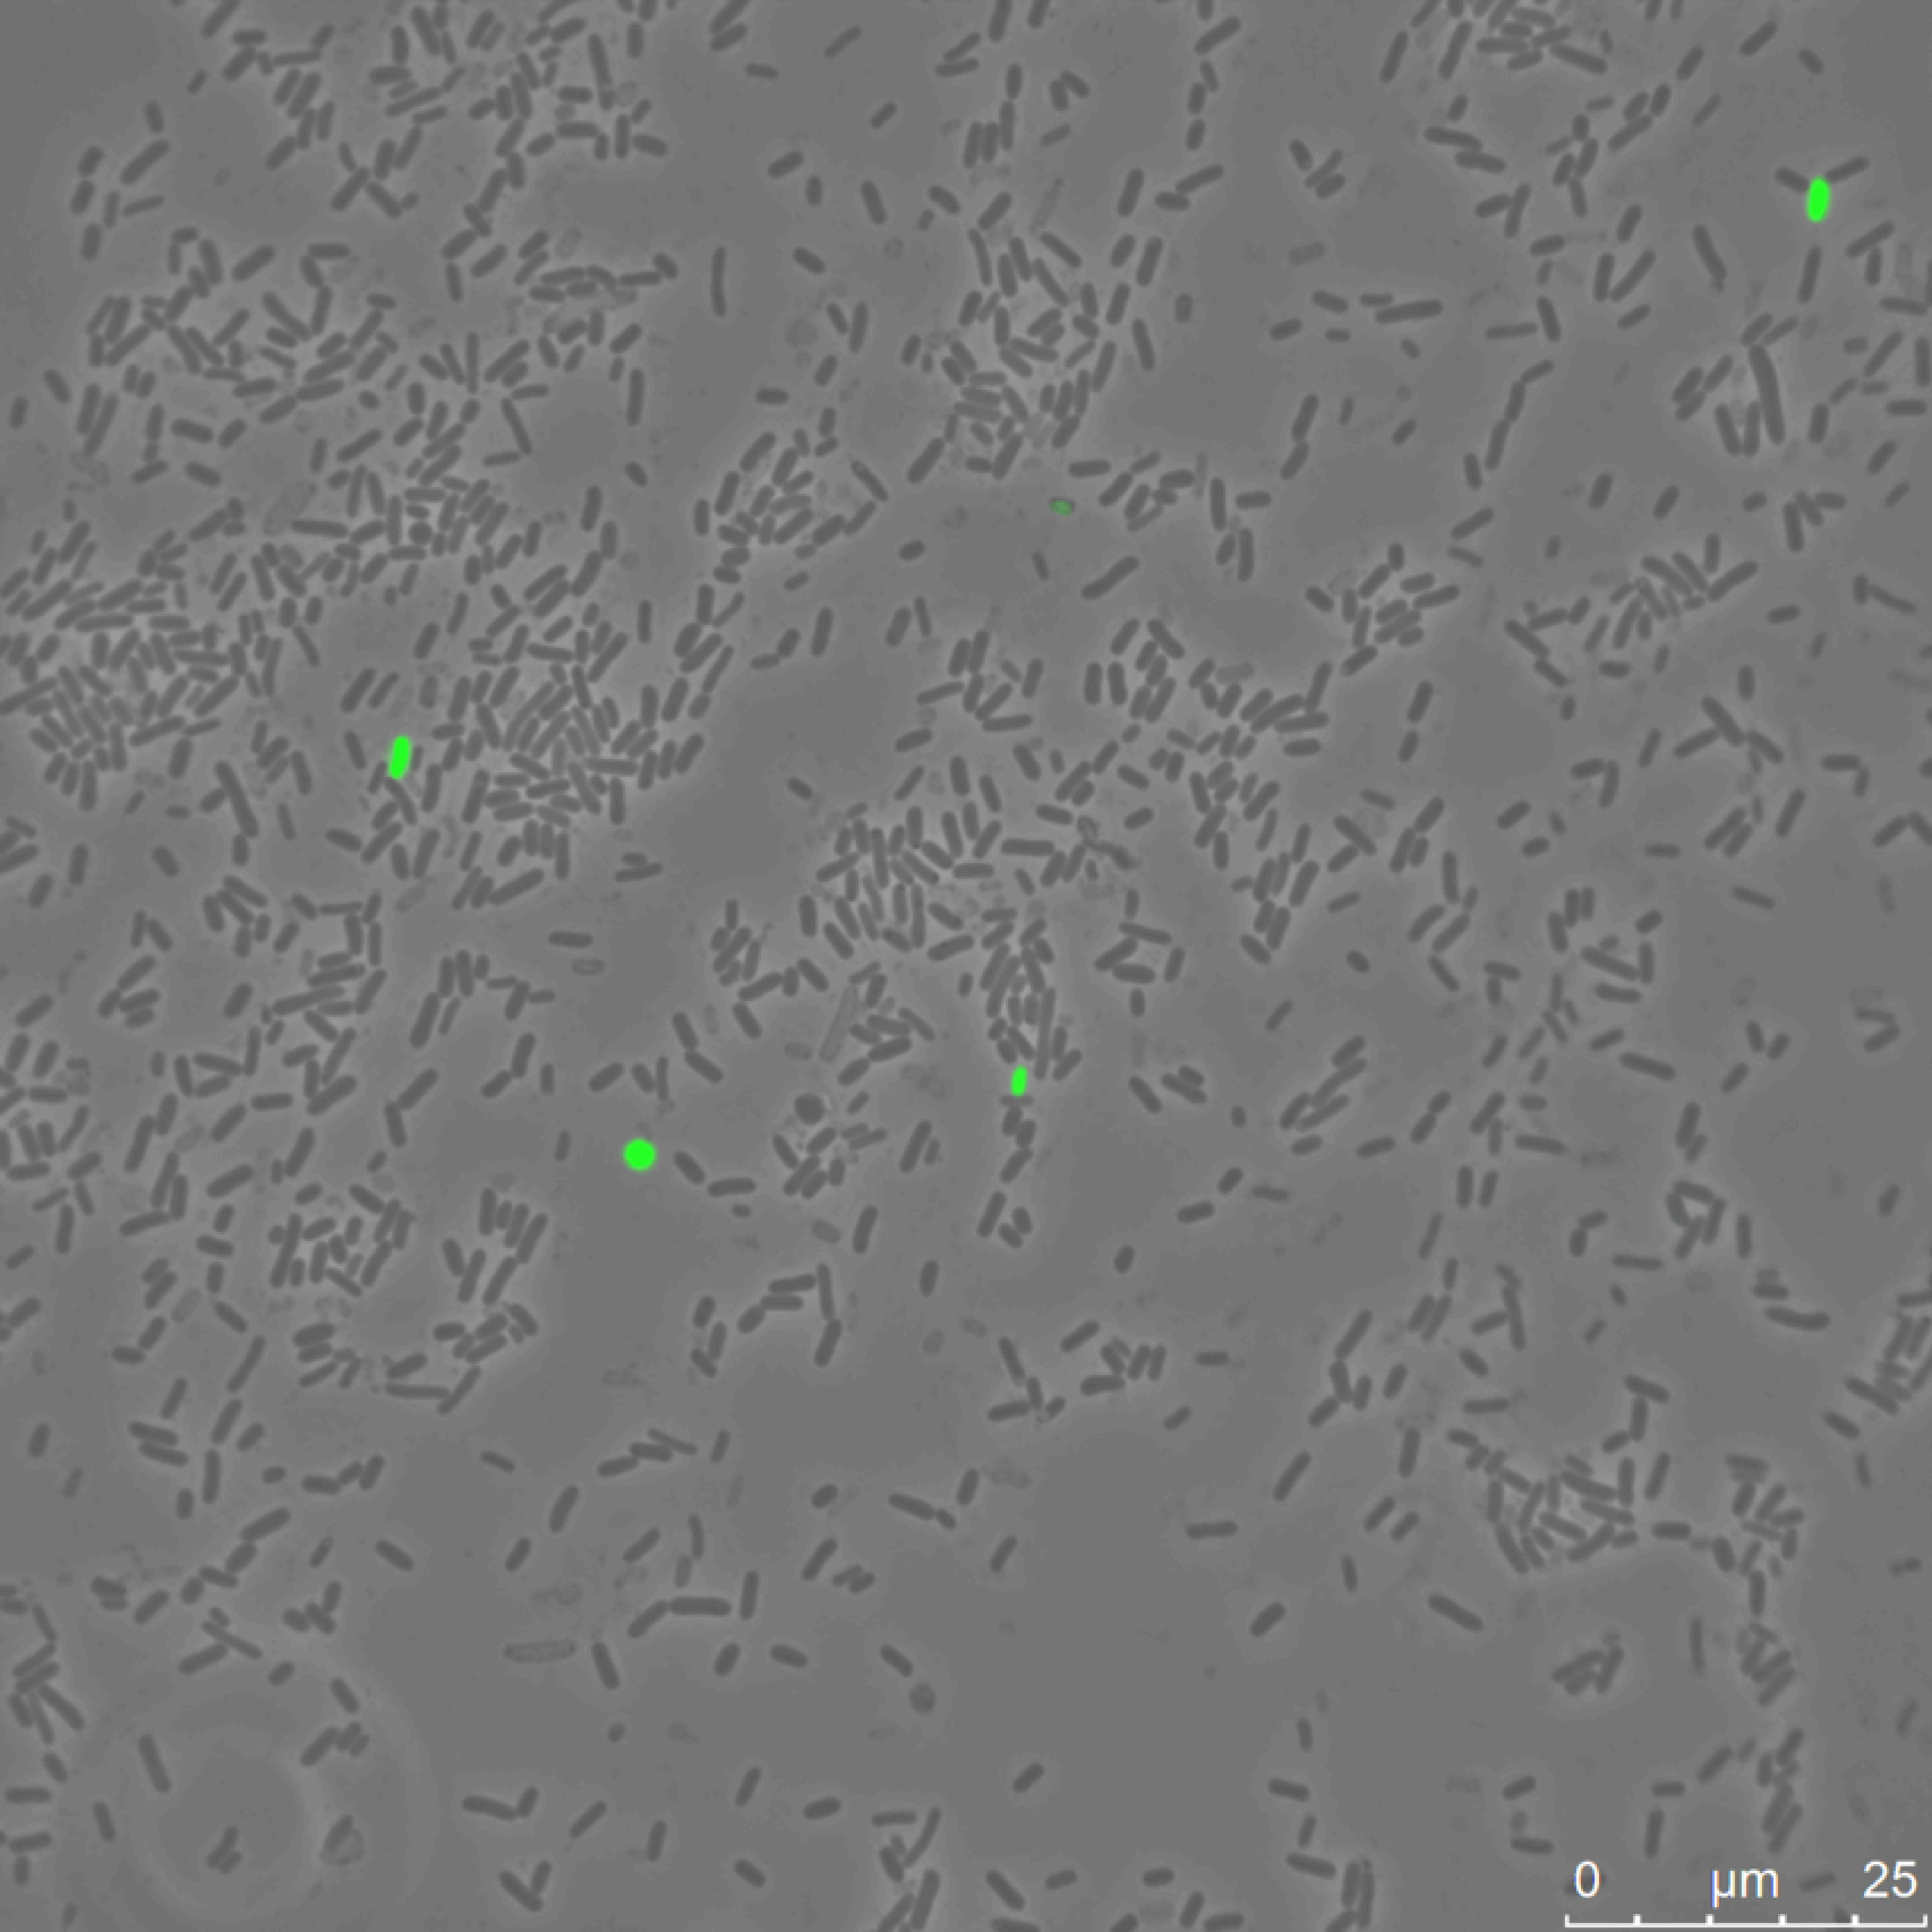
\includegraphics{THAIU1_24HR_8_GREEN-crunch-lighter-resample.pdf} &%
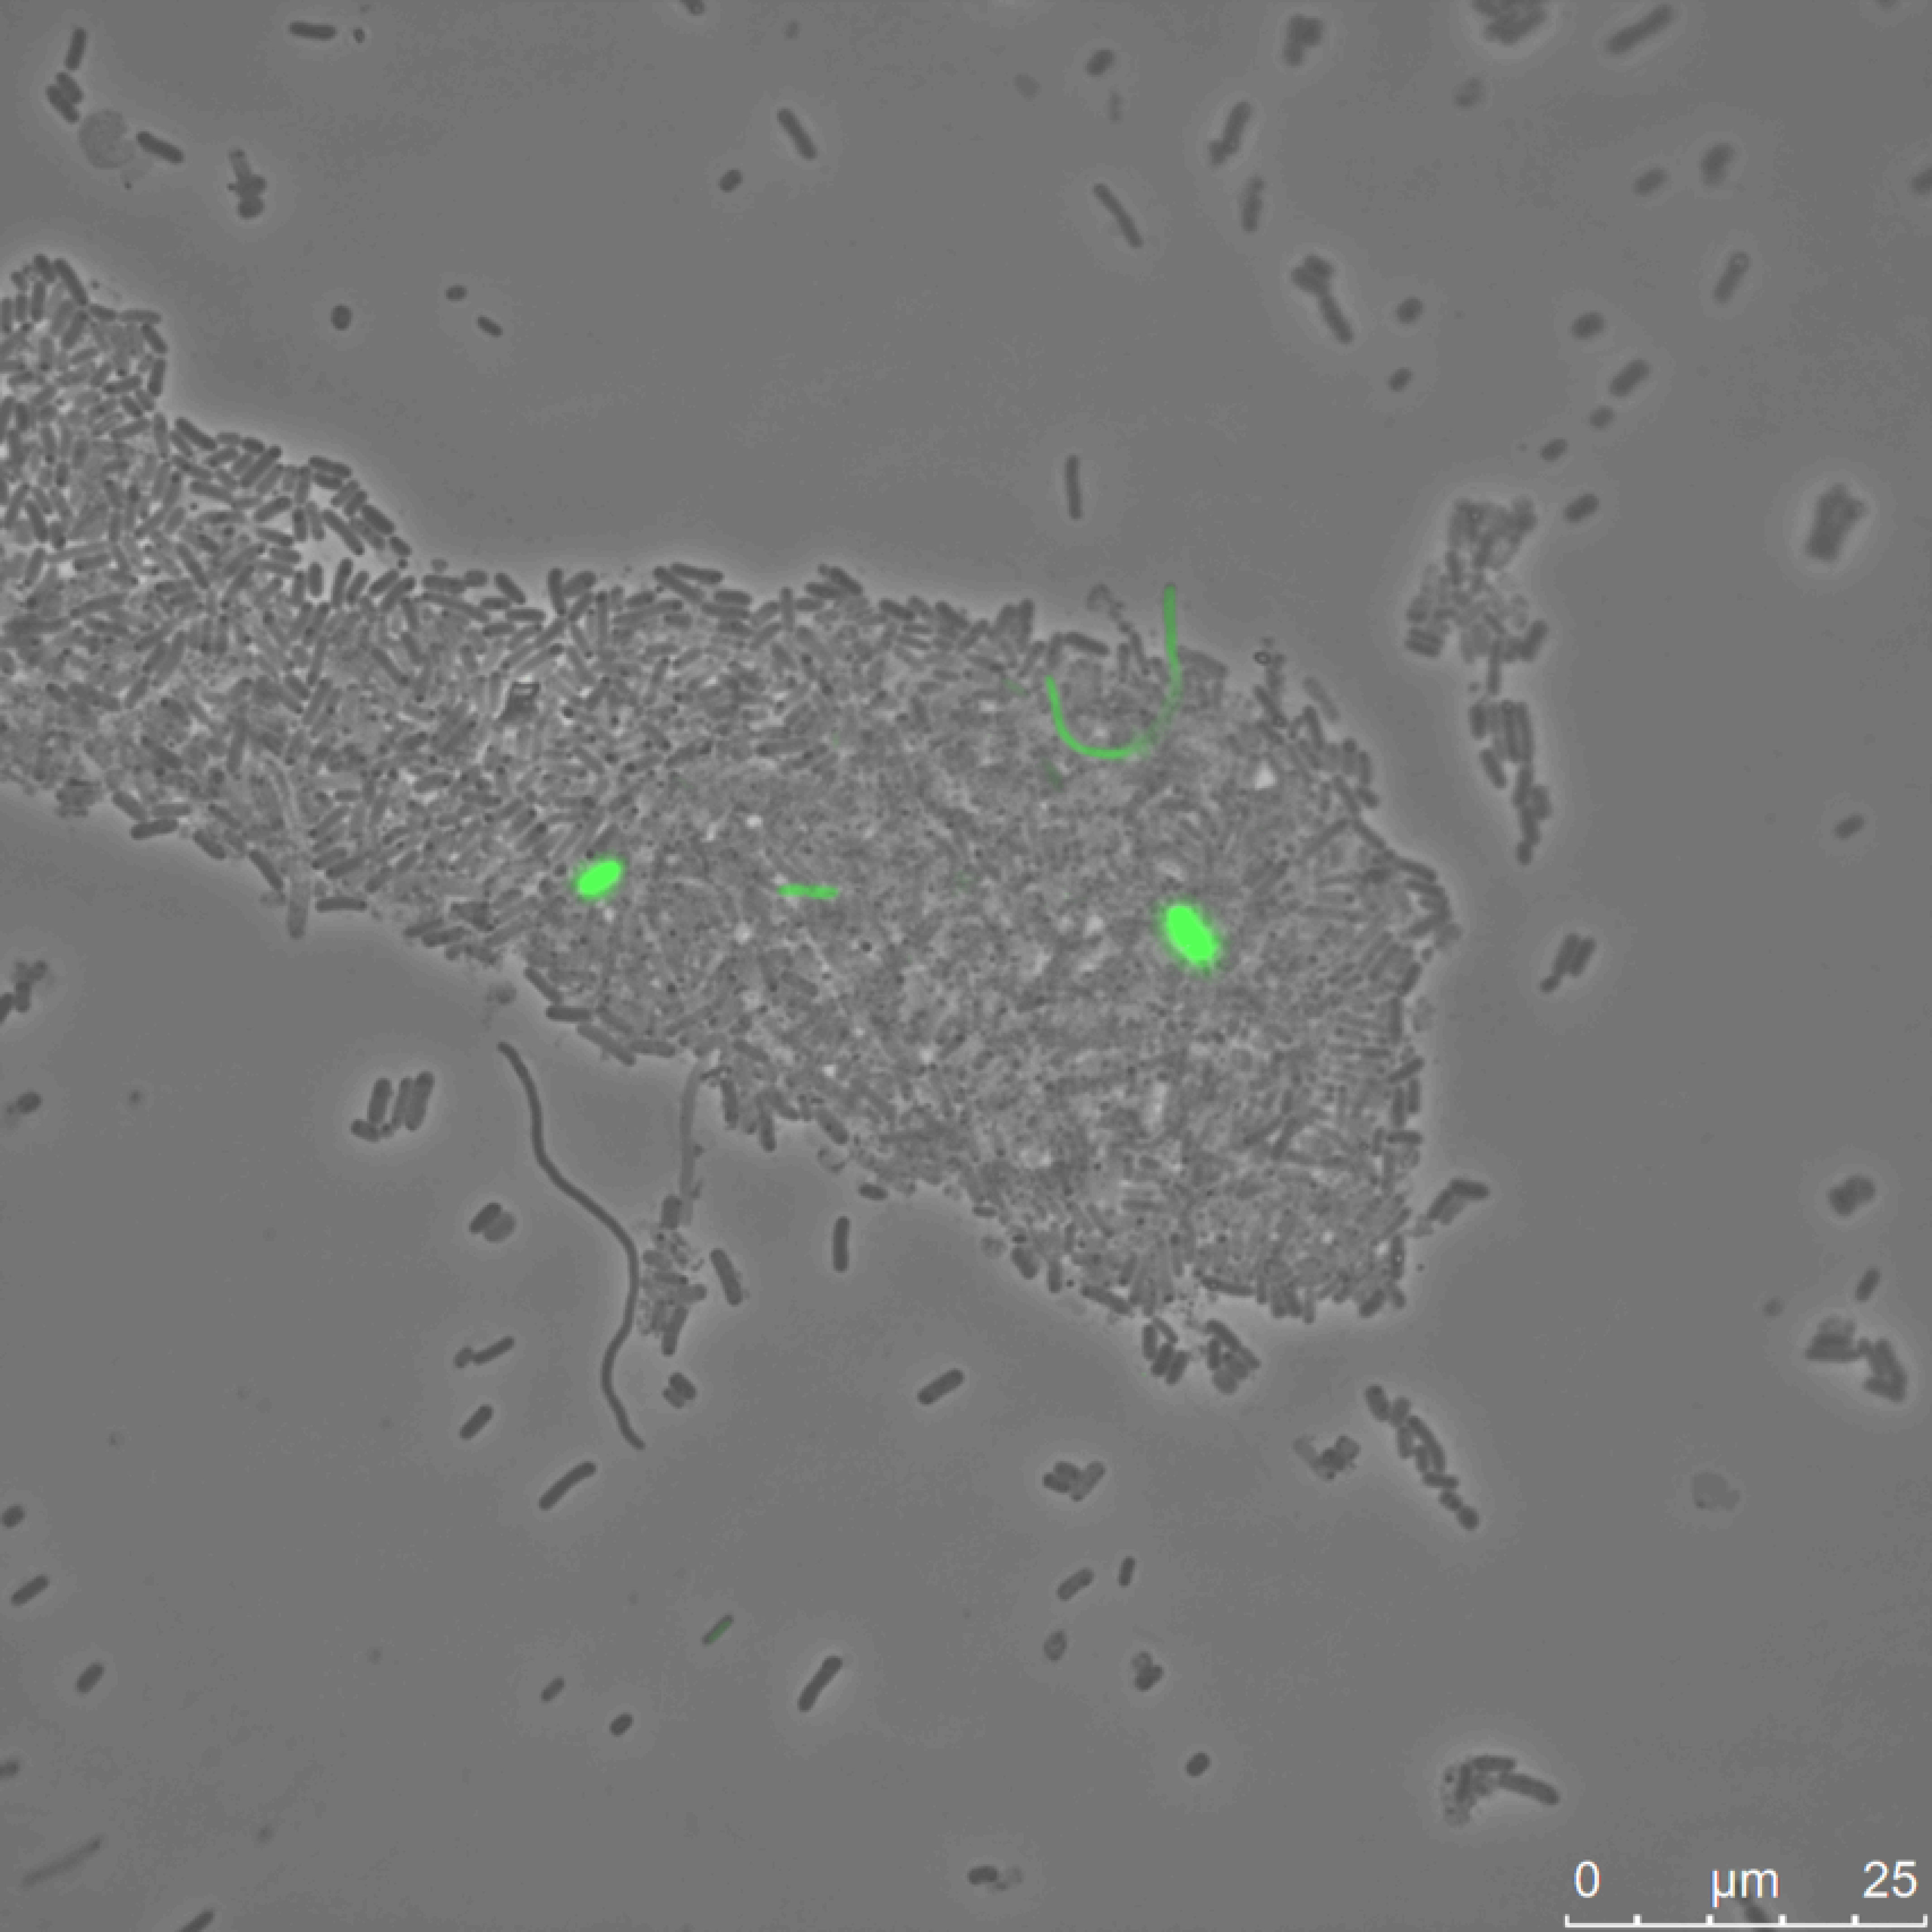
\includegraphics{THAIU1_72HR_4_GREEN-crunch-lighter-resample.pdf} \\
 ++ & ++ & ++ & ++ \\[1ex]

\end{tabularx}
\captionsetup{singlelinecheck=off, justification=justified, font=footnotesize, aboveskip=20pt}
\caption[Reporter microscopy - PB68.1 Unit 1]{\textsc{\normalsize Reporter microscopy for the \emph{P. asymbiotica} PB68.1 ``Unit 1" promoter.}\vspace{0.1cm} \newline A representative selection of images for 4 time points, for the PVC ``Unit 1" promoter fusion. Quadruplicate images are displayed vertically as representative of the whole slide sample. Key to qualitative fluorescence indication: ``-" - no fluorescence, ``+" - low level fluorescence in isolated cells. ``++" - low level fluorescence in many cells or few brighter cells, ``+++" - intermediate to high fluorescence in almost all cells, or very bright isolated cells.}
\end{figure}\label{RMTHAIU1}
\endgroup

%%%%%%%%%%%%%%%%%%%%%%%%%%%%%%%%%%%%%%%%%%%%%%%%%%%%%%%%%%%%%%%%%%%%

\begingroup
\renewcommand{\arraystretch}{0.8}%
\setlength{\tabcolsep}{0.3pt}
\begin{figure}[p]
\setkeys{Gin}{width=\linewidth}
\Huge
\begin{tabularx}{\textwidth}{CCCC}
\multicolumn{4}{p{\linewidth}}{\large \centering \textbf{\emph{P. luminescens} TT01 PVC ``Unit 4"}} \\
\hiderowcolors
& & & \\[-1.5ex]
\Large 2 Hours &\Large 5 Hours &\Large 24 Hours &\Large 72 Hours \\[1ex]

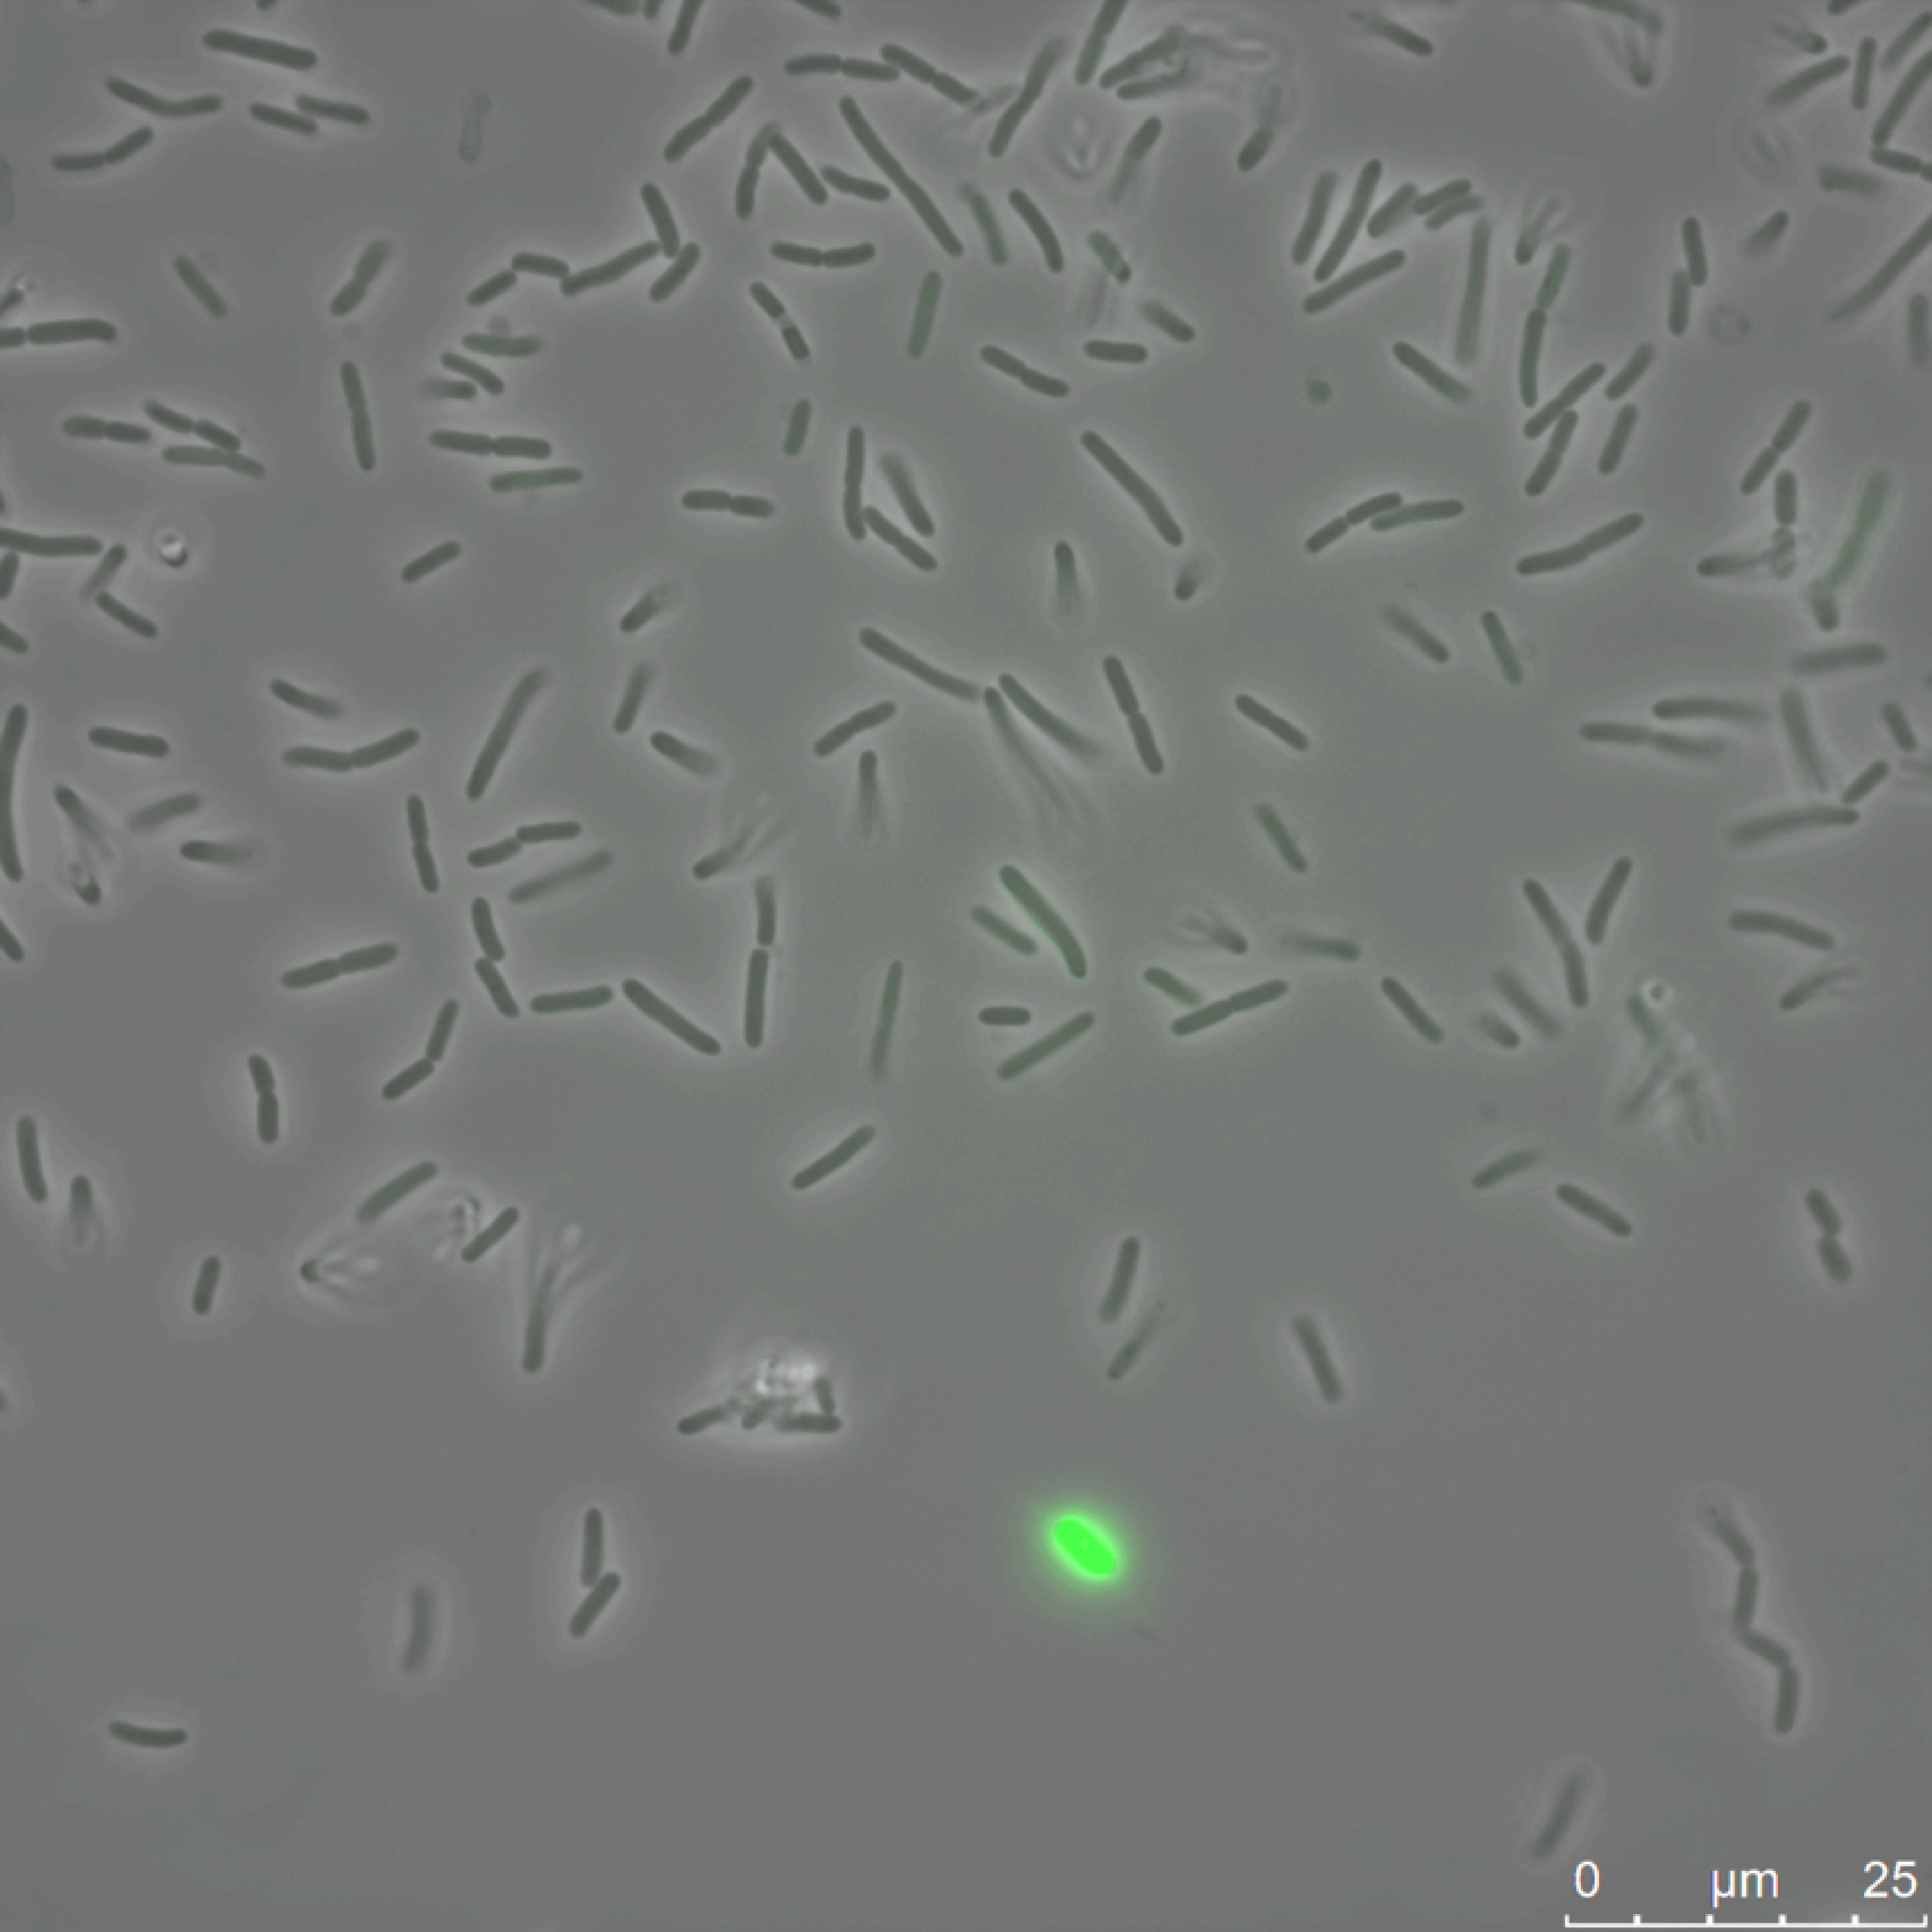
\includegraphics{TT01U4_1_GREEN-crunch-lighter-resample.pdf} &%
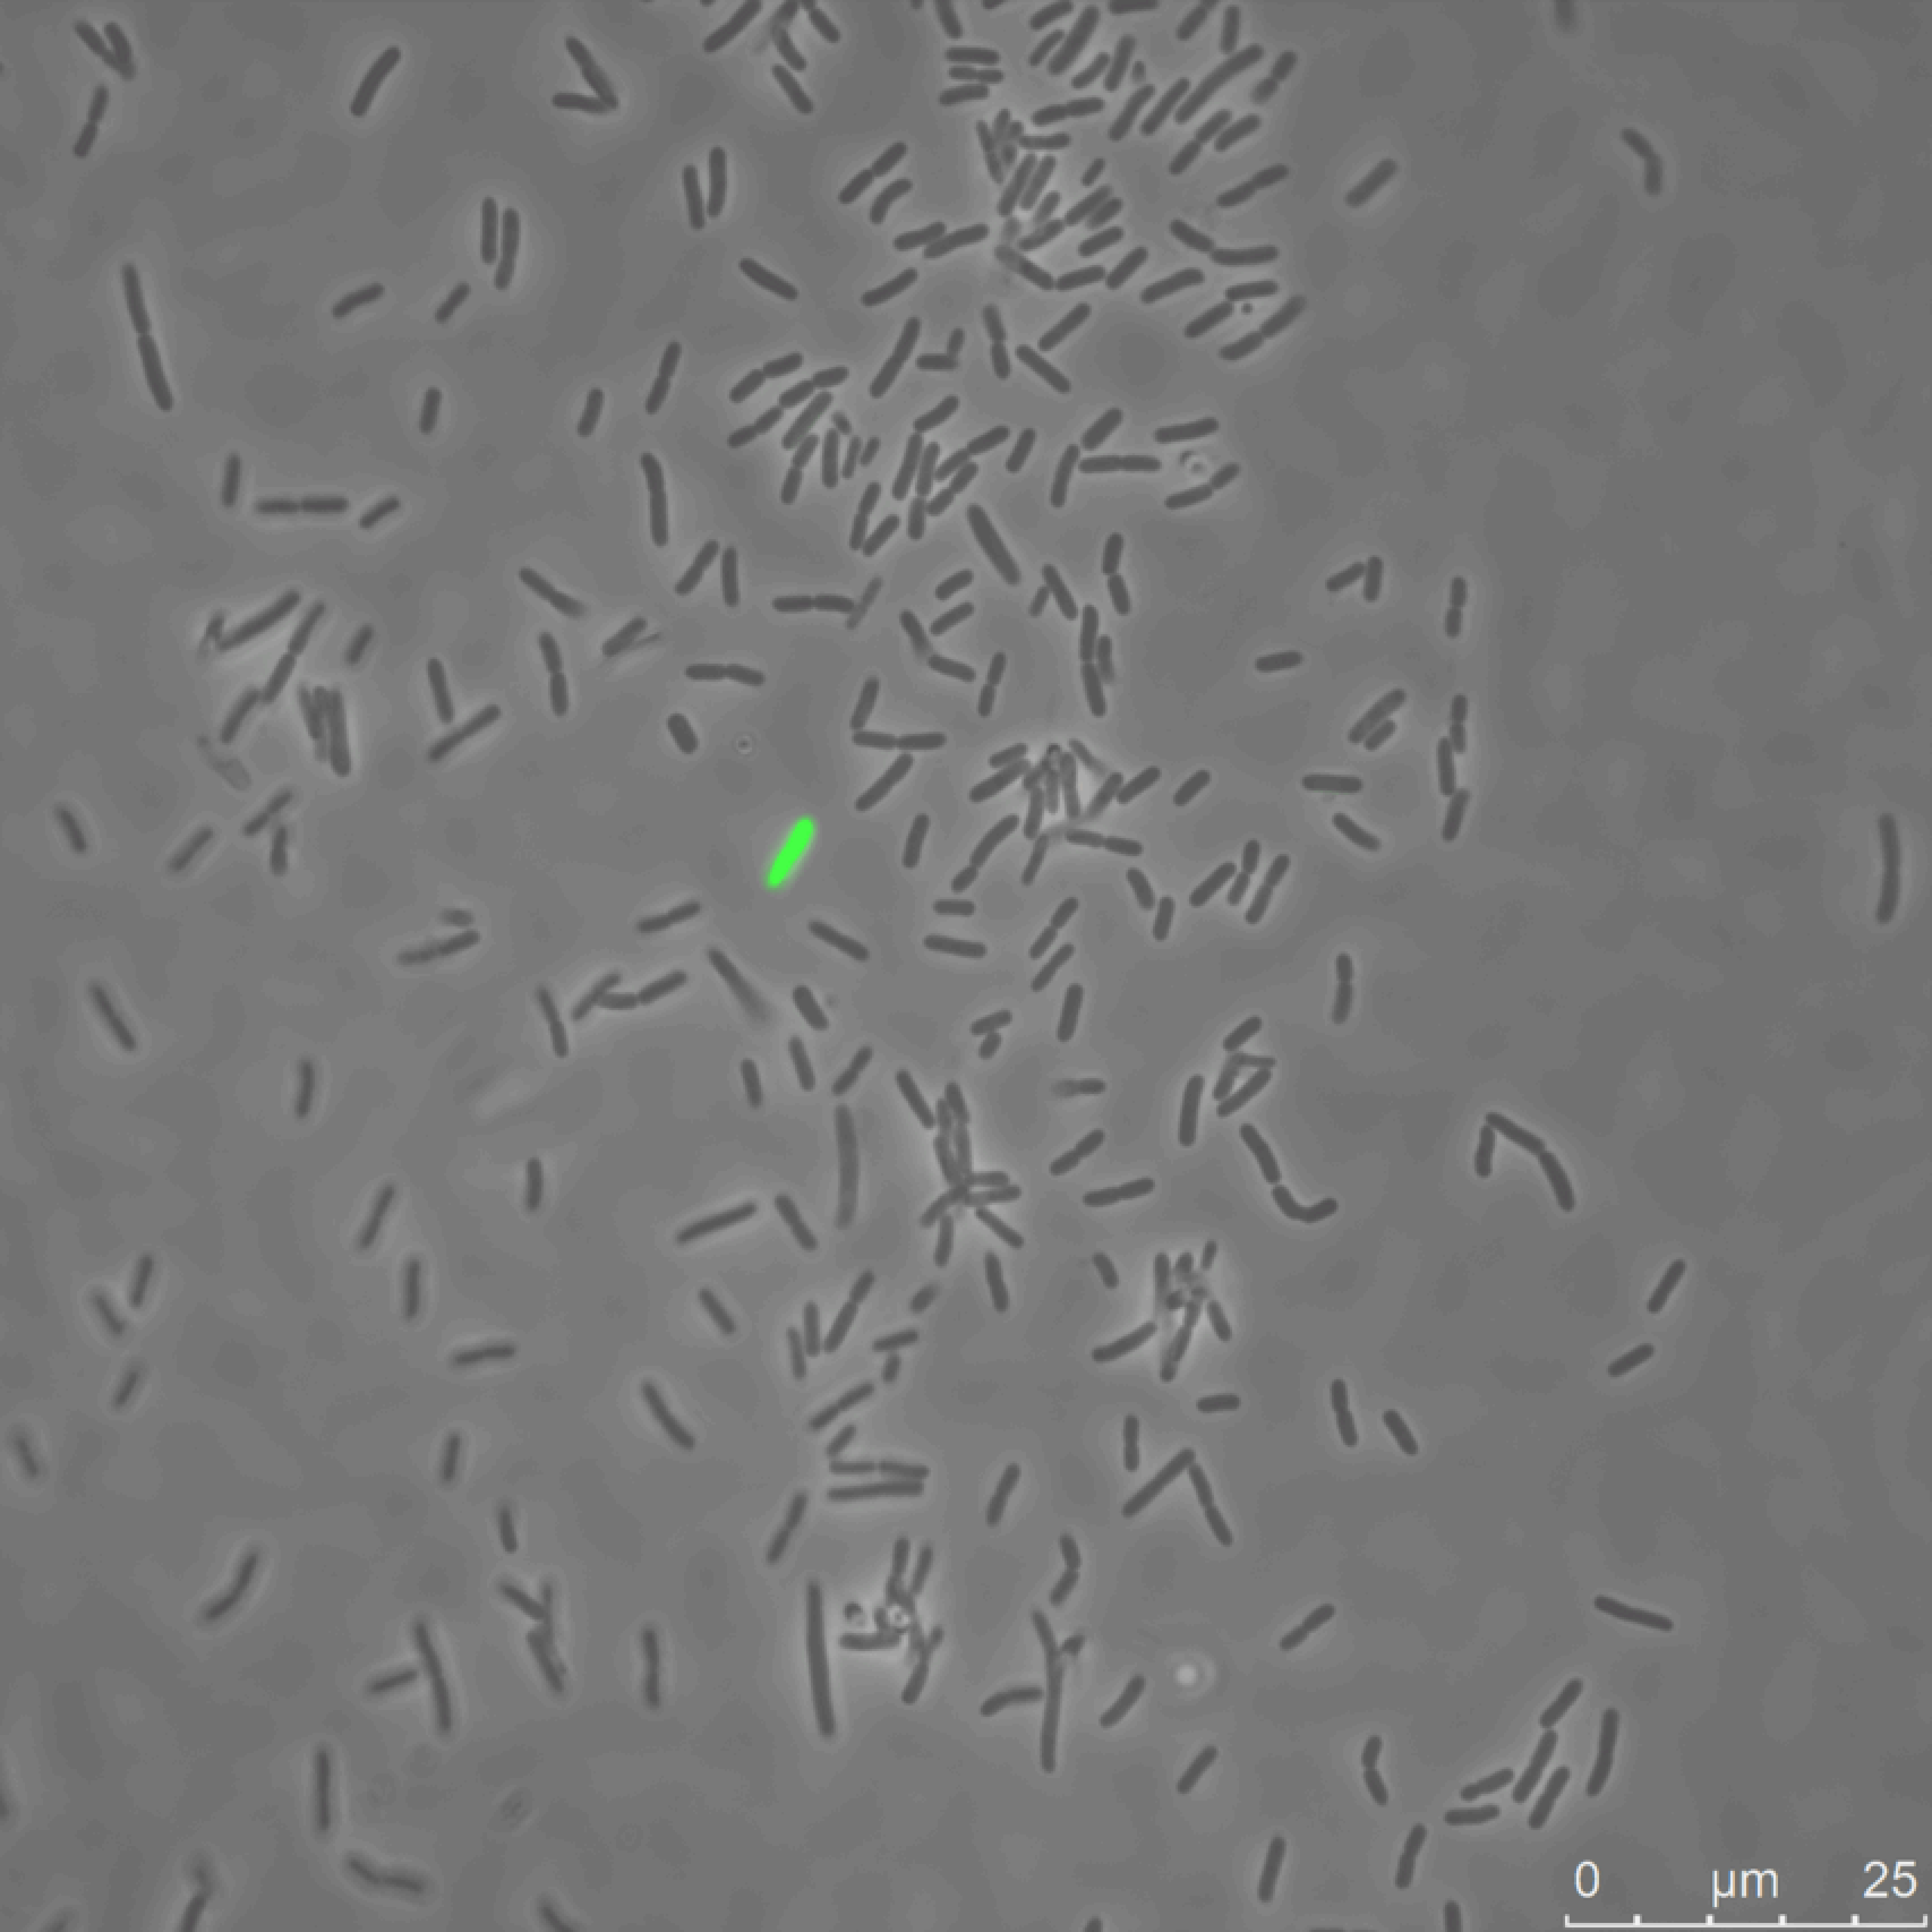
\includegraphics{TT01U4_5HR_1_GREEN-crunch-lighter-resample.pdf} &%
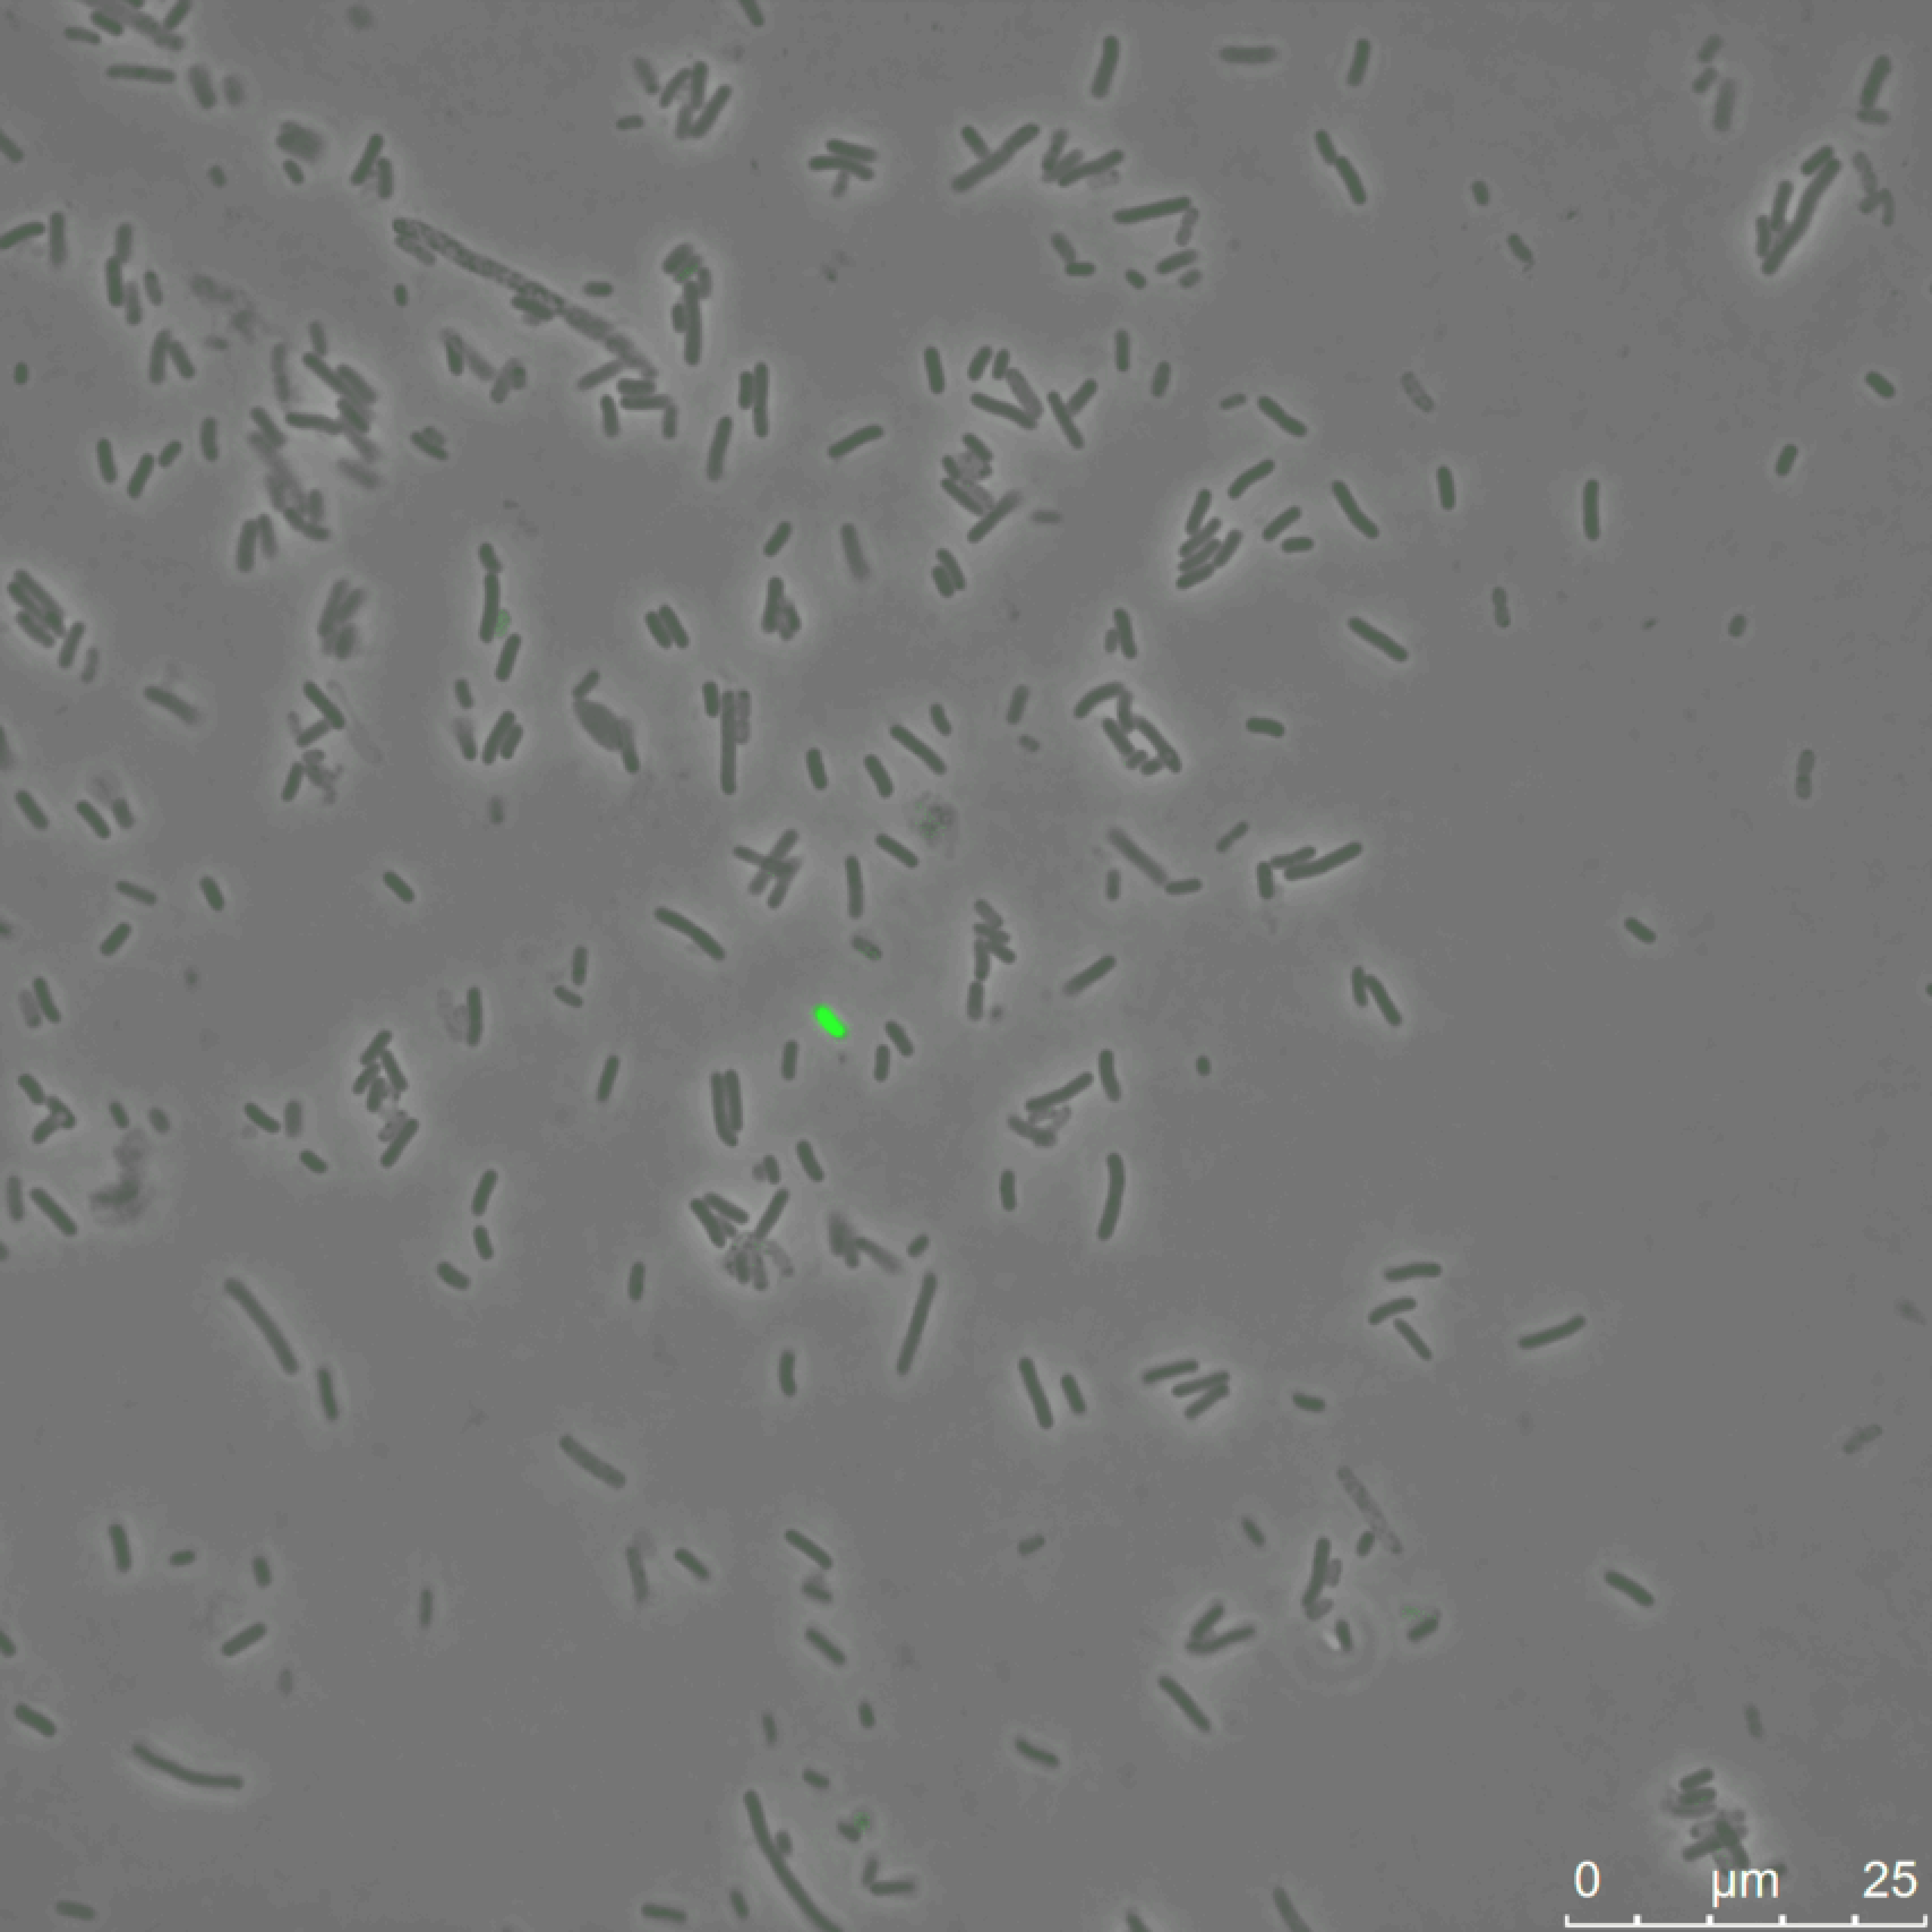
\includegraphics{TT01U4_24HR_1_GREEN-crunch-lighter-resample.pdf} &%
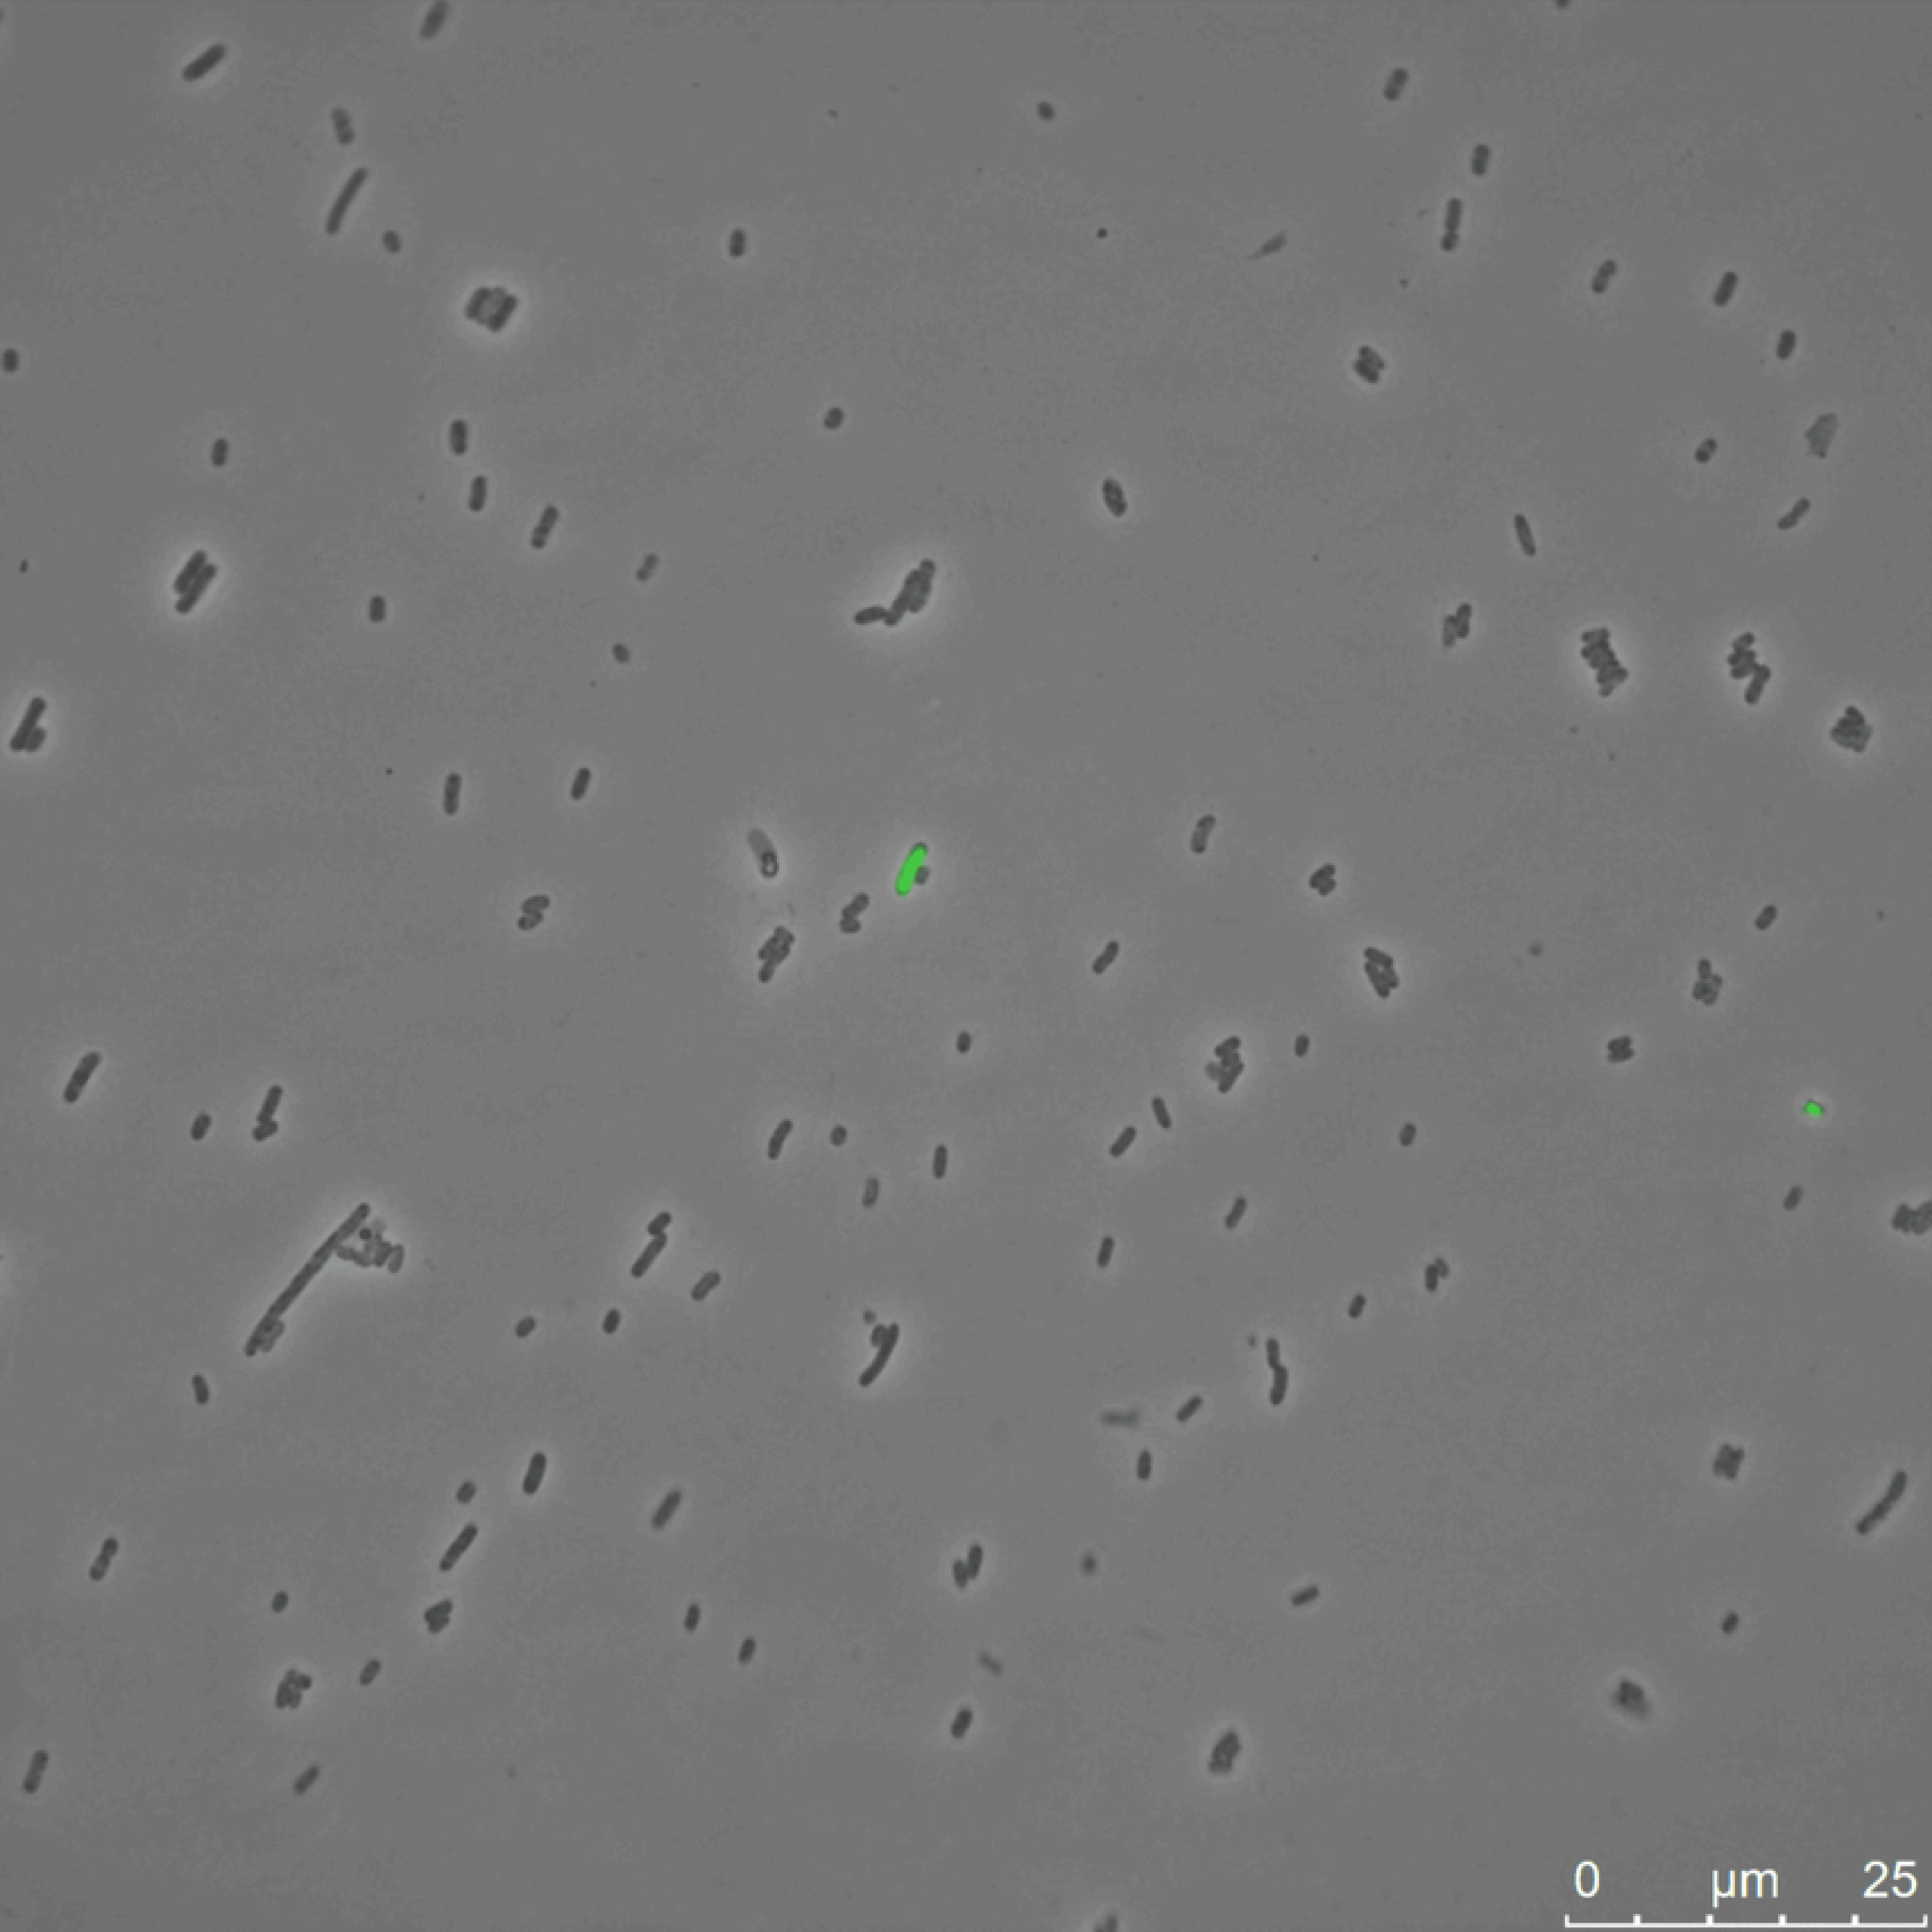
\includegraphics{TT01U4_72HR_1_GREEN-crunch-lighter-resample.pdf} \\[-0.5ex]

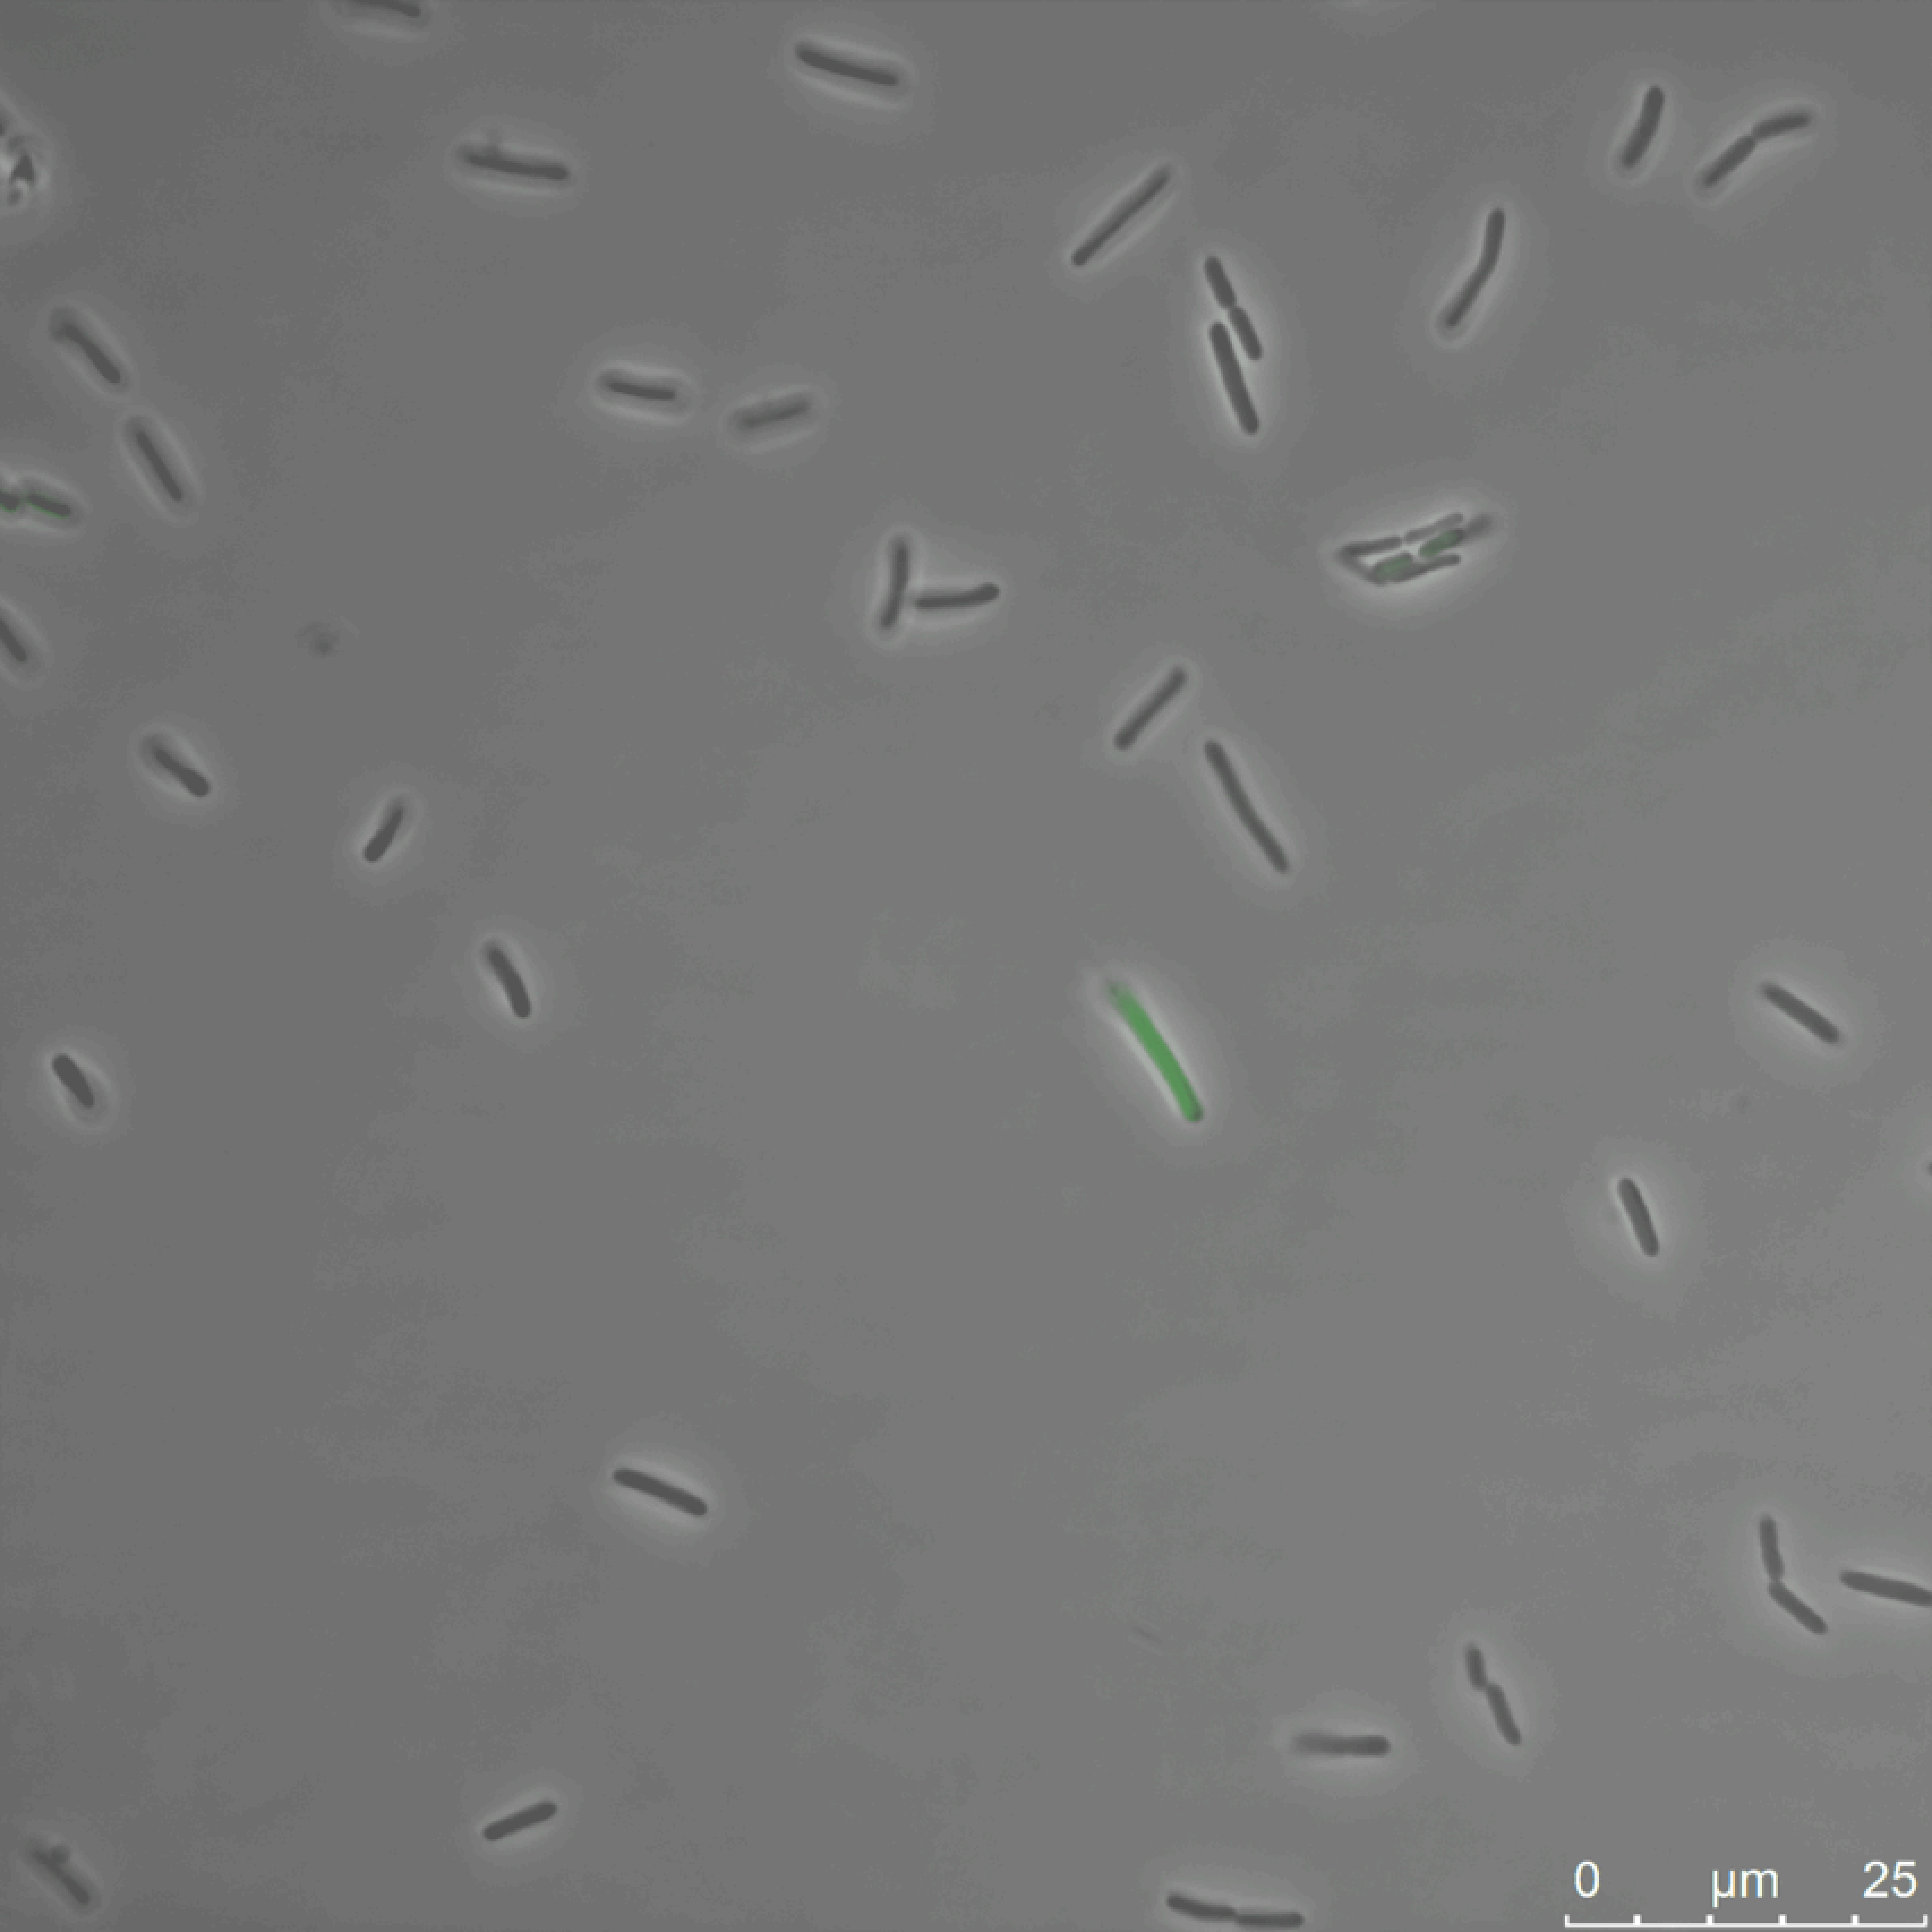
\includegraphics{TT01U4_2_GREEN-crunch-lighter-resample.pdf} &%
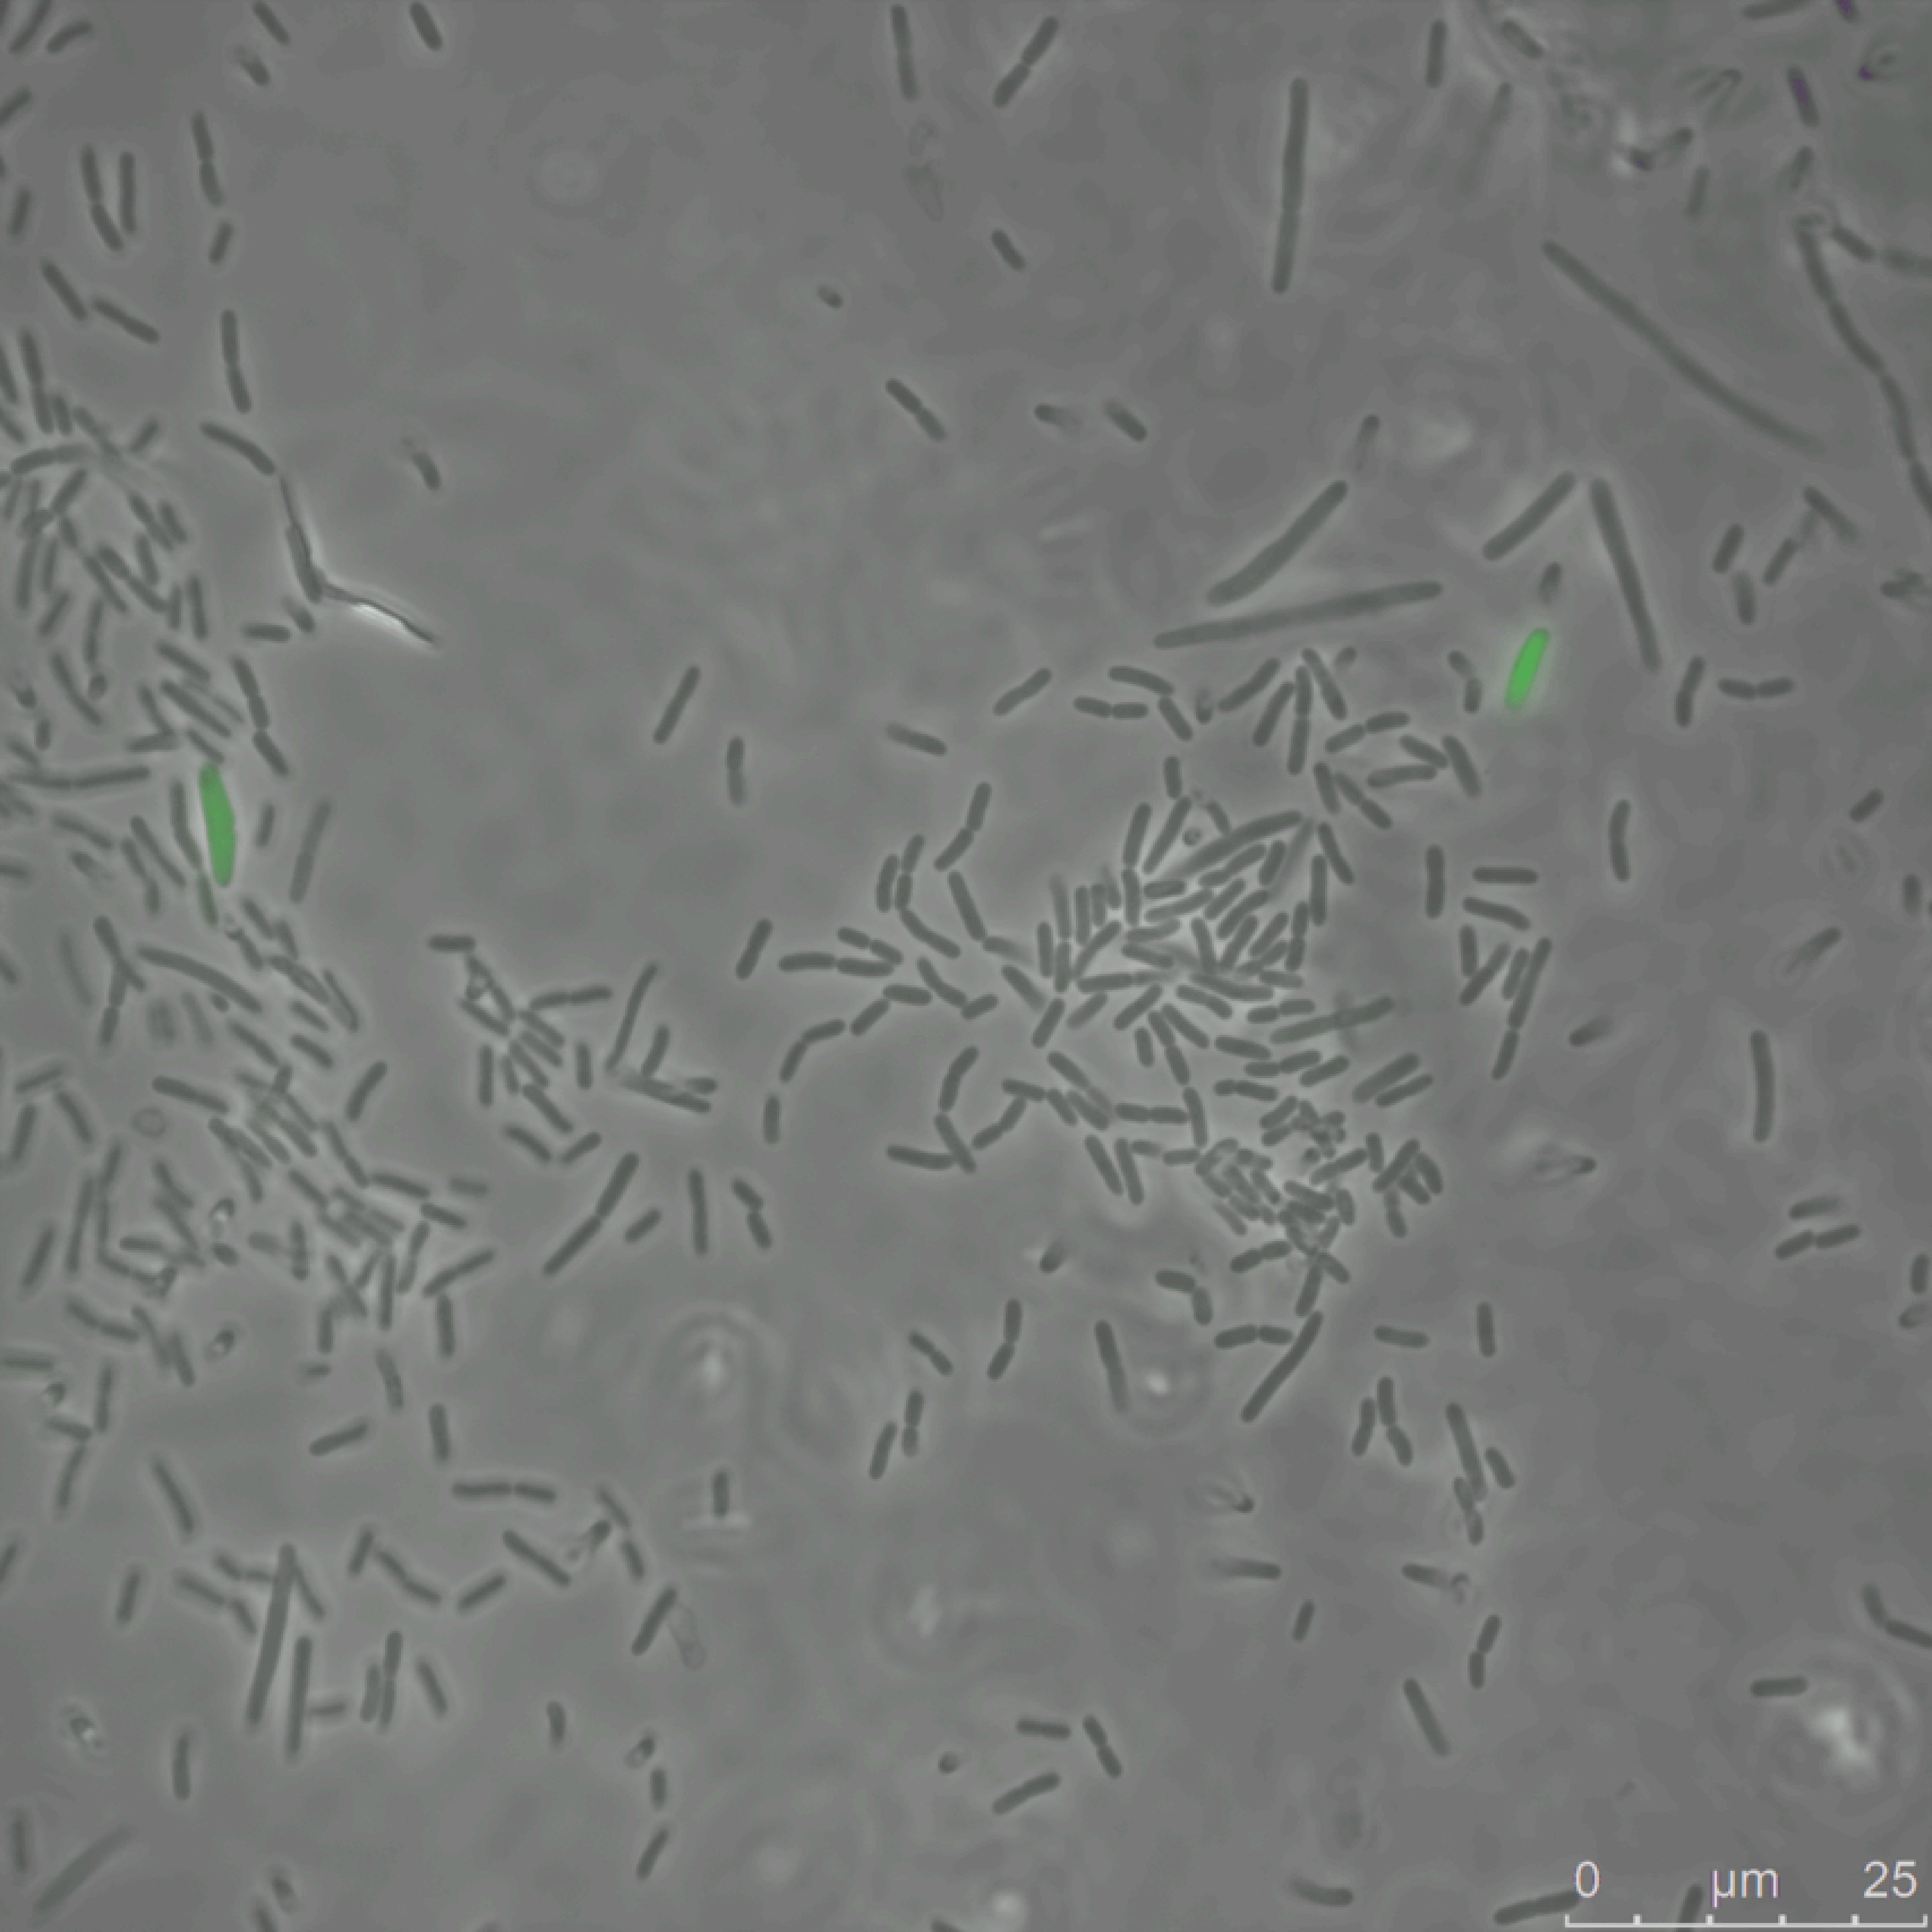
\includegraphics{TT01U4_5HR_2_GREEN-crunch-lighter-resample.pdf} &%
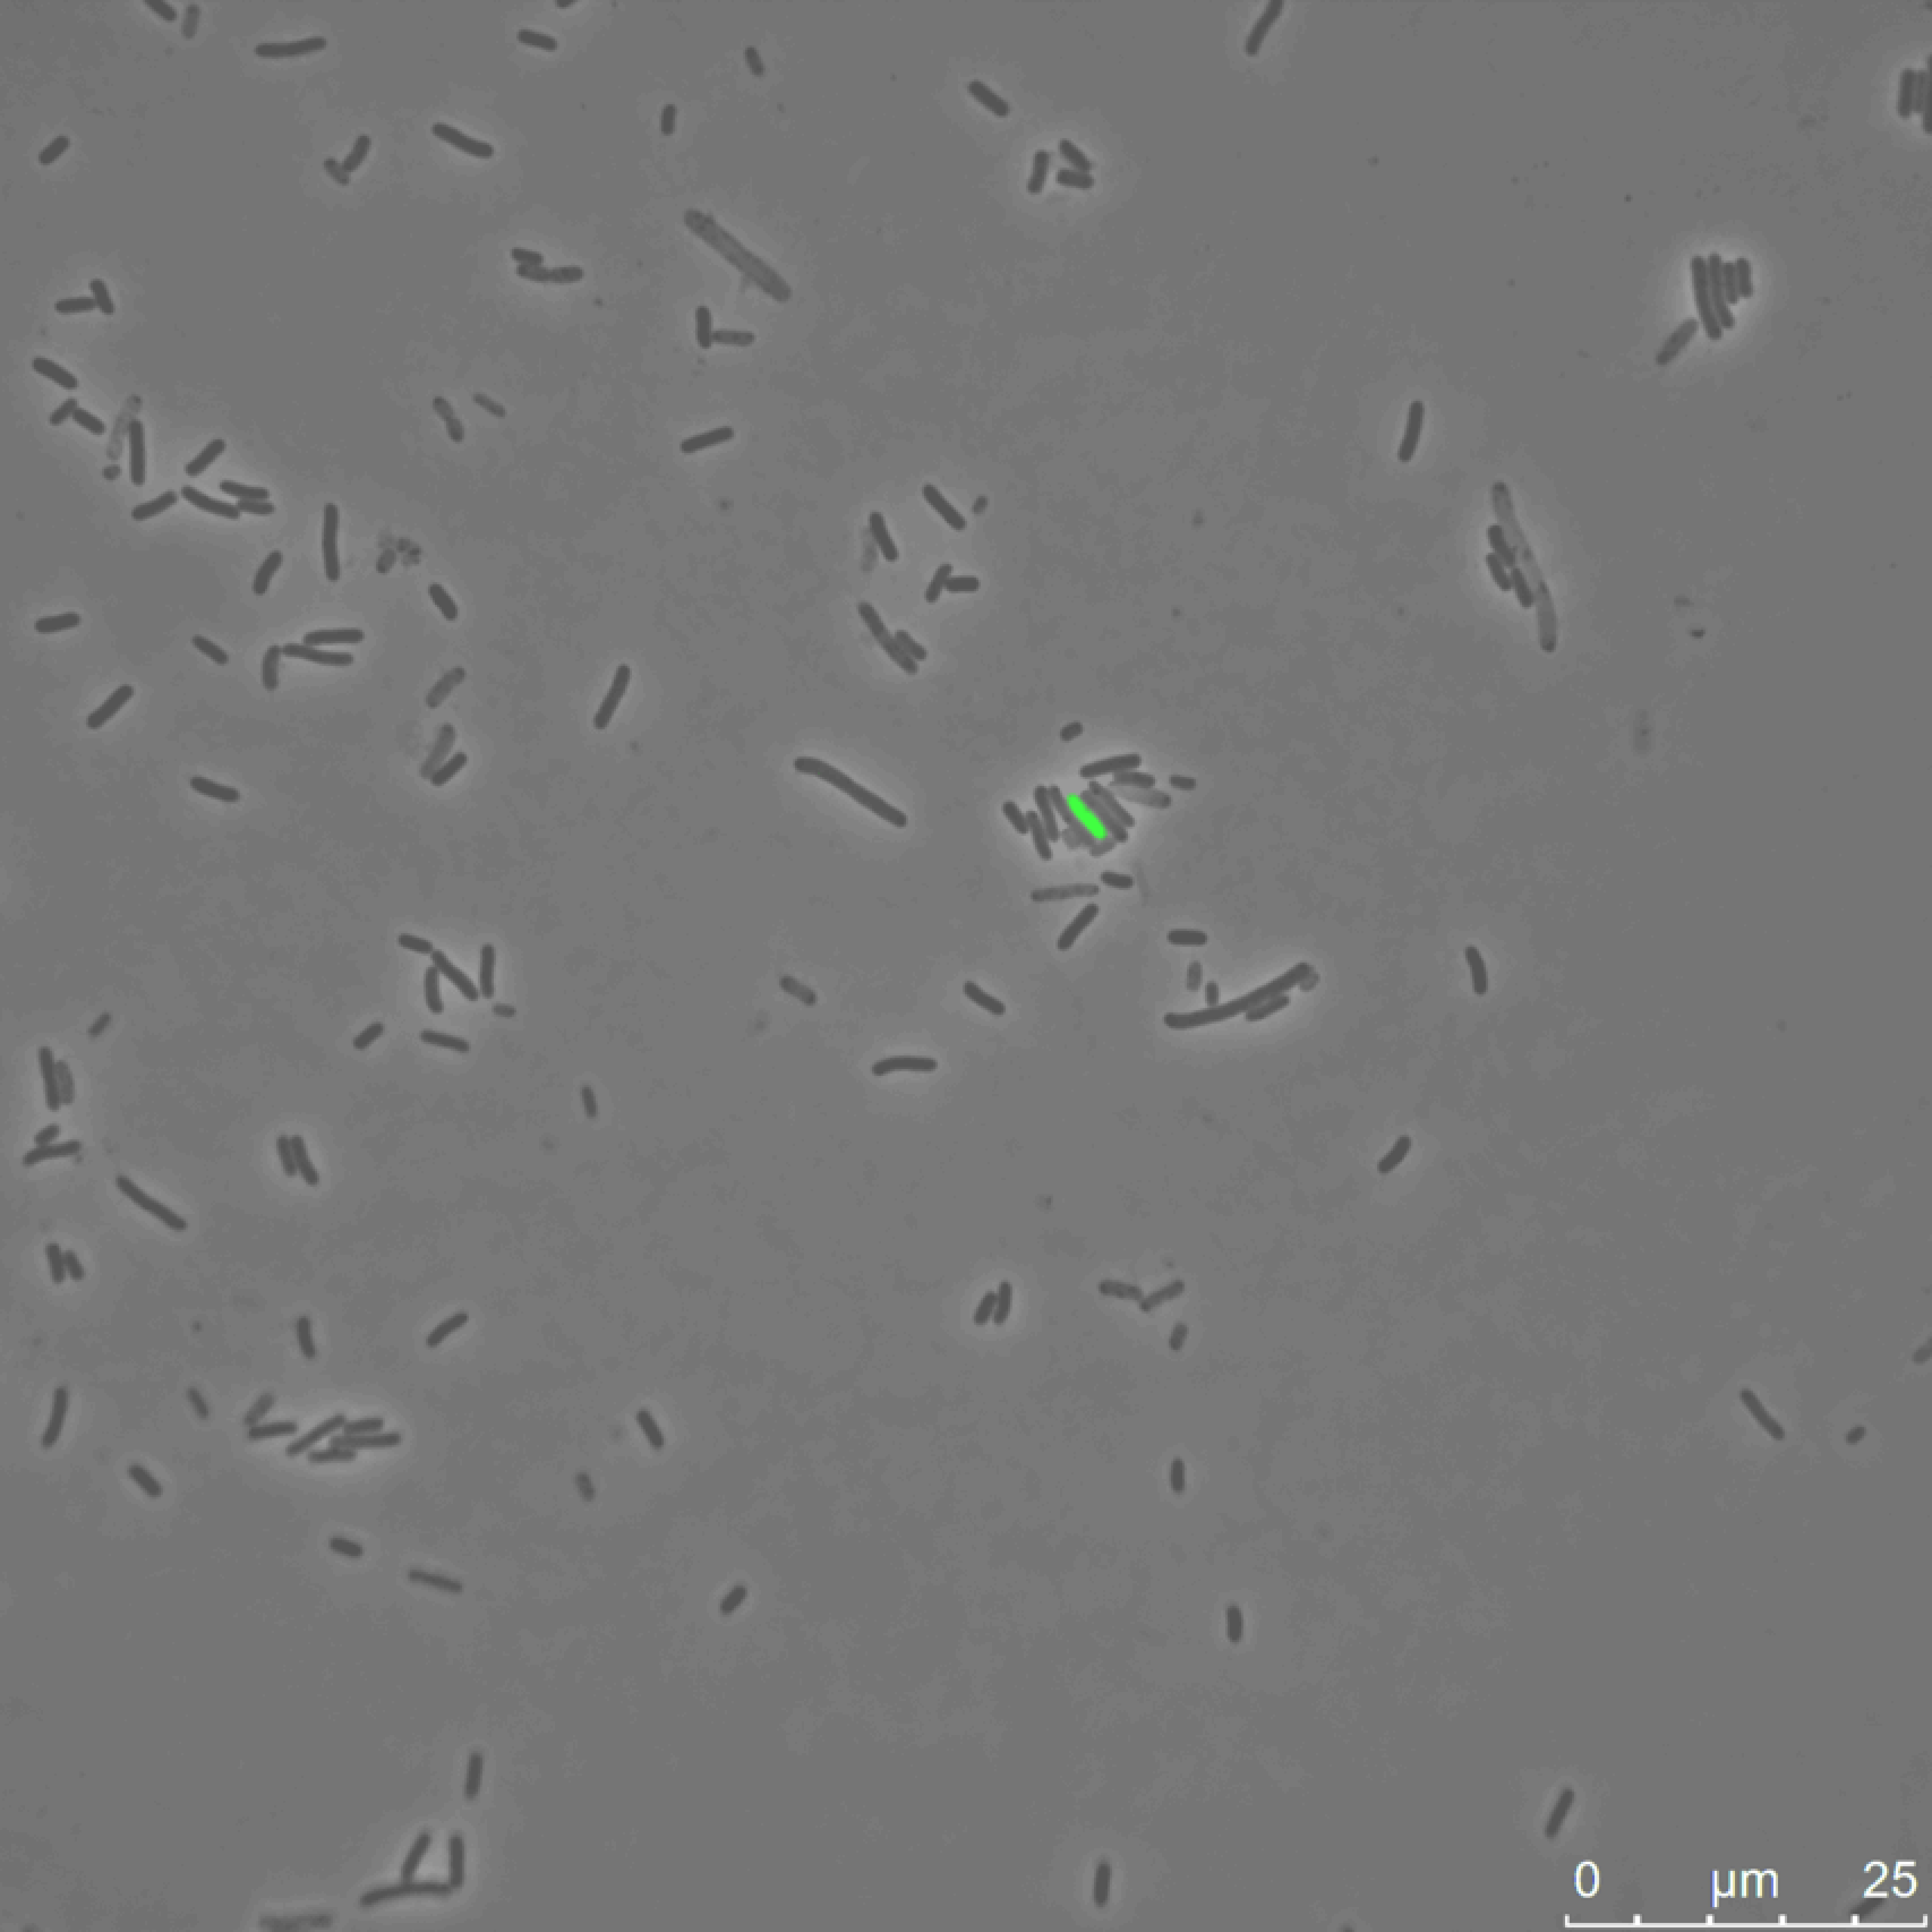
\includegraphics{TT01U4_24HR_2_GREEN-crunch-lighter-resample.pdf} &%
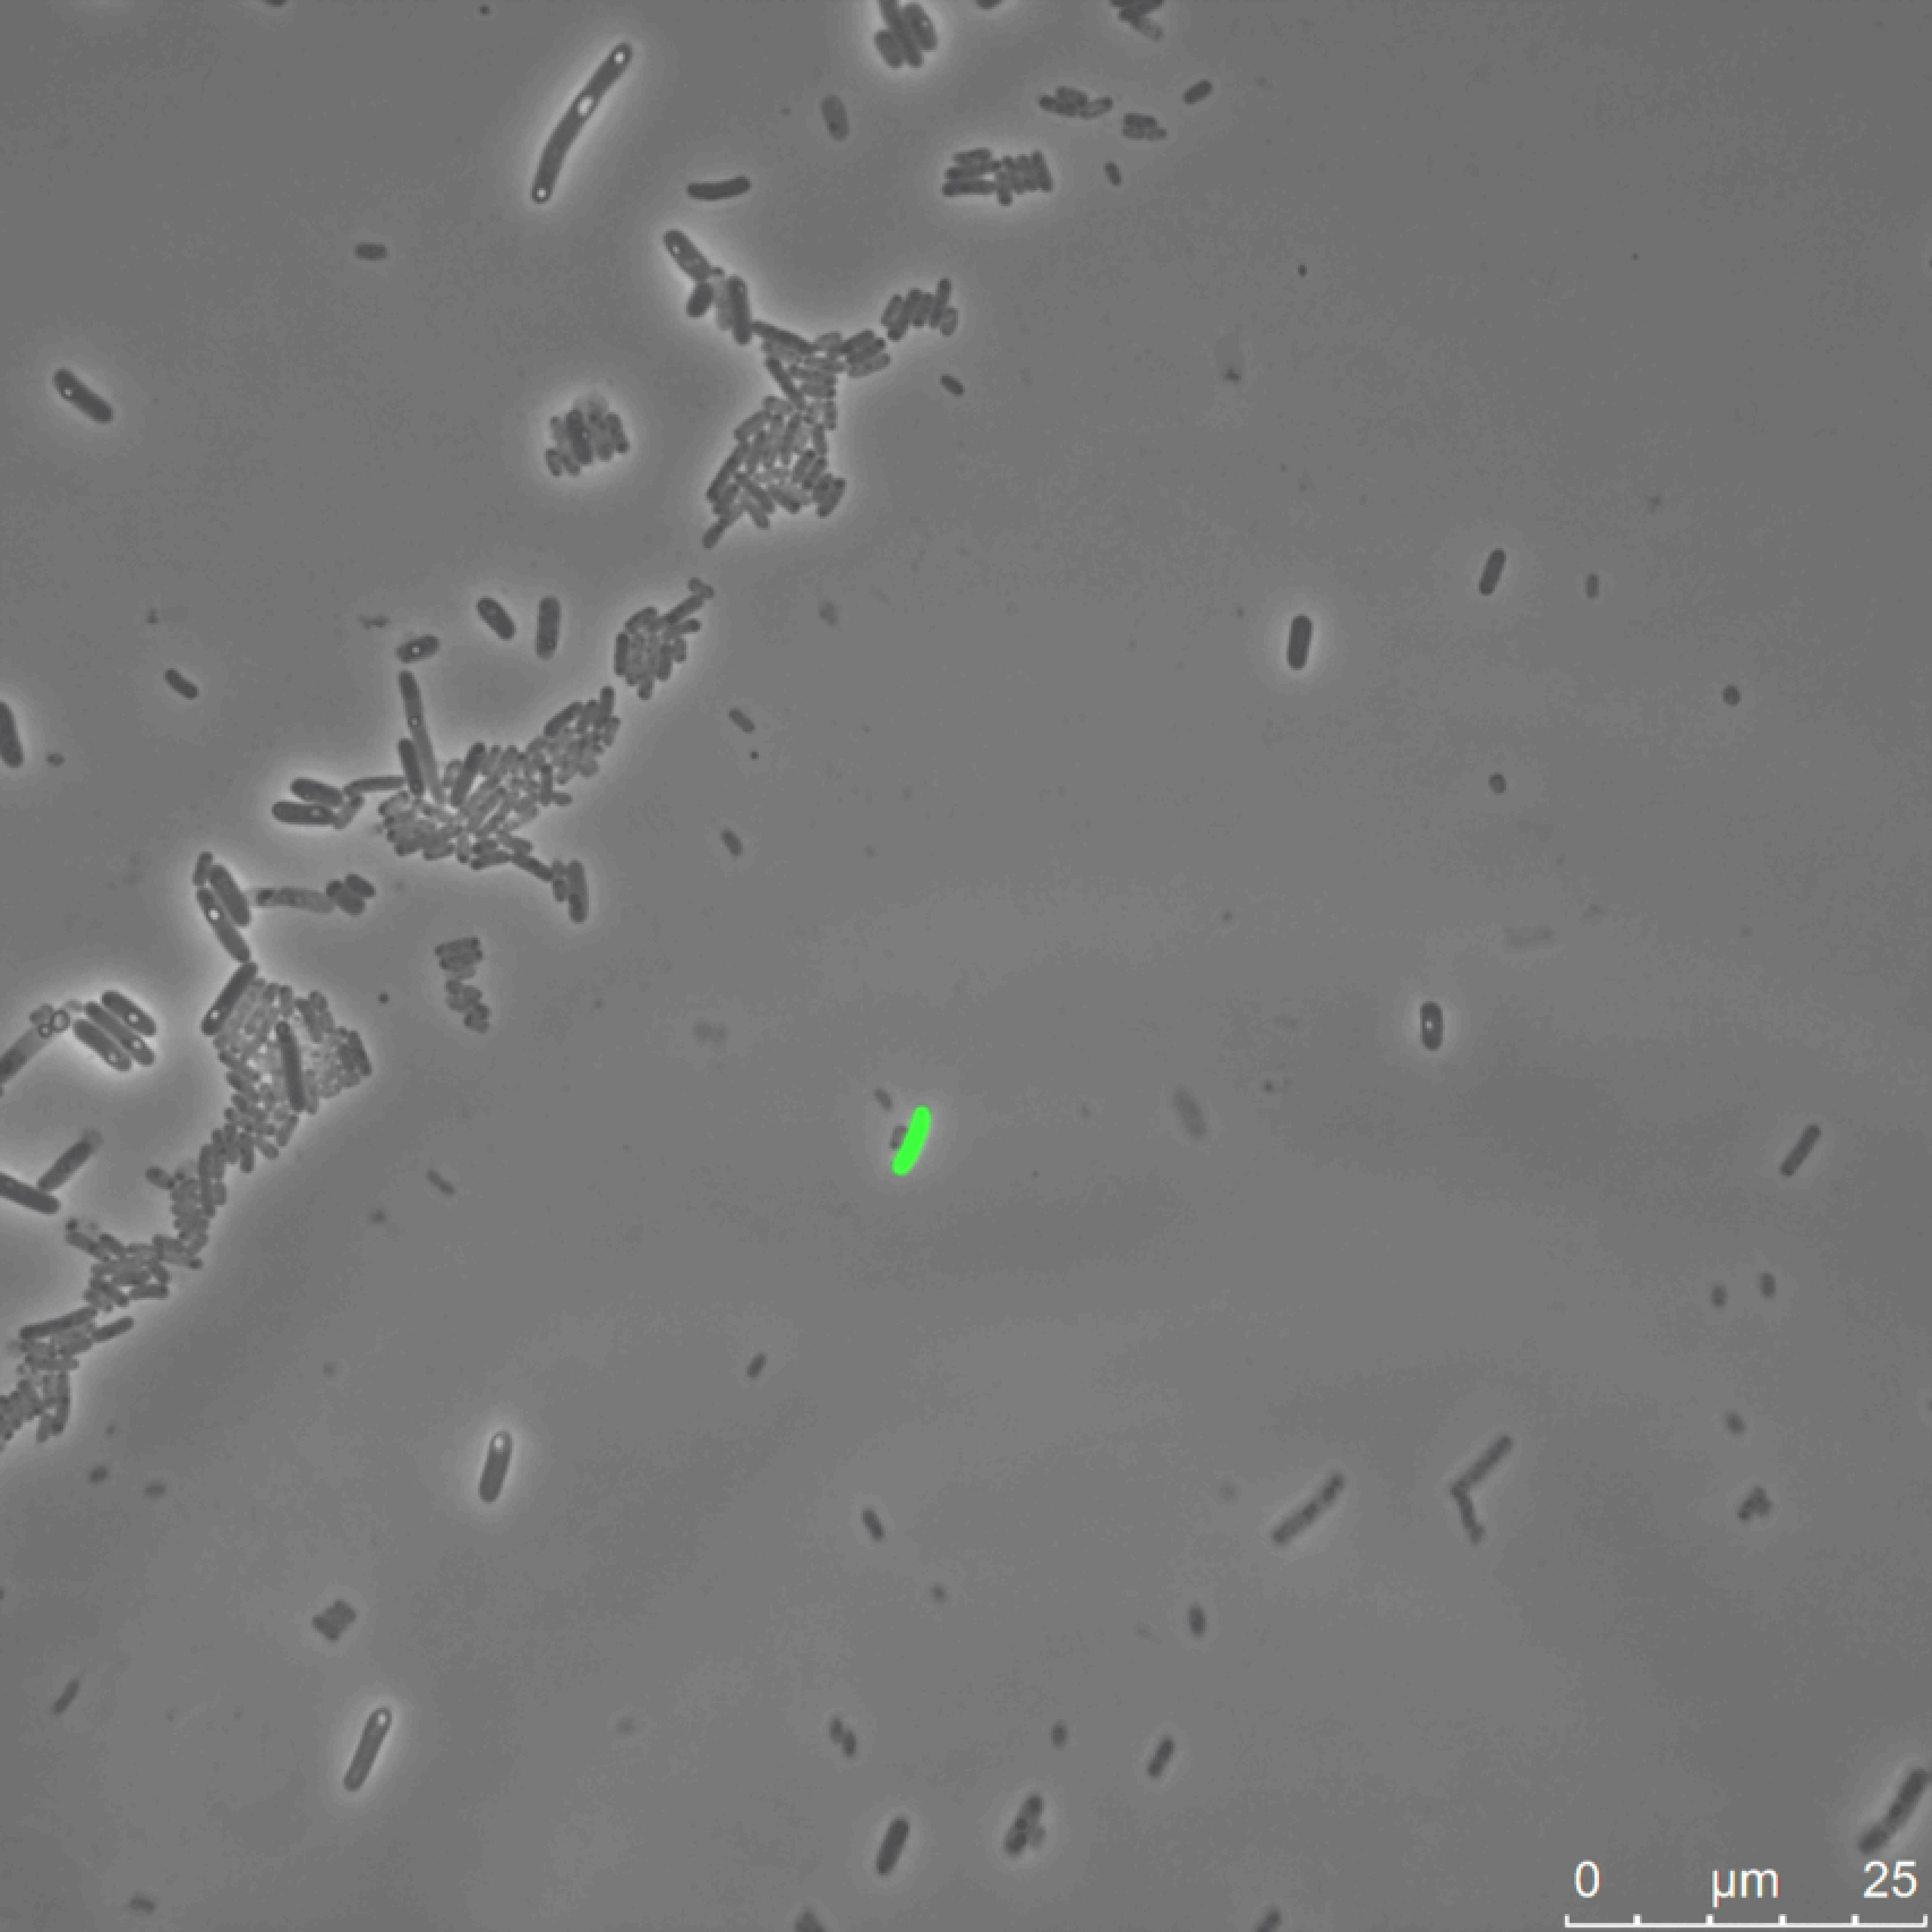
\includegraphics{TT01U4_72HR_2_GREEN-crunch-lighter-resample.pdf} \\[-0.5ex]

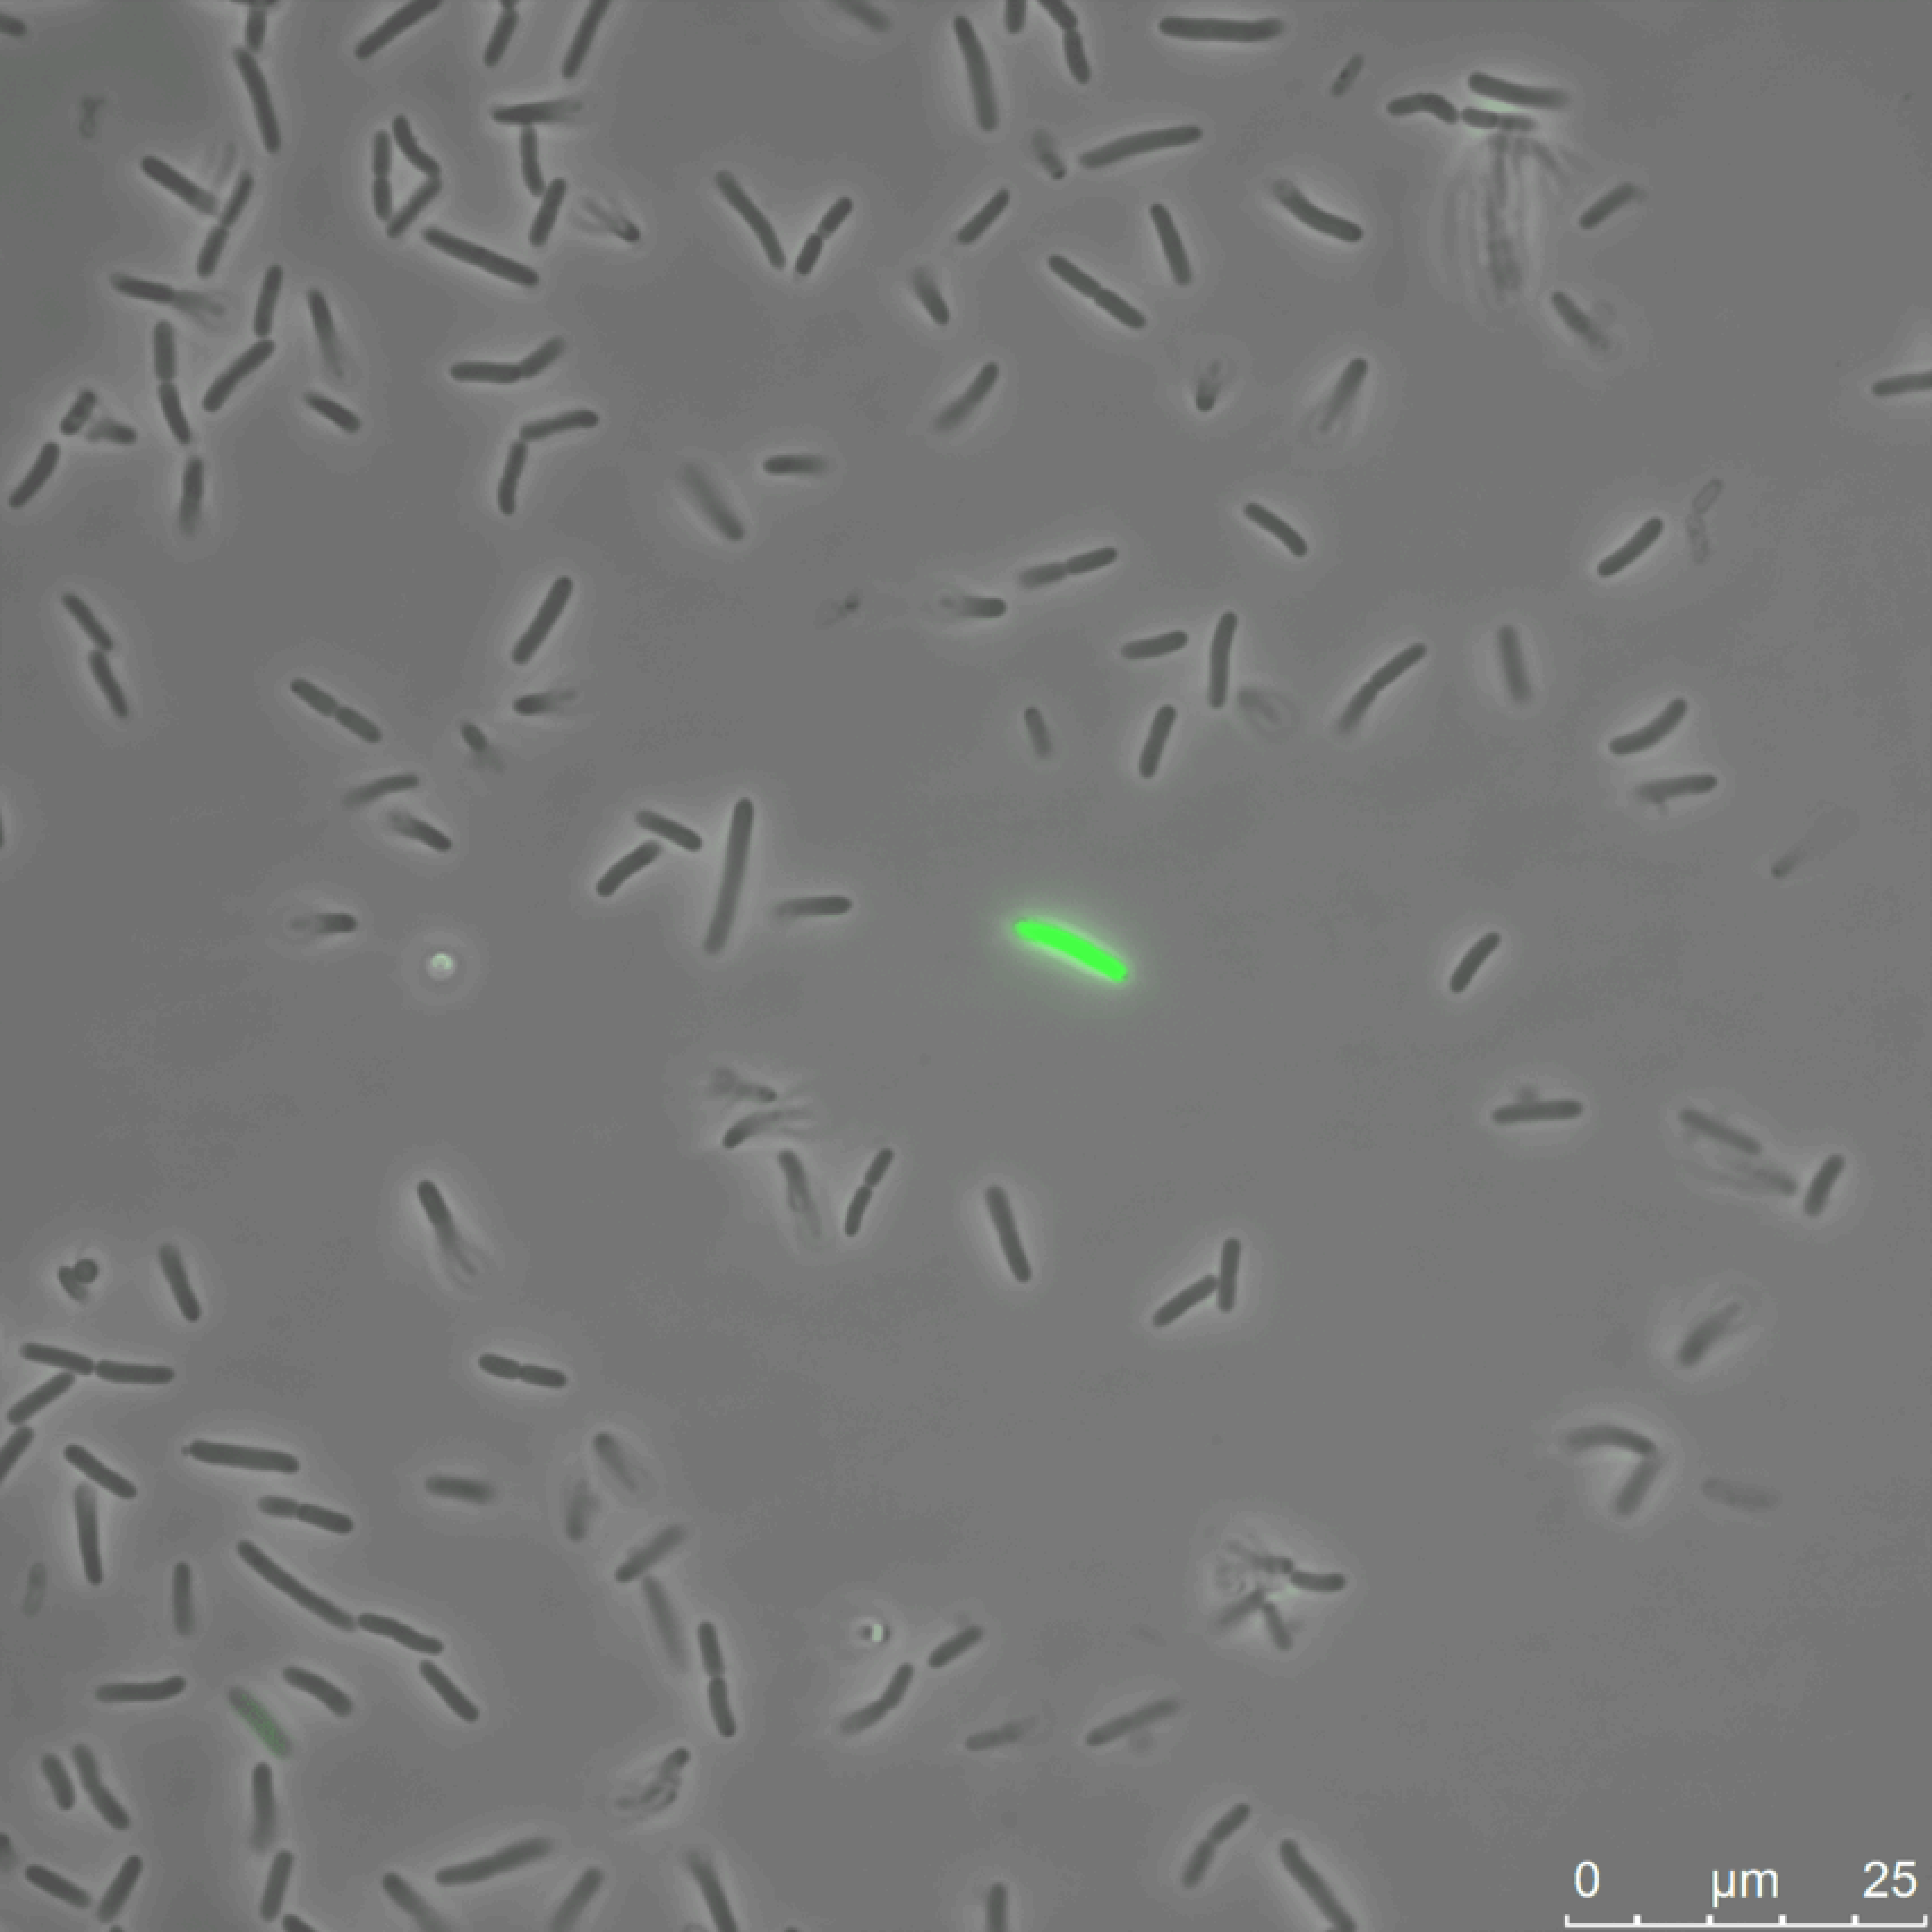
\includegraphics{TT01U4_5_GREEN-crunch-lighter-resample.pdf} &%
\includegraphics{TT01U4_5HR_3_GREEN-crunch-lighter-resample.pdf} &%
\includegraphics{TT01U4_24HR_3_GREEN-crunch-lighter-resample.pdf} &%
\includegraphics{TT01U4_72HR_3_GREEN-crunch-lighter-resample.pdf} \\[-0.5ex]

\includegraphics{TT01U4_6_GREEN-crunch-lighter-resample.pdf} &%
\includegraphics{TT01U4_5HR_4_GREEN-crunch-lighter-resample.pdf} &%
\includegraphics{TT01U4_24HR_4_GREEN-crunch-lighter-resample.pdf} &%
\includegraphics{TT01U4_72HR_4_GREEN-crunch-lighter-resample.pdf} \\
 ++ & ++ & ++ & ++ \\[1ex]

\end{tabularx}
\captionsetup{singlelinecheck=off, justification=justified, font=footnotesize, aboveskip=20pt}
\caption[Reporter microscopy - TT01 Unit 4]{\textsc{\normalsize Reporter microscopy for the \emph{P. luminescens} TT01 ``Unit 4" promoter.}\vspace{0.1cm} \newline A representative selection of images for 4 time points, for the PVC ``Unit 4" promoter fusion. Quadruplicate images are displayed vertically as representative of the whole slide sample. Key to qualitative fluorescence indication: ``-" - no fluorescence, ``+" - low level fluorescence in isolated cells. ``++" - low level fluorescence in many cells or few brighter cells, ``+++" - intermediate to high fluorescence in almost all cells, or very bright isolated cells.}
\end{figure}\label{RMTT01U4}
\endgroup

%%%%%%%%%%%%%%%%%%%%%%%%%%%%%%%%%%%%%%%%%%%%%%%%%%%%%%%%%%%%%%%%%%%%

\begingroup
\renewcommand{\arraystretch}{0.8}%
\setlength{\tabcolsep}{0.3pt}
\begin{figure}[p]
\setkeys{Gin}{width=\linewidth}
\Huge
\begin{tabularx}{\textwidth}{CCCC}
\multicolumn{4}{p{\linewidth}}{\large \centering \textbf{\emph{P. asymbiotica} PB68.1 (``THAI") PVC ``pnf"}} \\
\hiderowcolors
& & & \\[-1.5ex]
\Large 2 Hours &\Large 5 Hours &\Large 24 Hours &\Large 72 Hours \\[1ex]

\includegraphics{THAIPNF_3_GREEN-crunch-lighter-resample.pdf} &%
\includegraphics{THAIPNF_5HR_1_GREEN-crunch-lighter-resample.pdf} &%
\includegraphics{THAIPNF_24HR_2_GREEN-crunch-lighter-resample.pdf} &%
\includegraphics{THAIPNF_72HR_1_GREEN-crunch-lighter-resample.pdf} \\[-0.5ex]

\includegraphics{THAIPNF_4_GREEN-crunch-lighter-resample.pdf} &%
\includegraphics{THAIPNF_5HR_2_GREEN-crunch-lighter-resample.pdf} &%
\includegraphics{THAIPNF_24HR_4_GREEN-crunch-lighter-resample.pdf} &%
\includegraphics{THAIPNF_72HR_2_GREEN-crunch-lighter-resample.pdf} \\[-0.5ex]

\includegraphics{THAIPNF_5_GREEN-crunch-lighter-resample.pdf} &%
\includegraphics{THAIPNF_5HR_3_GREEN-crunch-lighter-resample.pdf} &%
\includegraphics{THAIPNF_24HR_5_GREEN-crunch-lighter-resample.pdf} &%
\includegraphics{THAIPNF_72HR_3_GREEN-crunch-lighter-resample.pdf} \\[-0.5ex]

\includegraphics{THAIPNF_6_GREEN-crunch-lighter-resample.pdf} &%
\includegraphics{THAIPNF_5HR_4_GREEN-crunch-lighter-resample.pdf} &%
\includegraphics{THAIPNF_24HR_7_GREEN-crunch-lighter-resample.pdf} &%
\includegraphics{THAIPNF_72HR_4_GREEN-crunch-lighter-resample.pdf} \\
 ++ & ++ & +++ & +++ \\[1ex]

\end{tabularx}

\captionsetup{singlelinecheck=off, justification=justified, font=footnotesize, aboveskip=20pt}
\caption[Reporter microscopy - PB68.1 pnf]{\textsc{\normalsize Reporter microscopy for the \emph{P. asymbiotica} PB68.1 ``pnf" promoter.}\vspace{0.1cm} \newline A representative selection of images for 4 time points, for the PVC ``pnf" promoter fusion. Quadruplicate images are displayed vertically as representative of the whole slide sample. Key to qualitative fluorescence indication: ``-" - no fluorescence, ``+" - low level fluorescence in isolated cells. ``++" - low level fluorescence in many cells or few brighter cells, ``+++" - intermediate to high fluorescence in almost all cells, or very bright isolated cells.}
\end{figure}\label{RMTHAIPNF}
\endgroup

%%%%%%%%%%%%%%%%%%%%%%%%%%%%%%%%%%%%%%%%%%%%%%%%%%%%%%%%%%%%%%%%%%%%

\begingroup
\renewcommand{\arraystretch}{0.8}%
\setlength{\tabcolsep}{0.3pt}
\begin{figure}[p]
\setkeys{Gin}{width=\linewidth}
\Huge
\begin{tabularx}{\textwidth}{CCCC}
\multicolumn{4}{p{\linewidth}}{\large \centering \textbf{\emph{P. luminescens} TT01 PVC ``LopT"}} \\
\hiderowcolors
& & & \\[-1.5ex]
\Large 2 Hours &\Large 5 Hours &\Large 24 Hours &\Large 72 Hours \\[1ex]

\includegraphics{TT01LOPT_1_LOWGREEN-crunch-lighter-resample.pdf} &%
\includegraphics{TT01LOPT_5HR_1_LOWGREEN-crunch-lighter-resample.pdf} &%
\includegraphics{TT01LOPT_24HR_1_GREEN-crunch-lighter-resample.pdf} &%
\includegraphics{TT01LOPT_72HR_1_GREEN-crunch-lighter-resample.pdf} \\[-0.5ex]

\includegraphics{TT01LOPT_2_NOGREEN-crunch-lighter-resample.pdf} &%
\includegraphics{TT01LOPT_5HR_2_LOWGREEN-crunch-lighter-resample.pdf} &%
\includegraphics{TT01LOPT_24HR_2_GREEN-crunch-lighter-resample.pdf} &%
\includegraphics{TT01LOPT_72HR_2_GREEN-crunch-lighter-resample.pdf} \\[-0.5ex]

\includegraphics{TT01LOPT_3_LOWGREEN-crunch-lighter-resample.pdf} &%
\includegraphics{TT01LOPT_5HR_3_LOWGREEN-crunch-lighter-resample.pdf} &%
\includegraphics{TT01LOPT_24HR_3_GREEN-crunch-lighter-resample.pdf} &%
\includegraphics{TT01LOPT_72HR_3_GREEN-crunch-lighter-resample.pdf} \\[-0.5ex]

\includegraphics{TT01LOPT_4_LOWGREEN-crunch-lighter-resample.pdf} &%
\includegraphics{TT01LOPT_5HR_4_LOWGREEN-crunch-lighter-resample.pdf} &%
\includegraphics{TT01LOPT_24HR_7_GREEN-crunch-lighter-resample.pdf} &%
\includegraphics{TT01LOPT_72HR_6_GREEN-crunch-lighter-resample.pdf} \\
 + & + & ++ & ++ \\[1ex]

\end{tabularx}

\captionsetup{singlelinecheck=off, justification=justified, font=footnotesize, aboveskip=20pt}
\caption[Reporter microscopy - TT01 LopT]{\textsc{\normalsize Reporter microscopy for the \emph{P. luminescens} TT01 ``LopT" promoter.}\vspace{0.1cm} \newline A representative selection of images for 4 time points, for the PVC ``LopT" promoter fusion. Quadruplicate images are displayed vertically as representative of the whole slide sample. Key to qualitative fluorescence indication: ``-" - no fluorescence, ``+" - low level fluorescence in isolated cells. ``++" - low level fluorescence in many cells or few brighter cells, ``+++" - intermediate to high fluorescence in almost all cells, or very bright isolated cells.}
\end{figure}\label{RMTT01LOPT}
\endgroup

%%%%%%%%%%%%%%%%%%%%%%%%%%%%%%%%%%%%%%%%%%%%%%%%%%%%%%%%%%%%%%%%%%%%


\begingroup
\renewcommand{\arraystretch}{0.8}%
\setlength{\tabcolsep}{0.3pt}
\begin{figure}[p]
\setkeys{Gin}{width=\linewidth}
\Huge
\begin{tabularx}{\textwidth}{CCCC}
\multicolumn{4}{p{\linewidth}}{\large \centering \textbf{\emph{P. asymbiotica} PB68.1 (``THAI") PVC ``LopT"}} \\
\hiderowcolors
& & & \\[-1.5ex]
\Large 2 Hours &\Large 5 Hours &\Large 24 Hours &\Large 72 Hours \\[1ex]

\includegraphics{THAILOPT_1_NOGREEN-crunch-lighter-resample.pdf} &%
\includegraphics{THAILOPT_5HR_1_NOGREEN-crunch-lighter-resample.pdf} &%
\includegraphics{THAILOPT_24HR_1_NOGREEN-crunch-lighter-resample.pdf} &%
\includegraphics{THAILOPT_72HR_1_NOGREEN-crunch-lighter-resample.pdf} \\[-0.5ex]

\includegraphics{THAILOPT_2_NOGREEN-crunch-lighter-resample.pdf} &%
\includegraphics{THAILOPT_5HR_2_NOGREEN-crunch-lighter-resample.pdf} &%
\includegraphics{THAILOPT_24HR_2_NOGREEN-crunch-lighter-resample.pdf} &%
\includegraphics{THAILOPT_72HR_2_NOGREEN-crunch-lighter-resample.pdf} \\[-0.5ex]

\includegraphics{THAILOPT_3_NOGREEN-crunch-lighter-resample.pdf} &%
\includegraphics{THAILOPT_5HR_3_NOGREEN-crunch-lighter-resample.pdf} &%
\includegraphics{THAILOPT_24HR_3_NOGREEN-crunch-lighter-resample.pdf} &%
\includegraphics{THAILOPT_72HR_3_NOGREEN-crunch-lighter-resample.pdf} \\[-0.5ex]

\includegraphics{THAILOPT_4_NOGREEN-crunch-lighter-resample.pdf} &%
\includegraphics{THAILOPT_5HR_4_NOGREEN-crunch-lighter-resample.pdf} &%
\includegraphics{THAILOPT_24HR_4_NOGREEN-crunch-lighter-resample.pdf} &%
\includegraphics{THAILOPT_72HR_4_NOGREEN-crunch-lighter-resample.pdf} \\
 - & - & - & - \\[1ex]

\end{tabularx}
\captionsetup{singlelinecheck=off, justification=justified, font=footnotesize, aboveskip=20pt}
\caption[Reporter microscopy - PB68.1 LopT]{\textsc{\normalsize Reporter microscopy for the \emph{P. asymbiotica} PB68.1 ``LopT" promoter.}\vspace{0.1cm} \newline A representative selection of images for 4 time points, for the PVC ``LopT" promoter fusion. Quadruplicate images are displayed vertically as representative of the whole slide sample. Key to qualitative fluorescence indication: ``-" - no fluorescence, ``+" - low level fluorescence in isolated cells. ``++" - low level fluorescence in many cells or few brighter cells, ``+++" - intermediate to high fluorescence in almost all cells, or very bright isolated cells.}
\end{figure}\label{RMTHAILOPT}
\endgroup

%%%%%%%%%%%%%%%%%%%%%%%%%%%%%%%%%%%%%%%%%%%%%%%%%%%%%%%%%%%%%%%%%%%%


\begingroup
\renewcommand{\arraystretch}{0.8}%
\setlength{\tabcolsep}{0.3pt}
\begin{figure}[p]
\setkeys{Gin}{width=\linewidth}
\Huge
\begin{tabularx}{\textwidth}{CCCC}
\multicolumn{4}{p{\linewidth}}{\large \centering \textbf{\emph{P. luminescens} TT01 PVC ``Cif"}} \\
\hiderowcolors
& & & \\[-1.5ex]
\Large 2 Hours &\Large 5 Hours &\Large 24 Hours &\Large 72 Hours \\[1ex]

\includegraphics{TT01CIF_1_NOGREEN-crunch-lighter-resample.pdf} &%
\includegraphics{TT01CIF_5HR_1_LOWGREEN-crunch-lighter-resample.pdf} &%
\includegraphics{TT01CIF_24HR_6_GREEN-crunch-lighter-resample.pdf} &%
\includegraphics{TT01CIF_72HR_5_GREEN-crunch-lighter-resample.pdf} \\[-0.5ex]

\includegraphics{TT01CIF_2_NOGREEN-crunch-lighter-resample.pdf} &%
\includegraphics{TT01CIF_5HR_2_LOWGREEN-crunch-lighter-resample.pdf} &%
\includegraphics{TT01CIF_24HR_2_GREEN-crunch-lighter-resample.pdf} &%
\includegraphics{TT01CIF_72HR_7_GREEN-crunch-lighter-resample.pdf} \\[-0.5ex]

\includegraphics{TT01CIF_3_NOGREEN-crunch-lighter-resample.pdf} &%
\includegraphics{TT01CIF_5HR_3_LOWGREEN-crunch-lighter-resample.pdf} &%
\includegraphics{TT01CIF_24HR_3_GREEN-crunch-lighter-resample.pdf} &%
\includegraphics{TT01CIF_72HR_3_GREEN-crunch-lighter-resample.pdf} \\[-0.5ex]

\includegraphics{TT01CIF_4_LOWGREEN-crunch-lighter-resample.pdf} &%
\includegraphics{TT01CIF_5HR_5_LOWGREEN-crunch-lighter-resample.pdf} &%
\includegraphics{TT01CIF_24HR_4_GREEN-crunch-lighter-resample.pdf} &%
\includegraphics{TT01CIF_72HR_6_GREEN-crunch-lighter-resample.pdf} \\
 - & + & ++ & ++ \\[1ex]

\end{tabularx}
\captionsetup{singlelinecheck=off, justification=justified, font=footnotesize, aboveskip=20pt}
\caption[Reporter microscopy - TT01 Cif]{\textsc{\normalsize Reporter microscopy for the \emph{P. luminescens} TT01 ``Cif" promoter.}\vspace{0.1cm} \newline A representative selection of images for 4 time points, for the PVC ``Cif" promoter fusion. Quadruplicate images are displayed vertically as representative of the whole slide sample. Key to qualitative fluorescence indication: ``-" - no fluorescence, ``+" - low level fluorescence in isolated cells. ``++" - low level fluorescence in many cells or few brighter cells, ``+++" - intermediate to high fluorescence in almost all cells, or very bright isolated cells.}
\end{figure}\label{RMTT01CIF}
\endgroup

%%%%%%%%%%%%%%%%%%%%%%%%%%%%%%%%%%%%%%%%%%%%%%%%%%%%%%%%%%%%%%%%%%%%


\begingroup
\renewcommand{\arraystretch}{0.8}%
\setlength{\tabcolsep}{0.3pt}
\begin{figure}[p]
\setkeys{Gin}{width=\linewidth}
\Huge
\begin{tabularx}{\textwidth}{CCCC}
\multicolumn{4}{p{\linewidth}}{\large \centering \textbf{\emph{P. asymbiotica} PB68.1 (``THAI") PVC ``Cif"}} \\
\hiderowcolors
& & & \\[-1.5ex]
\Large 2 Hours &\Large 5 Hours &\Large 24 Hours &\Large 72 Hours \\[1ex]

\includegraphics{THAICIF_1_LOWGREEN-crunch-lighter-resample.pdf} &%
\includegraphics{THAICIF_5HR_1_NOGREEN-crunch-lighter-resample.pdf} &%
\includegraphics{THAICIF_24HR_5_GREEN-crunch-lighter-resample.pdf} &%
\includegraphics{THAICIF_72HR_1_GREEN-crunch-lighter-resample.pdf} \\[-0.5ex]

\includegraphics{THAICIF_2_LOWGREEN-crunch-lighter-resample.pdf} &%
\includegraphics{THAICIF_5HR_2_LOWGREEN-crunch-lighter-resample.pdf} &%
\includegraphics{THAICIF_24HR_6_GREEN-crunch-lighter-resample.pdf} &%
\includegraphics{THAICIF_72HR_2_GREEN-crunch-lighter-resample.pdf} \\[-0.5ex]

\includegraphics{THAICIF_3_LOWGREEN-crunch-lighter-resample.pdf} &%
\includegraphics{THAICIF_5HR_3_NOGREEN-crunch-lighter-resample.pdf} &%
\includegraphics{THAICIF_24HR_3_GREEN-crunch-lighter-resample.pdf} &%
\includegraphics{THAICIF_72HR_3_GREEN-crunch-lighter-resample.pdf} \\[-0.5ex]

\includegraphics{THAICIF_4_LOWGREEN-crunch-lighter-resample.pdf} &%
\includegraphics{THAICIF_5HR_4_NOGREEN-crunch-lighter-resample.pdf} &%
\includegraphics{THAICIF_24HR_4_GREEN-crunch-lighter-resample.pdf} &%
\includegraphics{THAICIF_72HR_5_GREEN-crunch-lighter-resample.pdf} \\
 + & + & +++ & ++ \\[1ex]

\end{tabularx}
\captionsetup{singlelinecheck=off, justification=justified, font=footnotesize, aboveskip=20pt}
\caption[Reporter microscopy - PB68.1 Cif]{\textsc{\normalsize Reporter microscopy for the \emph{P. asymbiotica} PB68.1 ``Cif" promoter.}\vspace{0.1cm} \newline A representative selection of images for 4 time points, for the PVC ``Cif" promoter fusion. Quadruplicate images are displayed vertically as representative of the whole slide sample. Key to qualitative fluorescence indication: ``-" - no fluorescence, ``+" - low level fluorescence in isolated cells. ``++" - low level fluorescence in many cells or few brighter cells, ``+++" - intermediate to high fluorescence in almost all cells, or very bright isolated cells.}
\end{figure}\label{RMTHAICIF}

\endgroup

%%%%%%%%%%%%%%%%%%%%%%%%%%%%%%%%%%%%%%%%%%%%%%%%%%%%%%%%%%%%%%%%%%%%

\begingroup
\renewcommand{\arraystretch}{0.8}%
\setlength{\tabcolsep}{0.3pt}
\begin{figure}[p]
\setkeys{Gin}{width=\linewidth}
\Huge
\begin{tabularx}{\textwidth}{CCCC}
\multicolumn{4}{p{\linewidth}}{\large \centering \textbf{\emph{P. luminescens} TT01 pAGAG Negative Control}} \\
\hiderowcolors
& & & \\[-1.5ex]
\Large 2 Hours &\Large 5 Hours &\Large 24 Hours &\Large 72 Hours \\[1ex]

\includegraphics{TT01_pAGAG_CONTROL-crunch-lighter-resample.pdf} &%
\includegraphics{TT01_pAGAG_5HR_CONTROL-crunch-lighter-resample.pdf} &%
\includegraphics{TT01_pAGAG_24HR_CONTROL-crunch-lighter-resample.pdf} &%
\includegraphics{TT01_pAGAG_72HR_CONTROL-crunch-lighter-resample.pdf} \\[-0.5ex]


\multicolumn{4}{p{\linewidth}}{\large \centering \textbf{\emph{P. asymbiotica} PB68.1 (``THAI") pAGAG Negative Control}} \\

\includegraphics{THAI_pAGAG_CONTROL-crunch-lighter-resample.pdf} &%
\includegraphics{THAI_pAGAG_5HR_CONTROL-crunch-lighter-resample.pdf} &%
\includegraphics{THAI_pAGAG_24HR_CONTROL-crunch-lighter-resample.pdf} &%
\includegraphics{THAI_pAGAG_72HR_CONTROL-crunch-lighter-resample.pdf} \\[-0.5ex]

 - & - & - & - \\[1ex]

\end{tabularx}

\captionsetup{singlelinecheck=off, justification=justified, font=footnotesize, aboveskip=20pt}
\caption[Reporter microscopy - pAGAG Controls]{\textsc{\normalsize Reporter microscopy for empty vector control plasmids.}\vspace{0.1cm} \newline A representative selection of images for 4 time points, for \emph{P. luminenscens} TT01 and \emph{P. asymbiotica} PB68.1 bearing `empty' vectors, lacking promotors to ensure no background fluorescence or leaky expression. Key to qualitative fluorescence indication: ``-" - no fluorescence, ``+" - low level fluorescence in isolated cells. ``++" - low level fluorescence in many cells or few brighter cells, ``+++" - intermediate to high fluorescence in almost all cells, or very bright isolated cells.}
\end{figure}\label{RMpAGAG}
\endgroup













\clearpage

The microscopy shows clearly that the manner in which different PVC operons are regulated/deployed can vary enormously, and not just between operons, but also between individual cells translating the same sequences. There is a general trend across almost all of the reporters demonstrating increased expression levels in individuals and the population at the later time points (24-72 hours), as the cultures enter stationary phase, in some cases diminishing slightly past 24 hours (\vref{RMTHAICIF}, the PB68.1 ``Cif" reporter, is a good example of this).

Generally, there seem to be 2 predominant patterns of fluorescence (though they are also not mutually exclusive). On the one hand, in many of the panels, particularly in the later time points, low level fluorescence appears in most or all of the cells, for example in \Plum{} TT01 ``Unit 1" and \Pasy{} PB68.1 ``Cif". On the other hand, even amongst these reporters, there are still individual cells which fluoresce noticeably brighter, revealing more of the variability in transcription/translation of the PVCs.

No expression is seen at all from the ``LopT" construct of PB68.1, and very little can be seen from the equivalent \Plum{} reporter. This appears to be more of an exception though since it seems that there is a general trend of increased expression of most PVC operons in the \Pasy{} strains, compared to \Plum. Aside from ``LopT", the only PVC shared across both species is the ``Cif" operon, and while it is expressed in \Plum, \Pasy{} seems to be expressing it to a much greater degree, especially evident in the 24 hour time point (\vref{RMTHAICIF}).

In the majority of the panels it is possible to see isolated, extremely bright cells. This is most pronounced in the \Pasy{} PB68.1 ``Pnf" and ``Unit 1" panels, where intense expression in certain cells is seen across the growth phases, including, unusually, as early as 2 hours in to measurement. This correlates nicely with the fact that in \Pasy{} ATCC43949 ``pnf" was the most bioactive PVC when assayed in the legacy cosmid screening, and also goes some way to explaining the lack of stability. Interestingly, the intensity of expression in most cells appears to reduce late on in the growth phases, but many more cells begin to express the operon at comparatively low level. It appears that co-locality is also not an indicator of expression, with the degree of fluorescence varying even among very densely packed regions of cells - the bottom right panel of the PB68.1 ``Pnf" reporter is an excellent example of this. The increased fluorescence in later time points would suggest that there may be a quorum-based density dependence as the cultures become more turbid, but based on this data alone it is difficult to disentangle effects of density versus a stringent response.

The increase in the numbers of cells expressing PVC operons in later stages of growth may be a good indicator of the stringent response. As the PVCs are virulence factors, their expression is likely intrinsically linked to the stress response of the bacteria \citep{Dalebroux2010, Chatnaparat2015 }. For example, the Type III secretion system has been shown to be controlled by the alarmone ppGpp \citep{Ancona2015}. While a hallmark of the stringent response is often a redirection of resources toward biosynthetic gene clusters in an attempt to mitigate starvation, it seems that \emph{Photorhabdus} perhaps opts for a more `hail Mary' approach by increasing its virulence factor production. This may make sense when the natural environment of \emph{Photorhabdus} is considered: it may be attempting to kill and bioconvert organisms invading the carcass of recently killed insects, to then use as a new source of nutrients.

A rationale for the population heterogeneity observed in \emph{Photorhabdus} cultures may also be linked to this unusual life cycle. Since only a small number of bacteria ever re-associate with the nematode in a `wild' infection, a significant proportion of the population are sacrifical. This may take the form of as food for the nematodes, or simply as factories of small molecules and enzymes associated with the protection of the cadaver. In the case of the PVCs, given their size, there is likely to be a lysis mechanism (and some operons encode lysins etc.), which results in the death of the cell in order to release such a cocktail of virulence factors etc.

\subsubsection{Cellular morphology in reporter assays}
The reporter microscopy reveals a number of interesting phenotypic patterns aside from the obvious heterogeneity discussed in the previous section.

\myparagraph{Cellular elongation}
An unexpected observation from the microscopy is the appearance of a number of elongated cells in several of the panels. It is not entirely clear whether this is coincidental, however, in the control cultures, and in the case of the ``LopT" construct for \emph{P. asymbiotica} where no PVC expression is seen whatsoever, there are few if any elongated cells to speak of.

Subjectively, it seemed that the extended cell morphology correlated to some degree with GFP fluorescence, though examples of non-fluorescent cells can be seen too.

\vref{elongating} shows some inset magnifications of a few examples of this phenotype.


\begin{figure}[p]
\centering  
\begin{subfigure}{\linewidth}
\centering
  \begin{subfigure}{0.4\linewidth}
    \begin{tikzpicture}[boximg]
    % Main image as a node
      \node[anchor=south west] (img) {\includegraphics[width=\linewidth]{TT01U1_72HR_1_GREEN-crunch-lighter-resample.pdf}};
    % Define scope of anchors for boxes?
      \begin{scope}[x=(img.south east),y=(img.north west)]
        \node[draw, minimum height=1cm, minimum width=2cm] (B1) at (0.58,0.87) {};
     \end{scope}
    \end{tikzpicture}
  \end{subfigure}\hspace{1cm}\begin{subfigure}{0.4\linewidth}
    \begin{tikzpicture}[boximg]
      \node (img1) {\includegraphics[width=\linewidth, trim={550 1450 250 10} ,clip]{TT01U1_72HR_1_GREEN-crunch-lighter-resample.pdf}};
      \draw (img1.south west) rectangle (img1.north east);
    \end{tikzpicture}
  \end{subfigure}
  \begin{tikzpicture}[overlay,boximg]
    \draw (B1) -- (img1) ;
  \end{tikzpicture}
  \end{subfigure}
  \captionsetup{singlelinecheck=off, justification=centering, font=footnotesize, aboveskip=10pt}
  \caption*{\large\textbf{\emph{P. luminescens} TT01 ``Unit 1" Panel 1, 72 Hours}}
  \vspace{0.2cm}
%%%%%%%%%%%%%%%%

  \begin{subfigure}{\linewidth}
  \centering
  \begin{subfigure}{0.4\linewidth}
    \begin{tikzpicture}[boximg]
    % Main image as a node
      \node[anchor=south west] (img) {\includegraphics[width=\linewidth]{THAIU1_72HR_4_GREEN-crunch-lighter-resample.pdf}};
    % Define scope of anchors for boxes?
      \begin{scope}[x=(img.south east),y=(img.north west)]
        \node[draw, minimum height=1cm, minimum width=1.5cm] (B1) at (0.58,0.65) {};
        \node[draw, minimum height=1.8cm, minimum width=1cm] (B2) at (0.3,0.35) {};
     \end{scope}
    \end{tikzpicture}
  \end{subfigure}\hspace{1cm}\begin{subfigure}{0.4\linewidth}
    \begin{tikzpicture}[boximg]
      \node (img1) {\includegraphics[width=\linewidth, trim={750 1160 450 500} ,clip]{THAIU1_72HR_4_GREEN-crunch-lighter-resample.pdf}};
      \draw (img1.south west) rectangle (img1.north east);
    \end{tikzpicture}
    
    \vspace{0.4cm}  
    
    \begin{tikzpicture}[boximg]
      \node (img2) {\rotatebox{90}{\includegraphics[height=\linewidth, trim={450 300 1200 650} ,clip]{THAIU1_72HR_4_GREEN-crunch-lighter-resample.pdf}}};
      \draw (img2.south west) rectangle (img2.north east);
    \end{tikzpicture}
    \put(-48,5){{\footnotesize\color{Dandelion!60}Rotated $90^{\circ}$}}
  \end{subfigure}

  \begin{tikzpicture}[overlay,boximg]
    \draw (B1) -- (img1) ;
    \draw (B2) -- (img2) ;
  \end{tikzpicture}
  \end{subfigure}
  \captionsetup{singlelinecheck=off, justification=centering, font=footnotesize, aboveskip=10pt}
  \caption*{\large\textbf{\emph{P. asymbiotica} PB68.1 ``Unit 1" Panel 4, 72 Hours}}
  \vspace{0.2cm}
%%%%%%%%%%%%%%%

  \begin{subfigure}{\linewidth}
  \centering
  \begin{subfigure}{0.4\linewidth}
    \begin{tikzpicture}[boximg]
    % Main image as a node
      \node[anchor=south west] (img) {\includegraphics[width=\linewidth]{TT01LOPT_5HR_4_LOWGREEN-crunch-lighter-resample.pdf}};
    % Define scope of anchors for boxes?
      \begin{scope}[x=(img.south east),y=(img.north west)]
        \node[draw, minimum height=1.8cm, minimum width=3.2cm] (B1) at (0.67,0.49) {};
     \end{scope}
    \end{tikzpicture}
  \end{subfigure}\hspace{1cm}\begin{subfigure}{0.4\linewidth}
    \begin{tikzpicture}[boximg]
      \node (img1) {\includegraphics[width=\linewidth, trim={580 580 10 570} ,clip]{TT01LOPT_5HR_4_LOWGREEN-crunch-lighter-resample.pdf}};
      \draw (img1.south west) rectangle (img1.north east);
    \end{tikzpicture}  
  \end{subfigure}

  \begin{tikzpicture}[overlay,boximg]
    \draw (B1) -- (img1) ;
  \end{tikzpicture}
  \end{subfigure}
  \captionsetup{singlelinecheck=off, justification=centering, font=footnotesize, aboveskip=10pt}
  \caption*{\large\textbf{\emph{P. luminescens} TT01 ``LopT" Panel 4, 24 Hours}}
  
\captionsetup{singlelinecheck=off, justification=justified, font=footnotesize, aboveskip=10pt}
\caption[Elongated cellular morphologies observed in reporter microscopy]{\textsc{\normalsize Elongated cell morphologies observed in reporter assays.} \vspace{0.1cm} \newline During the reporter microscopy assays, elongated cells could often be seen, and these elongated cells seemed to exhibit fluorescence in many cases. It is by no means a perfectly correlative relationship, as many elongated but non-fluorescent cells are visible in certain panels, but it did occur frequently enough so as to stand out. Those that did exhibit fluorescence and elongation tended not to be among the brightest visible cells however. }
\label{elongating}
\end{figure}

The elongated phenotype does not seem to be restricted to any one time point, however it does seem somewhat greater in the 5 hour time points. Initially it was thought that the elongation may be a general effect of stress response, however its emergence at early time points would run counter to this hypothesis. Instead, a speculative explanation for the observation may be some sort of failure to divide, which is then propagated through the life of the culture. The next section provides a rationale for this.


\myparagraph{Culture integrity}
Part of the hypothesis for the heterogeneity is attributed to the presence of a sacrificial \emph{Photorhabdus} sub-population. It was not known, however, whether this results in lysis of these cells. Exactly how PVCs are released in to the extracellular milieu is a mystery, but the most parsimonious hypothesis had been that the cells burst, releasing the PVCs, much like a phage would lyse an infected host bacterium.

Certainly, this was thought to be the case based on heterologous expression in \emph{E. coli} as well, as the viability of these cultures diminished over time (discussed in \vref{cloningPVCs}). However, from these images, no evidence of lysed cells was found. Moreover, those that express very intensely typically showed profoundly normal cellular morphology. No such reduction in viability of \emph{Photorhabdus} has been observed, even when heterologously over-expressing certain PVC operons, though unusual pigmentation and other phenotypes indicative of stress have been noted.

This suggests that through an as-yet-unknown mechanism, \emph{Photorhabdus} (but not \emph{E. coli}), are somehow capable of releasing complexes the size of the PVCs in to the environment without lysing. A rationale for the speculation in the previous section regarding cellular elongation may point to a loss of control of cell wall/membrane morphology, if they are being remodelled in order to allow the escape of the PVCs. For this to be definitive however, one would expect that the fluorescence indicating PVC expression to correlate with the unusual morphologies. Instead, the most intensely fluorescent cells, and therefore those that should theoretically be maximally producing PVCs, tended to have decidedly `normal' cellular morphologies.

It is possible that, as the reporters are fused to just the first gene in the operon, that expression of the 5' region of the gene cluster is occurring, but not resulting in expression of the whole operon and therefore mature PVCs. There is not a compelling reason to doubt that the reporters do not reflect the activity of the whole operon however, as the expression patterns (for the \Pasy{} ``Pnf" reporter for example) reflect the known expression activity of the operons from other data such as RNAseq and bioassays. Similarly, in separate studies, it has been demonstrated that \Plum{} TT01 ``Unit 4" does indeed elaborate mature PVCs when expressed.



\subsection{A putative role for transcript elongation in PVC regulation}
As explored in the Introduction to this chapter, the closely related Afp tailocin discovered by \cite{Hurst2004} and the orthologue AfpX \citep{Hurst2018} both rely on the AnfA1 gene for expression, which is reminiscent of an RfaH or NusG-like protein, and located nearby on the pADAP plasmid \citep{Hurst2007a}. Given this close relationship, it was hypothesised that the PVCs may also be controlled in a similar fashion, though they are not carried on a plasmid and there is no obvious AnfA1 equivalent near any of the PVC operons identified to date.

Searching for probable orthologues within \emph{Photorhabdus} via BLAST, with even extremely loose identity cut-offs reveals only matches to the chromosomally located RfaH protein, with no `specialised' orthologues like that of AnfA1 identified. Moreover, without restricting BLAST results to the \emph{Photorhabdus} genus specifically, a significant number of various NusG and RfaH orthologues match with better identity, such that the even the chromosomal RfaH identified doesn't even appear in the top 100 best matches. The next non-\emph{Serratia} sequence to match is NusG (WP\_087638535) from \emph{Klebsiella penumoniae} at an E-value of \sn{6.38}{-14} versus \sn{4}{-12} for the first \emph{Photorhabdus} sequences to match (BLASTp). The \emph{Serratia} AnfA1 protein therefore represents a specialised NusG/RfaH-like homolog, and has likely undergone very different selection pressures, due to its carriage on a mobile element (large plasmid).

Unusually, the PB68.1 strain has an additional \emph{rfaH} paralogue further downstream on the same strand, associated with a number of pilus encoding genes. On further investigation, this additional gene copy appears to only be present in \Pasy{} strains with an Eastern/Asian origin, being present in isolates from Nepal (``Nepal") and Australia (``Beaudesert" and ``Kingscliff"), but not in the USA associated strains (ATCC43949/ATCC43951) or European isolates (``HIT" or ``JUN").

For \emph{Photorhabdus}, this presents a couple of hypotheses (if it is assumed for the moment that PVCs are indeed regulated by an \emph{rfaH}-like protein). Firstly, that the chromosomal RfaH is sufficient for regulation of the PVCs and acts to ensure anti-termination as it would for any other operon. Some support for this idea can be taken from the fact that the \emph{Photorhabdus} \emph{ops} site is evidently reasonably diverse (for a conserved site). As the alignment in \vref{rfahmsa} shows, across 16 PVC operons, only 4 positions are identical, with a further 2 differing only in 2 or 3 particular operons, and the consensus sequence has a Hamming distance of 6 to the prototypical \emph{E. coli} sequence. A diversified operator sequence would suggest a diversified cognate binding protein, so as to ensure the binding partnership is maintained. It is also interesting that the putative \emph{ops} sequence for the PVCs does not adhere to what is canonically considered the conserved sequence, whilst the \emph{Serratia} Afp site does (with a sequence of \texttt{5'-GGCGGTAG\underline{CA}TG-3'}, only varying in the 2 degenerate N sites shared by \emph{E. coli} (underlined)). The alternative explanation is that \emph{Photorhabdus} is using an even more diverse orthologue of a NusG/RfaH-like protein, and the efforts to identify the \emph{Photorhabdus} equivalent of AnfA1 simply isnt sensitive enough. This hypothesis might mesh with the fact that the \emph{ops} site is so diverse, but is difficult to prove bioinformatically, and will likely need some experimental data to correlate.

\vref{rfahmsa} shows a multiple sequence alignment of multiple permutations of the RfaH \emph{ops} site (with an N at every position) aligned against $\approx$500 bp of sequence upstream of the first PVC CDS, from 16 operons. Thus, the sequence is sufficiently conserved that it captures the \emph{ops} site with various redundancy, not resulting in alignment to elsewhere in the sequence. Despite the variability in the \emph{Photorhabdus} equivalent site, the canonical \emph{ops} site can be aligned, highlighting its position in 16 PVC operons.

\vspace{1cm}
\begin{figure}[h]
\vspace{-0.5cm}
\begin{texshade}{/Users/joehealey/Documents/Warwick/PhD/Thesis/chapters/chapter6/resources/alignments/PVC_upstream_w_RfaH.afasta}
\seqtype{N}
\setends{19}{0..180}
\setfont{numbering}{tt}{md}{sc}{tiny}
\setfont{names}{tt}{md}{up}{tiny}
\setfont{residues}{tt}{md}{sc}{tiny}
\setfont{ruler}{tt}{bf}{sc}{tiny}
\shadingmode[allmatchspecial]{similar}
%\conservedresidues{Black}{LightCornflowerBlue}{upper}{md}
%\allmatchresidues{Goldenrod}{RoyalPurple}{upper}{bf}
\threshold[80]{30}
\smallblockskip
%\rulersteps{5}
%\showruler{top}

\hideruler
\vsepspace{0.2pt}
\showsequencelogo{bottom}
%\showconsensus[ColdHot]{bottom}
%\defconsensus{.}{lower}{upper}
\hideconsensus
\topspace{-3pt}
\featuressmall
\feature{top}{1}{1..12}{brace}{ops site}

%
%\shortcaption{Multiple sequence alignment of PVC tail fibre genes, denoting conserved domains}
%\showcaption[bottom]{\small Multiple sequence alignments for all tail fibre sequences known for the PVCs. This is the same alignment as that referred to in previous chapters and in Appendix \vref{bioinformatics_appendix}. The MSA was generated with Clustal Omega, and has been visualised here via the \texttt{TexShade} package. Residues are colour coded by residue similarity.}
%
\end{texshade}
	\captionsetup{singlelinecheck=off, justification=justified, font=footnotesize, aboveskip=5pt}
	\caption[Multiple sequence alignment of redundant RfaH \emph{ops} sites]{\textsc{\normalsize Identifying RfaH \emph{ops} sites via profile MSA.}\vspace{0.1cm}\newline A sequence alignment of $\approx$500 bases upstream of the first locus of the PVC operons (only $\approx$200 bases reproduced here), with redundant permutations of the RfaH \emph{ops} binding site profile aligned. 5' regions of the PVCs were first aligned together, then permutations of the canonical \emph{E. coli} RfaH binding site were generated and aligned together against the existing MSA to identify the binding site and its conservation (or lack thereof). Visualised here via the \texttt{TexShade} \LaTeX package, identical residues are yellow-on-purple, residues conserved at over 80 \% are white-on-blue, residues conserved at over 30 \% are black-on-pink, and uncoloured residues are less conserved than this cutoff.}
	\label{rfahmsa}
\end{figure}
\clearpage

As a final observation, contiguous alignment of the prototypical JUMPStart motif discussed in the Introduction to this chapter was not observed within the region around the \emph{ops} site, suggesting that the PVCs do not utilise this extended regulatory structure.
Nor, when selecting a 20 base pair span immediately upstream of this \emph{ops} site, could any RNA hairpins be detected. Interestingly, for the Afp however, and almost perfect JUMPStart motif was found, which does not appear to have been previously reported. \vref{jumpstarts} shows the results of Vienna-RNA's RNAfold package, visualised with the Forna package, along with their folding energies. RNAs are shown for 16 PVC operons, as well as the Afp. The 3' \emph{ops} sequence is highlighted in blue, and an example of the canonical JUMPStart motif is reproduced from Wikimedia in \vref{canonicaljs}. In all cases for the regions upstream of the putative \emph{ops} sites of PVCs, they have less favourable folding energies than does the Afp site. Perhaps the most striking indication of all, is that of the PVClumt operons (panels H and I) form absolutely no secondary structure whatsoever. Of the PVC sequences, most of them sequester part of the \emph{ops} site within a hair pin structure, which is not the case for the canonical JUMPstart sequence, nor for the Afp. The Afp does produce a small stem in the ops site at the site of 2 G-C pairs interacting, but in subsequent analysis, these pairs were found to have high structural entropy, and are therefore less favourable, meaning that it would be simple to restore the proper JUMPstart architecture. Moreover, the Afp sequence not only follows the structural characteristics of the JUMPstart sequence, it largely obeys the redundancy rules laid out in \vref{canonicaljs}, reinforcing its role as a JUMPstart sequence, not just an \emph{ops}.

\begin{figure}[h]
\centering
  \begin{subfigure}{0.49\textwidth}
    \includegraphics[width=\textwidth, clip, trim={1 10 2 0}]{/Users/joehealey/Documents/Warwick/PhD/Thesis/chapters/chapter6/img/JUMPstart-RNA.png}
  \end{subfigure}
  %
  \begin{subfigure}{0.49\textwidth}
    \includegraphics[width=\textwidth, clip, trim={1 0.5 0.3 10.5}]{/Users/joehealey/Documents/Warwick/PhD/Thesis/chapters/chapter6/img/JUMPstart-RNA.png}
  \end{subfigure}
  
    \captionsetup{singlelinecheck=off, justification=justified, font=footnotesize, aboveskip=10pt}
    \caption[The canoncial semi-degenerate JUMPstart motif]{\textsc{\normalsize The canonical sequence and structure of a JUMPstart motif} \vspace{0.1cm} \newline A diagram of the canonical JUMPstart motif, adapted/reproduced from Wikimedia (\url{https://en.wikipedia.org/wiki/JUMPstart_RNA_motif}). The \emph{ops} site is clearly visible at the 3' end of the region. The hairpin structure of the motif is generally well conserved, though can differ in length by around 6 nucleotides, and has a pseudo-degenerate sequence. Certain positions are free to vary, whilst others are not. In a few positions, there is some degeneracy, permitting just 2 of the 4 bases for example.}
\label{canonicaljs}
\end{figure}


%\begin{figure}[h]
%\tiny
%\captionsetup{singlelinecheck=off, justification=justified, font=footnotesize}
%
%
%\begin{tabularx}{\linewidth}{CCCCCCCCCCCCCCCCCCCCCCCCCCCCCCCCCCCCCCC}
%\caption[Afp compared to the canonical JUMPstart sequence]{Primers Pair.}
%\label{specprimers}\\
%
%5' & 1 & 2 & 3 & 4 & 5 & 6 & 7 & 8 & 9 & 10 & 11 & 12 & 13 & 14 & 15 & 16 & 17 & 18 & 19 & 20 & 21 & 22 & 23 & 24 & 25 & 26 & 27 & 28 & 29 & 30 & 31 & 32 & 33 & 34 & 35 & 37 & 38 & 3' \\
%\hline
%
%   & A & G & R & Y & N/- & N/- & Y & U & G & G & N/- & R & G & C & U & G & N/- & N/- & A & A & N/- & C & C & A & R & G & G & G & C & G & G & U & A & G & C & R & U &   \\
%
%
%\end{tabularx}
%\end{figure}
%



\begin{figure}[p]
\centering
  \begin{subfigure}{0.24\textwidth}
      \includegraphics[width=\textwidth, clip, trim={20 0 20 0}]{/Users/joehealey/Documents/Warwick/PhD/Thesis/chapters/chapter6/img/AFP_JS.png}
      \put(-100,0){\color{MidnightBlue!40}\footnotesize \textbf{-6.10}}
      \captionsetup{singlelinecheck=off, justification=centering, font=footnotesize, aboveskip=5pt}
      \caption{Afp}
  \end{subfigure}

  \begin{subfigure}{0.24\textwidth}
      \includegraphics[width=\textwidth, clip, trim={150 0 150 0}]{/Users/joehealey/Documents/Warwick/PhD/Thesis/chapters/chapter6/img/PVCcif_ATCC43949_JS.png}
      \put(-100,0){\color{MidnightBlue!40}\footnotesize \textbf{-0.50}}
      \captionsetup{singlelinecheck=off, justification=centering, font=footnotesize, aboveskip=5pt}
      \caption{PVCcif $^{\mathrm{ATCC43949}}$}
  \end{subfigure}
  %
  \begin{subfigure}{0.24\textwidth}
      \includegraphics[width=\textwidth, clip, trim={150 0 150 0}]{/Users/joehealey/Documents/Warwick/PhD/Thesis/chapters/chapter6/img/PVCcif_KINGSCLIFF_JS.png}
      \put(-100,0){\color{MidnightBlue!40}\footnotesize \textbf{-0.50}}
      \captionsetup{singlelinecheck=off, justification=centering, font=footnotesize, aboveskip=5pt}
      \caption{PVCcif $^{\mathrm{KINGSCLIFF}}$}
  \end{subfigure}
  %
  \begin{subfigure}{0.24\textwidth}
      \includegraphics[width=\textwidth, clip, trim={150 0 150 0}]{/Users/joehealey/Documents/Warwick/PhD/Thesis/chapters/chapter6/img/PVCcif_TT01_JS.png}
          \put(-100,0){\color{MidnightBlue!40}\footnotesize \textbf{\footnotesize -0.30}}
      \captionsetup{singlelinecheck=off, justification=centering, font=footnotesize, aboveskip=5pt}
      \caption{PVCcif $^{\mathrm{TT01}}$}
  \end{subfigure}
  %
  \begin{subfigure}{0.24\textwidth}
      \includegraphics[width=\textwidth, clip, trim={150 0 150 0}]{/Users/joehealey/Documents/Warwick/PhD/Thesis/chapters/chapter6/img/PVClopT_ATCC43949_JS.png}
      \put(-100,0){\color{MidnightBlue!40}\footnotesize \textbf{\footnotesize -2.90}}
      \captionsetup{singlelinecheck=off, justification=centering, font=footnotesize, aboveskip=5pt}
      \caption{PVClopT $^{\mathrm{ATCC43949}}$}
  \end{subfigure}
  
  \begin{subfigure}{0.24\textwidth}
      \includegraphics[width=\textwidth, clip, trim={150 0 150 0}]{/Users/joehealey/Documents/Warwick/PhD/Thesis/chapters/chapter6/img/PVClopT_TT01_JS.png}
      \put(-100,0){\color{MidnightBlue!40}\footnotesize \textbf{\footnotesize -1.30}}
      \captionsetup{singlelinecheck=off, justification=centering, font=footnotesize, aboveskip=5pt}
      \caption{PVClopT $^{\mathrm{TT01}}$}
  \end{subfigure}
  %
  \begin{subfigure}{0.24\textwidth}
      \includegraphics[width=\textwidth, clip, trim={148 0 148 0}]{/Users/joehealey/Documents/Warwick/PhD/Thesis/chapters/chapter6/img/PVClopT_KINGSCLIFF_JS.png}
      \put(-100,0){\color{MidnightBlue!40}\footnotesize \textbf{\footnotesize -1.70}}
      \captionsetup{singlelinecheck=off, justification=centering, font=footnotesize, aboveskip=5pt}
      \caption{PVClopT $^{\mathrm{KINGSCLIFF}}$}
  \end{subfigure}
  %
  \begin{subfigure}{0.24\textwidth}
      \includegraphics[width=\textwidth, clip, trim={150 0 150 0}]{/Users/joehealey/Documents/Warwick/PhD/Thesis/chapters/chapter6/img/PVClumt_ATCC43949_JS.png}
      \put(-100,0){\color{MidnightBlue!40}\footnotesize \textbf{\footnotesize 0.00}}
      \captionsetup{singlelinecheck=off, justification=centering, font=footnotesize, aboveskip=5pt}
      \caption{PVClumt $^{\mathrm{ATCC43949}}$}
  \end{subfigure}
  %
  \begin{subfigure}{0.24\textwidth}
      \includegraphics[width=\textwidth, clip, trim={150 0 150 0}]{/Users/joehealey/Documents/Warwick/PhD/Thesis/chapters/chapter6/img/PVClumt_KINGSCLIFF_JS.png}
      \put(-100,0){\color{MidnightBlue!40}\footnotesize \textbf{\footnotesize 0.00}}
      \captionsetup{singlelinecheck=off, justification=centering, font=footnotesize, aboveskip=5pt}
      \caption{PVClumt $^{\mathrm{KINGSCLIFF}}$}
  \end{subfigure}
  
  \begin{subfigure}{0.24\textwidth}
      \includegraphics[width=\textwidth, clip, trim={150 0 150 0}]{/Users/joehealey/Documents/Warwick/PhD/Thesis/chapters/chapter6/img/PVCpnf_ATCC43949_JS.png}
      \put(-100,0){\color{MidnightBlue!40}\footnotesize \textbf{\footnotesize -1.40}}
      \captionsetup{singlelinecheck=off, justification=centering, font=footnotesize, aboveskip=5pt}
      \caption{PVCpnf $^{\mathrm{ATCC43949}}$}
  \end{subfigure}
  %
  \begin{subfigure}{0.24\textwidth}
      \includegraphics[width=\textwidth, clip, trim={150 0 150 0}]{/Users/joehealey/Documents/Warwick/PhD/Thesis/chapters/chapter6/img/PVCpnf_KINGSCLIFF_JS.png}
      \put(-100,0){\color{MidnightBlue!40}\footnotesize \textbf{\footnotesize -0.20}}
      \captionsetup{singlelinecheck=off, justification=centering, font=footnotesize, aboveskip=5pt}
      \caption{PVCpnf $^{\mathrm{KINGSCLIFF}}$}
  \end{subfigure}
  %
  \begin{subfigure}{0.24\textwidth}
      \includegraphics[width=\textwidth, clip, trim={150 0 150 0}]{/Users/joehealey/Documents/Warwick/PhD/Thesis/chapters/chapter6/img/PVCU1_ATCC43949_JS.png}
      \put(-100,0){\color{MidnightBlue!40}\footnotesize \textbf{\footnotesize -3.10}}
      \captionsetup{singlelinecheck=off, justification=centering, font=footnotesize, aboveskip=5pt}
      \caption{PVCunit1 $^{\mathrm{ATCC43949}}$}
  \end{subfigure}
  %
  \begin{subfigure}{0.24\textwidth}
      \includegraphics[width=\textwidth, clip, trim={150 0 150 0}]{/Users/joehealey/Documents/Warwick/PhD/Thesis/chapters/chapter6/img/PVCU1_KINGSCLIFF_JS.png}
      \put(-100,0){\color{MidnightBlue!40}\footnotesize \textbf{\footnotesize -3.10}}
      \captionsetup{singlelinecheck=off, justification=centering, font=footnotesize, aboveskip=5pt}
      \caption{PVCunit1 $^{\mathrm{KINGSCLIFF}}$}
  \end{subfigure}

  \begin{subfigure}{0.24\textwidth}
      \includegraphics[width=\textwidth, clip, trim={150 0 150 0}]{/Users/joehealey/Documents/Warwick/PhD/Thesis/chapters/chapter6/img/PVCU1_TT01_JS.png}
      \put(-100,0){\color{MidnightBlue!40}\footnotesize \textbf{\footnotesize -1.00}}
      \captionsetup{singlelinecheck=off, justification=centering, font=footnotesize, aboveskip=5pt}
      \caption{PVCunit1 $^{\mathrm{TT01}}$}
  \end{subfigure}
  %
  \begin{subfigure}{0.24\textwidth}
      \includegraphics[width=\textwidth, clip, trim={150 0 150 0}]{/Users/joehealey/Documents/Warwick/PhD/Thesis/chapters/chapter6/img/PVCU2_TT01_JS.png}
      \put(-100,0){\color{MidnightBlue!40}\footnotesize \textbf{\footnotesize -2.20}}
      \captionsetup{singlelinecheck=off, justification=centering, font=footnotesize, aboveskip=5pt}
      \caption{PVCunit2 $^{\mathrm{TT01}}$}
  \end{subfigure}
  %
  \begin{subfigure}{0.24\textwidth}
      \includegraphics[width=\textwidth, clip, trim={150 0 150 0}]{/Users/joehealey/Documents/Warwick/PhD/Thesis/chapters/chapter6/img/PVCU3_TT01_JS.png}
      \put(-100,0){\color{MidnightBlue!40}\footnotesize \textbf{\footnotesize -1.00}}
      \captionsetup{singlelinecheck=off, justification=centering, font=footnotesize, aboveskip=5pt}
      \caption{PVCunit3 $^{\mathrm{TT01}}$}
  \end{subfigure}
  %
  \begin{subfigure}{0.24\textwidth}
      \includegraphics[width=\textwidth, clip, trim={150 0 150 0}]{/Users/joehealey/Documents/Warwick/PhD/Thesis/chapters/chapter6/img/PVCU3_TT01_JS.png}
      \put(-100,0){\color{MidnightBlue!40}\footnotesize \textbf{\footnotesize -3.10}}
      \captionsetup{singlelinecheck=off, justification=centering, font=footnotesize, aboveskip=5pt}
      \caption{PVCunit4 $^{\mathrm{TT01}}$}
  \end{subfigure}
  
\captionsetup{singlelinecheck=off, justification=justified, font=footnotesize, aboveskip=10pt}
\caption[RNA structures for JUMPstart locations in PVCs/Afp]{\textsc{\normalsize Absence of JUMPstart motifs in PVC promoters.} \vspace{0.1cm} \newline A comparison of sites corresponding to JUMPstart motifs in PVCs and the Afp. The Afp has a compelling JUMPstart sequence, not just the \emph{ops} sequence which has been found previously. The PVCs however, do not appear to contain such a structure. The \emph{ops} site is depicted in blue. Structures are labelled with their {\color{MidnightBlue!40}\footnotesize \textbf{folding free energies}} in kcal mol$^{-1}$.}
\label{jumpstarts}
\end{figure}

\clearpage
\subsubsection{Controlling RfaH activity}
With only one candidate for an AnfA1 orthologue detected within \emph{Photorhabdus} it was decided to try and create over-expressable constructs of the protein, to study whether a greater number of the population could be encouraged to express the operon through direct induction. This was pursued in a couple of different ways.

Turning once again to the Keio collection, it was noted that a $\Delta$\emph{rfaH} strain was available (BW25113 strain JW3818\footnote{\url{https://cgsc2.biology.yale.edu/Strain.php?ID=109043}})\citep{Baba2006}. This Keio strain was fortunately available from a neighbouring lab, and was secured for assaying. It has been observed that NusG is essential, and that RfaH is likely the result of a gene duplication and paralogy event, which may at least partially account for its lack of essentiality \citep{Belogurov2007}.

The reporter constructs produced for use in \vref{heterogeneity} were transformed in to the deletion JW3818 strain, and \emph{rfaH} was also cloned in to the inducible pBAD30 plasmid in anticipation of complementation studies.

Upon assaying the deletion mutant of \emph{E. coli} however, it was observed microscopically that the BW25113 strain (both wild-type and mutant), despite being a K-12 lineage \emph{E. coli}, had unusual cellular morphologies. Rather than the typical length rod shape that is expected, a morphology where a central `waist' appeared constricted was observed (making the cells appear to have a semi-coccoid, figure-of-eight shape). It was decided that this unusual morphology may interfere with any further study, possibly due to BW25113 being a `wilder' strain, and this experimental thread was abandoned.

Having abandoned the \emph{E. coli} approach, an alternative strategy with \emph{Photorhabdus} was devised. A recombineering approach and the use of a suicide plasmid were attempted in order to introduce an inducible promotor upstream of the \emph{rfaH} locus in the TT01 and PB68.1 strains of \Plum{} and \Pasy, respectively. Due to \Pasy{} PB68.1's paralogy in \emph{rfaH}, only the gene located in the equivalent site as the TT01 orthologue was targeted. It is unknown what effect a secondary gene copy might have at this stage.

\emph{Photorhabdus} can be recalcitrant when cloning at the best of times, but in other efforts the PB68.1 strain has proven the most tractable \Pasy{} strain. The suicide plasmid approach which has been effeective in other work, was designed to incorporate an inducible promoter in front of the gene. Ideally, a \Pasy{} strain such as ATCC43949, which is the more prototypical \Pasy{} strain used in the lab (and has only 1 copy of \emph{rfaH}), could have been used to avoid the problem of paralogy, however there have never been successful attempts to engineer it. The suicide plasmid was conjugated in to \emph{Photorhabdus} via the \emph{E. coli} propagation strain, S17 $\lambda$\emph{pir}, as per standard protocols.

Since it was unknown whether the region of the genome would be tractable or not, recombineering was also attempted as an alternative. Recent papers have shown that recombineering is feasible in \emph{Photorhabdus}, and endogenous orthologus of the exo, beta, and gam proteins have also been found \citep{Yin2015}.

Despite all positive indications from previous literature attesting to the potential non-essentiality of RfaH, and former successes in engineering \emph{Photorhabdus} however, it was not possible to recover any successfully recombined colonies and thus it was not possible to further this line of inquiry. As was observed with the initial attempts at recombineering the \emph{att} site, discussed in \vref{recombineering}, it appears that some regions within the chromosome are simply too recalcitrant. In \emph{Photorhabdus} it may be the case that this RfaH locus is too tightly controlled due to its involvement with other genetic pathways, and that any attempt to interfere with it resulted in non-viable cells. The locus is also quite densely populated with genes on both strands, as can be seen in \vref{rfahlocus}, which shows the \Plum{} TT01 chromosomal region for the attempted engineering. The 5' region of RfaH is only $\approx$600 bp (highlighted in cyan in the figure), and likely contains promoters for the \emph{ubiD} gene on the opposite strand. Thus, there is potentially a high degree of transcriptional activity and secondary structure in the region which could prevent efficient recombination.

\begin{figure}[h!]
    \includegraphics[width=0.9\textwidth, clip, trim={82 260 82 200 }]{/Users/joehealey/Documents/Warwick/PhD/Thesis/chapters/chapter6/img/rfah_locus.pdf}
    \captionsetup{singlelinecheck=off, justification=justified, font=footnotesize, aboveskip=5pt}
    \caption[RfaH locale in \Plum{} TT01]{\textsc{\normalsize The chromosomal locale of \emph{rfaH} in \Plum{} TT01} \vspace{0.1cm} \newline The chromosomal locale of the \emph{rfaH} in \Plum{} TT01, demonstrating the narrow upstream region targeted, unsuccessfully, for engineering (cyan). \Pasy{} PB68.1 has an equivalent locus, and an additional paralogue elsewhere in the genome, closely associated with a pilus, only found in certain \emph{Photorhabdus} strains.}
\label{rfahlocus}
\end{figure}

\clearpage
\section{Discussion}

This chapter has attempted to get a handle on the manner in which PVCs are deployed naturally, and devise new ways of heterologously cloning these operons, such that they could be synthetically expressed at will in future. Being able to express a large, multipartite, biological structure such as the PVCs will be crucial to their continued study, but there are practical considerations to be made that are not usually a concern for more `standard' protein expression.

Heterologous expression of PVCs presents some slightly unique challenges. Unlike phage, which can be easily recovered from plaque assays and infected cultures (though do have their own set of considerations such as identifying a infectable host), the synthesis of PVCs is being directed by the cell, rather than `its own' DNA. Both the R-type pyocin and Afp have the advantage than purification is made much more straight-forward by virtue of there only being single examples of the structures in any one genome. Thus, the host organism can be used for production and any genetic manipulations, with confidence in the `final product'. In the case of \emph{Photorhabdus}, one cannot be entirely certain that, when isolating PVCs, the product of a single operon is obtained, and not a mix from the 4-5 that are present elsewhere in the genome. The paralogy this results in also means that, without making up to 6 simultaneous modifications/mutations, it is also impossible to rule out conserved elements of different PVCs naturally `transcomplementing' one another. In the case of the Afp operons, they were also readily available on natural plasmids, making them considerably more genetically tractable.

Consequently, moving out of the host organism, and in to an expression strain such as a laboratory \emph{E. coli} is desirable. Broadly speaking there are 2 approaches to cloning long operons such as these: `bottom up' - cloning small pieces, and stitching them together, or `top down' - capturing intact long segments of DNA and then engineering on to these constructs as necessary.

In this study, both of these approaches were implemented, utilising techniques that have not previously been brought to bear on the PVCs - namely, recombineering and Gibson assembly. Unfortunately, both approaches proved difficult to implement to completion, though partial successes were achieved in certain cases.

Firstly, the `top-down' recombineering approach initially showed promise, as the technique was able to be successfully optimised in the lab, and a number of chromosomal knockouts in \emph{E. coli} DH-10$\beta$ were achieved. However, it later became apparent that recombineering non-chromosomal targets introduces another layer of complexity. There is literature precedent for recombineering multicopy replicons and the additional complexities associated have been well reported. $\lambda$Red recombineering originally found most utility for engineering of Bacterial Artificial Chromosomes (BACs) which are also single copy. In numerous cases, though correct engineering of the plasmids has been achieved, the resulting pool of transformants contains a mixture of parental, non-engineered plasmids, correct forms, as well as multimers of aberrantly joined plasmids \citep{Thomason2007, Lee2001a, Yosef2004, Vetcher2005}.

In the cases where higher efficiency techniques are reported, there are often additional factors at play, which do not apply to the engineering of existing cosmids. For example in \cite{Yosef2004}, the introduced cassettes relied on the re-introduction of a disrupted promoter, to restore a resistance marker on the targeted plasmid - this is obviously predicated on the target replicon having the prerequisite genetics to enable these efficiency-enhancing methods.

By the time that the recombineering protocol had been applied to the cosmids, a significant amount of time had been invested. The only means by which correctly engineered cosmids could be retrieved from the mix of multimeric forms seemed to be either to fortuitously identify single colonies which had only retained a correctly engineered cosmid, but with potentially low efficiency this could require screening of large numbers of transformants. Or alternatively, to liberate multimerised cosmids by restriction with single-cutting enzymes, followed by electrophoresis and gel extraction as reported in the papers previously cited. This presented further challenges however, as the cosmids are significantly larger than the plasmids which had been engineered in the other studies. This means finding reliable single cutting enzymes is made difficult, not least because there are also no complete sequences of the cosmid inserts and their backbones (end sequencing of the inserts only). Furthermore, electrophoresis and extraction of large fragments can be problematic, resulting in low DNA yields, which would subsequently require re-ligation and transformation. All in all, it became apparent the process was going to become decreasingly robust.

As a random genome capture technique, the cosmids also often harboured additional upstream and/or downstream sequences, including whole genes and their associated promoter regions which could well present issues for further downstream cloning and activity assays. On top of this, the vector backbones for the cosmids already contained at least one, and sometimes up to 3 resistance markers, left over from the initial selection of the library (ampicillin, kanamycin and neomycin). Since any subsequent edits to the cosmids would also require the introduction of another selectable marker in order to be able to screen for successful recombinants, this limited the scope of sequences and resistance markers that could be used, as well as significantly reducing the options for secondary plasmids which could be used in concert with the cosmids (e.g. in future trans-complementation studies).

This leaves the `bottom up' approach. As discussed, avoiding restriction based cloning seemed wise, such that what could and could not be cloned was not reliant on the sequence of the PVCs specifically. Constructs were obtained in various states of completeness. It was common to obtain constructs with just a single fragment from the 4 that were used in the construction, belying the reduced efficiency of incorporation of increasing numbers of fragments, especially at this length. A useful observation was that the use of long primers (70 bp) required for introducing sufficient overlaps had the advantage of PCR-ing with minimal optimisation when used in concert with the NEB Q5 enzyme, allowing fragments of 7-8 kb (and in one case 12 kb) to be PCR'd simply.

Based on this partial success, the `bottom up' approach seems like the best to pursue in future. With further optimisation and experimentation with other vectors it may be possible to finally clone the entire region in a sequence independent manner. Some further validation of this approach can be inferred from mixed success that a collaborator has had in producing a PVC operon in the pBAD30 vector, using sequential classical cloning. Though initial attempts had failed due to PCR and assembly errors, construction of the PVCpnf operon has been achieved in at least 2 cases since.

The optimisations made here to the Gibson process look to be promising. The length of overlaps allowed for fragment joining (35 bp), and the size of the fragments are not prohibitive, as evidenced by obtaining multiple clones where fragment 1 (the longest of all 4) was successfully incorporated (just one example is shown in \vref{gibsonvectors}. Additionally, fragments 2 and 4 contain a number of features which are either not well understood, or looked likely to cause cloning issues - for instance, a putative GGDEF-domain protein which binds cyclic di-GMP and is a ubiquitous bacterial regulator \citep{Paul2004a}, a transposase, ``Gcv operon activator", and the SepC-like toxin. Consequently, it was a pleasant surprise to see that these regions appeared to clone with relative ease, and no detectable adverse effects.

The most successful constructs obtained in this manner incorporated some $\approx$ 12 kb of PVC sequence in 2 of the 4 total fragments. Interestingly, the consistently missing fragment 3 contains the ClpV-like ATPase, which has been shown for the Afp to be essential to assembly \citep{Rybakova2015}. This observation also matches with similar patterns that were seen in the original cosmid libraries. It was common to find large 3' regions of the operon deleted, which encompassed the ATPase, suggesting that it at least partially contributed to the toxicity that was apparent in the clones. An attractive hypothesis, therefore, is that cloning the 3' end of the operon with the ATPase is the `straw that broke the camel's back', and inclusion of this final piece of the puzzle leads to production of the PVCs; effectively restoring the toxic effect that is seen in the fully intact cosmids which prompted all these efforts in the first place. The use of an \emph{araBAD} promoter, despite repression with glucose, may be insufficient. Firstly, the promoter is a significant distance from the ATPase site, and it is unknown whether operon interior architecture might contribute to expression of 3' genes; and secondly, the \emph{araBAD} promoter system, despite being a drastic improvement over the \emph{lac} for example, is still capable of leaky expression, as arabinose can be imported by the cells can creates a binary expression response. The population of expressing cells is concentration dependent, but the level of expression within any individual cell is not \citep{Siegele1997, Khlebnikov2000}. It is possible that this contributes to the toxicity, and in future it may be advantageous to use a fully titratable promoter system such as pRHA (rhamnose inducible \citep{Giacalone2006}), such that a greater number of cells produce low levels of PVCs, which might reduce the toxicity to an individual cell. 

The consistently missing fragment 3 was designed such that it encompassed the putative tail fibres, ClpV-like AAA+ ATPase, and PVC14 which is proposed to be the tape measure protein. The results from \vref{tailfibres} demonstrate that the tail fibres can be cloned (including the tail fibre from the pnf operon specifically), and over-expressed without detriment to the culture. While there is no current experimental evidence for PVC14, it seems likely that a putatively structural protein is unlikely to cause issues in cloning. This leaves the ATPase as a likely culprit. \cite{Rybakova2015} demonstrated that the ATPase is absolutely essential for assembly and activity of the Afp in \emph{Serratia} and \emph{E. coli}. An alternative rationale for the ATPase toxicity mentioned above comes from the fact that the orthology that the gene attracts is to ATPases characteristically known for their diverse roles within a cell. It is probable, therefore, that expression of this gene could result in aberrant behaviour of any number of other cellular processes. Moreover, in separate cloning efforts, PVCs 1-5, PVC11 and SepC have all been shown to be cloneable without detriment to the cells. As a further attempted optimisation, fragments 2 and 3 were PCR'd together as a single fragment of $\approx$ 12 kb, in the hope that a reduced number of fragments might have increased efficiency. No clones could be obtained which harboured this fused fragment, suggesting that the inclusion of the ATPase within this fragment reduced the efficiency of cloning fragment 2 based genes significantly.


Miscroscopy unambigously confirms population heterogeneity in the cultures, but presents conflicting theories about the manner in which the PVCs are deployed (i.e. not restricted to the stringent response), and there is little categorical agreement between expression activity and assorted cellular morphologies.


\subsection{Summary and future work}

Much of the work presented in this chapter is preliminary, and sets the stage for quite a number of future experiments.

\subsubsection{PVC cloning}
Overall, the attempts to robustly clone the PVCs in a restriction-free manner were ultimately unsuccessful, though not without some promise. It seems that constructs of this size are somewhat amenable to assembly in this manner. There are some thoughts regarding toxicity of the constructs may have played a part in preventing obtaining the full structure. If the project was to be re-done with the benefit of this hindsight, a promising alternative mechanism might be to do much of the assembly in yeast. This is the process that was followed in the early stages of the synthetic genome project, whereby short fragments were continually recombined in to progressively larger components before being transplated to \emph{E. coli}, and it is generally considered the `go-to' for homologous recombination-based assemblages. It is also possible that the gene products which are thought to be potentially toxic to the \emph{E. coli} may not exert such an effect in a yeast, since the cellular structure and biochemical pathways are somewhat `orthogonal'.

The widespread literature regarding Gibson assembly attests to its utility for cloning large operons in a single reaction using overlapping component oligonucleotides. With further optimisation of the overlapping sequence lengths, molar fragment ratios, and enzyme mix, Gibson assembly still seems to be a robust approach to cloning, notwithstanding any toxic effects of the subcloned regions. Other labs have had success in assembling multiple fragments (albeit of considerably smaller size) by the use of custom made enzyme mixes. In this study, only ready mixed assembly kits from NEB were tested, so there may be scope to improve the assembly process by addressing the reaction mix itself.

On a related note, in future it would be interesting to clone the ATPase separately on its own, to see if the toxicity it appears to be responsible for is indeed attributable to this protein. Furthermore, it would be useful to have this protein cloned separately from the operon since its role is not well understood. Similar proteins in the Type VI Secretion System, for example, are responsible for the structures disassembly and recycling. Since the PVCs are essentially `disposable' and single use, there does not appear to be a compelling reason to maintain an equivalent protein. The alternative hypotheses include, firstly, that the ATPase is some form of `loading pump' for the toxin payloads, perhaps functioning to unfold them before passage in to the tube lumen. If this is the case, it might be expected that assembly could occur without the ATPase, unless the PVCs are assembled around the payloads concomitantly, as is the case for the T6SS \citep{Basler2015a}. A natural first step would be to delete the ATPase from the PVC operon and then transcomplement its expression, to see if intact PVCs could be generated, in similar fashion to the previous Afp studies. This would also help to answer whether there is some sort of internal regulation of these proteins toward the 3' end (such as in-operon promoters), and whether or not their expression needs to be tightly controlled to ensure correct construction versus simply being present in sufficient amount.

In future, an optimised long range PCR approach might be an option. During this project some attempts to PCR up to 18 kb were successful, though subsequent extraction of the DNA proved problematic, let alone cloning. As with many of the trickier molecular techniques, long range PCR is something of a `dark art', requiring considerable optimisation.

Certain PVC operons have now been cloned in their entirety, either on cosmids or inducible plasmids, attesting to the fact that they are emminently cloneable. Achieving robust and reliable cloning and expression of the operons will be vital to their continued study, and is clearly possible. It seems at this point it is just a matter of identifying precisely the right vectors to carry the sequences, identifying the best promoters, and what components of the operon can perhaps be regulated separately and directly. It may be the case, for example, that PVCs will be more stable on extremely tightly repressible vectors which are very low copy number. If indeed the ATPase is the `problem child' of the operon, this chapter may have provided valuable insight in to finally recreating the operons in a robust manner, and the missing ingredient could be as simple as controlling the ATPase separately.

\subsubsection{PVC natural regulation and population dynamics}
The reporter constructs produced for this study really are just the beginning of picking apart how the PVCs are deployed in the wild. In this chapter, the expression dynamics have only been explored with the variables of time and strain, but only under standard lab rich media culture conditions. There will no doubt be an effectively endless list of culture conditions that could be tested to examine the PVC expression response. A body of legacy RNAseq is available which demonstrates the PVC operon expression for \Pasy{} and \Plum, with different blood/sera (e.g. human and insect), and at different temperatures. A logical first step would be to recapitulate these conditions and see if the transcriptional signal matches.

Beyond this, any number of conditions would be interesting to study, for example, the expression patterns when an infection cycle is in progress in complex with a nematode and inside a prey insect. Previously, GFP labelled bacteria where the Pnf effector toxin had been fused, had been detected in the spiracles (breathing tubes) of insects, potentially belying a preferential site of PVC deployment, however, in the RNAseq it can be seen that the effectors are capable of being expressed without the whole PVC operon, so this does not unambiguously confirm the role of the operon. Thus is would be informative to examine the potential spatial/environmental differences in PVC activity using the PVC reporters instead, to see if there appears to be preferential deployment of different operons in different niches within an organism.

As a slight aside, the "Unit 4" operon of \Plum{} has been suspected of actually having some role in facilitating the symbiosis of the bacteria with the nematodes. They appear to have an effect on nematodes in the lab, but no activity against human cells, and this particular operon carries a number of effectors, 2 of which are reminiscent of ``halovibrins", which are used by \emph{Allivibrio fisheri} for signalling within the light organ of the bobtailed squid \citep{Stabb2001, Reich1996}. While this is still extremely speculative (and it is unclear whether the halovibrin-like homology is spurious or not, as well as the operon containing other effectors which may be responsible), it would be interesting to explore the activity of this PVC within the nematode specifically.

More generally, the microscopy here has unambiguously revealed significant heterogeneity in PVC promoter activity within a culture, but is semi-quantitative at best. Future efforts will include flow cytometric quantification of the cultures, to understand exactly what proportion of the cells are producing the PVCs, and to what level.

Lastly, the efforts to understand the potential role of RfaH (or RfaH-like proteins) in the regulation of PVCs were frustrated experimentally by a number of issues. The feasibility of disrupting the protein in the \emph{Photorhabdus} genome is questionable, as it is difficult to genetically engineer at the best of times. The only candidate RfaH-like protein detected so far in the \emph{Photorhabdus} genome, is the chromosomal copy of RfaH itself. Given the broad role this protein is likely to play in all manner of operons it is almost certainly going to be problematic to attempt to make knockouts or controlled expression constructs. Non-ribosomal peptide and polyketide synthases \citep{Challinor2015}, are typically long operons which have previously had RfaH/NusG implicated in their regulation \citep{Goodson2017}; given \emph{Photorhabdus}' proclivity for secondary metabolite synthesis, RfaH may well be an integral part \emph{Photorhabdus} biochemistry and physiology.

Because of this, study in \emph{E. coli} is likely to be a better approach, but the existing Keio knockout strain exhibited a phenotype that was cause for concern. If this were to be revisited, it would probably be worthwhile to recreate this mutant from scratch, using a different lab strain. There is always the possibility that the behaviour of the PVCs in any \emph{E. coli} strain may not be truly representative however, since it has already been observed with the cosmids that they to not appear to be well regulated when expressed exogenously.

Perhaps the optimal study would therefore be to attempt to mirror the Afp study as closely as possible, by transcomplementing PVC expression constructs with candidate proteins which bind to \emph{ops} sites. This would require identifying and NusG/RfaH homologues in \emph{Photorhabdus} that could be implicated however, and so far this search has been fruitless.



